\documentclass[11pt]{report}
\usepackage{baththesis}
\usepackage[color]{changebar}
\usepackage{graphicx}
\usepackage{syntax}
\usepackage{lineno}
\usepackage{framed}
% \usepackage[british]{babel}
\usepackage[T2A]{fontenc}
% \usepackage[T1]{fontenc}
\usepackage[utf8]{inputenc}
\usepackage{caption}
\usepackage{textcomp}
\usepackage{paralist}
\usepackage{amsmath}
\usepackage{latexsym}
\usepackage{multirow}
\usepackage{multicol}
\usepackage{subcaption}
\usepackage{verbatim}
% \usepackage[inline]{enumitem}
\usepackage{paralist}
%\usepackage{amsfonts}
\usepackage{url}
\usepackage{natbib}
\usepackage[hmargin=3cm,vmargin=2cm]{geometry}
%\usepackage{mathpazo}
%\usepackage{eulervm}
\usepackage[usenames,dvipsnames,svgnames,table]{xcolor}
\usepackage[colorinlistoftodos]{todonotes}
\usepackage{tikz}
\usetikzlibrary{arrows}
\usepackage[]{todonotes}
\usepackage{hyperref}
% \usepackage{float}
\usepackage{listings}

% \newfloat{lstfloat}{h}{lop}
% \floatname{lstfloat}{Listing}

\newif\ifdraft

\drafttrue

\ifdraft
\newcommand{\added}[2]{%
  \todo[noline,bordercolor=white,color=green,size=\scriptsize]{#2}
  \cbcolor{green}
  \begin{changebar}
    #1
  \end{changebar}%
  }%
  
\newcommand{\changed}[2]{%
  \todo[noline,bordercolor=white,color=yellow,size=\scriptsize]{#2}
  \cbcolor{yellow}
  \begin{changebar}
    #1
  \end{changebar}%
  }%

\newcommand{\deleted}[1]{%
  \todo[noline,bordercolor=white,color=red,size=\scriptsize]{#1}
  }%

  \else
  \newcommand{\added}[2]{#1}
  \newcommand{\changed}[2]{#1}
  \newcommand{\deleted}[1]{#1}

\fi

\setlength{\changebarsep}{1ex}

\newcommand{\llabel}[1]{\hypertarget{llineno:#1}{\linelabel{#1}}}
\newcommand{\lref}[1]{\hyperlink{llineno:#1}{\ref*{#1}}}

\newcounter{myenumi}
\setcounter{myenumi}{0}
\newenvironment{myenumerate}{\begin{enumerate} \setcounter{enumi}{\themyenumi}}{ \setcounter{myenumi}{\theenumi}\end{enumerate}}


\def\mnote#1{\todo[color=Goldenrod,size=\scriptsize]{Matt: #1}}
\def\minote#1{\todo[inline,color=Goldenrod,size=\scriptsize]{Matt: #1}}
\def\jnote#1{\todo[color=CornflowerBlue,size=\scriptsize]{Julian: #1}}
\def\snote#1{\todo[color=WildStrawberry,size=\scriptsize]{Steve: #1}}
\definecolor{light-gray}{gray}{0.95}
\def\tropical{TropICAL}

\graphicspath{{./traces/}}

\usepackage{listings}
\lstset{ %
   language=prolog,
%  frame=l,                     % adds a frame around the code
   basicstyle=\footnotesize\ttfamily,  % use courier
   breaklines=true,
   xleftmargin=0.5em,
   aboveskip=0.5em,
   belowskip=0.5em,
   upquote=true,
%  belowcaptionskip=5em,
   numbers=left,
   backgroundcolor=\color{light-gray},
   frame=single,
   framerule=0pt
}

\setlength{\jot}{0pt}
\def\mylabel#1{\tikz[remember picture]\node(#1){};}
\def\myref#1#2#3{\begin{tikzpicture}[remember picture]
\node[draw,rounded corners] (#2){\begin{minipage}{\textwidth}\raggedright#3\end{minipage}};
\draw[overlay,-triangle 45,thick,gray](#2.west)--(#1.west);
\end{tikzpicture}}

\title{Building Abstractable Story Components with Institutions and Tropes}
\author{Matt Thompson}
\degree{Doctor of Engineering (EngD) Digital Media}
\department{Department of Computer Science}
\degreemonthyear{September 2017}
\norestrictions


\begin{document}

% ----------------------------------
\maketitle

\ifdraft
\clearpage
\listoftodos[List of Corrections]
\clearpage
\fi

\clearpage
\tableofcontents
\clearpage

\chapter*{Acknowledgments}
I would like to thank the following people for helping make this thesis
possible:

Julian, for his always-patient and insightful supervision. Steve, for his
industrial supervision and advice over pints and coffee. Andy for the
partnership that made this EngD happen. Tobias and Dorothea for
getting me to University and encouraging me to stop slacking. Sandra for
teaching me the value of strength. Guillaume for a world-class education in
cinema. Hashim, Dan and Milto for good times and moral support. Kwam for teaching me
the transcendent nature of code. Richard for his advice on Clojure and
testing. Finally, to my mother Janice and sister Natalie for all of their
support and encouragement.




% problem
% approach
% results
% conclusion

\begin{abstract}
  Though much research has gone into tackling the problem of creating
  interactive narratives, no software has yet emerged that can be used by
  story authors to create these new types of narratives without having to learn
  a programming language or narrative formalism. Two problems stand in the way of such software being created: researchers are
  still using inflexible and outdated formalisms to describe their story
  components, and most interactive narrative systems are tied to the paradigm of
  goals and planning.

  Widely-used formalisms in interactive narrative research, such as Propp's
  ``Morphology of the Folktale'' and Lehnert's
  ``Plot Units'' allow users to compose stories out of
  pre-defined components, but do not allow them to define their own story
  components, or to create abstractions by embedding components inside of other
  components. Current tools for interactive narrative
  authoring, such as those that use Young's \emph{Mimesis} architecture or
  \emph{Fa\c{c}ade's} drama manager approach, direct intelligent agents playing
  the roles of characters through use of planners. These systems tell the character
  agents exactly what actions to take, leaving them with no autonomy to produce
  interesting narrative outcomes.

  This thesis proposes two contributions that tackles these two problems. The
  first is the use of \emph{Story Tropes} to informally describe story
  components. We introduce \emph{TropICAL}, a controlled natural language system
  for the creation of tropes which
  allows non-programmer story authors to describe their story components informally. Crucially, this
  language allows for the creation of new story components and abstractions
  that allow existing components to be embedded inside of new ones.

  The second contribution replaces the paradigm of goals and planners for story
  direction with \emph{social institutions} that regulate,
  rather than regiment, the behaviour of character agents. Our language
  compiles to the input language for an Answer Set solver, which represents the
  story components in terms of a formal \emph{normative framework}, and hence allows for
  the automated verification of story paths. Due to the fact that
  story-following actions are conveyed to the agents in terms of
  \emph{permissions} and \emph{obligations}, the agents are able to break away
  from the story in extreme circumstances, such as when experiencing extreme
  stress due to an emotional model. This gives the character agents more
  autonomy than they would have with a drama manager or story planner
  ``director'', allowing for some unpredictable outcomes.

  We evaluate the suitability of these tools for interactive story construction through a
  thematic analysis of story authors’ completion of story-authoring tasks using the language.
  The participants complete tasks in which they have to describe stories with different degrees
  of complexity, finally requiring them to reuse existing tropes in their own trope abstractions.
  The thematic analysis identifies and examines the themes and patterns that emerge from the
  story authors’ use of the tool, revealing that non-programmer story authors
  are able to create their own stories using tropes without having to learn a
  strict narrative formalism.

\end{abstract}

% \begin{abstract}
% Authoring an interactive narrative with branching story paths presents many
% challenges. Either an author must write out every single path through the story
% by hand, which is difficult and time-consuming, or they must find a way to
% automatically generate all possible story paths, which can result in a
% combinatorial explosion and lack of authorial control over the direction of the
% story.

% Current approaches, such as those that make use of Young's \emph{Mimesis} architecture for agent-based
% story planners, or drama manager-based systems such as Mateas and Stern's \emph{Fa\c{c}ade}, combine the use of narrative
% formalisms with a story planner
% to ``direct'' the actions of character agents in a story. Shortcomings exist in
% both components of this approach, however: current formalisms such as Propp's
% ``Morphology'' or Lehnert's ``Plot Units'', though they are flexible and
% expressive enough to describe almost any type of story, offer ways to piece
% together a story out of parts, but lack the means to define new story parts or
% organisations of story parts with which an author may create abstractions for stories. This would be achieved, for example, by creating a new story
% ``component'' as a combination of existing ``components''. The story planner
% requires the author adopt a goal-oriented style which is unfamiliar and
% relatively awkward for writers without experience of programming.

% Rather than having authors learn a specific formalism to describe the components of a story, the
% approach suggested in this thesis is to describe the parts of the story
% using a controlled natural language syntax. To the author, this should seem as
% though they are describing the trope informally. Once the parts of
% the story are described in this way, they are formalised by translation into
% InstAL, a language for social institutions, then AnsProlog, an Answer Set
% Programming language.

% We propose the use of
% \emph{story tropes} as a
% formalism with which authors describe composable, abstractable story components of their stories, and
% the use of a normative framework to
% regulate the behaviours of a multi-agent system so that their decisions are
% guided by the narrative described in the tropes. A trope is a recurring
% theme or motif in narrative, which abstracts
% certain sequence of events. Existing narrative formalisms have two major
% shortcomings: they do not allow authors to create abstractions (or usually even to change
% the formalism in any way), and they require that authors memorise the specific
% rules and components that make up the formalism.
% We show how tropes allow for the flexible description and abstraction of story
% components, a capability that existing systems lack. Additionally, most authors
% are already familiar with the concept of tropes, as
% we show through a questionnaire of interactive fiction authors. This means that
% they need not learn a new formalism in order to create their stories.

% The second contribution of this thesis is the translation of these tropes into
% \emph{social institutions}, describing the permissions and obligations of the
% characters at each point in the story. This means that narratives resulting from
% the tropes be enacted (validated) through their embedding inside a computational
% framework. We use this method to resolve the shortcomings of using drama
% managers and planners to direct the actions of character agents. Instead of the
% agents being strictly \emph{regimented} and told what to do, their behaviour is
% \emph{regulated} through social norms. This gives them some level of autonomy,
% so that they may break away from the narrative in special circumstances, such as
% when the characters enter extreme states of emotion.

% To address the shortcomings of existing narrative formalisms and the use of
% planners and drama managers to direct character agents, we have developed two
% tools that build on the formalisation of tropes to assist in the talk of
% interactive narrative creation. \emph{TropICAL} (the TROPe-oriented Interactive
% Chronical Action Language) and \emph{StoryBuilder}, an Interactive Development
% Environment (IDE) and visualisation tool to aid in the writing and combining of
% tropes in \emph{TropICAL}. \emph{TropICAL} is a language for the description of
% tropes. It has a controlled natural language
% syntax, and compiles to a representation that provides the means for bounded
% model checking against the author's desired properties for the story.

% We evaluate the suitability of these tools for interactive story construction
% through a thematic analysis of story authors' completion of story-authoring
% tasks using the language. The participants complete tasks in which they have to
% describe stories with different degrees of complexity, finally requiring them to
% reuse existing tropes in their own trope abstractions. The thematic analysis
% identifies and examines the themes and patterns that emerge from the story
% authors' use of the tool.\mnote{Will rewrite once analysis is complete}
% \end{abstract}

% ----------------------------------

% intro
\chapter{Introduction}
\label{cha:introduction}

In most media, stories are told linearly, where one event follows another
sequentially until the conclusion is reached. This is the format which most
printed works follow, due to the physical limitations of the medium. Though
these are limitations
that we have come to accept due to the popularity and wide proliferation of
printed media, they are not limitations inherent to the act of storytelling. Even
before written language, when stories were told around the camp fire, the
audience would have opportunities to interrupt the narrator in order to add
narrative details of their own. In its transition from the spoken to the printed
word, the medium of storytelling has lost its interactivity.

Innovative authors such as John Barth, and works such as the ``Choose Your Own Adventure'' and
``Fighting Fantasy'' series of books have attempted to expand the possibilities
of the printed word to allow for non-linear and interactive narratives. Working
within the limitations of the medium, these books offer the reader choices such
as ``turn to page 50 to drink the water'' or ``turn to page 14 to run away''.
These decision points create a branching narrative that can be described by a
tree structure. Though this method for describing branching narrative in a book
is innovative, it falls prey to the limitations of book size: the choices are
very often only the \emph{illusion} of choice, where the decision is usually
between continuing the story and death of the reader's character. If the tree of the narrative were to be
visualised, it would contain a great many ``dead end'' leaves.

Interactive storytelling is the method of telling a story
that a ``reader'' can meaningfully change through interaction. The ``Choose Your
Own Adventure'' example just described is not an example of meaningful change in
a story, as the only interactions are binary decisions that lead to a limited
number of paths through the tale. Characters are not able to react or change
their behaviour based on a sequence of actions the ``reader'' of the story has
taken, for example. The structure of the story cannot change in real time in
response to the
actions of the ``reader''. Even with new media such as computer games, crafting
a dynamically changing story is challenging, and narrative interaction is
limited to ``multiple endings'', where a single decision point at the end of the
game allows the player to choose between multiple outcomes.

Interactive storytelling researchers have attempted to challenge the limitations
of current computer game stories through the use of artificial intelligence
techniques. Early systems such as Talespin~\citep{meehan1977tale} and
Minstrel~\citep{turner1993minstrel} focus on story \emph{generation}, where a
story is created that changes each time the software program is run. Later
systems would then go on to use intelligent agents to simulate the characters
in a story, each with goals and plans that mimic their motivations. More recent
storytelling systems use planners (such as ones based on Young's
architecture~\citep{young2004architecture}) to direct the actions of these
character agents to fit the pre-determined path of a story.

Though the field of interactive narrative generation has many active researchers
and research centres, most of the tools produced from these projects are
targeted towards other computer science researchers to use. To learn esoteric
techniques such as how to use goal-based planner systems in order to describe
branching narratives is a challenge even for professional programmers.
Similarly, describing stories with declarative, logic-based languages such as
Prolog or Answer Set Programming languages requires authors to master new and
very different programming paradigms. If such methods are challenging to
programmers, they are far beyond the reach of non-programmers such as fiction
authors. The creation of interactive narrative authoring tools that can be used
by authors with no previous programming experience remains a challenge.

% Talk about components
Another challenge in the field is the identification of a suitable formalism for
narrative. \changed{Researchers still use formalisms created almost a
century ago, such as Aarne-Thompson's ``Tale-Type
Index''~\citep{aarne1987types}, or Propp's ``Morphology of the
Folktale''~\citep{propp1968morphology}, due to inertia, familiarity, and the fact
that they are ``good enough'' for most purposes.}{Removed description of Propp
as a structuralist}

\changed{The contribution of this thesis is the interpretation of Propp's theory to use
\emph{story tropes} as re-usable story components that can be combined together to
form non-linear stories. These tropes are integrated into a multi-agent system
through the concept of  of a \emph{social institutions}
(also known as normative frameworks) for the governance of intelligent agent
characters in an interactive narrative. These institutions are defined as story tropes using controlled natural language.}{2.2.1: Redefined contribution
of the thesis to an interpretation of Propp's theory}The normative framework can be
thought of as the director that governs the behaviours of the actors in the
story, telling them what they are \emph{permitted} and \emph{obliged} to do as
part of the story. The tropes can be considered as a screenplay of sorts, a user interface that contains a high-level description of what
the director has to do. This thesis introduces the concept of story tropes as a
story formalism for
the first time into the interactive narrative literature, where tropes are formal, composable components
of stories. Tropes describe identifiable patterns that recur throughout multiple
stories, which become familiar to audiences through repeated exposure. Examples
include \emph{The Hero's Journey}, where the story's protagonist leaves home to
go on a quest, where they must overcome many challenges and obstacles before
returning triumphant, or the \emph{MacGuffin}, where the main characters of a
story are chasing after an object (such as the Ark in \emph{Indiana Jones and
  the Raiders of the Lost Ark}, or the falcon statue in \emph{The Maltese
  Falcon}). A story is composed of tropes that may describe its structure (such
as with the \emph{Three Act Structure} or \emph{Climax} tropes) as well as
specific scenes that must take place (such as the \emph{Deus Ex Machina} or
\emph{Betrayal} tropes). Describing the story in terms of such tropes gives an
author the ability to piece together a high-level version of the story
structure, while still leaving the small details of the story to the plans of
the character agents.
Additionally, tropes can be composed in different ways. As with formalisms such
as~\citet{propp1968morphology} and~\citet{lehnert1981plot}, tropes can be
composed one after another to tell a sequential series of scenes. However, the
real flexibility of tropes comes with their ability to be composed
\emph{hierarchically}, describing the structure of a narrative as well as its
phases. This is due to the fact that tropes can describe different levels of
abstraction. A top-level trope would be the \emph{Three Act Structure} mentioned
above, which can three main ``acts'' that consist of sequences of tropes.
However, different paths through the narrative could lead to different chains of
tropes within the three-act structure.
Another example of composing tropes hierarchically could be Vonnegut's ``Man in
Hole'' story shape~\citep{vonnegut2009palm}, where events get worse for the hero
until the very end of the story. At the start of this top-level trope, progressively
``worse'' tropes could be strung together, followed by progressively ``better''
tropes.
More detailed explanations appear in Section~\ref{sec:tropes-intro} and Chapter~\ref{cha:tropes}.

\added{This dissertation proposes a method for authors to construct non-linear
  stories for multi-agent systems using a controlled natural language syntax.
  Our language, named \emph{TropICAL}, allows a non-programmer story author to
  describe their stories in terms of re-usable tropes, which they can then
  combine together to form the shape of a story. The TropICAL language, and its
  development environment StoryBuilder, are described in
  Chapters~\ref{cha:tropical} and~\ref{cha:storybuilder} respectively.}{2.2.1: Added
  sentences about TropICAL being a contribution}

\changed{In order to put our narrative authoring system into context, the next Section of this introduction contains a high-level overview of
interactive narrative, describing its past and future use in and beyond
entertainment. From this, we determine the criteria that make a story
interactive, against which we evaluate our system in
Chapter~\ref{cha:evaluation}.}{2.3.2c: Rephrased to explain why we're looking at interactive narrative}

\section{Interactive Narrative}
\label{sec:interactive-narrative}
Though media such as computer games allow a player to influence events through
interaction with its characters and objects, the story of the game itself is
usually predetermined. In order to create media in which the narrative is shaped
by a person's interactions, one of two approaches are usually taken: emergent narratives or branching narratives.

\textbf{Emergent narratives} occur when a story (of sorts) unfolds as a result of a player's interactions with the rules of the game world. Examples of this appear in the games \emph{Minecraft}, \emph{Civilisation}, \emph{Dwarf Fortress} and \emph{The Sims}. In these cases, no author has sat down and written a branching narrative for every eventuality in the game. Instead, the narrative is created by the story world itself in response to a player's actions.

The advantage of this type of narrative is easily apparent from an author's point of view: it saves them the work of having to write all the branches of a story. In a story with any nontrivial amount of branching, the author would have to spend a great many hours writing down all of the alternative paths through it. In the end, a player might not even see the result of a fraction of the effort put into a game's writing. An emergent story solves this problem by procedurally generating a narrative.

However, it could be argued that these emergent stories are only ``stories'' in
the loosest possible sense --- they probably have no shape or structure, no recurring motifs, and nothing like a climax near the end. They do not take the player on an emotional ride, but merely describe a sequence of events. Indeed, it greatly decreases the influence of the writer as an artist, leaving a story totally in the hands of the player. If a game author has a certain story they want to tell in a non-linear fashion, or a message that they wish to convey, they must resign themselves to hoping that it somehow emerges from the unscripted interactions of a player with the game.

\textbf{Branching Narratives}, on the other hand, give authors total control over what happens in a non-linear story. They are able to structure each possible branch of the narrative, ensuring some branches terminate in climaxes while others lead to despair. They can insert artistic themes into their stories, and put their own personal flourishes into every single aspect of it. The price of this control is the amount of work it requires for the creation of each story branch, as well as the limited amount of branching an author's time constrains them to write.

Ideally, we could combine the best features of both types of non-linear
narrative: the labour-saving generative element of emergent narratives and the
structural control of the branching narratives, sharing control of the narrative
between author and actor.

\section{Interactive narrative for games}
Computer games are a new medium for artistic expression. The element of
interactivity, combined with visual art, music and storytelling, allows the
creation of ever more fantastic worlds. Game creators are now experimenting with
ways to make a narrative itself interactive. Imagine playing through a version
of Romeo and Juliet where there is a possibility that the characters could
escape their fates. Or playing a detective in a game where the story changes
depending on how quickly you can piece together clues. This is the new frontier that we are exploring with this research: the domain of \emph{interactive} storytelling.

We are defined by the choices we make throughout our lives. These choices form a
story that describes our own personal history. If a player can watch somebody's
life unfold and witness the choices that they made, and those that were forced
upon them, they would have a better understanding of how they came to be who they
are. This kind of deep understanding is only possible through experiencing a
story where the decisions made have real consequences. Traditional fiction, and
perhaps computer games, enable this to some extent. But the story is still
experienced passively by the consumer in these media. A truly interactive
narrative would go deeper, as though you had truly lived as another person,
forced to make the same decisions in the same situations. This has the potential
to enable a whole new level of narrative immersion.

Our initial attempt at creating an interactive narrative ``game'' uses
intelligent agents with emotional models to act out an interactive Punch and
Judy puppet show. As the audience boos or cheers at the actions of the puppets,
encouraging or scolding them, the agents' emotional state is changed, affecting
their decision-making process. Though this game may not offer much explanation
for the irrationally violent actions of ``Punch'', the audience can use the
system to explore
their expectations of what a Punch and Judy show should be. This work is
described in Section~\ref{sec:punchjudy}.

The Punch and Judy show in Section~\ref{sec:punchjudy} also makes use of a
\emph{social institution} (or \emph{normative framework}) to regulate the
actions of the agents playing the roles of the puppets. Because the normative
system only guides the actions of the agents, rather than forcing them to choose
specific courses of action, their emotional models may affect their decision
making in such a way that the agents choose to break away from the constraints
of the behaviour suggested by norms, at times of extreme emotional distress for
example.

\section{Normative Systems}
\label{sec:normative-intro}
In the field of multi-agent systems, a \emph{normative framework} or
\emph{social institution} coordinates the actions of the agents using the
language of deontic logic: permissions and obligations that describe what each
agent \emph{may} or \emph{must} do at each point in time.

Normative systems are often used to model legal contracts, so that the contracts
are described in terms of social norms. This way, the contract is described as a
social institution that each party adheres to. In the case of a contract
dispute, the party in the wrong is the one that has broken the social contract,
either by carrying out an unpermitted action, or by not executing an obliged
action before its deadline. As in a social contract, there is nothing that
physically stops either party from breaking the norms. The only barrier is the
prospect of a possible penalty for deviating from the agreed-upon rules.

In our system, we model the narrative as a social institution, which regulates
the behaviour of the character agents, rather than strictly regimenting their
actions. This means that each character is technically able to break away from
the story if they wish, but they would suffer grave consequences for doing so.
This makes for an interactive storytelling system with a greater degree of
unpredictability and variety, where an agent that is desperate to carry out a
plan, or caught in the darkest state of an emotional model, may do something
rash and spontaneous. This means that the simulated characters have more agency
to do what they want, even though they are encouraged towards certain actions by
the bounds of the story.

Describing a story in terms of permissions and obligations does not come
naturally to most story authors, however. For this reason, we use story tropes
as a kind of \emph{user interface} through which non-programmer artists and
authors may compose the social norms that govern the behaviour of the character agents.

\section{Story Tropes}
\label{sec:tropes-intro}


Tropes describe commonly-seen themes and elements of stories. In a sense, they are similar to clich\'es, in that an audience becomes familiar with them through repeated exposure. However, tropes are not clich\'es. Clich\'es are story elements that have been repeated ad nauseum, that are so often used and unoriginal that they evoke tedium from their audience. Tropes may perhaps become clich\'es if they are used to the point of becoming tiresome, though some are so embedded into the collective subconscious, that their presence is taken for granted. Joseph Campbell argues that \emph{The Hero's Journey} is a trope that transcends time and culture, representing a shared human blueprint for the rite-of-passage into adulthood~\citep{campbell2008hero}. In this way, stories and tropes could be considered a cultural language for describing common human themes. Clich\'es could not be described as such: they are simply overexploited ideas.

The themes, scenes, characters and structure of a story can be described in terms of tropes. Even individual lines of dialogue can be a trope, such as James Bond's witty put-downs when he defeats an enemy. Tropes describe parts of a story in an abstract way, which means that they can be easily identified in multiple stories.

Examples of tropes are:

\begin{itemize}
\item \textbf{The Hero's Journey}: A hero answers a call to adventure, and
  leaves home to go on a journey. The hero defeats the villain along the way, returning back home triumphant.
\item \textbf{The Evil Empire}: The villain is part of an empire, which tries to stop the hero at all costs.
\item \textbf{The MacGuffin}: There is an object that the hero needs, the search for which is used to drive the plot.
\item \textbf{Chekhov's Gun}: If a gun appears somewhere in the first act, it must be fired by the end of the third.
\end{itemize}

Tropes can describe a story at several layers of abstraction, meaning that
tropes can contain other tropes as sub-tropes. For example, \emph{The Hero's
  Journey} can contain the \emph{Hero}, \emph{Quest}, and \emph{Call to
  Adventure} sub-tropes. This allows a degree of expressivity unavailable in
other narrative models described in the \emph{Literature Review} chapter (Chapter~\ref{cha:literature-review}).

In interactive narrative generation, where a player may take one of many
possible paths through a story, parts of the story are often procedurally
generated in order to save an author the time and effort of manually writing out
all the branches of the narrative. However, this means that the author must give
up some control over the structure and content of the story. By describing the
intended contents of the story in an abstract manner using tropes, an author is
still able to give it structure. In our case, the procedural generation occurs
through the use of intelligent agents to model story characters, which interact
with the player's actions. These character
agents are guided towards pursuing actions that fit the tropes in the authored
narrative, thus gently making sure they meet the expectations of the author
while allowing them some degree of freedom with which to pursue their own goals.
Additionally, the player's allowed actions are constrained according to the
defined tropes of the story, so that the narrative emerges as a result of the
interactions that are taken as a result of the allowed actions, along with the
way that the character agents respond to these interactions.

\section{Answer Set Programming for Story Solving}
\label{sec:trope-interface}
In Chapter~\ref{cha:tropical}, we describe TropICAL, our programming language
for defining of story tropes. The requirements for this language are:

\begin{enumerate}
\item Easy to learn for authors who are unfamiliar with programming\label{req1}
  \item Able to express sequences of events and branching events\label{req2}
  \item Must have a mechanism for abstraction (embedding sub-tropes within tropes)\label{req3}
\end{enumerate}

In order to satisfy requirement~\ref{req1}, TropICAL uses a controlled
natural language syntax resembling that of the popular interactive fiction
programming language Inform 7, designed to allow authors with no previous
experience with programming to describe their story in terms of tropes. An
author uses this language to combine and sequence their tropes together, using
keywords such as ``X Then Y'' and ``X Or Y'' to specify sequences of events or
branches (requirement~\ref{req2}). Requirement~\ref{req3}, the mechanism for
creating abstractions, is implemented by referring to other tropes by name (for
example, \emph{Then the ``Quest'' trope happens}).

When the tropes are compiled into the normative language InstAL~\citep{cliffe2007specifying}, they are defined
strictly in terms of permissions and obligations. InstAL allows the trope
descriptions to be compiled a second time into AnsProlog, an Answer Set
Programming (ASP) language, which can then be used with an Answer Set solver
such as Potassco's Clingo~\citep{gebser2011potassco} to generate all the different
possible actions of each character at any point in the story, given the
constraints expressed in the described tropes.

\section{Outline}

% Outline of sections goes here
The structure of this thesis is as follows:

\begin{enumerate}[{Chapter} 1:]
\setcounter{enumi}{1}
\item A \textbf{Literature Review}.
  We approach the literature survey from two perspectives: those of \emph{narratology},
  and \emph{interactive narrative}.
  In order to evaluate the current state of narrative formalisms, the literature review first covers narrative research
  (narratology) from social science (section~\ref{sec:narratology}), before
  examining existing implementations of interactive narrative and narrative
  generation systems from computer science
  (section~\ref{sec:implementations}).
\item The use of \textbf{Institutions as Story Worlds} is described in
  this chapter, exploring the theory and research behind
  social institutions. It discusses the merit of their use for describing
  stories, comparing their use against other logics and planner-based systems
  from the previous section. This chapter is a development of \emph{Governing
    Narrative Events with Institutional Norms}, which is listed as
  the \textbf{[CMN 2015]} conference paper in the list of papers below (section~\ref{sec:papers}).
\item Using \textbf{Tropes as Story Components}
  examines the use of \emph{tropes} as story components, analysing the process
  of turning an informal trope description into something more formal that can improve
  upon existing narrative formalisms. This is linked to the work in
  Chapter~\ref{cha:institutions} by showing how tropes can be used as a
  ``user interface'' through which story authors would be able to
  describe the social institutions that govern story characters' behaviours.
  Just as a computer user interface exposes the useful parts of a piece of
  software, hiding complexity that is irrelevant to the user, our tropes allow
  authors to create their story components in controlled natural language,
  without having to worry about the complex code that results from the
  translation process.
% \item Our specification of tropes as social institutions allows the character
%   agents some degree of autonomy, with the possibility of them breaking away
%   from the narrative in extreme circumstances.
%   This chapter,
%   \textbf{Intelligent Agents}, gives an example where the character
%   agents are given emotional models that allow them to violate the social norms
%   of the story in times of high emotional distress, describing work done as part of the \textbf{[AISB
%     2015]} paper.
\item We use the requirements that emerge from Chapters~\ref{cha:literature-review}
  to~\ref{cha:tropes}, along with those from specific use cases, to inform the design and implementation of our \textbf{TropICAL} programming
  language for tropes. This chapter explains the full rationale behind the
  language design, and gives examples of TropICAL code compiled to their formal
  institutional equivalents. The chapter concludes with examples of its use to build several stories.
  Work from this chapter appears in \textbf{[ALIA2016]}, and in a legal
  context in \textbf{[JURIX2016]}.
\item
  Keeping a mental model of the branches of a story is simple when only one
  trope is involved, but can be difficult when several tropes are active during a story.
  Branching narratives can be difficult to check once they start becoming at all
  complex. Tool support is needed to help visualise the changes in a
  story. For
  this reason, this chapter describes the implementation of the \textbf{StoryBuilder} tool,
  designed for the interactive creation and visualisation of tropes, allowing
  the user to combine tropes to describe the story world for an interactive
  narrative. We have carried out a qualitative evaluation of the tool
  through a thematic analysis of eight participants building their own stories
  with the tool.
\item The final chapter, \textbf{Conclusions and Future Work}, reviews the
  research done, evaluating its potential impact and discusses possible future work.
\end{enumerate}

% litrev

\section{Published Works}
\label{sec:papers}

  The following list includes all conference presentations and papers published by the author which are related to this report.

  %(use paralist)
  \paragraph{Conference Presentations:}
  \paragraph{[HSWI@ESWC 2014] Artfinder: A Faceted Browser for Cross-Cultural Art Discovery} Matt Thompson, Julian Padget and Steve Battle, Human Semantic Web Interaction Workshop, European Semantic Web Conference, May 2014, Crete, Greece.\label{pub:hswi}
  \paragraph{[DHIS 2015] Every Object Tells a Story} Matt Thompson, Julian Padget and Steve Battle, Digital Heritage Meets Interactive Storytelling 2015 (conference presentation), April 2015, York UK.\label{pub:dhis}
  \paragraph{[AISB 2015] An Interactive, Generative Punch and Judy Show Using Institutions, ASP and Emotional Agents} Matt Thompson, Julian Padget and Steve Battle, AISB AI \& Games Symposium, April 2015, Canterbury, UK.\label{pub:aisb}
  \paragraph{[CMN 2015] Governing Narrative Events with Institutional Norms} Matt Thompson, Julian Padget and Steve Battle, Sixth International Workshop on Computational Models of Narrative, May 2015, Atlanta, USA.\label{pub:cmn}
  \paragraph{Published Proceedings:}
  \paragraph{[COIN@IJCAI 2015] An Interactive, Generative Punch and Judy Show Using Institutions, ASP and Emotional Agents} Matt Thompson, Julian Padget and Steve Battle, International Workshop on Coordination, Organisation, Institutions and Norms in Multi-Agent Systems, July 2015, Buenos Aires, Argentina.\label{pub:coin}~\citep{thompson2015interactive}
  \paragraph{[ICIDS 2015] Telling Non-linear Stories with Interval Temporal Logic} Matt
  Thompson, Julian Padget and Steve Battle, International Conference on
  Interactive Digital Storytelling, December 2015, Copenhagen, Denmark.\label{pub:icids}~\citep{thompson2015telling}
  \paragraph{[JURIX 2016] Describing Legal Policies as Story Tropes in Normative
    Systems} Matthew Thompson, Julian Padget and Ken Satoh, JURIX 29th
  International Conference on Legal Knowledge and Information Systems, December
  2016, Nice, France.\label{pub:jurix}~\citep{thompson2016describing}
  \paragraph{[ALIA 2016] Governing Narrative Events With Tropes as Institutional
    Norms} Matt Thompson, Julian Padget and Steve Battle, 2nd International
  Symposium on Artificial Life and Intelligent Agents, April 2016, Birmingham,
  UK (proceedings yet to be finalised).\label{pub:alia}

  % add ALIA paper


% HACK est. poms remaining: 

\chapter{Literature Review}
\label{cha:literature-review}

% TODO: section on controlled natural language?
% TODO: SIMPLE (from COIN 2015)

This research covers multiple fields of study such as narratology, interactive
storytelling, emotional modelling and artificial intelligence, therefore an extensive
literature review covering these fields is necessary. This section starts with a
look at the field of \emph{narratology}, or narrative theory, to gain some
insights into the themes and components that make up stories. Looking at
different formalisms that have been created for narrative and which themes and
motifs recur in stories should better inform the creation of techniques with
which to generate stories.

We also examine current approaches to interactive narrative generation,
focussing particularly on the use of planners, drama managers, social norms and
logical modelling for describing stories. Most of these implementations are
designed with multi-agent systems in mind, where the story forms a set of rules
which govern these agents. The start of this part of the literature survey also
examines non-interactive story generation through means of techniques such as
generative grammar, in order to provide a historical context for the research
that follows. 

As part of the examination of implementations of interactive narrative, this review especially focuses on agent-based systems. The section concludes with an overview of emotional models that can be used to model distinct characters using agents.

\section{Narratology}
\label{sec:narratology}
Narratology is a deep field with many sub-fields. This review examines the parts of it that might best inform the modelling of narrative by computers, as well as the construction of interactive narrative.

The first part of the overview of narratology examines research into categorising different types of narrative, both traditional and experimental.
This draws from classic narratological texts, as well as work done on
``cybertext'' and experimental narrative in the interactive age. This
examination of recent research into non-linear narratives is essential for the
construction of interactive narratives for games or simulations.

\changed{Formalisms of narrative attempt to explain how stories work by dividing
  them into commonly occuring themes and motifs. This is a natural fit to the
  modelling of narratives by computer. This overview of narratology starts with
  an examination of formalisms for this reason.

After the overview of narrative models there follows a section
on the use of formal logic for narrative modelling. The section ends with
descriptions of other types of story components, taxonomies and ontologies used
in the literature.}{Removed reference to structuralists: we look at different
types of formalisms}

\subsection{Narrative Structure}
\label{sec:structure}
What is the difference between a narrative and a sequence of events? If we
recount the events that happened to us during the course of a day, would that
``count'' as a narrative? When is the retelling of events a simple listing of
facts, and when is it a story?

Narratologists from \citet{bal2009narratology} onwards refer to the
chronological ordering of events as \emph{fabula} (from the Russian фабула, ``scene''), and the retelling and
reordering of those events in a narrative as \emph{syuzhet} (сюжет, ``plot'').
\changed{In fact, Russian formalists~\citet{propp1968morphology} and structuralists~\citet{shklovsky1991theory} were the first to use these terms in the
context of narrative, before their rediscovery by modern narrative
theorists.}{Corrected mention of Propp to a formalist rather than structuralist}

The concepts of \emph{fabula} and \emph{syuzhet} are key to the understanding of
narrative structure. Thanks to Aristotle's
\emph{Poetics}~\citep{halliwell1986aristotle}, we understand that a story must
have a beginning, a middle and and end. These three parts of a story describe
how the \emph{syuzhet} are organised, which can refer to its \emph{fabula}
(chronological) events in any order. For example, the beginning of a movie could
be set at the present day in the life of the protagonist, the middle could be a
flashback to an earlier time in her life, and the end could return to the events
following the start of the movie.

Though Aristotle identifies the beginning, middle and end as three key story
divisions, other theorists divide the \emph{syuzhet} of a story further. Joseph
Campbell's work \emph{The Hero with a Thousand Faces}~\citep{campbell2008hero}
describes how almost every story is a variation of the \emph{Hero's Journey}
(which Cambell also calls the \emph{monomyth}). Like Aristotle's beginning, middle and end,
the Hero's Journey has three acts: the Departure, the Initiation and the Return.
Campbell divides these acts further into seventeen distinct stages:

\paragraph{Departure}
\begin{myenumerate}
  \item The Call to Adventure
  \item Refusal of the Call
  \item Supernatural Aid
  \item Crossing the Threshold
  \item Belly of the Whale
\end{myenumerate}
\paragraph{Initiation}
\begin{myenumerate}
  \item The Road of Trials
  \item The Meeting with the Goddess
  \item Woman as Temptress
  \item Atonement with the Father
  \item Apotheosis
  \item The Ultimate Boon
\end{myenumerate}
\paragraph{Return}
\begin{myenumerate}
  \item Refusal of the Return
  \item The Magic Flight
  \item Rescue from Without
  \item The Crossing of the Return Threshold
  \item Master of Two Worlds
  \item Freedom to Live
\end{myenumerate}

In summary, the hero begins the story at home or in some otherwise familiar
setting, where she is called away on an adventure. After possibly rejecting this
call, the hero leaves home (crosses the threshold) and sets off for the land of adventure. After facing
many trials and possibly defeating an enemy, the hero returns home once again.
Having endured the many trials of the journey, our hero becomes stronger in spirit
and character.

As a classic example, consider the plot of Tolkien's \emph{The Hobbit}. At the
start of the tale, Bilbo Baggins is a comfortable but risk-averse hobbit who
refuses to leave his comfortable surroundings when Gandalf first visits to
send him on a quest. Of course, he does eventually leave home to fulfill the
quest, returning home a changed character.

Campbell argues that the \emph{monomyth} acts as a shared cultural memory of
sorts, being the universal template for the rite-of-passage tale. He says that
it is passed down as myth through many different cultures, replicating in much the same way
as genes (or memes) do and that it can be thought of as a \emph{metamyth}, or the
spiritual history of humanity.

% Polti 27
% Look at story shapes paper for inspiration
Other analysts have described several different types of commonly-seen plot.
\citet{harris1959basic} makes the case for just three types of plot, having
either a happy ending (where the protagonist is virtuous), an uphappy ending
(with a selfish protagonist) or being a tragedy (where the protagonist is struck
by fate).

\citet{booker2004seven} describes seven basic plots, where each may have either a
happy or unhappy ending:
\begin{itemize}
  \item Overcoming the monster
  \item Rags to riches
  \item The quest
  \item Voyage and return
  \item Comedy
  \item Tragedy
  \item Rebirth
\end{itemize}

Georges Polti famously divides narratives into the \emph{thirty-six dramatic
  situations}~\citep{polti1921thirty}, derived from his analysis of classical
Greek and both classical and contemporary French texts. Polti's thirty-six types
of plot are:

\begin{multicols}{2}
\begin{enumerate}
  \item Supplication
  \item Deliverance
  \item Crime pursued by vengeance
  \item Vengeance taken for kin upon kin
  \item Pursuit
  \item Disaster
  \item Falling prey to cruelty/misfortune
  \item Revolt
  \item Daring enterprise
  \item Abduction
  \item The enigma
  \item Obtaining
  \item Enmity of kin
  \item Rivalry of kin
  \item Murderous adultery
  \item Madness
  \item Fatal imprudence
  \item Involuntary crimes of love
  \item Slaying of kin unrecognized
  \item Self-sacrifice for an ideal
  \item Self-sacrifice for kin
  \item All sacrificed for passion
  \item Necessity of sacrificing loved ones
  \item Rivalry of superior vs. inferior
  \item Adultery
  \item Crimes of love
  \item Discovery of the dishonour of a loved one
  \item Obstacles to love
  \item An enemy loved
  \item Ambition
  \item Conflict with a god
  \item Mistaken jealousy
  \item Erroneous judgment
  \item Remorse
  \item Recovery of a lost one
  \item Loss of loved ones
\end{enumerate}
\end{multicols}

\begin{figure}[!t]
\centerline{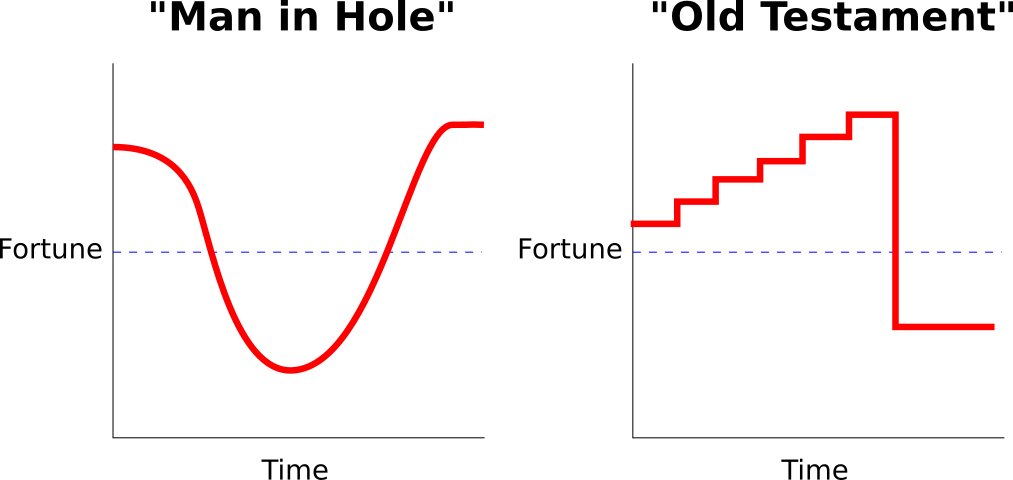
\includegraphics[height=2in]{vonnegut.png}}
\caption{Two of Kurt Vonnegut's ``Shapes of Stories''}\label{fig:vonnegut}
\end{figure}

Although the above lists are useful in the categorisation of different types of
story, they do not tell us about how each story is structured, only the
overarching themes. Author Kurt Vonnegut recognises that a story must also contain
moments of rising and falling action, such as times where the hero experiences a
struggle or climactic victory. In order to describe the ``ups and downs'' of a narrative, Vonnegut describes several different ``shapes'' of stories in his
rejected Master's thesis~\citep{vonnegut2009palm}. He plots the events of a story
as points in a 2D space with ``Beginning-End'' (time) on the X-axis and ``Ill
Fortune-Great Fortune'' (fortune of protagonist) on the Y-axis.
Figure~\ref{fig:vonnegut} shows two examples of story shapes. In the ``Man in
Hole'' example, things start out well for the story's protagonist, but then some
misfortune falls on them. They spend much of the story overcoming challenges
before finally ending the story with a triumph. In the ``Old Testament''
example, the protagonist(s) experience gradually increasing levels of fortune,
before finally being ``cast down'' to a grave level of misfortune at the end of
the story.

All of the above categorisations describe stories as a whole, sorting narratives
into one of several different ``types'' of story. This works well for
linear narratives within traditional media, but what about experimental and
non-linear narratives? In the next section, we review the literature relating to
these less traditional types of stories.

\subsection{Types of Narrative}
\label{sec:narrative-types}
% Author Kurt Vonnegut
% Look at Cybertext, etc, and try to explain how best to divide different types
% of story
The rise of the Web in the 1990s brought with it great interest in the future of narrative in cyberspace. Aarseth's work, \emph{Cybertext} \citep{aarseth1997cybertext} describes the creation of a new form of narrative, for which he coins the term \emph{ergodic literature} (from the Greek words \emph{ergon} and \emph{hodos}, meaning `work' and `path'). In this new form of narrative, some amount of work or effort is required by the reader in order to traverse the path that the story takes.

% scriptons/discourse textons/fabula (Bal 1997)
Aarseth makes a distinction between the narrative as written by the author, and the way in which it is traversed by the reader, calling the former \emph{textons} and the latter \emph{scriptons}. In ergodic literature, the \emph{scripton} is produced by the effort that the reader goes through in interpreting the \emph{texton}. In the context of a game, it is as though the game interface is a gateway that allows access to the narrative at different times. Using classical music as a metaphor, the texton can be thought of as the \emph{score}, and the scripton the \emph{performance}.

% TODO Make sure you update the intro with this
In Section~\ref{sec:interactive-narrative}, we assert that how generative a narrative is and its level of interactivity are two different variables in an experimental narrative. However, Aarseth identifies seven different methods of story traversal: \emph{dynamics, determinability, transiency, perspective, access, linking and user function}.

\textbf{Dynamics} describe whether or not the content and number of scriptons changes. In a simple, static story with branching choices (such as in a \emph{Choose your own adventure} story), both the number of textons and scriptons are fixed, since all paths have been written out beforehand. A dynamic story would still have a fixed number of textons, but the scriptons would be generated as the user traverses the path of the narrative.

\textbf{Determinability} is how deterministic the narrative is, whether or not the same interactions will result in the same scripton being produced.

\textbf{Transiency} means to what extent scriptons are produced as time flows, or whether user interactions are required to produce them.

\textbf{Perspective} is whether or not the user/reader plays a role as a character in the narrative.

\textbf{Access} is whether a user has access to all scriptons at any point in traversing the narrative, or whether their access is restricted.

\textbf{Linking} is whether or not parts of the scripton are linked to other parts, and whether these links are conditional (if they rely on a user having already traversed part of the scripton).
\textbf{User functions:} the functions the user uses to traverse the text. This could be interpretive (which is implicit in any traversal of the text), explorative (traversing the scripton according to whim) or configurative (specifying parts of the scripton in advance), for example.

% Ugh, this is all so arbitrary. Go on to describe Aarseth's PCA of these variables and explain why you don't think it's a good fit.

By performing correspondence analysis (a process similar to principle component analysis) on a diverse corpus of 23 texts ``\emph{ranging from ancient China to the Internet}'', Aarseth filters these seven variables down into two numerical axes which account for 49 percent of the variation between stories. Using these axes, he groups classic tales such as \emph{Moby Dick} and more experimental narratives such as William Gibson's \emph{Agrippa} and Michael Joyce's \emph{Afternoon}. By grouping these stories into categories, he intends to show how emerging media are enabling new types of story.

Chris Crawford's \emph{Chris Crawford on Interactive Storytelling} \citep{crawford2012chris} provides a scathing assessment of the relationship between narrative theory and computer science. A veteran of the games industry, he argues that `soft' science theories such as those of Aarseth et al are entirely removed from `hard' science, and are therefore an example of bubble intellectualism and impossible to implement. 

Crawford himself provides a useful examination of experimental narrative in computer games, defining interactivity as:

\begin{quote}
A cyclic process between two or more active agents in which each agent alternately listens, thinks, and speaks.
\end{quote}

He argues that for game narratives to be truly interactive, they must be more social. Characters in a story must be able to react with the player as though they were people in real life. In turn, the player should have some degree of freedom in the way in which they interact. Rather than presenting branching story points as choices, a better way to interact would be socially, through talking to agents in the game. This is the approach that Fa\c{c}ade takes \citep{mateas2003faccade}, which Crawford acknowledges as the most successful attempt at interactive storytelling to date. A detailed description of Fa\c{c}ade's implementation appears in Section~\ref{sec:drama-systems}.

In order to determine whether Crawford's assertion that narratology research is
too far removed from its practical implementations to be of use, we provide an
overview of these implementations and their underlying research in Section~\ref{sec:implementations}. Has narrative theory research informed the creation of computer-generated or interactive narrative at all, or do they all take approaches grounded in computer science and artificial intelligence? If narrative theory has not been used, then we must ask: why not?


\subsection{Formalisms of Narrative}\changed{}{Renamed section from
  ``Structuralist Formalisms of Narrative'' to just ``Formalisms of Narrative''}
\label{sec:formalisms}

Attempts to organise recurring themes, roles and motifs of narrative go back at least a century. The Aarne-Thompson tale-type index \citep{aarne1987types}, first published in 1910 and later refined by Stith Thompson in 1928 and 1961, is well known amongst folklorists as a classification and analysis method for traditional folktales and myths. Aarne-Thompson's index is a taxonomy of tale themes, arranging tales into categories such as \emph{animal tales} and \emph{jokes and anecdotes}, and then sub-categories (\emph{tales of magic} and \emph{numskull [sic] stories} being two examples). This taxonomy is only two levels deep however, and only serves as a useful way to categorise individual stories or tales. In order to break down and analyse components of tales, we must dig deeper.

In \emph{Structural Anthropology}, Claude L\'{e}vi-Strauss seeks to discover why myths and legends are so similar across cultures and history \citep{levi1963structural}. He concludes that there are global laws that govern the way in which people create stories, therefore these laws can be modelled as a set of rules for describing myths.

His theory is that myths describe opposing forces which are resolved through mediation. The example he gives in \emph{Structural Anthropology} describes how Native American legends often contain `trickster' characters in the form of ravens or coyotes. As scavenging animals, these tricksters symbolically act as mediators between life and death.

Like much of early narrative theory, there is no rigorous evaluation of L\'{e}vi-Strauss' ideas, leaving them seeming opinionated and arbitrary. While interesting, L\'{e}vi-Strauss' ideas bring us no closer to developing a formal model of narrative structure. For that, we must go even further back in time, and turn to Vladimir Propp.

\subsubsection{Propp's Morphology of the Folktale}
\changed{A notable narrative formalist is Vladimir Propp, creator of \emph{The
    Morphology of the Folktale}~\citep{propp1968morphology}, a formalism for
  Russian folktales. Propp's formalism, though originally limited in scope,
  generalises well, and is still used by researchers to procedurally generate
  stories~\citep{grasbon2001morphological,gervas2005story,hartmann2005motif}.}{Propp
is a formalist instead of structuralist} Drawing from a corpus of one hundred Russian folktales, Propp identifies thirty-one distinct \emph{story functions}, each of which is identified by a number and symbol. These functions are executed by characters fulfilling certain roles, each of which has a \emph{sphere of action} consisting of the functions that they are able to perform at any given point of the story. Stories are created by chaining story functions together, with subplots expressed as parallel chains of story functions.

In this formalism, characters have \emph{roles}, such as \emph{hero}, \emph{villain}, \emph{dispatcher}, \emph{false hero}, and more. Characters performing a certain role are able to perform a subset of \emph{story functions}, which are actions that make the narrative progress. For example, the \emph{dispatcher} might send the \emph{hero} on a quest, or the \emph{victim} may issue an \emph{interdiction} to the \emph{villain}, which is then \emph{violated}.

Propp defines a total of 31 distinct story functions, each of which is given a number and symbol in order to create a succinct way of describing entire stories. Examples of such functions are:

\begin{itemize}
  \item One of the members of a family absents himself from home: \emph{absentation}.
  \item An interdiction is addressed to the hero: \emph{interdiction}.
  \item The victim submits to deception and thereby unwittingly helps his enemy: \emph{complicity}.
  \item The villain causes harm or injury to a member of the family: \emph{villainy}.
\end{itemize}

Each of these functions can vary to some degree. For example, the \emph{villainy} function can be realised as one of 19 distinct forms of villainous deed, including \emph{the villain abducts a person}, \emph{the villain seizes the daylight}, and \emph{the villain makes a threat of cannibalism}.

\begin{figure}[!t]
\centerline{
\includegraphics[height=0.4in]{propp1.png}}
\caption{One Propp function following another}\label{fig:propp1}
\end{figure}

\begin{figure}[!t]
\centerline{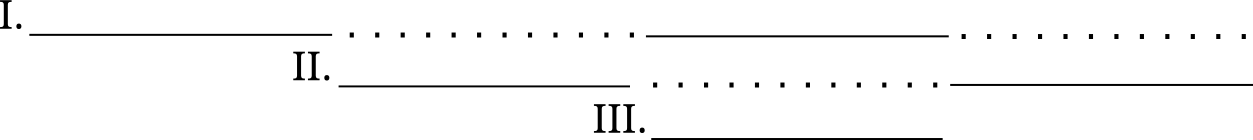
\includegraphics[height=0.6in]{propp2.png}}
\caption{Multiple simultaneous functions}\label{fig:propp2}
\end{figure}

In a typical story, one story function will follow another as the tale progresses in a sequential series of cause and effect (figure~\ref{fig:propp1}). However, Propp's formalism also allows for simultaneous story functions to be occuring at once (figure~\ref{fig:propp2}).

% Though flexible, Propp's formalism is limited in its expressiveness. All story
% functions describe events at the same level of abstraction, describing one event
% after another. Also, Propp insists that the story functions occur in a
% prescribed order. Later French structuralists such as \citet{bremond1980logic},
% \citet{greimas1983structural} and~\citet{todorov1969grammaire} address the
% latter problem by generalising Propp's work outside of Russian Folktales, though
% each represents only incremental improvements on Propp, lacking a means of
% nesting story functions to create abstractions. \citet{barthes1975introduction}
% broadly describe hierarchically composing \emph{narrative units} but, lacking
% implementation details, these can only be used as a template from which to build
% a new narrative model.
\deleted{Removed paragraph about French structuralists}


% What are the shortcomings of Propp? (i.e. lack of abstractability, etc)

% \subsection{Describing Stories with Logic}
% Laure-Ryan did a bit of this, also include linear logic approaches

\subsection{Other Types of ``Story Component''}
Lehnert's \emph{plot units} are a more recent narrative formalism
\citep{lehnert1981plot}. However, these plot units only describe stories as three
types of event: positive, negative and mental. These events occur with respect
to a single character in the story, so an author must always author story
components with concrete characters in mind, making them difficult to re-use.
Similar to Propp's system, the order of composition must always be in a certain
sequence, and plot units cannot refer to other plot units. Again, we are left
without a means of creating abstractions for our story components.
\changed{Chapter~\ref{cha:tropical} addresses this issue by describing how
  tropes allow the nesting of components to allow story authors to create their
  own abstractions.}{Referenced chapter by number instead of name}

\section{Implementations of Experimental Narrative}
\label{sec:implementations}
% I've plenty of material, but it really needs reworking and extending

\subsection{Story Generation}
\label{sec:story-gen}
% TaleSpin, etc
Inspired by Chomsky's theories of generative grammar \citep{chomsky1968sound}, researchers in generative narrative strive to build their own `universal grammar' for narrative.

\begin{figure}[!t]
  \begin{center}
  \begin{enumerate}
    \item $\texttt{Attempt}\rightarrow \texttt{Plan} + \texttt{Application}$\\
           $\qquad\Rightarrow\texttt{MOTIVATE(Plan, Application)}$
    \item $\texttt{Application}\rightarrow\texttt{(Preaction)*} + \texttt{Action} + \texttt{Consequence}$\\
           $\qquad\Rightarrow\texttt{Allow(AND(Preaction,Preaction,...),}$\\
           $\qquad\{\texttt{CAUSE | INITIATE | ALLOW}\}\texttt{(Action,Consequence)}$
  \end{enumerate}
  \end{center}

  \caption{Example rules from Rumelhart's story grammar}\label{fig:rumelhart}
\end{figure}

\citet{rumelhart1975notes} provides one early and influential model for the
grammatical generation of natural language. Figure~\ref{fig:rumelhart} shows two
example rewrite rules from this grammar. Each rule pair consists of a
syntactic rule (following the `$\rightarrow$' symbol) and a semantic
interpretation rule (following the `$\Rightarrow$' symbol). The `+' symbol denotes items happening in a sequence, the `\textbar' showing possible alternatives. `*' denotes one or more item being generated. Capitalised words (such as ALLOW, MOTIVATE, etc) describe relationships between items. For example, MOTIVATE is a relationship between a character's thought and their reaction to that thought.

Other systems draw inspiration from generative grammar, such as GESTER \citep{pemberton1989modular}, which generates stories based on a grammar synthesised from old French epic tales. \citet{lang1999declarative} describes a declarative model for narrative, consisting of lists of first-order predicate calculus expressions. These expressions describe events, states, goals and beliefs which combine to form a narrative. More specifically, it combines:

\begin{itemize}
  \item A \textbf{grammar interpreter} to search for a sequence of grammar rewrites which would produce a convincing narrative.
  \item A set of \textbf{temporal predicates} to describe the occurence of events over time and enforce temporal constraints on story components.
  \item A \textbf{world model} which describes the set of actions that characters may perform and fluents that may alter over the course of the narrative.
  \item A \textbf{natural language output unit}, which takes the sequence of events produced by the story grammar and converts it into readable natural language sentences.
\end{itemize}

This combination of using a grammar interpreter, world model and natural language output unit is especially common amongst generative grammar approaches.

While generative grammar approaches may be effective for procedurally creating
prose, they are less well suited to the creation of \emph{interactive}
narratives. Once the grammar rewrite rules are specified, the user is entirely
passive, unable to affect the way in which the story is being generated. For
this to happen, the narrative needs to be part of a system that reacts to the
actions of the user, such as in a computer game.

\begin{figure}[!t]
\begin{quote}
  ONCE UPON A TIME GEORGE ANT LIVED NEAR A PATCH OF GROUND. THERE WAS A NEST IN AN ASH TREE. WILMA BIRD LIVED IN THE NEST. THERE WAS SOME WATER IN A RIVER. WILMA KNEW THAT THE WATER WAS IN THE RIVER. GEORGE KNEW THAT THE WATER WAS IN THE RIVER. ONE DAY WILMA WAS VERY THIRSTY. WILMA WANTED TO GET NEAR SOME WATER. WILMA FLEW FROM HER NEST ACROSS THE MEADOW THROUGH A VALLEY TO THE RIVER. WILMA DRANK THE WATER. WILMA WASN'T THIRSTY ANYMORE.

GEORGE WAS VERY THIRSTY. GEORGE WANTED TO GET NEAR SOME WATER. GEORGE WALKED FROM HIS PATCH OF GROUND ACROSS THE MEADOW THROUGH THE VALLEY TO A RIVER. GEORGE FELL INTO THE WATER. GEORGE WANTED TO GET NEAR THE VALLEY. GEORGE COULDN'T GET NEAR THE VALLEY. GEORGE WANTED TO GET NEAR THE MEADOW. GEORGE COULDN'T GET NEAR THE MEADOW. WILMA WANTED TO GET NEAR GEORGE. WILMA GRABBED GEORGE WITH HER CLAW. WILMA TOOK GEORGE FROM THE RIVER THROUGH THE VALLEY TO THE MEADOW. GEORGE WAS DEVOTED TO WILMA. GEORGE OWED EVERYTHING TO WILMA. WILMA LET GO OF GEORGE. GEORGE FELL TO THE MEADOW. THE END.
\end{quote}
\caption{Example TALE-SPIN output}\label{fig:tspin}
\end{figure}

% TODO elaborate on this
James Meehan's TALE-SPIN \citep{meehan1977tale} is an influential early approach to story generation using planning. In TALE-SPIN, the author describes a story domain, its characters and their goals, and a natural language story is produced as output. It works by using a problem-solver to resolve each character's goals over the story domain. Figure~\ref{fig:tspin} is an example of TALE-SPIN's output.

TALE-SPIN's strong planning component is evident in the reading of its output. Sentences are terse, with one event leading directly to another in order to achieve some goal. One problem with this character-led approach is that the goals of the author are not necessarily taken into account. If the author intends for a character to die at some point in the story, it seems unnatural for a character to have the goal of dying to fulfill this intention.

 Turner criticises TALE-SPIN's stories as seeming ``pointless and somewhat boring'' \citep{turner1986thematic}, going on to create the MINSTREL system for story generation \citep{turner1993minstrel}. Using the legendary world of King Arthur's court as a story domain, MINSTREL strives to generate stories with an authorial purpose.

MINSTREL attempts to address TALE-SPIN's shortcomings by introducing two types of schema: author-schemas and character-schemas, both of which combine to represent the elements of a story. The author-schemas describe the goals of the author of the system, allowing story creators more control over the structure and content of their narrative. This allows authors to specify a `point' or moral to their story, something that is not possible to achieve with TALE-SPIN. Character-schemas describe character-level goals in a similar manner to those of TALE-SPIN's.

The comparison of TALE-SPIN and MINSTREL highlights a challenge that has
dominated story generation for decades: the balance of \emph{character} and
\emph{plot} (as~\citet{riedl2010narrative} highlights). Especially with approaches based on multi-agent systems, the regulation of character actions to conform to an underlying theme or structure is a challenging problem.

However, modelling characters with agents is a promising approach to take in order to achieve a story which is both generative and interactive. In such a system, an author can specify the story world and character models, creating the `big picture', and the agents would be able to fill in the details (such as dialogue, sub-plots, and relationships).
An apt metaphor would be that of animation. In large animation studios such as
Disney, the lead animator draws the key frames of a sequence, and a team of
other animators work to fill in the gaps in
between\footnote{This process is described at the following website:
  \url{http://www.justdisney.com/animation/animation.html}, accessed 20160805.}. This is what the combination of a managed narrative with agents could achieve: the author would be the `lead animator' in such a system, with the agents being the assistants.

The implementations until now have focused mainly on \emph{generation\/}, and little on \emph{interaction\/}. Character models have been mentioned, but these do not react in real time to a user. For that, we need a multi-agent system.

\subsection{Characters as Intelligent Agents}
Story worlds are usually populated with characters. Interactive story worlds
such as games contain characters with very basic scripted behaviour. At even the
highest level of game character simulation, AI techniques are usually used to
govern basic behaviour such as movements and actions. Governing character
behaviour to fit within the context of a narrative is a more challenging
problem. This section examines different approaches to tackling this challenge.

\subsubsection{Planner-based Systems}
\label{sec:planner-systems}
The most prevalent approach to the generation and management of plot in
interactive narrative is to use planners. With a planner, an author sets the
goals for the story (certain situations that they would like to see happen), and
the planner tells the character agents what to do to make sure these ``story
goals'' are achieved. When a player that is interacting with the system takes an
action that compromises the story goals, the planner must re-plan to make sure
the goals can still be achieved, by restricting the actions of the player or
intervening in some other manner.

% This needs elaboration
\citet{young1999notes} argues that planners are a good method for regulating
plot, later creating the \emph{Mimesis} architecture for integrating a planner with character agents in an interactive game environment, \citep{young2004architecture}. Young describes how narrative systems must re-plan when a player makes  narrative-breaking actions, by either restructuring the narrative mid-story (\emph{accommodating} the action) or preventing the action from executing (\emph{intervening} on the action).

Given its influence over subsequent approaches to interactive narrative
generation, it is worth looking at the Mimesis architecture more closely.
It is designed to integrate into the \emph{Unreal
  Tournament} game engine, and has five components: the \emph{mimesis
  controller}, the \emph{story planner}, the \emph{discourse planner}, the
\emph{execution manager} and the \emph{MWorld}.

Figure~\ref{fig:mimesis} shows how these components work together to form the
Mimesis architecture. Once an author has created the pre-defined libraries of
actions needed by the story planner, the following steps are taken to determine
the course of the story:

\begin{enumerate}
  \item All the components connect to the Mimesis Controller (MC) via socket
    connection. It then acts as a message router.
  \item The game initiates a plan request containing the state of the game
    world, a list of possible actions, and the goals for the plan.
  \item The \emph{story planner} responds with a \emph{story world plan}, a data
    structure that describes the actions (selected from the list) that must occur over time in order to
    meet the plan request's goals.
  \item Once the story world plan is created, it is sent to the \emph{discourse
      planner}, along with a list of actions that can occur in the game engine
    (such as camera movements, voice-overs and background
    music). The discourse planner then creates a sequence of these actions that
    best fit the story world plan.
  \item The discourse planner then sends the narrative plan to the
    \emph{execution manager}, which builds a directed acyclic graph (DAG), where
    the nodes are the actions within the plan and the edges are the temporal
    constraints between the orderings of the actions. The execution manager
    removes nodes from the DAG in order, sends the node's actions to the
    game engine, and updates the graph.
  \item The \emph{MWorld} is essentially the environment in which the story
    occurs, consisting of the game engine, coordination code, and class
    definitions for actions, and discourse planners. It is the MWorld that
    receives actions from the execution manager to be executed, and executes
    these actions in the game engine.
\end{enumerate}

Mimesis uses DPOCL (Decomposed Partial-Order Causal-Link Planner,~\citep{young1994decomposition}) plans for
its story planning. DPOCL plans are composed of \emph{steps} (the plan's
actions), \emph{ordering constraints}, \emph{decomposition links} describing the
hierarchical structure of a plan, and \emph{causal links} between pairs of
steps. It uses \emph{refinement search} \citep{kambhampati1995planning} as its
plan reasoning process, searching through the space of possible plans represented as a directed
graph, with each node in the graph being a plan or partial plan. Mimesis
specifies the initial planning problem for DPOCL using the current and goal
states of the story.

A key feature of Mimesis is its strategies for handling of user actions which potentially
interfere with the story plan, making its goals unachievable. In the intervention strategy, Mimesis simply prevents the
user's action from having any effect in the game world. With accommodation,
Mimesis replans the story events, restructuring the plan so that the interfering
actions are taken into account and worked around.

\begin{figure}[!t]
\centerline{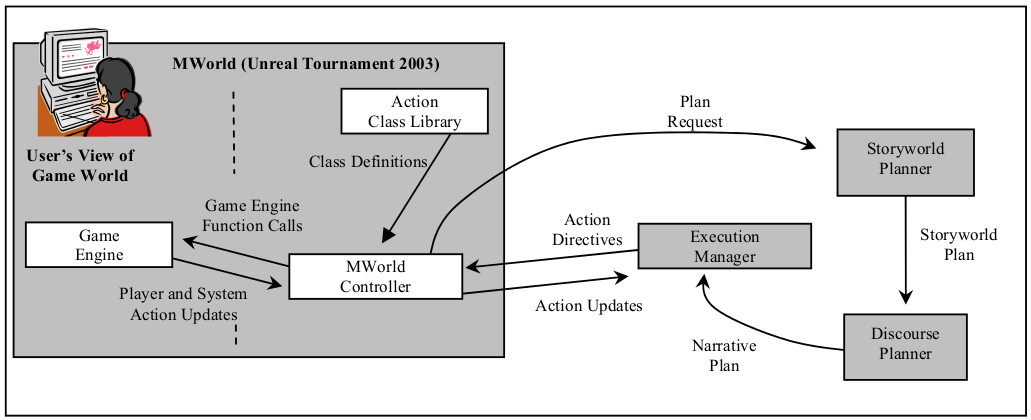
\includegraphics[height=2in]{mimesis.png}}
\caption{The Mimesis architecture, from \citet{young2004architecture}}\label{fig:mimesis}
\end{figure}

% This needs elaboration
\citet{cavazza2002character}'s \emph{I-Storytelling} system implements
\citet{young2004architecture}'s architecture with ideas from Barthes' narrative
units~\citep{barthes1975introduction}, using characters with behaviour described
by Hierarchical Task Networks (HTNs) to generate its stories. Each character has a main task, which is divided into subtasks to create a task hierarchy, with each task node having pre- and post-conditions. The story emerges from the outcomes of each character's plans, and the narrative structure as a whole is not planned.

% This needs elaboration
\citet{riedl2003managing} describes a further development of Young's architecture,
allowing the story author to create plans for the overall narrative in addition
to its characters.
Rather than using a narrative model, this version of Mimesis models the player to track their expected level of suspense while interacting with the story. Like the \emph{I-storytelling} system, its plans are hierarchical, using the Longbow hierarchical partial-order causal link planning system~\citep{young1994decomposition}.

A disadvantage of these planner-based systems is that they require the story
author to think in a planner-oriented manner. They must consider the goals of
both the story and the character, plans to achieve these goals, and re-planning
when goals are not met or when situations change. This is a drastic change from
the usual story writing methods of authors, where the focus is on structure,
plot, themes and characters. Though graphical user interfaces such as Mimesis'
Bowman system~\citep{thomas2006author} could be used to assist plan-driven
story authoring, a complete shift in creative workflow is still required, making
this approach inaccessible to non-technical writers.

% This needs elaboration
\subsubsection{Drama manager-based Systems}
\label{sec:drama-systems}

Carnegie Mellon University's OZ project \citep{mateas1999oz} uses a \emph{drama
  manager} to structure its narrative, which observes the actions occurring in
the storyworld and ``directs'' its characters to conform to shape the story. A
screenshot from the game is shown in Figure~\ref{fig:facade-screen}.

\begin{figure}[!t]
\centerline{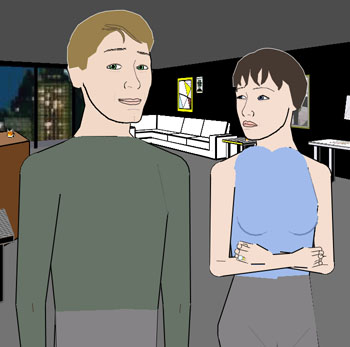
\includegraphics[height=2.5in]{facade.jpg}}
\caption{A screenshot from \emph{Fa\c{c}ade} \citep{mateas2003faccade}}\label{fig:facade-screen}
\end{figure}

Mateas and Stern's \emph{Fa\c{c}ade}~\citep{mateas2003faccade} has players interact with the characters of the story through natural language. In this game, the player attends the party of a young couple (Grace and Trip) celebrating their wedding anniversary. As the course of events unfold however, the player learns that all is not as happy as it seems.

The player interacts with the characters by typing in natural language
sentences, to which Grace and Trip respond. Though the characters are
implemented through agents, the story is controlled using a drama manager. In
all, their system consists of using Natural Language Processing (NLP), a novel character authoring language and a novel drama manager to create an interactive narrative.

Several custom-designed languages were used to create the game, including a language called `A Behaviour Language' (ABL) for the agents and a special language for the sequencing of the beats. ABL represents situations as character goals, maintaining a tree of all the active goals and behaviours that are happening at any time.

In Fa\c{c}ade, the smallest unit of narrative action is called a \emph{story beat}, taken from McKee's book on authorial style for screenwriters \citep{mckee1997substance}. The simulation constantly monitors what the user is doing and how it may lead from the current story beat to another. Story beats have preconditions and effects on the state of the narrative, so it is the drama manager's job to work out when it makes sense to initiate a certain beat.

`Beats' have a very fine granularity, with 200 or so updating every minute of the simulation. They consist of a set of ABL behaviours, which advance the narrative yet still allow interaction to change to other beats. Only one beat can be active at a time.

A beat can have 5 types of goal:

\begin{itemize}
  \item \textbf{Transition-in:} characters express their intentions
  \item \textbf{Body:} a dramatic question/situation is posed to the player
  \item \textbf{Local/global mix-in:} react to the player before end of the beat
  \item \textbf{Wait-with-timeout:} wait for the player's reaction
  \item \textbf{Transition-out:} final reaction to the player's action in the beat
\end{itemize}

A beat goal is a series of steps for an agent to perform, which can be:

\begin{itemize}
  \item staging (where to walk to, face)
  \item dialogue to speak
  \item where and how to gaze
  \item arm gestures to perform
  \item facial expression to perform
  \item head and face gestures to perform
  \item small arm and head emphasis motions triggered by dialogue (head nods, hand flourishes)
\end{itemize}

As an example, there is a behaviour called ``Fix\_Drinks'', which specifies a sequence of agent behaviours where the characters Grace and Trip have an argument while Trip asks the player what they would like to drink. If the player decides not to go along with the beat (in this case, by not choosing a drink), then the beat will be aborted and replaced with another.

Fa\c{c}ade has become popular as a game outside of academia, with playthroughs of the game reaching millions of views on Youtube. This shows the promise of interactive narrative as being a unique and engaging new form of entertainment. Unfortunately, no other implementation of interactive narrative seems to have captured the public imagination since the release of Fa\c{c}ade.

Fa\c{c}ade's popularity seems to reinforce Crawford's assertion (as we mention
in Section~\ref{sec:narrative-types}) that interactive narratives must be social
in nature. The gameplay comes entirely from the conversations and interactions
between Grace, Trip and the player. Much of the excitement comes from the social
consequences of certain conversation paths or actions. \changed{By modelling characters
as agents, Mateas and Stern~\cite{mateas2003faccade} have created a truly
interactive experience. However, by also using a drama manager to manage the
agents, they have used these agents to tell a story.}{Replaced Mateas et al with
bibtex reference}

How might these agents be made more convincing? Outside of writing rules for their behaviour consisting of character goals and beliefs, how might an author create truly unique and idiosyncratic characters? To address the question, we next examine different types of emotional models in psychology, and how each might be used to model characters as agents.

\subsubsection{Social Norms}
Versu~\citep{evans2014versu} is an interactive drama system that uses a multi agent system as characters. The characters' actions are coordinated with \emph{social practices}, which describe types of social situations and is described by the authors as a successor to the Schankian script. These social practices are implemented as reactive joint plans, which agents can choose to participate in or not. Rather than directly telling the agents what to do, these social practices merely \emph{suggest} courses of action, leaving each agent to decide for itself what to do based on its individual goals.

The authors decide against using a drama manager to control the agents' actions because they want to take the \emph{strong autonomy} approach to agent governance. This means that they prefer to give each agent some degree of autonomy by allowing it to make the final decision on which course of action to take, rather than blindly following a drama manager. Suggesting actions with social norms achieves this goal. Rather than describing typical story events in terms of social norms, however, in Versu the social norms \emph{are} the story. The gameplay revolves around the avoidance (or purposeful subvertion of) awkward social situations.

Each character has a role, which is governed by a social practice. For example, a \emph{greeting} practice involves characters with the \emph{greeter} and recipient roles. The greeting practice would tell the greeter in which manner they are to greet the recipient, and the recipient how to respond. It is noteworthy that these actions are merely suggested, and not enforced.

\emph{Exclusion logic}~\citep{evans2010introducing} is used to describe the
social practices of the system. Exclusion logic manages the frame problem by
organising related fluents in a tree structure. A single update at the right
branch can change a set of related facts en masse. This is achieved through use
of an exclusion operator (``!''). Listing~\ref{lst:exclusion1} shows an example
of the exclusion operator in use. The example specifies that an agent can have
only one gender. The \emph{Praxis} language implementation of the exclusion
logic in Listing~\ref{lst:exclusion1} has a type checker which ensures that no character can have multiple genders.

\begin{lstlisting}[float,label=lst:exclusion1,caption=nextHopInfo: caption]
A(agent).sex!G(gender).
\end{lstlisting}

\begin{lstlisting}[float,label=lst:exclusion2,caption=Description of ``Brown'' character.]
brown.sex!male;
brown.class!upper;
brown.in!living_room;
brown.in.living_room.activity!watching_tv;
brown.relationship.lucy.evaluation.attractive!40;
brown.relationship.lucy.evaluation.humour!20.
\end{lstlisting}

Listing~\ref{lst:exclusion2} is another piece of \emph{Praxis} code showing how the attributes of a character called
``Brown'' are built up as a tree structure.
Exclusion logic's exclusion operator allows an author to express the fact that a
variable can only have one value. For example, if `the `Brown'' character
changes location from the living room to the kitchen,
\emph{brown.in!living\_room} is terminated when \emph{brown.in!kitchen} holds.
This also terminates any attributes further down the tree, so in this case the
\emph{brown.in.living\_room.activity} of \emph{watching_tv} will also be
terminated when the location updates.

Versu takes the \emph{constitutive} view of social practice, as opposed to the
\emph{regulative} view~\citep{SJP:SJP658}. This means that rather than restricting an agent's possible actions based on its permissions and obligations, they participate in a certain social practice by taking an action. Their actions are only restricted by what is possible in the story world, and what the agent desires to do. This way, agents can choose whether or not to take part in certain social interactions.

Many of the components we aim to have in our story telling system appear in Versu: the use of social norms to gently encourage story-conforming behaviour rather than demanding it, and the use of formal logic to determine which behaviours are possible. However in Versu the social norms \emph{are} the story, rather than describing the story components that invisibly govern the behaviour of characters. In order for this kind of governance to occur, an institution-based solution is preferable, based on events, agent actions and standard deontic logic. Because character actions are constrained by the structure of a story, a \emph{regulative}  view of social practice is more suited to the expression of story components as social norms.

Many of the advantages of using exclusion logic can be gained by using an institution-based approach. Non-inertial fluents can be used to ensure that variables can only ever have one value. Standard deontic logic~\citep{von1951deontic} is enough to provide the rest of what is needed.

% Need at least one more example here
\subsection{Modelling Narrative with Logic}
\label{sec:model-logic}
Although most recent research focuses on the use of planners to manage the drama in a story, there is also much interesting work which makes use of formal logic to model narrative. Though often used for the generation of linear story text, it is increasingly being applied to non-linear narratives as well. Logic-based approaches are generally based on either temporal logic variants or some kind of linear logic.

Ceptre~\citep{martens2015ceptre} is a language for modelling generative interactive narratives using \emph{linear logic}, a formal logic designed to describe resource usage. 

A Ceptre story begins with an initial state $\Delta_0$. Each state iteration
$\Delta_i$ is examined repeatedly, and a subset $S$ of it is updated with rule
$r$. The next state, $\Delta_{i+1}$, has the subset $S$ replaced with $S'$, the
new subset with the consequences of the applied rule $r$.

The rules are specified using the combination of logical statements with two
operators: $*$ (tensor) and $\text{-o}$ (lolli). The tensor operator is used to
concatenate statements, while the lolli operator expresses state transitions in
the form $S \mathrel{\text{-o}} S''$. The rules use \emph{replacement semantics},
which means that everything from state $S$ will disappear unless stated to be in
state $S'$. A $\$$ operator is used to mark facts in $S$ that the author wishes
to remain in $S$ without explicitly stating so.

Listing~\ref{lst:ceptre-murder} shows an example from~\citet{martens2015ceptre}
that describes a ``murder'' rule and its consequences.

\begin{lstlisting}[label=lst:ceptre-murder,showstringspaces=false]
do/murder
    : anger C C' * anger C C' * anger C C' * anger C C' *
    $at C L * at C' L * $has C weapon
    -o !dead C'.
\end{lstlisting}

In this case, four instances of the ``anger'' predicate with the same arguments
has a significant meaning: a character's emotion is treated as a resource. The
fact that \emph{anger $C C'$} appears four times means that a character is
\emph{four times} as angry at another character. Depending on how many times the
``anger'' statements appear in the new state, this anger can rise or fall at the
next step in the story. In this case, the emotion is not only treated as a
pre-condition, but also as a resource. These resources can also be specified
through the addition of a number to the name of the resource.

Ceptre introduces a \emph{stages} feature that allow authors to structure a
program through the use of independent components. A stage is a unit of
computation that runs to quiescence, meaning that it terminates when no more
rules are able to fire. At this point, another stage may commence.

The central motivation behind Ceptre's design is its ability to use ``proofs as
traces'', or \emph{computation as proof search}~\citep{hodas1991logic}. Ceptre
uses a \emph{sequent calculus}, where a sequent $\Delta \vdash A$, $\Delta$ is a
state, and $A$ is a goal formula. If a complete proof tree can be formed with
that sequent as its root, then the sequent can be said to be \emph{derivable}.
Thus Ceptre takes a sequent as input and creates a proof as output, declaring
failure if a proof cannot be created. Ceptre looks at the left side of the
sequent, using \emph{forward chaining} to choose which rules to try in order to
reach the goal formula.

A key feature of Ceptre is its representation of resource management in stories.
Rules are able to either produce or consume resources. This has interesting
implications for the representation of causal structure in linear logic. For
example, if two rule applications consume different sets of resources from the
same state, they are occurring concurrently and independently. However, if one
rule produces resources that are consumed by another rule, then these rules have
a causal, dependent relationship.

This modelling of gameplay as proof search is similar to the technique we use in
Section~\ref{sec:kripke}, where we use Interval Temporal Logic and Kripke structures to
theorem-prove certain narrative states. The difference is that the system we
describe is more concerned with representing different temporal relations,
whereas Ceptre's focus is on resource management within a game.

\subsection{Normative Frameworks for Multi-Agent Systems}\label{sec:lit-insts}
\emph{Social Institutions} (or \emph{Normative Frameworks}) govern the behaviour
of agents within a multi-agent system. The agents act according to norms
described within the institutions that govern their society, which act as a
social contract that the agents follow in order to cooperate. We use these
institutions to govern the character agents in our story world (described in
Chapter~\ref{cha:institutions}) because they regulate agent behaviour without
strict enforcement of their actions. This gives the characters in a story the
autonomy to break away from a predefined narrative in certain situations.

Noriega's Ph.D. thesis~\citep{noriega1999agent} uses a fish market as a metaphor for
institutional governance of agents. The thesis explains that Spanish fish
markets seem to use a \emph{downward-bidding} auction protocol that emerges from
a social institution with refined, socially acknowledged conventions. Noriega
explains how agent-mediated institutions may use these social conventions to
model such a market, with an agent governor to ensure that the conventions are enforced.

The idea of agent ``societies'' being governed by social conventions is realised
through several different implementations. \citet{artikis2009specifying} present
a framework for the executable specification of open agent societies, where an
open society is one with heterogeneous agents, conflicting individual goals and
unpredictable behaviour. Emphasis is put on the fact that individuals in such
societies can choose to ignore the social norms that govern them, so long as
they are willing to accept the consequences of non-compliance. Their system is
specified using two action languages (languages for specifying state transition
systems): the $\mathcal{C}+$ language~\citep{giunchiglia2001causal, giunchiglia2004nonmonotonic} and the Event
Calculus~\citep{kowalski1986logic, shanahan1999event}. The models are
executing using the Causal Calculator, a software implementation of
$\mathcal{C}+$. The social constraints of their agent society are expressed in
terms of:

\begin{itemize}
  \item The agents' physical capabilities
  \item Institutionalised powers
  \item Permissions, prohibitions and obligations of the agents
  \item Sanctions and enforcement policies that deal with the consequence of
    non-compliance with obligations and performance of forbidden actions
\end{itemize}

Each agent in the society is assigned a social role that determines its
permitted and obliged behaviours. The social constraints defined in $\mathcal{C}+$
are described in terms of \emph{fluents} (symbols that characterise a state) and
\emph{actions} (symbols that characterise state transitions).

\citet{fornara2007agent} propose a model for the definition
of ``artificial institutions'' for the governance of open multi-agent system societies. They use the notion of \emph{social
  commitment} to define the semantics of an Agent Communication Language (ACL).
Commitments, being objective and external to an agent's internal state,
make it possible to verify whether or not an agent is conforming to the rules of its
society. The authors use \emph{norms} as event-driven rules that create or
cancel sets of social commitments, and are triggered by events that occur in the
multi-agent system. These norms are expressed as \emph{obligations} and
\emph{prohibitions} on the agents'' actions. The system proposed consists of:

\begin{itemize}
\item A set of \emph{entities} that have \emph{natural} or \emph{institutional}
  attributes, where natural attributes reflect physical properties of the
  agents' world (such as the colour of a book), and institutional attributes
  reflect properties that only exist due to agreement between the agents (such
  as the price of a book).
\item \emph{Instrumental actions}, which are actions that occur in the agents'
  physical environment, possibly triggering institutional actions.
\item \emph{Institutional actions}, which are events that change institutional
  attributes, with preconditions and postconditions.
\item \emph{Conventions}, which are the norms triggered by the institutional
  actions in the system.
\end{itemize}

\citet{cardoso2007institutional} describe the creation of ``virtual
organisations'', where agent cooperation is regulated by appropriate norms. In
this case, the enforcement of the institutional norms (``Institutional
Reality'') is carried out by agents
performing roles with certain institutional powers. The implementation of their
system (the ``Institutional Reality Engine'') uses a rule-based inference engine
to determine when norms are violated or fulfilled.

\citet{cliffe2007specifying} develop \emph{InstAL}, the Institution Action
Language, a domain-specific language for the specification of social
institutions that govern the behaviour of multi-agent systems. An InstAL
institution consists of:

\begin{itemize}
\item \emph{Domain fluents}: symbols to track the state of the institution.
\item \emph{Institutional Empowerments}: rules that determine which events have
  the institutional power to occur.
\item \emph{Exogeneous (or external) Events}: these resemble the instrumental actions
  of~\citet{fornara2007agent}'s system, as they describe the actions that occur
  in the agents' physical environment.
\item \emph{Institutional Events}: these events are the same
  as~\citet{fornara2007agent}'s institutional actions, which are events that are
  triggered by exogeneous events and occur within the institution.
\item \emph{Violation Events}: these are events that are triggered when a
  forbidden action is carried out, or if an obligation is not met, acting as the
  punishment for non-compliance.
\item \emph{Permissions}: the set of actions that agents are allowed to carry out.
\item \emph{Obligations}: the set of actions that agents are expected to take
  before certain deadlines.
\end{itemize}

Section~\ref{sec:pjexample} contains a more detailed description of the InstAL
semantics, including an example of how a scene from the ``Punch and Judy''
story is expressed as an InstAL institution. This example is then expressed in
InstAL syntax in Section~\ref{sec:arch-mas}.

\subsection{Modelling Characters with Emotional Models}\label{sec:emotional-models}
In this section, we examine the use of emotional models in intelligent agents,
so that we may create more ``believable'' characters to add to our stories. Part
of the motivation for governing our character agents with the kind of social
institution described in Section~\ref{sec:lit-insts} is so that the characters
are able to break away from the path of the story in ``extreme'' circumstances.
When agents are created with an emotional model, their emotions would be one way
to provide such circumstances, allowing them to deviate from the narrative at
times of extreme emotional distress. The reasoning behind this is described further in the introduction to
Chapter~\ref{cha:institutions}.

Usually it would seem odd to want to model emotion as part of a computational process. Emotion is such a seemingly irrational set of behaviours that they are easy to dismiss as `human imperfections'. However, as \citet{gratch2004domain} observe, emotions may have a useful role to play in communication, so long as they are displayed at appropriate times.

For example, anger prepares the human body to fight by increasing the production of adrenaline. Fear similarly triggers the `fight or flight' response, alerting the senses for danger and preparing the body to react.

In order to model human emotions using agents, we must first find a suitable psychological model to use. Marsella et al describe three main types of emotional model:

\begin{enumerate}
 \item \textbf{Discrete} emotional models, which claim that humans have a set of innate, pre-defined emotional states which people may enter and leave.
 \item \textbf{Dimensional} models of emotion, describing the spectrum of emotions as being points somewhere in continuous space. Implementations typically use two or three dimensions for simplicity.
 \item \textbf{Appraisal} theories of emotion take an agent's mental processes into account. Their emotional state is derived from whether or not their goals have been achieved, and what effects current events are having on their circumstances, for example.
\end{enumerate}

% Give examples of concrete models for each type.
\subsubsection{`Basic' emotions}
Ekman first made a case for discrete, biologically-determined emotions, based on evidence from research into facial expressions \citep{ekman1992argument}. He describes emotions as being \emph{basic}, in two senses of the word: \emph{i.} that there are a number of distinct emotions, each with its own different characteristics, and \emph{ii.} that these emotions were developed through evolution for specific functions.

Ekman argues that these evolved emotions share nine characteristics:

\begin{enumerate}
  \item Distinctive universal signals
  \item Presence in other primates
  \item Distinctive physiology
  \item Distinctive universals in antecedent events
  \item Coherence among emotional response
  \item Quick onset
  \item Brief duration
  \item Automatic appraisal
  \item Unbidden occurrence
\end{enumerate}

These characteristics are shared by all of the `basic' emotions as observed in humans and primates.

Discrete models of emotion suggest that there is a neural basis for emotion. For example, Armony et al describe how the amygdala in the brain is responsible for conditioned fear responses, and created a neural network to model it \citep{armony1997computational}.

Using a discrete model of emotion for agent-based characters would be relatively simple. Each basic emotion could have its own distinct set of behaviours as consequences, and triggering circumstances as preconditions.

However, a more fluid approach could be useful when modelling emotions with agents. It would be impossible to say that an agent is \emph{angry and approaching furious} using a discrete theory of emotion. Nuanced levels of emotion and even combinations of several emotions add an extra level of texture to a character. Dimensional and appraisal theories of emotion address this challenge.

\subsubsection{Russell's circumplex model of emotion}\label{sec:circumplex}
\begin{figure}[!t]
\centerline{
\includegraphics[height=3in]{circumplex.png}}
\caption{Russell's circumplex model of emotion} \label{fig:circumplex}
\end{figure}

Russell's circumplex model of emotion is a well-known dimensional model \citep{russell1980circumplex}. In this case, the dimensional variables are \emph{valence} (how agreeable or otherwise a situation is to an agent) and \emph{arousal} (how excited an agent is).

Russell's original paper proposes a model similar to that shown in Figure~\ref{fig:circumplex}, where the $x$ axis is a person's valence level and the $y$ axis is their arousal level. He argues that the full range of human emotions lie as points along these axes. Eight such examples are shown in Figure~\ref{fig:circumplex}.

This model is very easy to adapt to human-like agents. \citet{ahn2012nvc} adapt
this model by adding a third dimension, dominance, to create conversational
agents in a 3D environment. This `dominance' dimension was first proposed in
Mehrabian and Russell's original work \citep{mehrabian1974approach}, but later
removed due to being perceived as the consequences of the \emph{effects\/} of
emotion \citep{russell1980circumplex}, rather than being a component of emotion
itself. Like Ahn et al, we found it useful to add the dominance-submission
dimension, and so left it in our emotional model. This is the approach we take in creating my Punch and Judy simulation, and so it is described in more detail in Section~\ref{sec:emotion}.

\subsubsection{Appraisal theory}
Appraisal theories of emotion lend well to simulation with agents, due to their taking a person's beliefs, desires and intentions into account with respect to external events. Emotions arise when an event occurs and a person internally \emph{appraises} its consequences with respect to their beliefs, desires and intentions. This fits well with the popular BDI architecture for intelligent agents.

Different methods of appraisal may be used in order to produce emotions. \citet{gratch2004domain} use decision theoretic plans, but other approaches could include reactive plans, Markov-decision processes, or detailed cognitive models.

Though the Punch and Judy simulation described in Section~\ref{sec:punchjudy}
uses a dimensional model of emotion, an appraisal-based model would be worth
investigating due to its tight coupling with belief desire intention
psychological models used in agents.

\subsection{Discussion}\label{sec:litrev-discussion}
\deleted{2.2.2: Removed critique of planner-based systems and the requirements
  that emerged from that discussion}

\changed{Most narrative generation systems make use of formalisms such as
Propp~\citep{propp1968morphology} in order to generate different parts of a
story. Though Propp's system predates computational narrative generation by several decades, neither narrative nor AI research have produced a formalism for
narrative components to replace it entirely. This is likely because Propp's formalism
is ``good enough'', and has worked for most researchers that have used it. There
is also likely to be a network effect, where Propp has become the formalism that
most researchers have heard of, and therefore the one that they end up
using.}{2.2.2: Revised to give Propp the credit he deserves}

Though there have been attempts to create more expressive formalisms as
described in Section~\ref{sec:formalisms}, none have been expressive enough to
overcome Propp's ``good enough'' properties. In order for a story model to
significantly improve upon Propp, it should add features that it and other
existing formalisms lack. We identify these features as:

\begin{itemize}
  \item A means of \emph{abstraction}
  \item Conceptually \emph{simple} enough for non-programmers to grasp
  \item A library of re-usable \emph{examples} for authors and researchers
\end{itemize}

\paragraph{A Means of Abstraction}
Current narrative formalisms lack a means of \emph{abstraction}. Propp,
for example, describes events in stories that all occur at the same level of
abstraction. This means that one is limited to describing events that occur one
after another, or in parallel, but not events that contain sub-events.

For example, suppose we define a ``Quest'' component of a story, which describes a
sequence of events that occur (such as the hero leaving home and then defeating
a monster). It is easy to think of other story components that could contain
this ``Quest'' component, such as ``Hero's Journey'', ``Rescue the World'' or
``Rite of Passage'' story components. These components could themselves be used
as part of other components. This gives us a means of creating abstractable,
reusable story components. Of all the story models described in
Section~\ref{sec:formalisms}, none have any means of abstraction such as this.

The example we just described already hints at the use of story tropes that
contain other tropes. This is the means of abstraction and re-use that we use in
our system, described in Chapter~\ref{cha:tropes}.

\paragraph{Conceptually Simple}
Story authoring tools are user interfaces which are used to write fiction. In
the computing world, user interfaces are often simplified through the use of an
\emph{analogy}. For example, a \emph{Desktop Environment} is a graphical user
interface analogy created by Xerox in the 1970s. Where computer users would
previously have had to learn and master a complicated command-line interface,
the desktop environment metaphor presented an interface that resembled something
that users were already familiar with: the top of a desk, with icons
representing files spread out over a ``desktop'' surface.

When creating a story model, it is easy to fall into the trap of creating
something complicated but arbitrary. As with Vonnegut's ``Shapes of Stories''
metaphor (described in Section~\ref{sec:structure}, sometimes the simplest
explanations are the easiest to grasp and most enduring. We believe that our
``trope'' analogy for modelling stories (Chapter~\ref{cha:tropes}) is an
elegant, expressive and accessible way of describing parts of stories.

Most story authors are already familiar with the concept of tropes. When
questioned about their familiarity with the idea, all the participants at an
interactive fiction meetup responded that they were familiar with the ``trope''
concept (sample size 19, see Section~\ref{sec:tropes-simple}). This means that tropes are a
suitable analogy for the creation of a new narrative formalism.

\paragraph{A Library of Re-usable Examples}
Part of the problem of existing formalisms is that story authors that use them
need to write their own story components based on a formalism's description.
Though these formalisms are usually described in papers with one or two
examples, any story author would have to create their own formal descriptions,
even for commonly-occuring story components such as quests or \emph{The Hero's
  Journey}. What is needed is a library of pre-existing formal descriptions of
story components that authors can easily copy and paste into their stories.

As the concept of \emph{tropes} is one that is already well-known to story
authors and consumers of media, it is easy to find many examples of them in
reviews of books, films and computer games. In fact, there is a whole website
called ``TV Tropes'', which is dedicated entirely to the description of tropes
that recur throughout different types of media. This website takes the form of a
wiki, with a very active community who contribute trope descriptions along with
lists of the media they appear in.

For example, a trope called ``Karma Houdini'' has the following description:

\begin{quote}
``The character has done a number of things that deserve a karmic comeuppance,
most importantly things that caused harm to the innocent.
But when the time comes for the hammer to fall, that's not what happens. At
least, not on him.
He doesn't get what he deserves. Instead, he gets away scot-free.
And he might even have reversed the Humiliation Conga that was being planned for him.

This is it. This is all there is to the story. The show is over. The book is finished. The author isn't going to write any more. The Word of God has been spoken. The guy has become a Karma Houdini.''
\end{quote}

The site lists many examples from film and literature, including:
\begin{itemize}
  \item \textbf{Treasure Island:} Long John Silver escaped scot free with a chest of treasure, and was never caught. Not bad, for a month's murder and betrayal.
  \item \textbf{The Talented Mr Ripley:} Villain Protagonist Tom Ripley killed some people to assume a new identity and enrich himself thoroughly. In the sequels, he killed to protect his new life, and sometimes as favors for others. He never faced justice.
\end{itemize}

The \emph{TV Tropes} website is a Wikipedia of sorts for tropes. Since there are
already so many examples listed on its website, it reduces the work needed to
create a library of reusable formal descriptions of tropes.

These three omissions (means of abstraction, conceptual simplicity and a
re-usable library of components) from existing narrative systems are addressed
by our trope-based approach to interactive narrative generation, which is
described in Chapters~\ref{cha:tropes} and~\ref{cha:tropical} of this dissertation.

% Chapter~\ref{cha:tropes} describes
% the trope concept further, with examples. Chapter~\ref{cha:institutions}
% explains how these tropes are used to govern agents in a multi-agent system. We
% describe TropICAL, our domain-specific language for tropes, in
% Chapter~\ref{cha:tropical}. Section~\ref{sec:library} describes our creation of
% a library of tropes and section~ The thesis concludes with an evaluation
% in section~\ref{sec:evaluation} and conclusions in section~\ref{sec:conclusions}.

% insts

\chapter{Tropes as Story Components}
\label{cha:tropes}
This chapter describes the foundation of our narrative components: story
tropes. Though our use of tropes for the description of stories has many
advantages, the main benefit is that they offer a simple means to compose and thereby
reuse existing story fragments. We describe this is more detail in Section~\ref{sec:abstraction}.

\deleted{Three paragraphs that refer to deleted goals from the literature review}

\changed{The literature review in Chapter~\ref{cha:literature-review} highlights the need
for more flexible and intuitive formalisms of narrative. We address this by using tropes to provide an expressive, informal alternative to a strict formalism such as Propp's ``Morphology''. Formalisms require their users to learn their constituent rules in order to be useful. Our trope-based approach aims to allow the user to describe the parts of their story in as close to natural language as possible, while still allowing for their translation to a formal representation.
This is implemented through a controlled natural language approach to the
specification of Tropes in our TropICAL programming language, described in
Chapter~\ref{cha:tropical}.}{Refers back to revised goals in the literature review}

Story tropes are a familiar concept to many outside of the academic
community, so their omission from the literature in either field of Computer
Science or Narratology is worth addressing. This chapter contains a thorough
description of what a story trope is, along with several examples.

Tropes are patterns that appear throughout various different media. Once one is familiar
with a trope, it becomes easy to identify its use in any story. Take, for
example, the \emph{Hero's Journey} trope first described in
chapter~\ref{cha:introduction}. It is a template which is repeated so often in
many different media, stories and contexts that it is instantly recognised even
by those that are completely unfamiliar with the concept of tropes.

% Bit about difference between tropes and cliches

In this section we examine the concept of a ``trope'', deconstructing examples
to demonstrate widely-recognised trope patterns, and exploring tropes that
operate at different levels of abstraction within a story. At the end of the
section we put forward a formal definition of a trope, and how it fits within the
wider context of a story.

% TODO NUMBER
% TODO list of examples where tropes appear from jurisin paper
% TODO TVtropes screenshot figure
% TODO describe the periodic trope groups
\section{Tropes: a ``Folksonomy'' of Story Components}
The existence of a website called ``TV Tropes''~\citep{tvtropes} makes the discovery of example
tropes very simple. TV Tropes is a wiki for tropes, containing over 27,000
trope descriptions, along with the media that they appear in. For example, the
``The Empire'' trope appears in \emph{Star Wars}, Asimov's \emph{Foundation}
trilogy, the \emph{Hunger Games} books and films, and the \emph{Final Fantasy}
series of games, and a great many more stories in media.


\begin{figure}[!t]
\centerline{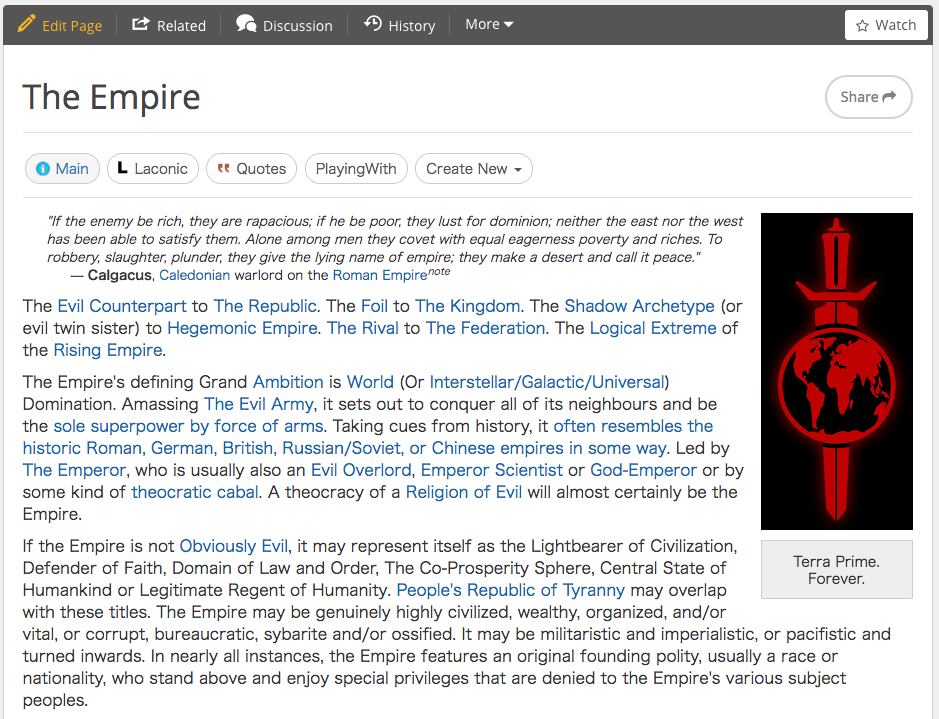
\includegraphics[height=5in]{evilEmpire.png}}
\caption{A screenshot of the ``The Empire'' wiki page from TV Tropes} \label{fig:evil-empire}
\end{figure}

Figure~\ref{fig:evil-empire} shows a screenshot of the ``The Empire'' page on the
website. It clearly shows the description of the trope at the top of the page,
and there are also instances of its use across different media at the bottom.

Tropes can also describe character archetypes. For example, this is how TV
Tropes describes \emph{Anti-Hero} characters:

\begin{quote}
An Archetypal Character who is almost as common in modern fiction as the Ideal Hero, an antihero is a protagonist who has the opposite of most of the traditional attributes of a hero. They may be bewildered, ineffectual, deluded, or merely apathetic. More often an antihero is just an amoral misfit. While heroes are typically conventional, anti-heroes, depending on the circumstances, may be preconventional (in a "good" society), postconventional (if the government is "evil") or even unconventional. Not to be confused with the Villain or the Big Bad, who is the opponent of Heroes (and Anti-Heroes, for that matter).
  \end{quote}

TV Tropes further clarifies that there are subdivisions of
Anti-Hero, depending on just how evil or cynical the character is. Batman, for
example, would be a highly cynical Anti-Hero who is nevertheless morally good.

Shakespeare's Macbeth is a character who becomes more and more of an evil Anti-Hero, until he is too morally evil
to still be a Hero and instead becomes a Tragic Villain.

Tropes can be very specific, referring to individual lines of dialogue.
One example is ``We Will Meet Again'':

\begin{quote}
The standard phrase when the villain finds that he has been defeated by the heroes and there is no point in staying around with the immediate Evil Plan foiled.
\end{quote}

Tropes can also be very abstract, referring to particular genres, types of
story, or events in a story that move the action forward. Other than the
previously mentioned ``Hero's Journey'' and ``The Empire'' tropes, another
example could be the ``Hilarity Ensues'' trope:

\begin{quote}
Actions that are dangerous or illegal often lead to injury, arrest, job dismissal, expulsion from school, deportation, or other dire consequences. Thankfully for our fictional friends, both the Rule of Cool and the Rule of Funny keep them safe (the latter more prominently).
\end{quote}

\emph{Metatropes} are tropes about tropes, often intended as a knowing wink to
the trope-savvy audience. One such example is ``Lampshade Hanging'', which TV
Tropes describes as:

\begin{quote}
...the writers' trick of dealing with any element of the story that threatens the audience's Willing Suspension of Disbelief, whether a very implausible plot development, or a particularly blatant use of a trope, by calling attention to it and simply moving on.
\end{quote}

In fact, even if an audience is unaware of the concept of tropes, they may be aware
of the recurring patterns and themes that tropes describe. This enables
genre-savvy writers (especially postmodernists such as Brecht and Vonnegut) to play with the audience's
expectations. Ways to do this with tropes could include \emph{inversion}
(reversing the trope),
\emph{subversion} (making it look like the trope will happen, but then not using
it after all), \emph{parody} (using the trope in an over-the-top, exaggerated
manner) and \emph{deconstruction} (using the trope in a straightforward manner,
but in way which forces the audience to analyse the trope itself).

Take, for example, the well-known ``The Butler Did It'' trope from murder
mystery stories, where the butler of the house is revealed to be the murderer at
the end of the story. TV Trope describes ways that an author could ``play'' with this trope:

\begin{itemize}
  \item \textbf{Subvert} it: The butler is the prime suspect at the beginning, and is later found innocent.
  \item \textbf{Invert} it: The butler is the victim. Or the butler solved the crime. Or every suspect except the butler was part of the crime.
  \item \textbf{Parody} it: Butlers could learn their trade at butler college where they are taught cleaning, cooking, and murdering.
  \item \textbf{Deconstruct} it: The butler is a revolutionary serial killer, who purposely takes jobs as butlers to murder his rich masters. All the unfortunate implications of class warfare that this suggests are brought up and discussed.
\end{itemize}

Many other examples of using tropes in this way can be found on the ``Playing
with a Trope'' page of the TV Tropes website~\citep{playing-tropes}.

\begin{figure}[p!]
\centerline{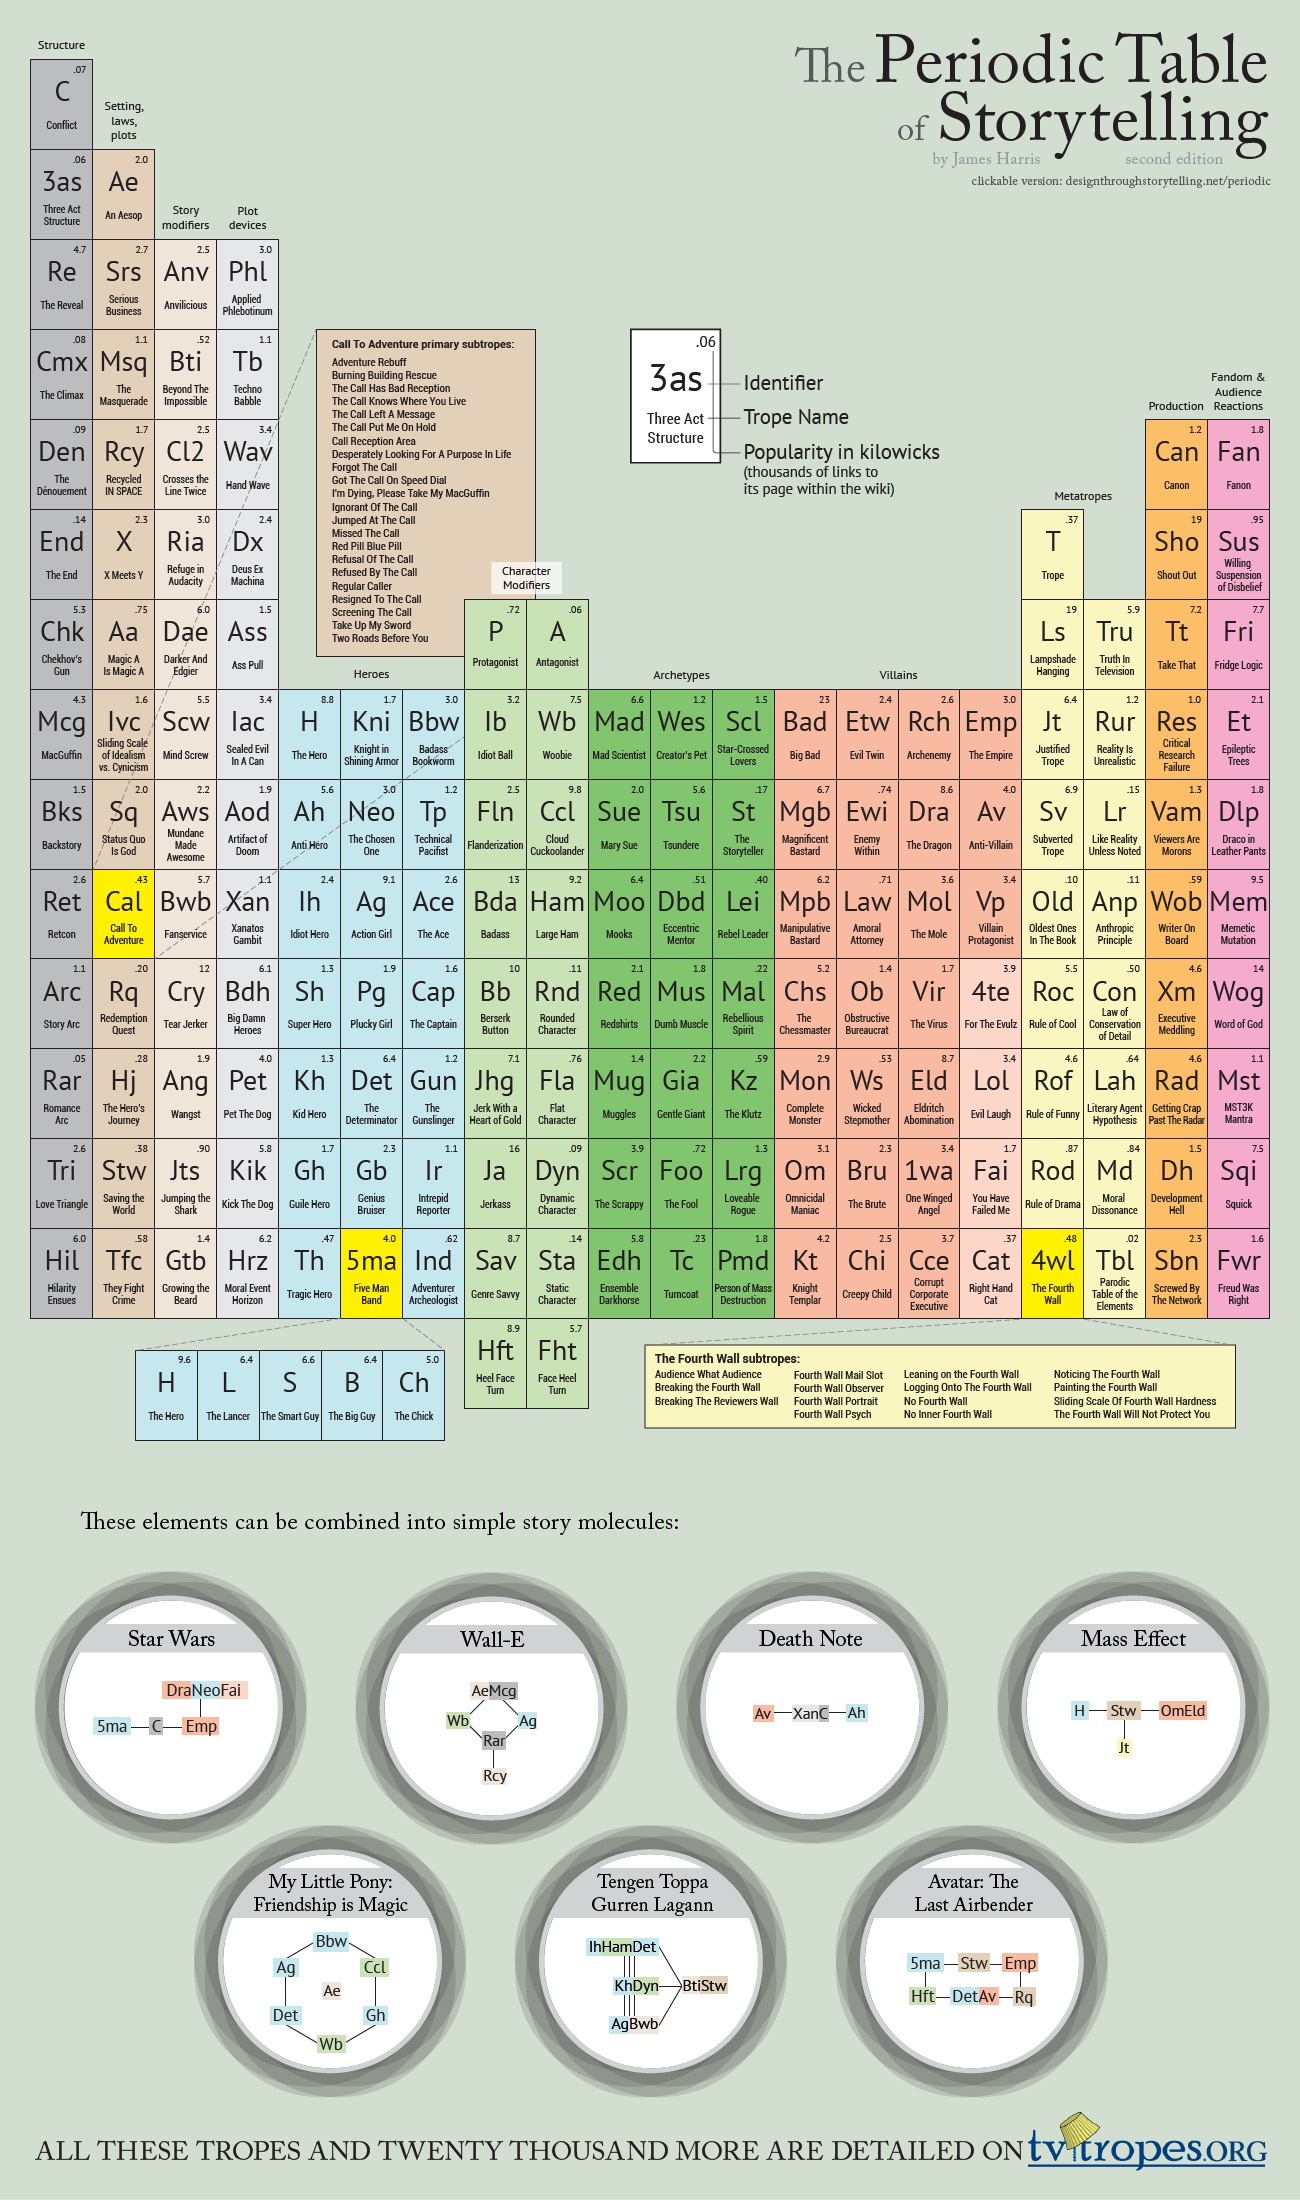
\includegraphics[height=0.9\textheight]{periodicTable.png}}
\caption{The ``Periodic Table of Storytelling'', original by James Harris
  (http://jamesharris.design/periodic/), poster format by Deviant Art user Dawn
  Paladin (http://dawnpaladin.deviantart.com/art/The-Periodic-Table-of-Storytelling-Second-Edition-425816342)} \label{fig:periodic-table}
\end{figure}

\begin{figure}[t!]
\centerline{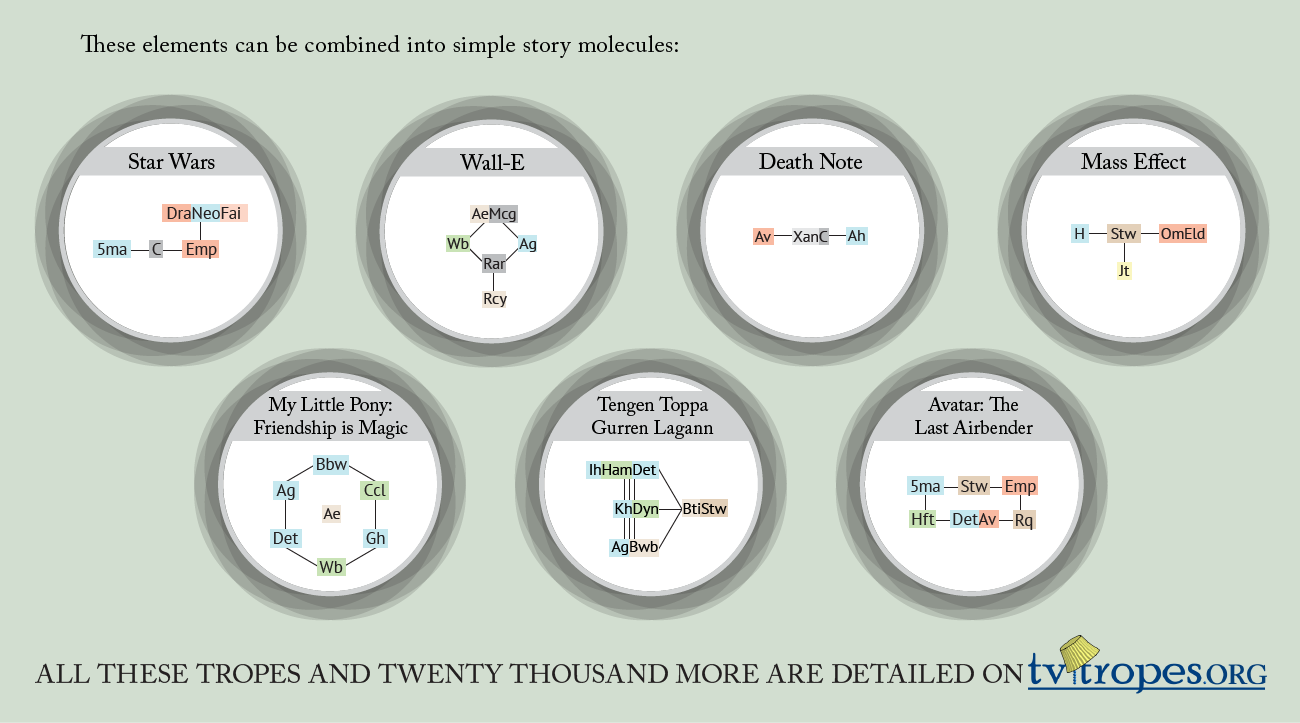
\includegraphics[width=\textwidth]{periodicExamples.png}}
\caption{Example ``Molecules'' from the ``Periodic Table of Storytelling'', original by James Harris
  (http://jamesharris.design/periodic/), poster format by Deviant Art user Dawn
  Paladin (http://dawnpaladin.deviantart.com/art/The-Periodic-Table-of-Storytelling-Second-Edition-425816342)} \label{fig:periodic-examples}
\end{figure}

A large and highly active community of users and contributors exists around TV
Tropes. In addition to creating content for and curating the content on the
website, they also work to create useful ways to visualise the usage of tropes
in stories. For example, The Periodic Table of
Storytelling~\citep{periodicTableOfStorytelling} is a visualisation of tropes as
``elements'' in the ``molecules'' of a story. The table itself
(Figure~\ref{fig:periodic-table}) arranges the tropes into different ``groups''
according to the part of a story that they operate on. The leftmost groups
describe the story as a whole, describing:

\textbf{Story structure:}
\begin{itemize}
  \item Three Act Structure
  \item MacGuffin
  \item Chekov's Gun
\end{itemize}

\textbf{Story Modifiers:}
\begin{itemize}
  \item Darker and Edgier
  \item Tear Jerker
  \item Jumping the Shark
\end{itemize}

\textbf{Plot Devices:}
\begin{itemize}
  \item Hand Wave
  \item Techno Babble
  \item Xanatos Gambit
\end{itemize}

In the centre of the table are different types of character such as:
\textbf{Heroes:}
\begin{itemize}
  \item Anti Hero
  \item Action Girl
  \item The Gunslinger
\end{itemize}

\textbf{Archetypes:}
\begin{itemize}
  \item Mad Scientist
  \item The Fool
  \item Loveable Rogue
\end{itemize}

\textbf{Villains:}
\begin{itemize}
  \item Evil Twin
  \item The Empire
  \item Obstructive Bureaucrat
\end{itemize}

The right third of the table contains self-referential tropes such as:

\textbf{Metatropes:}
\begin{itemize}
  \item Lampshade Hanging
  \item Subverted Trope
  \item The Fourth Wall
\end{itemize}

\textbf{Fandom and Audience Reactions}
\begin{itemize}
  \item Fanon
  \item Fridge Logic
  \item Freud Was Right
\end{itemize}

The story is then visualised as a molecule composed from tropes, linked together as
atoms, as shown in the various examples in Figure~\ref{fig:periodic-examples}.

By showing tropes as ``atoms'' that can be rearranged and combined into
different ``molecules'', this visualisation demonstrates our core idea of their use as reusable
story components, but the ``molecule'' metaphor is unsatisfactory for a couple of
reasons. Firstly, linking tropes together as atoms in a molecule does not
communicate the different levels of abstraction at which tropes operate.
Considering that our main purpose for choosing tropes as our method of
describing narrative components, this means that the ``molecule'' metaphor used
by the author does not match our intentions. The
``Hero's Journey'' trope, for example, would describe the narrative arc as a
whole, while the ``Comeuppance'' trope would describe just a single scene in the
story. The metaphor is also not ideal because it presents unrelated tropes
together in a story with no indication of which part of a narrative they affect.
A ``scoundrel sidekick'' could be linked together with a ``breaking the fourth
wall'' trope, even though one trope relates to a certain character, and the
other may describe a single line of dialogue or action that occurs at a specific
point in the story. In this visualisation, a trope that describes something as
significant as the structure of the entire story would carry the same weight as
a short event that occurs just once in the entire story. The arrangement and linking of the tropes in the example molecules is also
quite arbitrary. The examples given on the \emph{periodic table} web site form
interesting shapes, but do not follow a consistent logic. In the \emph{Star
  Wars} molecule, for example, the ``Five Man Band'', ``Conflict'' and ``The
Empire'' tropes are linked in a straight line suggesting a linear sequence, but
three further tropes (``The Dragon'', ``The Chosen One'' and ``You Have Failed
Me'') are all linked to the ``The Empire'' trope in the molecule. While ``The
Dragon'' refers to the Death Star in the movie, the ``The Chosen One'' trope is
more closely linked to Luke Skywalker's Hero role. The ``You Have Failed Me''
trope refers to a specific scene where villain Darth Vader punishes an
under performing henchman with choking. It is not clear why the creator decided
to link these specific tropes to the ``The Empire''
trope. This illustrates that such planar structures are insufficient to capture
anything but the simplest stories.

Similarly, in the \emph{GhostBusters} example, the ``Five Man Band'' and ``Mad
Scientist'' tropes appear together in the same ``atom'', which are linked to
``Sealed Evil in a Can'' and ``Hilarity Ensues''. Again, it is not clear why
those particular tropes are arranged together into the same atoms, or why they
are linked together in this way. The most likely explanation is that this
visualisation of the way that tropes link together in a story is not intended as
a formal system for trope visualisation, and is merely a proof-of-concept work.

Working from the ideas presented in this visualisation, we develop our concept of tropes as
logical, reusable components for the formal description of stories. 

% TODO rip the whole bit from the lit review? Consider it at least
\section{Why Use Tropes?}
% Write about ability to abstract, give story examples vs Propp
% This is pretty much covered in the lit review

Returning to the shortcomings of existing narrative formalisms we describe in
section~\ref{sec:litrev-discussion}, we now describe how tropes are suitable for use
as a narrative formalism that is able to overcome these limitations.

\subsection{A Means of Abstraction}
\label{sec:abstraction}
Most tropes form a hierarchy, with parent tropes such as the
\emph{Quest} containing child tropes such as \emph{Redemption Quest},
\emph{Sidequest} or a \emph{Quest for Identity}. This hierarchy arises from
story authors adding nuance to existing narrative archetypes through adaptation.
This is often achieved by mixing different tropes together. For example, a
``child'' trope of \emph{The Hero's Journey} could be \emph{The Anti-Hero's
  Journey}, combining the \emph{Anti-Hero} trope with the classic \emph{Hero's
  Journey} trope.
These child-tropes inherit some
of the characteristics of their parents, but add subtle or major changes. For
example, a \emph{Quest for Identity} follows the \emph{Quest} format, but is
constrained so that the item that is the subject of the quest is the hero's own
identity. This resembles the object-oriented programming mechanism of delegation, so one can imagine using
such a process to avoid duplication of effort when authoring new tropes by only
expressing how a trope differs from its parent.

\begin{figure}[!t]
\centerline{
\includegraphics[height=1.5in]{freytag.png}}
\caption{Freytag's Pyramid} \label{fig:freytag}
\end{figure}

Another method of abstraction is the embedding of sub-tropes as parts of
parent tropes. This is how tropes can be defined and then re-used inside stories: by allowing any
trope to be a component that can be dropped inside any other trope.
The example we described in Section~\ref{sec:litrev-discussion}
describes how the ``Quest'' trope could form one part of a larger trope
such as the ``Hero's Journey''. Another example of this would be the
\textbf{Three Act Structure} (also known as Freytag's Pyramid) shown in Figure~\ref{fig:freytag}, which describes the shape of a
story in terms of rising and falling levels of drama. This could be split into
five (or perhaps more) sub-tropes:

\begin{enumerate}
  \item \textbf{Exposition}: The setting of the scene, providing any background
    information that is relevant to the story.
  \item \textbf{Rising Action}: A series of event drive the story forward, each
    increasing in dramatic intensity.
  \item \textbf{Climax}: The turning point of the story. Some fateful event
    occurs as a result of the rising action, which could be a battle between the
    hero and the villain, for example.
  \item \textbf{Falling Action}: The consequences of the climax play out, and
    the story shows how the characters are affected.
  \item \textbf{Denouement}: This is the final resolution, where all the ``loose
    ends'' of the story are tied up.
\end{enumerate}

This means that if we already have trope definitions for the ``Exposition'',
``Rising Action'', ``Climax'', ``Falling Action'' and ``Denouement'' parts of a
story, and want to create a ``Three Act Structure'' trope, we can simply express
it in the following way:

\begin{enumerate}
  \item The ``Exposition'' trope happens
  \item Then the ``Rising Action'' trope happens
  \item Then the ``Climax'' trope happens
  \item Then the ``Falling Action'' trope happens
  \item Then the ``Denouement'' trope happens
\end{enumerate}

Returning to the concept of ``story structure'' described in
section~\ref{sec:structure}, we can use the ``subtropes'' we just identified to
define other ``story shapes'' as described by~\citet{vonnegut2009palm}. For example, the ``man
in hole'' story shape described in Section~\ref{sec:structure} could simply be described as a rearrangement of the
three-act structure:

\begin{enumerate}
  \item The ``Exposition'' trope happens
  \item Then the ``Falling Action'' trope happens
  \item Then the ``Nadir'' trope happens
  \item Then the ``Rising Action'' trope happens
  \item Then the ``Climax'' trope happens
  \item Then the ``Denouement'' trope happens
\end{enumerate}

Note that we added an additional trope, the ``Nadir'' trope to describe the
lowest point in the story. Otherwise, the rest of the story ``shape'' is easily
described in terms of tropes that we have defined already.

The fact that we can describe an abstract trope such as ``man in hole'' in terms
of more specific tropes addresses one of the shortcomings of the Periodic
Table's molecule model of tropes from Figure~\ref{fig:periodic-examples}: that
all tropes have equal weight in a story. Though the above example only describes
how these sub-tropes may be sequenced within their parent trope, they may also
be arranged as branching alternatives, so that either \emph{Trope A} \textbf{or}
\emph{Trope B} occur. This is discussed further in Section~\ref{sec:branch-code}.

This re-use of existing trope definitions saves us the time and effort of the wasteful duplication of the steps
already described within them. This is why abstraction is such a powerful
and useful concept: it allows us to break down complicated stories into a series
of smaller sub-stories, rather than having to describe the whole thing in one go.

\subsection{Conceptually Simple}\label{sec:tropes-simple}

Most story authors are already familiar with the concept of tropes. In order to
evaluate the suitability of their use for the description of narrative
components, we presented a preliminary version of our trope-based TropICAL programming
language (described in Chapter~\ref{cha:tropical}) for story authoring to the Oxford and London Interactive Fiction meetup group.

After a brief presentation on the concept of tropes and how we intend to use
them to create an authoring system for interactive narrative, participants were
given a questionnaire with the purpose of discovering their familiarity with
tropes, as well as finding out how suitable they thought tropes would be as a
new kind of formalism for narrative components.

There were 18 responses to the questionnaire. The questions and responses are
listed in Appendix~\ref{appendix:questionnaire}. The fact that all of the interactive fiction authors and games developers were
already familiar with the concept of tropes demonstrates that they are
conceptually simple enough for non-programmers to understand. Not only that, but
most of them were already familiar with the TV Tropes website. This meets our
requirement that authors should be able to create story components without
having to learn an unfamiliar set of concepts such as those used by~\citet{propp1968morphology}
or~\citet{lehnert1981plot}, which can only be discovered through reading
academic books and papers.

\subsection{A Library of Re-usable Examples}

One of the major strengths of Propp's system~\citep{propp1968morphology} is that
the \emph{morphology} is not only a theory: it is also a library of 31 story functions
that can be put together by story authors to create a narrative. The authors
need not create their own story functions, they can simply use the ones that
Propp has already created for them.

Though the TV Tropes website does not contain formal definitions of tropes, it
can be used as a resource on which to base the authoring of tropes in our system.
In addition, it grants authors the flexibility to create their own tropes which are not already listed on the
TV Tropes website.

TropICAL, our domain-specific programming language for trope-oriented story
authoring, aims to simplify the authoring of story tropes for non-programmer users.
In the same vein as Inform 7~\citep{reed2010creating}, our language uses a
constrained natural language syntax. Further details are described in
Chapter~\ref{cha:tropical}, where we describe the language in detail. In the same manner as a wiki, once a number of authors have contributed tropes,
it could offer the capacity to be a library of reusable tropes for future authors to use in
their stories.

To summarise: tropes have the potential to be a useful model to use for story
components, as they fulfil the criteria we lay out in
section~\ref{sec:litrev-discussion}:

\begin{itemize}
\item They provide a \emph{means of abstraction} through subtropes as well as parent and child
  tropes.
\item They are \emph{conceptually simple} for authors to learn, given that
all the authors in our preliminary study with the London Interactive Fiction
Meetup group are already familiar with them.
\item The TV Tropes website is a useful resource that can be used to aid the
  creation of a \emph{library of re-usable examples}.
\end{itemize}

% \section{Using Tropes with Modal Logic}
% In section~\ref{sec:pjexample}, we described the ``sausages'' scene from
% \emph{Punch and Judy} by combining Propp's story functions with modal operators
% to create Kripke structures to visualise the paths through the scene. In order
% to compare the expressiveness of tropes as a story formalism, this section
% describes the same scene, but instead using tropes in place of Propp functions.

% ACTUALLY DO THIS!


% \section{TropICAL: a DSL for Tropes} % 1
% \label{sec:tropical}

% We propose \tropical\ (the TROPe Interactive Chronical Language) as a DSL for describing tropes in a constrained natural language, which we compile to InstAL~\citep{cliffe2007specifying}, through which process we capture the events that can occur and the consequent state changes, and from which a model is constructed in ASP.  The model, when given an event trace, delivers the evolution of the trope state, including crucially, the addition or removal of permission associations between actors and actions and the addition of obligations as consequences of actors' actions.  The syntax of \tropical\ is heavily influenced by the Inform 7~\citep{reed2010creating} language for interactive fiction, with the tropes being expressed in constrained natural language mostly conforming to Attempto Controlled English (ACE)~\citep{fuchs1996attempto}. \tropical\ shares similar aims to Inform~7 in that it aims to make interactive fiction authoring accessible to non-programmer story authors, however its focus is on authoring and combining tropes written in terms of roles, in contrast to complete stories in terms of actual characters. This section describes the syntax and semantics of \tropical, as well as sketching its compilation to InstAL.

% The features of our trope description language are designed to be able to express the events, permissions and obligations of social institutions while addressing the shortcomings of planner and drama manager-based approaches:

% \begin{enumerate}[R1.]
% \item\label{perms} A way to express what certain characters are \textbf{permitted} to do at a given time.\footnote{An alternative approach would be to specify prohibitions, such that anything not prohibited is permitted, whereas we currently specify permissions, such that anything not permitted is prohibited.  This latter convention is the default semantics of InstAL, it is however straightforward from a technical point of view to adopt the alternative, as demonstrated in \citet{DBLP:conf/atal/KingLVDJPR15}.}
% \item\label{obls} A way to express \textbf{obligations} on characters, with \emph{deadlines} and \emph{penalties} if the obligations are not fulfilled.
% \item\label{state} A way to describe the state of a character or object at a
%   given point in the story.
% \item\label{seqs} A way of \textbf{sequencing} events in a trope.
% \item\label{conds} A way to express \textbf{conditionals}, so that some events may occur only if others have.
% \item\label{branches} A way to have \textbf{branches} in a trope, so that only one of two events may occur.
% \item\label{embed} A way to \textbf{embed} sub-tropes inside of parent tropes.
% \end{enumerate}
% Requirements~R\ref{perms} to~R\ref{seqs} allow \tropical\ to describe the
% permissions, obligations and sequences of events that occur in social
% institutions, while R\ref{conds} and~R\ref{branches} add the ability to specify
% alternative paths through a story, as planner-based systems are able to do when
% combined with formalisms such as Propp's. Finally, requirement~R\ref{embed}
% enables us to nest tropes to go beyond the capabilities of structuralist
% formalisms of narrative, addressing the limitations described in the ``Related
% Work'' chapter of this thesis (Chapter~\ref{cha:literature-review}). The TropICAL language satisfies these technical requirements, while being easy to learn for non-programmers, especially those familiar with the Inform 7 language (as is supported by the evaluation). It supports the expression of the above features in the following ways: 

% % Replace with ``hostage situation''?
% \begin{figure}[!t]
% % \begin{lstlisting}[float=t!,caption={The ``Hero's Journey'' trope in TropICAL},label=lst:hero]
% \begin{lstlisting}[showstringspaces=false]
% "The Hero's Journey" is a Trope where:
%   The Hero is at Home
%   Then the Hero meets the Dispatcher
%   Then the "Quest" trope happens
%   Then the Hero returns Home
% \end{lstlisting}%
% \caption{The ``Hero's Journey'' trope in TropICAL\label{lst:hero}}
% \medskip
% % \begin{lstlisting}[float=t!,caption={The ``Evil Empire'' trope in TropICAL},label=lst:evil]
% \begin{lstlisting}[showstringspaces=false]
% "The Evil Empire" is a Trope where:
%   The Villain has an Empire
%   The Empire is a Weapon
%   The Villain has a Victim
%   The Villain may kill the Victim
%   The Villain may kill the Hero
% \end{lstlisting}%
% \caption{The ``Evil Empire'' trope in TropICAL\label{lst:evil}}
% \medskip
% % \begin{lstlisting}[float=t!,caption={The ``Quest'' trope in TropICAL},label=lst:quest]
% \begin{lstlisting}[showstringspaces=false]
% "Quest" is a Trope where:
%   Then the Hero must go to the Land Of Adventure before the Villain kills the Victim
%     Otherwise, the Story ends
%   When the Hero goes to the Land Of Adventure:
%     The Hero may rescue the Victim
%     The Hero may kill the Villain
%       Or the Villain may escape
% \end{lstlisting}
% \caption{The ``Quest'' trope in TropICAL\label{lst:quest}}
% \end{figure}

% \begin{compactdesc}
% % \subsection{Permissions}
% \item[Permissions:]
% Permissions on characters can be described by making statements in the simple present form, such as ``The Hero finds a weapon''. When compiled to InstAL code, these statements are equivalent to giving a character permission to do something. In this case, the Hero would have permission to find a weapon at that point in the trope.
% The reason that this statement is translated to a permission is so that character agents can at any time have multiple permitted actions from several active tropes. It makes sense to make permission the ``default'' norm, rather than obligation, to allow the agents as much freedom as possible within the constraints of the story. If an author wants to make sure an agent carries out a particular action, they would specify it as an obligation instead (``The Hero \emph{must} find a weapon'').

% % \subsection{Obligations}
% \item[Obligations:]
% Figure~\ref{lst:quest} shows an example of an obligation with both a deadline and a violation event (both of which are optional). This obligation states that the hero must go to the Land of Adventure before the villain kills the victim, otherwise the story ends. In this case, the story ending is a particularly harsh penalty for the violation of the \emph{Quest} trope. Alternative violation events could be reduction of the hero's health, or the death of the victim.

% \item[State:]
% There are certain properties of each character or object in a story that will hold (or not
% hold) at different points of time. For example, we want to be able to keep track
% of the physical location of each character or object, what items a character possesses, or the
% state of their health, for example. There are two keywords that we use to
% express the state of a character: \emph{is} and \emph{has}.

% For example, we can say that:
% The \emph{sword} \textbf{is} in the \emph{castle}.
% The \emph{hero} \textbf{is} at \emph{home}

% Or:
% The \emph{hero} \textbf{has} the \emph{sword}.
% The \emph{villain} \textbf{has} the \emph{macguffin}.

% These statements would be used to initiate and terminate fluents in their
% corresponding institutions. The state of the story will progress according to
% the combination of fluents that hold at a particular time.

% % \subsection{Sequencing}
% \item[Sequencing:]
% As well as specifying permissions and obligations, it is frequently necessary to be able to express that certain events can only occur in a certain order. The \emph{Then} keyword means that the succeeding statement can only occur once the previous event has occurred. This is the means of implementing the \emph{phases} described in the ``Ordering Events in Tropes'' part of this section. In the \emph{Hero's Journey} (Figure~\ref{lst:hero}) example, the Hero only has permission to return home (line 5) once everything in the \emph{Quest} trope has happened (Figure~\ref{lst:quest}).
% In some tropes, such as the \emph{Evil Empire} trope (Figure~\ref{lst:evil}), the permissions and obligations described do not always need to occur in a certain sequence. In this case the trope serves the purpose of describing certain themes and characters in a part of a story, or events that may occur at any time, rather than in a specific order. The \emph{Evil Empire} trope only needs a villain with an empire to be present to fight the hero, so all of its permissions and obligations will apply from the beginning of the story.

% % \subsection{Branching}
% \item[Branching:]
% Tropes may also contain branching paths where one or more events may take place. This is expressed in TropICAL with the \emph{Or} operator. Lines 6 and 7 of the \emph{Quest} trope in Figure~\ref{lst:quest} express two alternatives: the Hero may kill the Villain or the Villain may escape. In this case, both permissions will hold at the same time, but both will be terminated once either permitted event has occurred. This makes it impossible for both events to happen in the story.

% % \subsection{Conditionals}
% \item[Conditionals:]
% Conditionals are another way to create branching paths in a narrative, by allowing certain actions to occur if a particular trope state is reached. For this purpose we add the \emph{When} keyword, to express that when a specified state or event occurs, then some norms will be activated. In our \emph{Quest} example, we see an example of this on line 4, stating what the hero may do once in the Land of Adventure. This is similar to the ``Simple Present Statement'' example, except for the addition of the \emph{When} keyword. In much the same way, the statement after the \emph{When} keyword is a permission that holds on a character during the trope, except that it is also used to describe the consequences of certain events occurring. In this case, it states that when the Hero goes to the Land of Adventure, they may either kill the Villain, or the Villain may escape.

% % \subsection{Embedding Tropes Within Tropes}
% \item[Embedding Tropes Within Tropes:]
% Tropes can be embedded inside other tropes by simply writing \emph{The X trope happens}.
% Line 4 of the \emph{Hero's Journey} trope (Figure~\ref{lst:hero}) shows an example of embedding one trope inside another. In this case, the \emph{Quest} trope occurs at a certain point in the \emph{Hero's Journey}, once the hero has met the dispatcher character. Because this is sequenced using the \emph{Then} keyword, these events must occur in the specified order, and the norms described in the \emph{Quest} trope cannot hold until the specified point in the trope. However, if the \emph{Then} keyword is omitted (\emph{The ``Quest'' trope happens}), this means that the norms contained inside the embedded trope apply from the start of its containing trope. In our example, this would mean that the Hero would be free to embark on a quest at any time, rather than waiting to first meet a dispatcher character.

% Rather than compiling all the tropes into one institution, they are compiled
% into separate institutions and coordinated using a ``bridge'' institution. This
% technique, described by~\citep{bath45254}, allows institutions to generate
% events inside of other institutions while keeping each one separate. The
% cross-institution event generation logic is described in the ``Institutional Bridges''
% section of the next chapter (Section~\ref{sec:bridges}).
% \end{compactdesc}

This chapter has described the concept of tropes, breaking down several examples
and describing them as normative institutions. We then returned to our
\emph{Punch and Judy} example to describe a scene in terms of tropes rather than
Propp functions. 
% high-level overview of the features of the language we have created (named \emph{TropICAL}).

The next chapter describes the design and implementation of \emph{TropICAL}, our
domain-specific language for describing tropes. TropICAL compiles controlled
natural-language trope descriptions to formal representations in terms of InstAL
institutions. After discussing requirements and design rationale, the chapter
lists annotated snippets of TropICAL code for example tropes and their
corresponding translations to \emph{InstAL}.

\chapter{TropICAL: A Language for Story Tropes}
\label{cha:tropical}
% TODO: describe pipeline
% parse -> data structure -> InstAL -> AnsProlog

This chapter describes the design and implementation of TropICAL (the TROPe
Interactive Chronical Action Language), our Domain Specific Language for
story tropes. The purpose of this language is to allow for the
creation of interactive narratives through the description of tropes in a
constrained natural language. The tropes created through the language are
designed to be reusable components that can go into a ``library'', from which
story authors can choose the tropes they wish for the particular story that they
are creating.

The motivation for the creation of TropICAL is the lack of any methods of
creating agent-based interactive narrative that are suitable for non-programmers
to use. Inform 7~\citep{reed2010creating} enables non-programmers to create
interactive fiction, but not in a way that can be integrated into a multi-agent
system.
The systems described in the literature review in
chapter~\ref{cha:literature-review}, such as those using the Mimesis
architecture~\citep{young2004architecture}, a drama manager and planner such as
in Fa\c{c}ade's system~\citep{mateas2003faccade}, or linear logic as in Ceptre's
system~\citep{martens2015ceptre}, all require the story author to be familiar with
planner-based systems or the description of formal logics. The purpose of
TropICAL is to greatly reduce the barrier to the creation of interactive stories
with intelligent agents by allowing authors to describe the components of their story using constrained
natural language. These story components integrate with a multi-agent system by
describing the constraints on the actions of each character agent in the story,
telling each agent what they are permitted and obliged to do at any point in the
narrative.

Many authors using our system should not even need to
write their own tropes using TropICAL, and will instead simply select the tropes
that they need for their story from a pre-created ``library'' of tropes. This
process is facilitated through the ``StoryBuilder'' user interface described in
Chapter~\ref{cha:storybuilder}

Our TropICAL language design is as follows:

\begin{itemize}
  \item It is based around the idea of using \emph{story tropes} as reusable
    components that can be combined to create stories
  \item It uses \emph{controlled natural language} to describe these tropes
  \item The controlled natural language is then parsed and compiled to a data
    structure that describes the formal features of each trope
  \item The intermediate data structure is then used to generate InstAL code
  \item The InstAL code is compiled to AnsProlog, an Answer Set Programming
    language
  \item The AnsProlog code is then run through
    \emph{clingo}~\citep{gebser2011potassco}, an answer set solver, to generate
    all the possible sequences of events that can occur in the story.
\end{itemize}

This chapter begins by describing TropICAL's constrained natural
language syntax in Section~\ref{sec:t-constrained}.
Section~\ref{sec:t-requirements} explores the use cases for our language, deriving
a set of requirements from them. Based upon these requirements, the features and
design of the language are described in Section~\ref{sec:language-design}.
The translation of TropICAL to InstAL code is demonstrated in Section~\ref{sec:t-codegen}, with samples of generated InstAL
institutions, Answer Set
generation (section~\ref{sec:t-asp}), constraints
(section~\ref{sec:t-constraints}), and output traces (section~\ref{sec:example-traces}). Finally, we show its extension for
the description of legal policies (section~\ref{sec:t-legal}). The chapter
concludes with a summary in Section~\ref{sec:tropical-summary}, describing how
some requirements from Section~\ref{sec:requirements} were met, while others are
addressed through the \emph{StoryBuilder} tool described in Chapter~\ref{cha:storybuilder}.


\section{Controlled Natural Language Syntax}
\label{sec:t-constrained}
% DONE intro: 1
% DONE describe ACE: 2
% DONE describe Inform 7: 2

TropICAL uses a \emph{Controlled Natural Language} syntax (also referred to as
\emph{Constrained Natural Language}), meaning that it superficially
resembles natural English, but is only a subset of the full language.

There are two types of Controlled Natural Language (CNL). The first type are \emph{naturalistic} languages
such as ASD Simplified Technical English~\citep{asd2007simplified}, designed to
be used in documentation for technical industries such as aerospace or defense,
or Ogden Basic English~\citep{ogden1944basic}, a simplified language for teaching
English as a second language. This type of Controlled Natural Language merely
describes a subset of the parent language. The other type of CNL are
\emph{formalistic}, with a formal
syntax and semantics, which can be mapped to rules in other formal languages
such as first-order logic. Attempto Controlled English~\citep{fuchs1996attempto}
is an example of this formal type of CNL, and the one which forms the basis of
our syntax for TropICAL.

\subsection{Attempto Controlled English}

Attempto Controlled English (ACE) is a controlled natural language that is also
a formal language, and was created by the University of Zurich in 1995. It is
still under development, with version 6.7 of the language announced in 2013. ACE
has been used in a wide variety of fields, such as software specifications,
ontologies, medical documentation and planning.

ACE's vocabulary has three components:

\begin{itemize}
  \item predefined function words
  \item predefined fixed phrases (\emph{there is}, \emph{it is false that}, ...)
  \item content words (nouns, proper nouns, verbs, adjectives, adverbs)
\end{itemize}

The Attempto Parsing Engine (APE) has a lexicon of content words, and users can
define their own content words. User-defined content words take precedence over
the built-in lexicon.

ACE's syntax is expressed as a set of construction rules (admissible ACE
sentence structures), with syntactically
correct sentences described as a set of interpretation rules, which contain the
actual semantics of the sentences.

The simplest ACE sentences follow a \emph{subject + verb + complements +
  adjuncts} structure:

\begin{lstlisting}
  A dragon sleeps.
  The sky is blue.
  A princess owns a castle.
  A king gives a sword to a knight.
\end{lstlisting}

In this structure, every sentence must have a subject and a verb. Sentences that
do not contain a verb are expressed with the \emph{there is} structure:

\begin{lstlisting}
  There is a kettle.
  There are 3 balls.
\end{lstlisting}

Details can be added to these sentences through the use of adjectives, and the
sentences can be joined together with the \emph{and} and \emph{then} keywords.

Other ways of modifying the sentences include \emph{negation}, adding
\emph{quantifiers}, or making the sentences \emph{interrogative} or
\emph{imperative}. We do not go into further details in this thesis, as we are
using ACE simply as an inspiration for our syntax, rather than following its
design entirely. For more details, see the ``ACE in a Nutshell''
page\footnote{Located at the following URL:
  \url{http://attempto.ifi.uzh.ch/site/docs/ace_nutshell.html}, accessed 20170826.} of its
documentation for an overview of the language~\citep{ace-nutshell}.

\subsection{Inform 7}
Besides ACE, the other main inspiration for TropICAL's syntax is the
\emph{Inform 7} language.

Inform is a programming language for the creation of Interactive Fiction (also
called \emph{text adventure games}). All versions of Inform generate
\emph{Z-code}, which is interpreted by the \emph{Z-machine} virtual machine for
interactive fiction.

The syntax of the language has changed multiple times since its creation in
1993. The version of the language that we are most interested in is Inform 7~\citep{reed2010creating},
which is its most recent incarnation. Prior to Inform 7, the language used
traditional programming models such as procedural and object-oriented paradigms.
With version 7, however, its creator Graham Nelson redesigned its
syntax completely to allow authors to create their stories using controlled
natural language, so that the experience of story creation became closer to that
of writing a book.

The simplest possible game authored with Inform 7 would be:

\begin{lstlisting}[showstringspaces=false]
"Hello World" by "I.F. Author"

The world is a room.

When play begins, say "Hello, world."
\end{lstlisting}

The above code simply describes the name of the game (``Hello World''), declares
that there is one room in the game, and sets the game to say ``Hello World'' to
the player when the game starts.

An extended example, Will Crowther's cave exploration simulation, would be
described like this:

\begin{lstlisting}[showstringspaces=false]
"Cave Entrance"

The Cobble Crawl is a room. "You are crawling over cobbles in a low passage. There is a dim light at the east end of the passage."

A wicker cage is here. "There is a small wicker cage discarded nearby."

The Debris Room is west of the Crawl. "You are in a debris room filled with stuff washed in from the surface. A low wide passage with cobbles becomes plugged with mud and debris here, but an awkward canyon leads upward and west. A note on the wall says, 'Magic word XYZZY'."

The black rod is here. "A three foot black rod with a rusty star on one end lies nearby."

Above the Debris Room is the Sloping E/W Canyon. West of the Canyon is the Orange River Chamber.
\end{lstlisting}

The ``Cave Entrance'' example above is just one scene from the game. The code
begins with a declaration of the ``Cobble Crawl'' room, followed by the
description that appears when the player enters it. The next line declares that
a wicker cage is in the room, which is an object that the player can interact
with. The sentence after the declaration is the description of the item that
appears when the player looks around the room (``There is a small wicker cage
discarded nearby.'').
The ``Debris Room'' follows the same format described above, with a ``black
rod'' item inside the room. The final line of code simply describes how the
rooms are arranged in the game, using words like ``above'' and ``west of''.

Although Inform 7 is not based directly on ACE, we can see many of ACE's
features in it. For example, it uses the same syntax for simple statements such
as \emph{X is a Y}. Most statements in the listing above are pairs of sentences,
with the first in each pair declaring the existence of an object or room, and
the second being an uninterpreted string that is printed out as the description
of the defined object.

Before version 7, Inform was already widely used as a language for the creation
of Interactive Fiction. Given its continued popularity after the switch to
a controlled natural language syntax\footnote{The Interactive Fiction Database
  at \url{http://ifdb.tads.org} (accessed 20170826) lists 1078 games created
  with Inform 6, and 914 created with Inform 7. Inform 6 has been in use since
  1996, Inform 7 since 2006.}, it appears that the new programming
paradigm is successful.

The wide adoption of Inform 7 by story authors with no other programming
experience motivates our decision to create a controlled natural language syntax
for TropICAL, our own trope-based programming language. The intended audience is
the same, so an additional benefit would be that story authors who can code with
Inform 7 would also be able to use TropICAL.

\section{Requirements}
\label{sec:t-requirements}
% TODO intro: 1
% TODO use cases: 2
% TODO requirements: 2
% TODO list features: 1
% TODO tech used: 1
% TODO relate features to the requirements: 2

The TropICAL language is designed to be used by authors of interactive
narratives, enabling them to easily describe the ``rules'' of a story through
tropes. It is designed to be used in interactive storytelling systems where
intelligent software agents are acting out the roles of the characters in the
story. These agents, through an architecture such as BDI (Belief, Desire,
Intention), have their own goals and plans for how to achieve those goals.
TropICAL does not assist in the authoring of these characters and their plans or
lines of dialogue. Instead, its purpose is to guide the actions of these
``character'' agents so that certain behaviours are suggested by the rules of the author's
story. TropICAL is designed to be used with a system where the character agents have
already been authored. It guides them by allowing the characters to know what
they are permitted and obliged to do according to the story. For a description of how this is
implemented in practice, see Section~\ref{sec:punchjudy} of
Chapter~\ref{cha:institutions}.

\subsection{Use Cases}
\label{sec:use-cases}

In order to design a set of tools that is suited to interactive story authors, we derive our set of requirements from specific use
cases. These use cases come from the user stories of three hypothetical users: Alice, Bob and
Charlie. In each case, we tell the user's story, highlighting their different
levels of technical experience, along with
their various needs for and ways of using tools for
interactive story creation.

\subsubsection{Alice}

Our first user story focuses on \emph{Alice}, a user with some programming knowledge and
specialist expertise in the field of intelligent agents:

\begin{quote}
  Alice is an interactive narrative researcher using the Jason intelligent agent
  framework to create the characters of a story. The story is a classic
  detective noir story, with a private investigator as the main character and
  several suspects, one of which is the killer. She has coded their behaviour
  and dialogue as a set of plans, which each agent will follow according to
  their beliefs, desires and intentions as they ``act out'' the story.

  Alice sets the simulation running, but sees that although the agents are interacting
  with each other as intended, there is no structure or sense of drama to the
  story. It merely seems to be one event happening after another.

  She decides to use the TropICAL framework to guide the actions of the
  character agents. The tropes that she chooses to describe her story are the
  ``Three Act Structure'', ``Chekov's Gun'', ``Murder Mystery'' and ``Rooftop
  Chase'' tropes. These tropes are used to not only give the story structure,
  but also to encourage the characters in it to behave in a way that makes the
  simulation ``feel'' like a murder-mystery genre novel.

  When using TropICAL, she selects the ``Three Act Structure'' and ``Chekov's
  Gun'' tropes from a pre-written library of tropes. However, she cannot find
  tropes that describe what a ``Murder Mystery'' story is, or what should happen
  in a ``Rooftop Chase'' scene. She creates these by writing her own tropes in TropICAL:

  \begin{lstlisting}[showstringspaces=false]
  ``Murder Mystery'' is a trope where:
    The Detective is a role
    The Killer is a role
    The Victim is a role
    The Killer kills the Victim
    The Detective investigates the Killer
    Then the Detective catches the Killer
      Or the ``Rooftop Chase'' happens

  ``Rooftop Chase'' is a trope where:
    The Detective is a role
    The Fugitive is a role
    The Rooftop is a place
    The Detective goes to the Rooftop
    The Fugitive goes to the Rooftop
    The Detective chases the Fugitive
    Then the Detective catches the Fugitive
      Or the Fugitive escapes
\end{lstlisting}
\end{quote}

From Alice's story, we can derive the following requirements:

\begin{enumerate}[{Alice} R1.]
\item She needs a system for describing stories that can be used with a
  multi-agent system framework such as Jason\label{req:alice1}
\item The system needs to direct the behaviour of the agents so that their
  actions fit within the description of a story\label{req:alice2}
\item She needs to be able to write and re-use story components that fit the
  theme of her story (in this case, ``film noir'').\label{req:alice3}
\item These story components must be able to express both sequences of events
  and diverging (``branching'') events\label{req:alice4}
\item She wants to be able to select existing story components from a library or database\label{req:alice5}
\item She also wants the ability to create her own story components and save
  them to the database\label{req:alice6}
\end{enumerate}

\subsubsection{Bob}

Our second hypothetical user, \emph{Bob}, has no technical expertise at all:

\begin{quote}
  Bob is a traditional story author interested in writing interactive narratives
  with branching plot lines. He has written a few stories in the style of the
  ``Choose Your Own Adventure'' books, using the traditional method of using paper and
  pen to write down the stories. He implements the story branches by labelling
  each scene with a name such as ``The Hero Sets Off on a Journey'', or ``The
  Villain Deceives a Victim'', and referring to them by name whenever a
  branching point occurs. For example, when the Hero of a story is tasked with a
  quest to complete, the decision could be to go to the ``Leave Home and Go on a
  Journey'' scene, or the ``Stay at Home and Avoid Adventure'' scene, which
  would be the names of scenes leading either to further choices, or the end of
  the story.

  While he is writing the story, he finds it difficult to keep a mental model of
  the whole plot, with all its branches, in his head. As he creates new choices
  and branching points in the story, he finds himself having to pin up notes on
  a board, and connect them with string.
  Frustrated, he searches for software to help him with the process of authoring
  non-linear stories, eventually finding a piece of software called ``Twine''.
  Twine's user interface uses the analogy of notes on a pinboard connected with
  string, the exact process he is used to. He quickly inputs the story he is
  working on into Twine, and it produces an HTML website with hyperlinks to
  pages representing the scenes of his story.
  Next, Bob wants to get more ambitious by abstracting away different parts of
  his story and re-using them in different places. He wants his story to be
  heavily quest-driven, with the player being given many different quests and
  missions over the course of the game. He decides that all of these quests
  follow a common pattern:

  \begin{lstlisting}[showstringspaces=false]
  The Hero is at Home
  Then the Hero meets the Dispatcher
  Then the Hero receives a Quest
  Then the Hero completes the Quest
    Or the Hero ignores the Quest
\end{lstlisting}

  In this case, the actual content of the ``Quest'' would change for each
  individual quest, but the way the player receives and embarks on the Quest
  remains the same. Bob wants to write this combination of nodes and branches
  once, and then re-use it as a single node labelled ``Quest''. Unfortunately,
  he finds no way to do this using Twine, and he is forced to copy and paste the
  existing nodes every time he wants to put a Quest into his story.
\end{quote}

Bob shares some requirements with Alice:

\begin{enumerate}[{Bob} R1.]
  \item He wants to be able to create story components with sequences of events
    and branching events\label{req:bob1}
  \item He wants to be able to save and re-use the components (to a database,
    for example)\label{req:bob2}
  \item He also wants the ability to create his own story components to add to
    the database\label{req:bob3}
\end{enumerate}

However, Bob also has some different requirements from Alice:

\begin{enumerate}[{Bob} R1.]
  \setcounter{enumi}{3}
  \item He needs to embed tropes inside other tropes (as ``sub-tropes'')\label{req:bob4}
  \item He needs to be able to visualise all of the story branches that result
    when one or more tropes are combined together\label{req:bob5}
\end{enumerate}

\subsubsection{Charlie}

Our final user, \emph{Charlie}, has technical expertise, and is also familiar with
existing research techniques for interactive narrative generation:

% Charlie needs to give agents autonomy to break away from the prescribed narrative
\begin{quote}
  Charlie is an experienced Interactive Narrative author that wants to
  automatically generate many of the small narrative details. By using
  intelligent agents to simulate the characters in the story, she hopes that
  their intelligence and autonomy will result in some surprising narrative arcs.

  First, she authors the character agents using the Jason library for
  intelligent agents. To do this, she must give them a library of plans to
  execute in order to carry out certain goals. At any moment in the story, each agent has a set of
  \emph{beliefs} about its environment, plans that they \emph{desire} to carry
  out, and plans that they \emph{intend} to execute.

  She sets the simulation running, but finds that the characters actions do not
  follow the structure of a story. She starts out by directing their actions using a planner-based system, but
  finds that the resulting stories don't make use of the agents' intelligence.
  The planner is simply telling the agents what to do, based on its goals. She
  thinks that this is fine most of the time, but nonetheless desires to
  occasionally see some unexpected (but plausible) actions from the characters.
  For example, if a character is close to finishing a plan to achieve a goal,
  she wants them to  choose to override what they are told to do by the director
  planner, and accept some penalty that comes with the violation of the story.

  She attempts to write this functionality into the agents' decision-making
  process, but this turns out to be too time-consuming, and she soon gives up.
  If only there were a better way.
\end{quote}

Charlie's only unique requirement is:

\begin{enumerate}[{Charlie} R1.]
  \item A way to describe the story such that the agents are told what to do
    next, but are able to break away from these commands when necessary.\label{req:charlie1}
\end{enumerate}

\subsection{Requirement Specification}
\label{sec:requirements}

Based on the use cases above (section~\ref{sec:use-cases}), we can create the
following requirements:

\begin{enumerate}[R1.]
  \item\label{req:agents} The software must be able to integrate into a
    multi-agent framework such as Jason (Alice R\ref{req:alice1})
  \item\label{req:direct} The system must direct the behaviour of agents to fit
    a story description (Alice R\ref{req:alice2})
  \item\label{req:components} The user must be able to write and re-use
    existing story components (from a library) (Alice R\ref{req:alice3}, R\ref{req:alice5} and R\ref{req:alice6}, Bob R\ref{req:bob2})
  \item\label{req:sequences} The components must be able to express sequences of
    events (Alice R\ref{req:alice4}, Bob R\ref{req:bob1})
  \item\label{req:branches} The components must be able to express branching
    (diverging) events (Alice R\ref{req:alice4}, Bob R\ref{req:bob1})
  \item\label{req:subtropes} The user must have the ability to nest existing
    components inside new components (Bob R\ref{req:bob4})
  \item\label{req:vis} The user must be able to visualise the branches of the
    story that result in the addition or modification of components to the
    story. (Bob R\ref{req:bob5})
  \item\label{req:norm} The story must tell the character agents what to do, but
    they should be free to break away from it in extreme circumstances, to add a
    degree of unpredictability (Charlie R\ref{req:charlie1})
\end{enumerate}

The next section describes the design of the TropICAL language, relating each
design decision back to these requirements derived from the use cases.

\section{Language Design and Features}
\label{sec:language-design}
In this section, we describe the main features of the TropICAL programming
language:

\begin{itemize}
  \item Entity Declarations (Section~\ref{sec:dec-code})
  \item Sequences of Events (Section~\ref{sec:seq-code})
  \item Obligations (Section~\ref{sec:obl-code})
  \item Branching Events (Section~\ref{sec:branch-code})
  \item Subtropes (Section~\ref{sec:subtrope-code})
\end{itemize}

% Each part of this section contains code samples to demonstrate the use and
% implementation of each language feature. Many of these samples are only extracts from
% full trope definitions in TropICAL, however. More extensive examples of trope
% definitions can be found in Appendix~\ref{appendix:tropes}.

This section begins by showing how the entities (roles, objects and places) of a
trope are defined by the author (Section~\ref{sec:dec-code}), then follows this with a description of how
these entities' actions are composed together to form sequences of events (Section~\ref{sec:seq-code}).
Normally, these events give the character entities \emph{permission} to perform
certain actions, so Section~\ref{sec:obl-code} shows how an author may
describe events that \emph{must} happen in the story through obliging characters
to carry out specific actions.
In cases where multiple story paths may be taken, TropICAL allows for the
description of alternative narrative branches, the syntax for which is described
in Section~\ref{sec:branch-code}. Finally, the means for creating trope
abstractions by embedding existing tropes into new ones is demonstrated in
section~\ref{sec:subtrope-code}.

\subsection{Entity Declarations}
\label{sec:dec-code}
A trope may contain three types of entities that take part in a trope:

\begin{itemize}
  \item Roles (characters acted out by the agents)
  \item Objects (items that are used or manipulated by the characters)
  \item Places (locations that the characters visit)
\end{itemize}

Before an author can use any characters, objects or places in their tropes, they
must first declare them at the top of the description file. For example, to declare
that the \emph{Hero} and \emph{Evil Villain} are character roles, one would write:

\begin{lstlisting}[label={lst:dec-roles}, caption={Role declarations}]
The Hero is a role
Evil Villain is a role
\end{lstlisting}

In TropICAL, the ``The'' at the beginning of role, object or place names is
optional. If the name of an entity begins with ``The'', the parser
omits it from the name. Also, entity names can consist of multiple words, as is
the case for the \emph{Evil Villain} character. However, each word in a name must
always start with a capital letter.

Similarly, to declare that our trope contains \emph{Sword} and \emph{Magic Potion} objects,
the author would write:

\begin{lstlisting}[label={lst:dec-objs}, caption={Object declarations}]
The Sword is an object
The Magic Potion is an object
\end{lstlisting}

Finally, \emph{Home} and \emph{The Land of Adventure} locations in the
trope are declared in the same way:

\begin{lstlisting}[label={lst:dec-places}, caption={Place declarations}]
Home is a place
The Land of Adventure is a place
\end{lstlisting}

Once the author has declared the entities of their trope at the top of the trope
definition, they are able to use them inside the events of the trope itself.

\subsubsection{Entity Instances}
\label{sec:entity-instances}
In cases where multiple characters fulfil the same role (a story could have two
hero characters, for example), or there are multiple objects or locations of the
same type, these entity instances can be declared separately. An example with multiple Heroes, Swords and Evil Lairs would be:

\begin{lstlisting}[label={lst:dec-instances}, caption={Entity instances}]
Harry Potter is a Hero
Luke Skywalker is a Hero
Excalibur is a Sword
Oathbreaker is a Sword
The Volcano is an Evil Lair
The Secret Cave is an Evil Lair
The Underground Bunker is an Evil Lair
\end{lstlisting}

If these separate instances are not declared, then each entity has just
one instance with the same name as its type (a hero called ``Hero'', a sword
called ``Sword'', an evil lair called ``Evil Lair'', for example).

\subsection{Sequences of Events}
\label{sec:seq-code}
TropICAL is an event-based language: it describes events that happen as part of
a story, where the events involve actions taken by roles (the agents in a
multi-agent system) interacting with other roles as well as objects and places.
The simplest possible statement in the language, given the declarations above,
would be to write:

\begin{lstlisting}[label={lst:seq1}, caption={An event}]
The Hero goes to the Land of Adventure
\end{lstlisting}

This specifies that the first event that occurs in the trope is that the \emph{Hero}
character goes to a place called \emph{The Land of Adventure}. It is important
to note that this means the event \emph{can} happen, but no that it \emph{must}.
We do this to fulfil requirement~\ref{req:norm}, so that we \emph{guide}
the actions of character agents to fit our story, rather than regimenting their
behaviour. Section~\ref{sec:seq-code} describes how this is implemented when compiled. It is
possible to tell the agents what to do in a stronger fashion using
\emph{obligations}, which we describe in Section~\ref{sec:obl-code}.

Typically, tropes tend to consist
of a sequence of several events, as is stated in requirement R\ref{req:sequences}. So we can
extend this trope further to show how TropICAL expresses event sequences in
order to this requirement:

\begin{lstlisting}[label={lst:seq2}, caption={Two consecutive events}]
The Hero goes to the Land of Adventure
Then the Hero finds the Sword
\end{lstlisting}

This series of events can be visualised graphically (using a prefix notation for
the verbs and objects) thus:

\begin{figure}[h]
\caption{Two consecutive events}
\label{fig:seq1}
\vspace{7mm}
\centerline{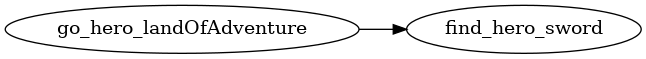
\includegraphics[width=0.7\textwidth]{seq1.png}}
\vspace{7mm}
\end{figure}

The \emph{Then} keyword denotes that the event is the next stage in a sequence
of events. However, this keyword is syntactic sugar, and can be omitted for the same effect:

\begin{lstlisting}[label={lst:seq3}, caption={``The'' instead of ``Then''}]
The Hero goes to the Land of Adventure
The Hero finds the Sword
\end{lstlisting}

Events can be strung together in a sequence that is as long as the author needs:

\begin{lstlisting}[label={lst:seq4}, caption={A sequence of events}]
The Hero goes to the Land of Adventure
Then the Hero finds the Sword
Then the Hero meets the Villain
Then the Hero kills the Villain
Then the Hero returns Home
\end{lstlisting}

\vspace{7mm}
\centerline{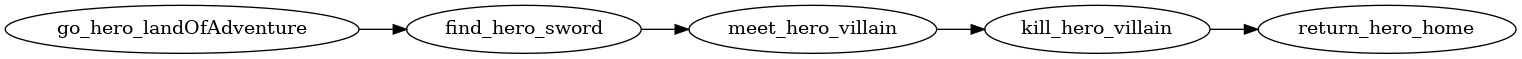
\includegraphics[width=\textwidth]{seq2.png}}
\vspace{7mm}

The author can use any verb they wish to describe an event. The verbs are
stemmed using \emph{WordNet}~\citep{miller1995wordnet} so that, for example,
\emph{goes} becomes \emph{go} and \emph{wanted} becomes \emph{want} when the
tropes are compiled. The reason for this is consistency: it allows an author to
re-use verbs in any form throughout the trope. For example, they can write ``The
Hero goes Home'', ``The Hero went Home'' or ``The Hero may go Home'', and the
compiled code will be the same.

\subsection{Obligations}
\label{sec:obl-code}
All of the code examples up to this point express events that \emph{may} occur
in the story. When compiled to InstAL, and expressed in terms of norms, they
describe the \emph{permitted} behaviour of the agents in a story. This way, the
character agents are aware of the actions available to them that follow the path
of the author's narrative. However, there are other actions that an author may
want to strongly encourage an agent to take, so that they can direct their
actions with more control (as per requirement R\ref{req:direct}). The syntax for this type of action
is expressed with the \emph{must} keyword, and is shown in
listing~\ref{lst:obl1}. In this case, the first action (\emph{The Hero goes
  Home}) is expressed as a permission, but the second action (\emph{Then the
  Hero must go to the Land of Adventure}) is an obligation.

\begin{lstlisting}[label={lst:obl1}, caption={An obliged event within a trope}]
The Hero goes Home
Then the Hero must go to the Land of Adventure
\end{lstlisting}

\subsubsection{Deadline Events and Consequences}
Obligations may have optional deadline events and consequences. The consequence
event is triggered if the obligation has not been fulfilled before the deadline
event has occurred. Listing~\ref{lst:obl2} shows an example trope where the Hero
is obliged to go to the Land of Adventure before the Villain character kills the
Mentor character. If the Villain kills the Mentor and the Hero has not yet gone
to the Land of Adventure, then a possibility opens up for the Villain to kill
the Hero in the story.

\begin{lstlisting}[label={lst:obl2}, caption={An obliged event with a deadline
and a consequence}]
The Hero must go to the Land of Adventure before the Villain kills the Mentor
  Otherwise, the Villain kills the Hero
\end{lstlisting}

This mechanism could be used as a method of creating branches in the story. If the
specified event happens before the deadline event, the path of the trope goes
one way. If it doesn't, the story follows the path of the consequence event.
Section~\ref{sec:instal-obl} explains in detail how obligations, deadlines and
consequences are compiled to InstAL code.

\subsection{Branching Events}
\label{sec:branch-code}
As requirement R\ref{req:branches} states, a trope author may want to describe alternative possibilities in their story,
where either the player or a character in the story may choose from one of
multiple actions to take. This is implemented using the \emph{Or} keyword in
TropICAL, along with a single indentation level of two spaces to indicate its
dependency on the preceding statement:

\begin{lstlisting}[label={lst:branch1}, caption={Two branches}]
The Hero goes to the Land of Adventure
  Or Hero finds the Sword
\end{lstlisting}

\vspace{7mm}
\centerline{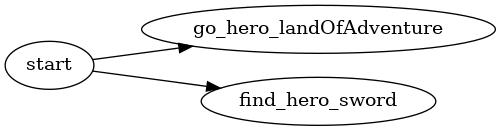
\includegraphics[width=0.5\textwidth]{branch1.png}}
\vspace{7mm}

The above code describes two alternative events: either the Hero can go to the
Land of Adventure, or the Hero can find the Sword.
Multiple events can be chained together on the same level of indentation to create
multiple possible alternatives:

\begin{lstlisting}[label={lst:branch2}, caption={Five branches}]
The Hero goes to the Land of Adventure
  Or the Hero finds the Sword
  Or the Hero meets the Villain
  Or the Hero kills the Villain
  Or the Hero returns Home
\end{lstlisting}

\vspace{7mm}
\centerline{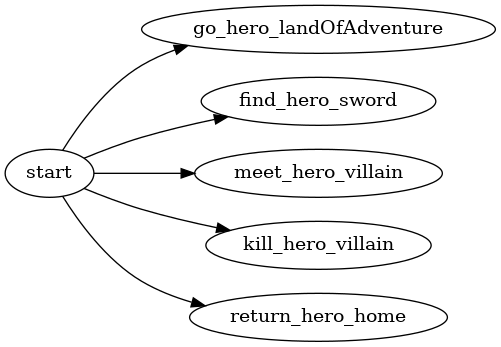
\includegraphics[width=0.5\textwidth]{branch2.png}}
\vspace{7mm}

In the above example, the trope begins with five different possible alternative
events, representing five paths through the story.
These branching events can be combined with the event sequences described
previously to create more complex tropes:

\begin{lstlisting}[label={lst:branch3}, caption={A combination of branches and sequences}]
The Hero goes Home
Then the Hero finds a Sword
  Or the Hero goes to the Land of Adventure
  Or the Hero kills the Villain
Then the Hero meets the Mentor
  Or the Hero goes to the Realm of Mystery
\end{lstlisting}

\vspace{7mm}
\centerline{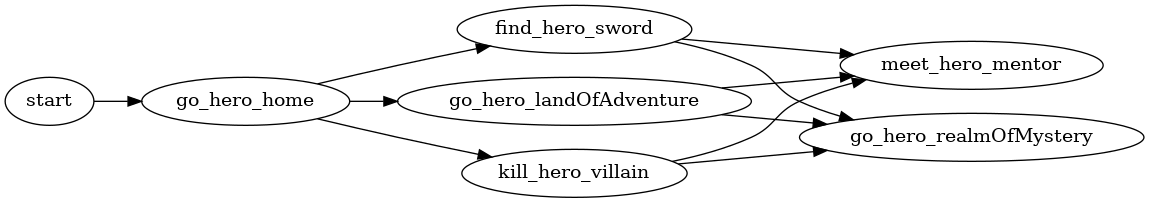
\includegraphics[width=\textwidth]{branch3.png}}
\vspace{7mm}

In the previous example, only one event occurs in each branching story path
before merging back into the main course of the story. In order to extend each
story path further, we use a further level of indentation.

\begin{lstlisting}[label={lst:branch4}, caption={Extending branches}]
The Hero goes Home
Then the Hero finds a Sword
  Or the Hero goes to the Land of Adventure
    Then the Hero finds a Treasure
    Then the Hero drowns
  Or the Hero kills the Villain
    Then the Hero runs Home
      Or the Hero cries
Then the Hero meets the Mentor
  Or the Hero goes to the Realm of Mystery
    Then the Hero meets the Wizard
    Then the Wizard casts a Spell
\end{lstlisting}

\vspace{7mm}
\centerline{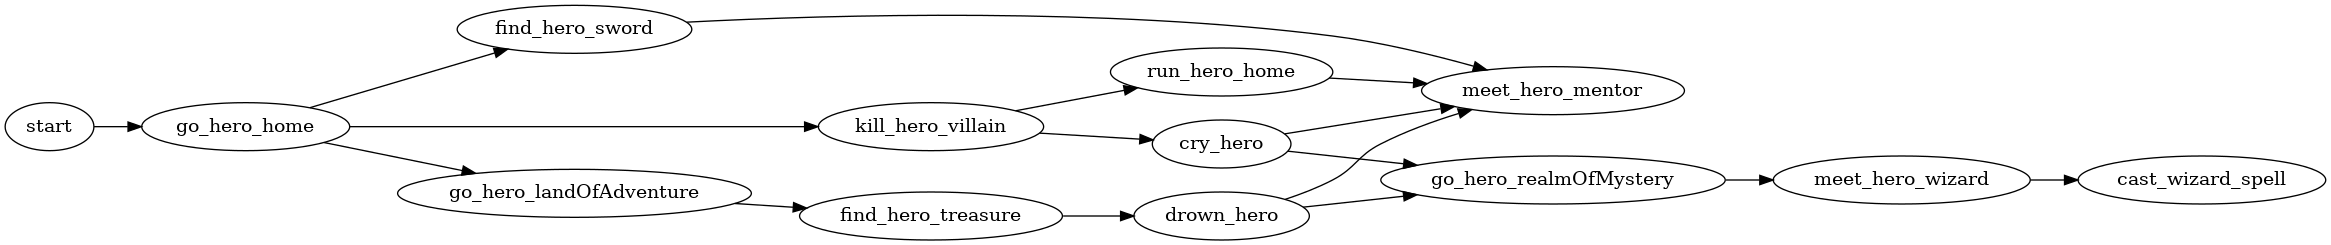
\includegraphics[width=\textwidth]{branch4.png}}
\vspace{7mm}

It should be noted that all branches will merge back into the ``main'' story
path (the bottom level of indentation) once they have completed. To prevent this
from happening, and terminate the story, the author may write \emph{``Then the
  Story ends''}. In this example, the story will always end unless the Hero goes
to the Way Out or escapes the Dark Room:

\begin{lstlisting}[label={lst:branch5}, caption={Terminating branches}]
The Hero goes to the House
Then the Hero meets the Villain
Then the Hero kills the Villain
  Or the Villain kills the Hero
    Then the Story ends
Then the Hero goes to the Way Out
  Or the Hero goes to the Dark Pit
    Then the Crocodile eats the Hero
    Then the Story ends
  Or the Hero goes to the Dark Room
    Then the Hero escapes
      Or the Grue eats the Hero
        Then the Story ends
Then the Hero finds the Treasure
\end{lstlisting}

\vspace{7mm}
\centerline{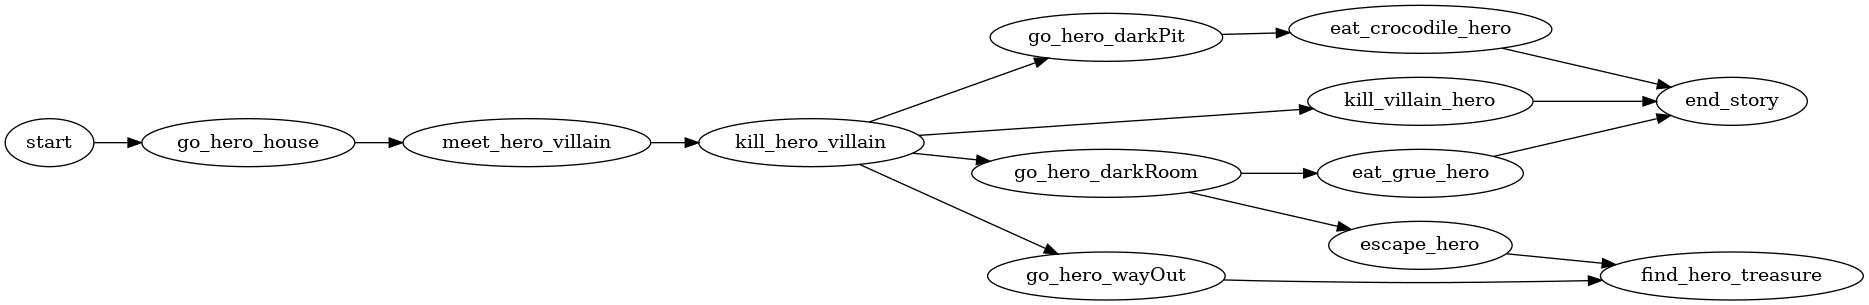
\includegraphics[width=\textwidth]{branch5.png}}
\vspace{7mm}

Using this technique, branches can be extended indefinitely through increasing
levels of indentation.
Deeply indented tropes are often undesirable, however, and is usually a symptom
that a trope needs to be subdivided. We can achieve this by
embedding subtropes inside of other tropes.

\subsection{Subtropes}
\label{sec:subtrope-code}
Requirement R\ref{req:subtropes} states that we need a mechanism for the
nesting of tropes, so that we may create new abstractions by combining existing
tropes to create new ones. We do this through \emph{Subtropes}, which are simply previously-written tropes that are embedded inside a
new trope. Take this simple trope example:

\begin{lstlisting}[showstringspaces=false, label={lst:subtrope1}, caption={Subtrope
to be embedded}]
"Item Search" is a trope where:
   The Macguffin is an object
   The Hero is a role
   Home is a place

   The Hero chases the Macguffin
   Then the Hero finds the Macguffin
     Or the Hero goes Home
\end{lstlisting}

\vspace{7mm}
\centerline{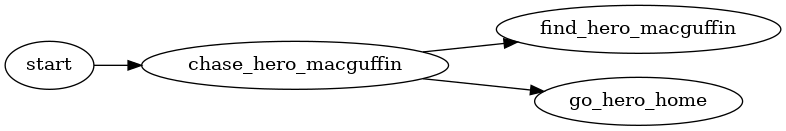
\includegraphics[width=0.7\textwidth]{subtrope1.png}}
\vspace{7mm}

To embed this trope inside another trope, we refer to it by name by writing
\emph{Then the ``Item Search'' trope happens}. It is important to put the name
of the trope inside quotation marks. The reason for this is that it makes
subtrope embedding statements easier to parse, as trope names may contain
combinations of role, object and place names along with verbs. Putting the name
of a trope inside quotation marks ensures that the parser will not confuse it
with any other kind of statement. An example of putting this trope at the end
of another trope is shown in the following example:

\begin{lstlisting}[showstringspaces=false, label={lst:subtrope2}, caption={Trope containing a subtrope}]
"Kill then Search" is a trope where:
  Away is a place
  The Hero is a role
  The Villain is a role

  The Hero goes Away
  Then the Hero kills the Villain
  Then the "Item Search" trope happens
\end{lstlisting}

\vspace{7mm}
\centerline{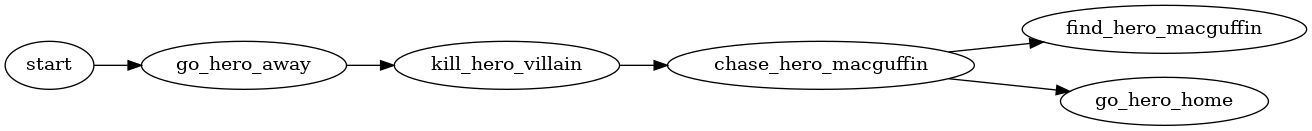
\includegraphics[width=\textwidth]{subtrope2.png}}
\vspace{7mm}

The ``Item Search'' subtrope is thus embedded inside the ``Kill then Search''
trope, with all of the events and branches of ``Item Search'' being appended to
the end of ``Kill then Search''. Rather than only being embedded at the end of a
trope however, subtropes can appear at any point in a trope, or even at several
points in a trope. Take this example that uses the ``Item Search'' trope inside
nested branches of its story:

\begin{lstlisting}[showstringspaces=false, label={lst:subtrope3}, caption={Subtrope in multiple places}]
"Futile Search" is a trope where:
  The Hero is a role
  The Villain is a role
  The Mentor is a role
  Away is a place
  Home is a place
  The Land of Adventure is a place
  The Realm of Mystery is a place

  The Hero goes Away
  Then the Hero meets the Villain
    Or the Hero meets the Mentor
      Then the "Item Search" trope happens
  Then the Hero kills the Villain
  Then the "Item Search" trope happens
\end{lstlisting}

\vspace{7mm}
\centerline{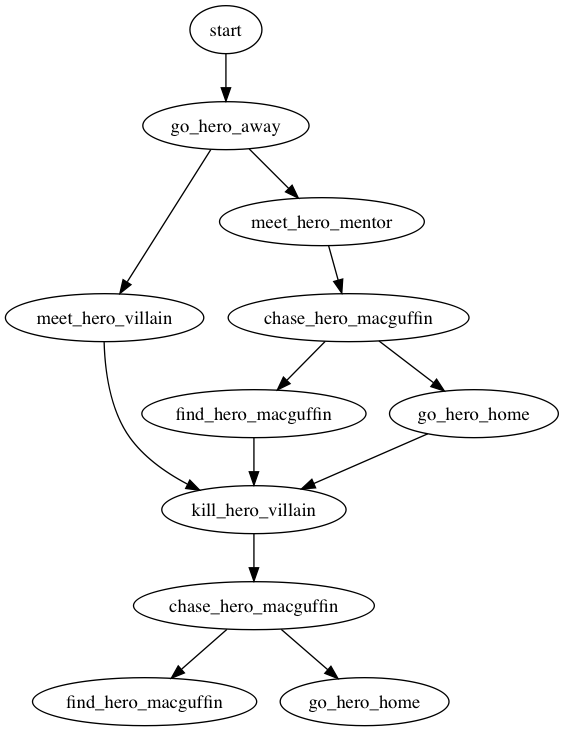
\includegraphics[width=0.5\textwidth]{subtrope3.png}}
\vspace{7mm}

An author can create complex branching narrative by combining these tropes together. To see
visualisations of the story paths of multiple tropes combined, see
section~\ref{sec:combining-tropes} of Chapter~\ref{cha:storybuilder}.

For technical details of the parser implementation, including the EBNF grammar
of the TropICAL language, refer to Appendix~\ref{appendix:t-grammar}.
% Appendix~\ref{appendix:parse-tree} shows visualisations of the parse tree output for some
% of the code examples described in this section.

\section{InstAL Code Generation}
\label{sec:t-codegen}
% TODO intro: 1
% TODO tech discussion: 1
This section describes how and why language features translate to
InstAL, with fully translated examples of InstAL code appearing in Appendix~\ref{appendix:instal}.

\subsection{Answer Set Programming (ASP)}
\added{
Answer Set Programming (ASP) uses a \emph{declarative} programming paradigm, meaning
that programs described in an ASP language (such as AnsProlog) describe the
problem itself, whereas traditional programming languages (such as Java or
Python) describe the solution to the problem. For example, a \emph{Sudoku} game
would be created by logically describing the rules of the game, which are used
to search for potential solutions when given number grids as input. Contrast
this with the traditional programming approach, which would be to describe the
steps that are taken when a Sudoku game is played.

An ASP program consists of three elements: a knowledge base of ``facts'', rules
for generating new facts, and constraints that limit the number of new facts
that can be generated. In the example of a Sudoku solver, the program itself
would consist of the game rules (that numbers 1-9 are arranged in 3-by-3 grids),
along with the constraints of the game:

\begin{itemize}
\item No number can be repeated inside a grid
\item No number can be in the same column or row
\end{itemize}

The ``knowledge base'' describes the initial conditions of a Sudoku game: the
numbers that are filled in already. The job of the \emph{Answer Set Solver} is
to generate new facts based on the game rules, but limited by the described
constraints. In this way, it can find the set of possible solutions for any
given game of Sudoku.

Finding solutions for an ASP program is a two-step process. The first step is to
\emph{ground} any free variables in the program rules. This is done by
generating facts to replace all the possible values of each variable. The Answer
Set Solver then searches the space of
these possible solutions to find those that are \emph{stable} (ones that do not
contain any contradictions).

The benefit of using ASP over Prolog comes from its use of the \emph{stable
  model semantics}, which allows for the use of \emph{negation as failure}
without the risk of an ASP program getting stuck in an infinite loop. As each
free variable is \emph{grounded} (the space of all possible values for a
variable is generated), a search for solutions should terminate even when
negation is used.
}{2.4.2: Brief introduction to ASP}

\subsection{InstAL: The Institution Action Language}
\label{sec:instal-intro}
\added{
}{2.4.2: Introduction to InstAL}
Cliffe's thesis~\citep{cliffe2007specifying} introduces \emph{InstAL}, a
programming language for the specification of Social Institutions (such as those
described in Section~\ref{sec:lit-insts}) for multi-agent systems. InstAL code
compiles to the AnsProlog language for Answer Set Programming, allowing the use
of an answer set solver to generate answer sets corresponding to permitted and
obliged agent actions. This section provides a brief introduction to the InstAL
institutional model.

\subsubsection{Fluents}
These are properties that may or may not hold true at some instant in time, and that change over the course of time. \emph{Institutional events} are able to \emph{initiate} or \emph{terminate} fluents at points in time. A fluent could describe whether a character is currently on stage, the scene of the story that is currently being acted out, or whether or not the character is happy at that moment in time.
Domain fluents ($\mathcal{D}$) describe domain-specific properties that can hold at a certain point in time. 

Institutional fluents consist of (institutional) \emph{powers}, \emph{permissions} and \emph{obligations}.
% check your facts on this one
An \textbf{institutional power} ($\mathcal{W}$) describes whether or not an external event has the authority to generate a meaningful institutional event. Taking an example from Propp's formalism, an \emph{absentation\/} event can only be generated by an external event brought about by a \emph{donor\/} character (such as their leaving the stage). Therefore, any characters other than the donor character would not have the institutional power to generate an \emph{absentation\/} institutional event when they leave the stage.

\subsubsection{Permissions} ($\mathcal{P}$) are associated with external actions that agents are permitted to do at a certain instant in time. These can be thought of as the set of \emph{socially permitted\/} actions available to an agent. While it is possible for an agent to perform other actions, societal norms usually discourage them from doing so.
% PJ examples
% For example, it would not make sense in the world of Punch and Judy if Punch were to give the sausages to the Policeman. It is always Joey who gives the sausages to Punch. Also, it would be strange if Joey were to do this in the middle of a scene where Punch and Judy are arguing. We make sure agents'' actions are governed so as to allow them only a certain subset of permitted actions at any one time.

\subsubsection{Obligations} ($\mathcal{O}$) are institutional facts that contain actions agents \emph{should} do before a certain deadline. If the action is not performed in time, a \emph{violation event} is triggered, which may result in a penalty being incurred. While an agent may be obliged to perform an action, it is entirely their choice whether or not they actually do so. They must weigh up whether or not pursuing other courses of action is worth accepting the penalty that an unfulfilled obligation brings.

\subsubsection{Events}
\label{sec:inst-events}
% actually 3 kinds, including violation events
Cliffe's model specifies three types of \textbf{event}: \emph{external events} (or `observed events', $\mathcal{E}_{obs}$), \emph{institutional events} ($\mathcal{E}_{instevent}$) and \emph{violation events} ($\mathcal{E}_{viol}$). Examples of each are given in Figure~\ref{fig:events-pj}.
\emph{External events} are observed to happen in the agents' environment, which can \emph{generate} \emph{institutional events} which occur only within the institional model, leading to the \emph{initiation} or \emph{termination} of (domain) fluents, permissions, obligations or institutional powers.
An external event could be an agent leaving the stage, an agent hitting another,
or an agent dying. Internal events include narrative events such as scene
changes, or the triggering of story functions such as Propp's \emph{absentation} or \emph{interdiction} (described in Section~\ref{sec:formalisms}). 

Violation events occur when an agent has failed to fulfil an obligation before the specified deadline. These can be implemented in the form of a penalty, by decreasing an agent's health, for example.

\subsubsection{Event Generation and Consequences}
An \textbf{event generation} function, $\mathcal{G}$, describes how events
($\mathcal{E}$, usually external, but can also be internal) %
can generate other (usually institutional) events, conditional upon the current institutional state ($\cal X$). This is the counts-as relation.

Event generation functions follow a $\langle \mathtt{preconditions} \rangle \rightarrow \{\mathtt{postconditions}\}$ format. The preconditions consist of a set of fluents that hold at that time, along with an event to have occurred. The postconditions are the events that are generated. The generation functions are used to generate internal, institutional events from external events.

\textbf{Consequences} consist of fluents, permissions and obligations that are \emph{initiated} ($\mathcal{C}^{\uparrow}$) or \emph{terminated} ($\mathcal{C}^{\downarrow}$) by institutional events. 

A full example of an institution for the ``Punch and Judy'' story world,
described in terms of story tropes, appears in Section~\ref{sec:tropes-as-insts}.

\subsection{Why use ASP and InstAL?}
\label{sec:why-asp-instal}
\added{
Answer Set Programming is a useful tool for describing tropes and stories, as it
allows us to formally construct a story model, against which possible sequences
of events can be checked to see if they are allowed within that model.

As we are simulating our story world with a Multi-Agent System, we need to be
able to determine which agent actions are allowed within the story model, given
a history of past events that have already occurred. Using an answer set solver,
we can query the model to check which agent actions are valid (according to the
story) while the simulation is running.

Additionally, when designing our story model, the use of an answer set solver
allows us to generate answer sets corresponding to all of the possible paths
through a story. This can be useful when attempting to visualise the branches
that are created when decision points are inserted into the TropICAL trope
descriptions. The StoryBuilder tool described in Chapter~\ref{cha:storybuilder}
makes use of this feature of ASP to generate tree diagrams to visualise the
possible paths through a story during the process of creating tropes with TropICAL.

The advantage of using ASP over similar alternatives such as Prolog is its
handling of negation-as-failure. Due to its use of the stable model semantics,
queries to an answer set solver are less likely to get stuck in infinite loops.
This makes ASP suitable for use at run time in situations such as a multi-agent
system story model simulation.

Our TropICAL language compiles to InstAL before being compiled to the AnsProlog
implementation of ASP. This offers several benefits. The first is that it
greatly simplifies the process of code generation---rather than having to write
a compiler to generate AnsProlog code, it can instead generate a smaller
quantity of InstAL code, which can then generate the AnsProlog.

There are other benefits besides convenience, however. InstAL provides a
ready-made formal model that describes event-driven scenarios in terms of social
norms. As long as our tropes are described in terms of events that occur in a
story, they can be translated into this formal model. This allows great
flexibility in the definition of tropes, so that authors can describe them
semi-informally in a language that resembles natural English. Once events of a
trope are described this way, it is relatively straightforward to describe them
in terms of permissions and obligations in InstAL.

Another benefit of using InstAL is that its institutional model allows us to
observe when characters deviate from the story path, by generating violation
evens. When a violation event occurs, the potentially story-breaking action can
be handled using a strategy such as changing the active tropes in the running
simulation (Section~\ref{sec:freedom-example} gives an example of how this kind
of scenario can be dealt with).
}{2.4.2: Explanation of why ASP and InstAL were chosen}

\subsection{Compilation Strategy}

The steps that the TropICAL compiler goes through to produce InstAL code are the
following:

\begin{enumerate}
\item \textbf{Parse entity definitions}: The parser only looks at the first
  lines of the file that define the roles, objects and places (such as \emph{The
    Hero is a role} or \emph{The Sword is an object})
\item \textbf{Parse the trope's events}: The parser then examines the rest of
  the trope, with the previously defined entity definitions inserted into the
  parser's grammar as keywords.
\item \textbf{Transform the parse tree into a hash map}: The hash map is an
  intermediate representation of the trope entities and events described in the
  TropICAL code.
\item \textbf{Generate InstAL institutions from the hash map representation}:
  The hash map representation of each TropICAL trope is converted into a corresponding InstAL institution.
\end{enumerate}

Once the tropes written in TropICAL have been parsed and converted into an
intermediate hash map, this data structure is then used to generate InstAL code.
Each TropICAL trope compiles to a separate InstAL institution, each of which is
contained in its own file. Example pieces of code of the anatomy of an InstAL institution are
shown in Listing~\ref{lst:instal-anatomy}. 

An InstAL institution contains the following parts:

\begin{itemize}
\item \emph{Institution Name}: the name of the insitution
  (line~\ref{lne:inst-name} of Listing~\ref{lst:instal-anatomy})
\item \emph{Type Declarations}: types of entity that appear in the institution,
  such as Agent, Object, and Place (lines~\ref{lne:type-start} -~\ref{lne:type-end})
\item \emph{Fluent Declarations}: fluents are facts that tell us something about
  the agents' environment (lines~\ref{lne:fluent-start} -~\ref{lne:fluent-end})
\item \emph{Exogenous Event Declarations}: exogenous (external) events are
  events that occur in the agents' environment, such as actions taken by the
  agents, as opposed to actions that occur within an institution
  (lines~\ref{lne:ex-start} -~\ref{lne:ex-end})
\item \emph{Violation Event Declarations}: events that are triggered when obligations
  are not fulfilled (line~\ref{lne:viol-event})
\item \emph{Institutional Event Declarations}: these are events that occur
  inside the institution to initiate and terminate norms (permissions and
  obligations) and fluents. They are generated by the exogenous events, and have
  a name that is prefixed with ``int'' (such as ``intHerosJourney'')
  (lines~\ref{lne:instev-start} -~\ref{lne:instev-end})
\item \emph{Obligation Fluent Declarations}: obligation fluents have three
  parts: the institutional event that is obliged to happen, the institutional
  event that acts as a deadline, and the violation event. The institutional
  (obligation) event must occur before the deadline event happens. If the deadline event
  happens before the obligation event, then the violation event is triggered
  (line~\ref{lne:obl-fluent}, obligation events are described further in Section~\ref{sec:instal-obl})
\item \emph{Norm / fluent initiation events}: this part of an institution
  specifies which norms and fluents are initiated by its institutional
  (internal) events (lines~\ref{lne:init-start} -~\ref{lne:init-end}, described
  in Section~\ref{sec:anat-init})
\item \emph{Norm / fluent termination events}: this specifies which norms and
  fluents are terminated by institutional events (lines~\ref{lne:term-start}
  -~\ref{lne:term-end}, described in Section~\ref{sec:termination})
\item \emph{Generation events}: institutional events that are generated by
  exogenous (external) events (line~\ref{lne:gen-start} -~\ref{lne:gen-end},
  described in Section~\ref{sec:anat-gen})
\item \emph{Norms / fluents that hold initially in the institution}: this
  describes the initial state of the institution when it becomes active,
  consisting of the norms corresponding to the trope's first event, and the
  fluents that describe the role, object and place entities in the trope
  (lines~\ref{lne:initially-start} -~\ref{lne:initially-end}, described in Section~\ref{sec:anat-initial})
\end{itemize}

\subsubsection{Intermediate Hash Map Representation}
\added{}{2.4.1: Added a new section to explain the hash map that TropICAL code compiles
  to}

Once a TropICAL definition of a trope has been parsed, its parse tree is
converted into a hash map, which is used as an intermediate data structure from
which different outputs can be produced. A hash map consists of key-value pairs,
and is used as a table to look up values that correspond to certain keys.

In our case, we are generating the
InstAL code from this hash map, but the purpose of using this intermediate data
structure is to simplify the process of compiling to other programming
languages. This would make it easier, for example, to add code that generates
AnsProlog code directly rather than compiling to InstAL first.

The format of the hash map is as follows:

\begin{itemize}
  \item \textbf{Label}: A string representing the name of the trope
  \item \textbf{Events}: A list of events that occur in the trope (see below for
    a description of an event)
  \item \textbf{Roles}: A list of strings describing character names for the trope
  \item \textbf{Objects}: A list of strings that are names of objects in the trope
  \item \textbf{Locations}: A list of strings naming places in the trope
\end{itemize}

Each event is a separate hash map consisting of a subject (which corresponds to a \emph{role} key), a
predicate (a \emph{verb} key) and an object. The object key can be a
\emph{role}, \emph{object} or \emph{place}. In the case where both subject and object are roles, the keys are renamed
to \emph{role-a} and \emph{role-b}.
In the case where branching events occur in a trope, the event's only key is
\emph{or}, whose value is a list of alternative events that could happen.

Listing~\ref{lst:macguffin-listing} shows a simplified ``MacGuffin'' trope in
TropICAL. Once this trope has been parsed, its parse tree is processed and
converted to the hash map representation shown in
Listing~\ref{lst:macguffin-hashmap}. In the listing, a hash map is contained
inside curly braces, with keys being unquoted words preceded by a colon and
values immediately following keys. Lists of values
are contained inside square brackets.

\begin{lstlisting}[showstringspaces=false, label={lst:macguffin-listing},
caption={A simplified example of the ``MacGuffin'' trope}]
"MacGuffin" is a trope where:
  The Macguffin is an object
  The Hero is a role
  The Villain is a role
  Home is a place
  The Hero chases the Macguffin
  Then the Hero finds the Macguffin
    Or the Villain finds the Macguffin
  Then the Hero goes Home
\end{lstlisting}

\begin{lstlisting}[showstringspaces=false, label={lst:macguffin-hashmap},
caption={Hash Map representation of the ``MacGuffin trope from Listing~\ref{lst:macguffin}''}]
{:label "MacGuffin",
 :events [{:role "Hero", :verb "chase", :object "Macguffin"},
          {:or [{:role "Hero", :verb "find", :object "Macguffin"}
                {:role "Villain", :verb "find", :object "Macguffin"}]}
          {:role "Hero", :verb "go", :place "Home"}],
 :roles ("The Hero" "The Villain"),
 :objects ("The Macguffin"),
 :locations ("Home")}
\end{lstlisting}

When a trope's hash map representation is converted into InstAL, each entity
(role, place, object) is assigned a letter to be used as a variable in the
InstAL events. For example, the \emph{intHerosJourney} institutional event on
line~\ref{lne:instev-start} of Listing~\ref{lst:instal-anatomy} is declared with four parameters of types
\emph{Agent, Agent, PlaceName, PlaceName}. When this institutional event is used
to initiate fluents on line~\ref{lne:init-start}, its parameters are input as
variables \emph{R, S, T} and \emph{U}. In the original trope definition, the
\emph{Hero's Journey} contains the \emph{Hero}, \emph{Villain} and \emph{Mentor}
roles, and the \emph{Land of Adventure} location. When the
\emph{intHerosJourney} event happens, its variables are filtered using the
\emph{if} keyword to ensure that $R = \textit{Hero}$, $S = \textit{Villain}$, $T
= \textit{Mentor}$ and $U = \textit{Land of Adventure}$. An example of this
appears on lines~\ref{lne:init-vars} and~\ref{lne:init-end} of Listing~\ref{lst:instal-anatomy}.

\begin{figure}[!h]
\begin{minipage}{0.8\textwidth}
\begin{lstlisting}[caption={Anatomy of an InstAL institution},basicstyle=\scriptsize\ttfamily,label=lst:instal-anatomy,escapechar=\~]
institution herosJourney;~\label{lne:inst-name}~

% TYPES ----------
type Agent;~\label{lne:type-start}~
type Role;
type Phase;~\mylabel{t0}\label{lne:type-end}~

% FLUENTS ----------
fluent role(Agent, Role);~\label{lne:fluent-start}~
fluent phase(Trope, Phase);~\mylabel{t1}\label{lne:fluent-end}~

% EXTERNAL EVENTS ----------
exogenous event kill(Agent, Agent);~\label{lne:ex-start}~
exogenous event go(Agent, PlaceName);~\mylabel{t2}\label{lne:ex-end}~

% VIOLATION EVENTS ----------
violation event violHeroGoLandOfAdventure;~\mylabel{t3}\label{lne:viol-event}~

% INST EVENTS ----------
inst event intHerosJourney(Agent, Agent, PlaceName, PlaceName);~\label{lne:instev-start}~
inst event intKill(Agent, Agent);
inst event intGo(Agent, PlaceName);~\mylabel{t4}\label{lne:instev-end}~

% OBLIGATION FLUENTS ----------
obligation fluent obl(intGo(Agent, PlaceName), intKill(Agent, Agent), violHeroGoLandOfAdventure);~\mylabel{t5}\label{lne:obl-fluent}~

% INITIATES ----------
intHerosJourney(R, S, T, U) initiates~\label{lne:init-start}~
    phase(herosJourney, phaseA),
    perm(go(R, U)) if
        phase(herosJourney, active),
        role(R, hero),~\label{lne:init-vars}~
        place(U, landOfAdventure);~\mylabel{t6}\label{lne:init-end}~

% TERMINATES ----------
intHerosJourney(R, S, T, U) terminates~\label{lne:term-start}~
    phase(herosJourney, phaseA),
    perm(go(R, U)) if
        phase(herosJourney, phaseA),
        role(R, hero),
        place(U, landOfAdventure);~\mylabel{t7}\label{lne:term-end}~

% GENERATES ----------
go(R, U) generates~\label{lne:gen-start}~
    intHerosJourney(R, S, T, U) if
        role(R, hero),
        place(U, landOfAdventure);
kill(S, T) generates
    intHerosJourney(R, S, T, U) if
        role(T, mentor),
        role(S, villain);~\mylabel{t8}\label{lne:gen-end}~

% INITIALLY -----------
initially~\label{lne:initially-start}~
    pow(intHerosJourney(R, S, T, U)) if role(R, hero), role(S, villain), role(T, mentor), place(U, landOfAdventure);
    perm(intHerosJourney(R, S, T, U)) if role(R, hero), role(S, villain), role(T, mentor), place(U, landOfAdventure);
    perm(kill(S, T)) if role(T, mentor), role(S, villain);
    phase(herosJourney, active),
    role(lukeSkywalker, hero),~\label{lne:roledef-start}~
    role(darthVader, villain),
    role(obiWan, mentor),
    place(japan, landOfAdventure);~\mylabel{t9}\label{lne:initially-end}~

\end{lstlisting}
\end{minipage}\hspace{0.08\textwidth}%\hfill
\begin{minipage}{0.12\textwidth}\scriptsize
  \myref{t0}{s0}{Type declarations}
  \myref{t1}{s1}{Fluent declarations}
  \myref{t2}{s2}{Exogenous event declarations}
  \myref{t3}{s3}{Violation event declarations}
  \myref{t4}{s4}{Institutional event declarations}
  \myref{t5}{s5}{Obligation fluent declarations}
  \myref{t6}{s6}{Norm / fluent initiation events}
  \myref{t7}{s7}{Norm / fluent termination events}
  \myref{t8}{s8}{Generation events}
  \myref{t9}{s9}{Norms / fluents that hold initially in the institution}
\end{minipage}
\end{figure}

The following sections describe how each part of a TropICAL trope compiles to
the components of an InstAL institution as show above and in Listing~\ref{lst:instal-anatomy}.

\subsection{Initial Conditions}
% TODO before / after snippets: 2
% TODO explanation: 2
% TODO explain how the domain works in InstAL
\label{sec:anat-initial}
The \emph{initially} clause in InstAL specifies the fluents that initially hold
when the institution is effected. Role, object and place declarations are
translated into fluent declarations as part of this clause. For example, for a
trope with the following declarations:

\begin{lstlisting}
The Hero is a role
The Sword is an object
The Land of Adventure is a place
\end{lstlisting}

And the following entity instances:

\begin{lstlisting}
Luke Skywalker is a Hero
The Lightsaber is a Sword
The Death Star is a Land of Adventure
\end{lstlisting}

The following InstAL code is produced, with type and fluent declarations
automatically appearing at the top of the file:

\begin{lstlisting}
type Agent;
type Role;
type Place;
type PlaceName;
type Object;
type ObjectName;

fluent role(Agent, Role);
fluent place(PlaceName, Place);
fluent object(ObjectName, Object);

initially:
  role(lukeSkywalker, hero),
  object(lightSaber, sword),
  place(deathStar, landOfAdventure);
\end{lstlisting}

The \emph{initially} clause also specifies the permitted and obliged events that
occur at the start of the trope. Say our trope contains a series of events (as in
listing~\ref{lst:seq4}):

\begin{lstlisting}
The Hero goes to the Land of Adventure
Then the Hero finds the Sword
Then the Hero meets the Villain
Then the Hero kills the Villain
Then the Hero returns Home
\end{lstlisting}

In this case, the first event of the trope (\emph{The Hero goes to the Land of
  Adventure}) must be permitted to happen at the very beginning of the
institution, inside the \emph{initially} clause. In combination with the above
entity declarations, this results in the following code being generated
(omitting the type and fluent declarations this time):

\begin{lstlisting}
initially:
  perm(go(X, Y)) if role(X, hero), place(Y, landOfAdventure),
  role(lukeSkywalker, hero),
  object(lightSaber, sword),
  place(deathStar, landOfAdventure);
\end{lstlisting}

This means that the Luke Skywalker character is able to go to the Death Star at the beginning
of the institution, as is specified in the trope.

\subsection{Generation}
% TODO before / after snippets: 2
% TODO explanation: 2
\label{sec:anat-gen}

Tropes usually consist of multiple events, so it is not enough to have one event
permitted at the start of a trope. Once this first event has occurred, the next
event in the sequence must have permission to happen.

As described previously in Section~\ref{sec:inst-events}, an institution
consists of three types of events: \emph{external events} (events that occur in
the agents' environment), \emph{intstitutional
  events} (events triggered inside an institution) and \emph{violation events}
(events that occur when an obligation is violated in an institution). The institution watches for events to happen as \emph{external} events in the
environment, and then has these events generate \emph{institutional} events that
occur within the institution and create permissions or obligations for further
external events to occur. Returning to Listing~\ref{lst:seq4} above, the
external events that happen are:

\begin{itemize}
  \item The Hero finds the Sword
  \item The Hero meets the Villain
  \item The Hero kills the Villain
  \item The Hero returns Home
\end{itemize}

These are translated into \emph{generates} statements in InstAL so that they
generate the required institutional events (denoted with an ``int''
prefix, following the naming convention introduced in
Section~\ref{sec:inst-events}):

\begin{lstlisting}[showstringspaces=false, label={lst:instal-generates},
caption={InstAL code resulting from the compilation of Listing~\ref{lst:seq4}}]
find(R, T) generates
    intSequence3(R, S, T, U, V) if
        role(R, hero),
        object(T, sword);
kill(R, S) generates
    intSequence3(R, S, T, U, V) if
        role(S, villain),
        role(R, hero);
meet(R, S) generates
    intSequence3(R, S, T, U, V) if
        role(S, villain),
        role(R, hero);
go(R, V) generates
    intSequence3(R, S, T, U, V) if
        role(R, hero),
        place(V, landOfAdventure);
return(R, U) generates
    intSequence3(R, S, T, U, V) if
        role(R, hero),
        place(U, home);
\end{lstlisting}

Each institution only has one institutional event that is triggered by the
external events, which is named after the trope itself (in this case, the event
is named \emph{intSequence3} after the trope name ``Sequence 3''). The
permissions and obligations that this institutional event initiates depend on
the \emph{phase} of the trope that is currently active (see
section~\ref{sec:event-phases}) below.

\subsection{Initiation}
% TODO before / after snippets: 2
% TODO explanation: 2
\label{sec:anat-init}

External events generate an internal event for the institution, which permits
the next event or events in a sequence to occur. To ensure that the events of
the trope are permitted or obliged to occur one after another, we use a
mechanism called \emph{event phases}.

\subsubsection{Event Phases}
\label{sec:event-phases}
An \emph{event phase} is a fluent that holds the state of the current
institution (described previously in Section~\ref{sec:trope-phases}). At the beginning of the trope, its state is simply \emph{active}.
This is represented in the institution through the fluent \emph{phase(tropeName,
active)}.
Once the first event has occurred, the trope enters \emph{phase A}, which means
that the fluent \emph{phase(tropeName, phaseA)} then holds, and the
\emph{phase(tropeName, active} fluent is terminated (this is described in
section~\ref{sec:termination}). This initiation and termination process then
repeats through all phases of the trope, through phases B, C and D if they
exist, until the final event occurs and the last phase is terminated.

In the case of our example sequence of events from Listing~\ref{lst:seq4}, there
are five phases in total:

\begin{itemize}
  \item The Hero goes to the Land of Adventure (active)
  \item The Hero finds the Sword (phase A)
  \item The Hero meets the Villain (phase B)
  \item The Hero kills the Villain (phase C)
  \item The Hero returns Home (phase D)
\end{itemize}

The events and phases of this trope are initiated in InstAL through the
following generated code:

\begin{lstlisting}[label={lst:initiates}, caption={Institutional event
initiation code for Listing~\ref{lst:seq4}}]
intSequence3(R, S, T, U, V) initiates
    phase(sequence3, phaseA),
    perm(find(R, T)) if
        phase(sequence3, active),
        role(R, hero),
        object(T, sword);
intSequence3(R, S, T, U, V) initiates
    phase(sequence3, phaseB),
    perm(meet(R, S)) if
        phase(sequence3, phaseA),
        role(S, villain),
        role(R, hero);
intSequence3(R, S, T, U, V) initiates
    phase(sequence3, phaseC),
    perm(kill(R, S)) if
        phase(sequence3, phaseB),
        role(S, villain),
        role(R, hero);
intSequence3(R, S, T, U, V) initiates
    phase(sequence3, phaseD),
    perm(return(R, U)) if
        phase(sequence3, phaseC),
        role(R, hero),
        place(U, home);
\end{lstlisting}


\subsection{Termination}
\label{sec:termination}
% TODO before / after snippets: 2
% TODO explanation: 2

The generated code that terminates the phases and permissions corresponding to
those initiated in Listing~\ref{lst:initiates} is shown in
listing~\ref{lst:terminates} below. Once an external event occurs, its
permission to occur again is terminated along with the phase in which it occurred:

\begin{lstlisting}[label={lst:terminates}, caption={Institutional event
termination code for Listing~\ref{lst:seq4}}]
intSequence3(R, S, T, U, V) terminates
    phase(sequence3, active),
    perm(go(R, V)) if
        phase(sequence3, active),
        role(R, hero),
        place(V, landOfAdventure);
intSequence3(R, S, T, U, V) terminates
    phase(sequence3, phaseA),
    perm(find(R, T)) if
        phase(sequence3, phaseA),
        role(R, hero),
        object(T, sword);
intSequence3(R, S, T, U, V) terminates
    phase(sequence3, phaseB),
    perm(meet(R, S)) if
        phase(sequence3, phaseB),
        role(S, villain),
        role(R, hero);
intSequence3(R, S, T, U, V) terminates
    phase(sequence3, phaseC),
    perm(kill(R, S)) if
        phase(sequence3, phaseC),
        role(S, villain),
        role(R, hero);
intSequence3(R, S, T, U, V) terminates
    phase(sequence3, phaseD),
    perm(return(R, U)) if
        phase(sequence3, phaseD),
        role(R, hero),
        place(U, home);
\end{lstlisting}

\subsection{Branches}
% TODO before / after snippets: 2
% TODO explanation: 2

To represent branching events in InstAL, multiple events are permitted to occur
during one phase. Take as an example the combination of event sequences and
branches shown in Listing~\ref{lst:branch3}:

\begin{lstlisting}
The Hero goes Home
Then the Hero finds a Sword
  Or the Hero goes to the Land of Adventure
  Or the Hero kills the Villain
Then the Hero meets the Mentor
  Or the Hero goes to the Realm of Mystery
\end{lstlisting}

A fully compiled institution appears in Section~\ref{appendix:branch3} of
Appendix~\ref{appendix:instal}, which uses the following entity instances:

\begin{lstlisting}
Harry Potter is a Hero
Voldemort is a Villain
Dumbledore is a Mentor
The Gryffindor Sword is a Sword
Hogwarts is a Land of Adventure
The Chamber of Secrets is a Realm of Mystery
\end{lstlisting}

The branching events are implemented in the \emph{initiates} and
\emph{terminates} clauses. In Listing~\ref{lst:branch-init} below, we see that three possible events are given
permission to occur as part of Phase A: \emph{The Hero finds a Sword}, \emph{The
  Hero goes to the Land of Adventure}, and \emph{The Hero kills the Villain}. In
Phase B, two events corresponding to the possible branches are given permission
to occur: \emph{The Hero meets the Mentor} and \emph{The Hero goes to the Realm
  of Mystery}:

\begin{lstlisting}[label={lst:branch-init}, caption={Initiation events for the
branching trope in Listing~\ref{lst:branch3}}]
intBranch3(R, S, T, U, V, W, X) initiates
    phase(branch3, phaseA),
    perm(find(R, U)),
    perm(go(R, X)),
    perm(kill(R, S)) if
        phase(branch3, active),
        object(U, sword),
        role(R, hero),
        place(X, landOfAdventure),
        role(S, villain);
intBranch3(R, S, T, U, V, W, X) initiates
    phase(branch3, phaseB),
    perm(meet(R, T)),
    perm(go(R, V)) if
        phase(branch3, phaseA),
        place(V, realmOfMystery),
        role(R, hero),
        role(T, mentor);
\end{lstlisting}

This means that during Phase A, there are three possible narrative branches,
which get closed off when any one of them occurs through the corresponding
termination event in the institution.

\subsection{Obligations}
\label{sec:instal-obl}
% TODO before / after snippets: 2
% TODO explanation: 2

\subsubsection{Obligations Without Deadlines or Consequences}
In our tropes, obligations have optional deadline events and consequences. At
the time of implementation, both of these were mandatory in InstAL, and so it
was necessary to add ``dummy'' events for both if they were not specified in TropICAL.
Returning to Listing~\ref{lst:obl1} of Section~\ref{sec:obl-code}, which
specifies an obligation without a deadline or a consequence:

\begin{lstlisting}
The Hero goes Home
Then the Hero must go to the Land of Adventure
\end{lstlisting}

Line~\ref{line:obl1-oblev} of Listing~\ref{lst:obl1-init} shows the
initiation rule for an obligation event with no deadline or consequence, and
listing~\ref{lst:obl1-fluent} shows the fluent declaration for the obligation
fluent. The \emph{intNoDeadline} and \emph{noViolation} events are dummy events
that never occur either inside or outside of the institution. There are there
only because InstAL always requires deadline and consequence events in
obligation fluents.
The first parameter of the obligation fluent specifies an institutional event
that must occur before the deadline. In this case, the event is
\emph{intGo(hero, landOfAdventure)}. Listing~\ref{lst:obl1-gen} shows how the
\emph{go(hero, landOfAdventure)} external event generates the \emph{intGo(hero,
  landOfAdventure} institutional event. Due to the fact that it is this external
event that triggers the obliged institutional event, it is given permission
to occur on line~\ref{line:obl1-oblev} of Listing~\ref{lst:obl1-init}, along with
the obliged institutional event itself.

\begin{lstlisting}[label={lst:obl1-fluent}, caption={Fluent declaration for the
obligation event in Listing~\ref{lst:obl1}}]
obligation fluent obl(intGo(Agent, PlaceName), intNoDeadline, noViolation);
\end{lstlisting}

\begin{lstlisting}[label={lst:obl1-init}, caption={Initiation rule for the
second (obligation) event of the trope in Listing~\ref{lst:obl1}}, escapechar=|]
intObligation1(R, S, T) initiates
    phase(obligation1, phaseA),
    obl(intGo(R,T), intNoDeadline, noViolation), perm(go(R, T)), perm(intGo(R,T)), pow(intGo(R,T)) if|\label{line:obl1-oblev}|
        phase(obligation1, active),
        role(R, hero),
        place(T, landOfAdventure);
\end{lstlisting}

\begin{lstlisting}[label={lst:obl1-gen}, caption={Generation rule for the
obligation event}]
go(R, S) generates
    intGo(R,S) if
        role(R, hero),
        place(S, landOfAdventure);
\end{lstlisting}

The full InstAL institution that this generates appears in Listing~\ref{lst:obl1-instal} of appendix~\ref{appendix:instal}.

\subsubsection{Obligations with Deadlines and Consequences}
The trope shown in Listing~\ref{lst:obl2-trope} describes a situation where an
obligation with both a deadline and a consequence occurs.

\begin{lstlisting}[showstringspaces=false,label={lst:obl2-trope}, caption={Example of a trope
containing an obligation with both a deadline and a consequence}]
The Hero must go to the Land of Adventure before the Villain kills the Mentor
  Otherwise, the Villain may kill the Hero
\end{lstlisting}

Listing~\ref{lst:obl2-fluent} shows the fluent declaration of the obligation
event in Listing~\ref{lst:obl2-trope}. The deadline event \emph{intKill(villain,
  mentor)} is an institutional event, and so is generated by the
\emph{kill(villain, mentor)} external event on
lines~\ref{line:obl2-deadline1} to~\ref{line:obl2-deadline2} of
listing~\ref{lst:obl2-gen}. Listing~\ref{lst:obl2-init} shows the obligation
fluent itself. As this obligation is the first event to occur in this trope,
it appears in the \emph{initially} clause of the InstAL code, rather than as an
initiation event.

If the violation event contained within this obligation were to occur, it would
enable the story to begin another course of events. In this case, it initiates
the permission of the villain to kill the hero. This is shown in the code of Listing~\ref{lst:obl2-trope}.

\begin{lstlisting}[label={lst:obl2-fluent}, caption={Fluent declaration for an
obligation fluent with both deadline and consequence events}]
obligation fluent obl(intGo(Agent, PlaceName), intKill(Agent, Agent), violHeroGoLandOfAdventure);
\end{lstlisting}

\begin{lstlisting}[label={lst:obl2-init}, caption={An obligation fluent with
both a deadline and a consequence, translated from the trope in Listing~\ref{lst:obl2-trope}}]
obl(intGo(R,U), intKill(S,T), violHeroGoLandOfAdventure), perm(go(R, U)), perm(intGo(R,U)), pow(intGo(R,U)) if role(R, hero), place(U, landOfAdventure);
\end{lstlisting}

\begin{lstlisting}[label={lst:obl2-viol}, caption={Permissions generated by the
violation event of the trope in Listing~\ref{lst:obl2-trope}}]
violHeroGoLandOfAdventure initiates
    perm(kill(R, S)) if
        role(R, villain),
        role(S, hero);
\end{lstlisting}

\begin{lstlisting}[label={lst:obl2-gen}, caption={Generation events for the
trope in Listing~\ref{lst:obl2-trope}}, escapechar=|]
go(R, U) generates
    intGo(R,U) if
        role(R, hero),
        place(U, landOfAdventure);
kill(S, T) generates|\label{line:obl2-deadline1}|
    intKill(S,T) if
        role(S, villain),
        role(T, mentor);|\label{line:obl2-deadline2}|
\end{lstlisting}

The full InstAL code listing for this institution appears in
listing~\ref{lst:obl2-instal} of appendix~\ref{appendix:instal}.

% Obligations work best when both a deadline and consequence are specified.
% Without any consequence for its violation, an agent has no real obligation to
% carry out an action, and it serves the same role as a permission. For this
% reason, it would be worth considering either making both deadline and
% consequence events mandatory, or implementing some kind of default deadline and
% consequence. A default deadline could be the next event in a sequence, for
% example, and a default consequence could be the loss of health of a character,
% or emotional deterioration in cases where an emotional model is used.

\subsection{Institutional Bridges}
\label{sec:bridges}
% TODO before / after snippets: 2
% TODO explanation of bridge institutions: 2
% TODO explanation: 2

In Section~\ref{sec:subtrope-code}, we describe how \emph{subtropes} are
implemented in InstAL through the embedding of existing tropes inside of new
ones. This is translated into InstAL code through the use of a \emph{Bridge
  Institution}, a separate institution which is used to link two other
institutions together. The concept of a bridge institution is developed
by~\citet{bath45254}, and involves the creation of an intermediary institution to
coordinate events and fluents between two other institutions. The two institutions linked are referred to as the
\emph{source} and \emph{sink} institutions, where an event that occurs in the
source institution has the power to generate an event inside of the sink institution.

The \emph{Item Search} and \emph{Kill then Search} tropes
described in listings~\ref{lst:subtrope1} and~\ref{lst:subtrope2} can be
connected as the \emph{sink} and \emph{source} of a bridge,
respectively. In this case, the first event of the sink institution (the
\emph{Item Search} trope) is given permission to occur when the final event of
the source institution (the \emph{Kill then Search} trope) happens.

\begin{lstlisting}[caption={Bridge for the \emph{Item Search} and
\emph{Kill then Search} tropes}, label={lst:bridge-inst},escapechar=|]
bridge killThenSearchItemSearch;

source killThenSearch;
sink itemSearch;

cross fluent ipow(killThenSearch, perm(chase(Agent, ObjectName)), itemSearch);|\label{line:cross1}|
cross fluent ipow(killThenSearch, phase(Trope, Phase), itemSearch);|\label{line:phase1}|

intStartItemSearch xinitiates phase(itemSearch, active);|\label{line:phase2}|
intStartItemSearch xinitiates perm(chase(R, S)) if|\label{line:crossperm1}|
        role(R, hero),
        object(S, macguffin);|\label{line:crossperm2}|

initially ipow(killThenSearch,  perm(chase(R, S)), itemSearch),
    ipow(killThenSearch, phase(itemSearch, active), itemSearch);
\end{lstlisting}

Listing~\ref{lst:bridge-inst} shows the bridge that links the
\emph{Item Search} and \emph{Kill then Search} institutions together. It starts
by defining \emph{killThenSearch} as the source institution, and
\emph{itemSearch} as the sink. Then a cross fluent for the first event in the
subtrope (which is \emph{itemSearch}, the sink institution) is declared in
line~\ref{line:cross1}. This line only states that this is a fluent that is to
be initiated in the sink institution, from the source institution.

Lines~\ref{line:crossperm1} to~\ref{line:crossperm2} describe the actual
sequence of events that lead to the \emph{The Hero chases the MacGuffin} event
being triggered inside the sink institution: when the institutional event
\emph{intStartItemSearch} occurs inside the source institution, it gives the
Hero permission to chase the MacGuffin in the sink institution. The same
mechanism is used on lines~\ref{line:phase1} and~\ref{line:phase2} to declare
and initiate the first phase (the \emph{active} phase) of the sink (\emph{Item
  Search}) institution from the source (\emph{Kill then Search}) institution.
The phase is initiated from the same institutional event inside the source
institution: the \emph{intStartItemSearch} event.

\begin{lstlisting}[label={lst:bridge-source}, caption={The generation event for
the final action in the \emph{Kill then Search} source institution}]
kill(R, S) generates
    intStartItemSearch if
        role(S, villain),
        role(R, hero),
        phase(killNSearch, phaseA);
\end{lstlisting}

Listing~\ref{lst:bridge-source} shows the generation event corresponding to the
final action that occurs in the \emph{Kill then Search} trope: \emph{The Hero
  kills the Villain}. The line after this event in the trope embeds the
\emph{Item Search} subtrope within this trope: \emph{Then the ``Item Search''
  trope happens}. For this reason, the \emph{intStartItemSearch} institutional
event is initiated, which further initiates the permission for the first event
in the \emph{Item Search} institution to happen through the bridge institution
in Listing~\ref{lst:bridge-inst}.

Full listings for the generated InstAL code for these tropes, along with several
other examples, appear in Appendix~\ref{appendix:instal}.

\section{Answer Set Generation}
\label{sec:t-asp}
% TODO instalquery intro & explanation: 2
% TODO generate for hero's journey: 4
% TODO generate for evil empire: 4
% TODO generate for both: 4

Once the code has been translated from TropICAL into InstAL, it can be compiled
further into AnsProlog, an Answer Set Programming (ASP) language, using a
process described by~\citet{cliffe2007specifying}. We use the
Potassco project's Clingo~\citep{gebser2011potassco} solver to formally verify
that certain sequences of events conform to the tropes that form our
institutions. This solver can also be used to generate all of the possible
sequences of events that fit a story described using one or more tropes, by
generating all of the \emph{answer sets} that correspond to a set of institutions.


\section{Adding Constraints}
\label{sec:t-constraints}
% TODO ASP intro: 1
% TODO constraints explanation: 2
% TODO output: 2
When our answer sets (traces) are generated by the answer set solver, we want to
see sequences of events that can happen as part of a story with a set
of given tropes. However, the answer set solver may include some uninteresting
events as part of the grounding process, such as \emph{null} events, the dummy
events we used to replace unspecified deadlines and consequences for
obligations, and events that otherwise violate the rules in each institution.

Listing~\ref{lst:constraints} shows the AnsProlog rules used to constrain the
answer sets produced by the solver, so that they only consist of events that are
relevant to our stories. Line~\ref{line:viol} specifies that events are only
valid if they are not violation or null events. Line~\ref{line:inst} filters
for events that occur inside institutions. Line~\ref{line:valids} ignores
any answer sets where a valid event occurs after a sequence of non-valid events.
Lines~\ref{line:dead} and~\ref{line:dead2} ignore our dummy deadline events for
obligations where no deadline is specified. Finally, lines~\ref{line:null}
and~\ref{line:null2} remove any \emph{null} events at all from the answer sets.

\begin{lstlisting}[label={lst:constraints}, caption={Constraint rules to remove invalid and irrelevant events}, escapechar=|]
validEvent(I, In) :- instant(I), inst(In), event(E), occurred(E, In, I), not occurred(viol(_), In, I), E != null.|\label{line:viol}|
validEvent(I) :- validEvent(I, In), inst(In).|\label{line:inst}|
:- validEvent(I2), not validEvent(I), I < I2, instant(I), instant(I2).|\label{line:valids}|
:- instant(I), not validEvent(I), occurred(viol(_), In, I).|\label{line:instant}|
deadEvent :- observed(noDeadline(X), I, T).|\label{line:dead}|
:- deadEvent.|\label{line:dead2}|
nullInst :- occurred(X, null, T).|\label{line:null}|
:- nullInst.|\label{line:null2}|
\end{lstlisting}

The next section lists example answer set (trace) outputs of the solver with two
tropes, both separately and combined.

\section{Example Answer Sets (Traces)}
\label{sec:example-traces}
Answer Sets (also called ``traces'') are produced by the answer set solver when
given the institutions compiled as ASP code, along with a set of constraints.
The traces generated represent all of the \emph{possible} sequences of events
that may occur, given the described institutions. It is worth noting that by
default this also includes any event that violate any of the institutions, as
these violations are not prevented by the institutions. Instead, \emph{violation
events} are generated which carry consequences with them. By using a constraint
such as the one in Listing~\ref{lst:constraints}, we can tell the answer set
solver to generate only sequences of events that do not contain these violation
events. This is what we have done in this section. For visualisations of these
answer sets, refer to the diagrams in Section~\ref{sec:trope-visualisation}.

\subsection{Evil Empire}
Our first example trope is a simple sequence of events called the ``Evil Empire'':

\begin{lstlisting}[label={lst:evil-empire}, caption={The ``Evil Empire'' trope}]
``Evil Empire'' is a trope where:
  The Empire is a role
  The Hero is a role

  The Empire chases the Hero
  Then the Empire captures the Hero
  Then the Hero escapes
\end{lstlisting}

This trope, once compiled to InstAL, then AnsProlog, and run through Clingo,
produces four answer sets. Each answer set corresponds to a possible sequence of
events that can happen in the trope. One answer set contains all the events of
the tropes in sequence, another contains just the first two events, another has
just the first event and one answer set contains no events at all. The compiled institution is listed in
Appendix~\ref{appendix:evil-empire}. The traces listed below are solved by
looking up to three events into the trope, as that is its maximum length due to
the fact that only three events occur in it (\emph{The Empire chases the Hero,
  The Empire captures the Hero, The Hero escapes}). The sequences of events in the four
answer sets are:

\begin{enumerate}
  \item Nothing happens
  \item The Empire chases the Hero
  \item The Empire chases the Hero, Then the Empire captures the Hero
  \item The Empire chases the Hero, Then the Empire captures the Hero, Then the
    Hero Escapes
\end{enumerate}


Listing~\ref{lst:evil-trace} shows one of the four traces from the solver
output. This trace contains each event of the trope, happening one after
another. The other traces stop short of the final event, so that trace one has
zero events, trace two has only the first event, and trace three has the first
two events of the trope. 

Figure~\ref{fig:evil-trace} shows a visualisation of the events that occur in
the answer set in Listing~\ref{lst:evil-trace}.


\begin{lstlisting}[label={lst:evil-trace}, caption={Example trace for the ``Evil
Empire'' trope}, escapechar=\~]
Answer Set 4:

Time Step 1:

holdsat(phase(evilEmpire,phaseA),evilEmpire)~\label{lne:as-holdsat}~
holdsat(perm(capture(hero,empire)),evilEmpire)
occurred(intEvilEmpire(hero,empire),evilEmpire)~\label{lne:as-int1}~
occurred(chase(hero,empire),evilEmpire)~\label{lne:as-ex1}~


Time Step 2:

holdsat(phase(evilEmpire,phaseB),evilEmpire)
holdsat(perm(escape(hero)),evilEmpire)
occurred(intEvilEmpire(hero,empire),evilEmpire)~\label{lne:as-int2}~
occurred(capture(hero,empire),evilEmpire)~\label{lne:as-ex2}~


Time Step 3:

occurred(intEvilEmpire(hero,empire),evilEmpire)~\label{lne:as-int3}~
occurred(escape(hero),evilEmpire)~\label{lne:as-ex3}~
\end{lstlisting}

\begin{figure}[!t]
\centerline{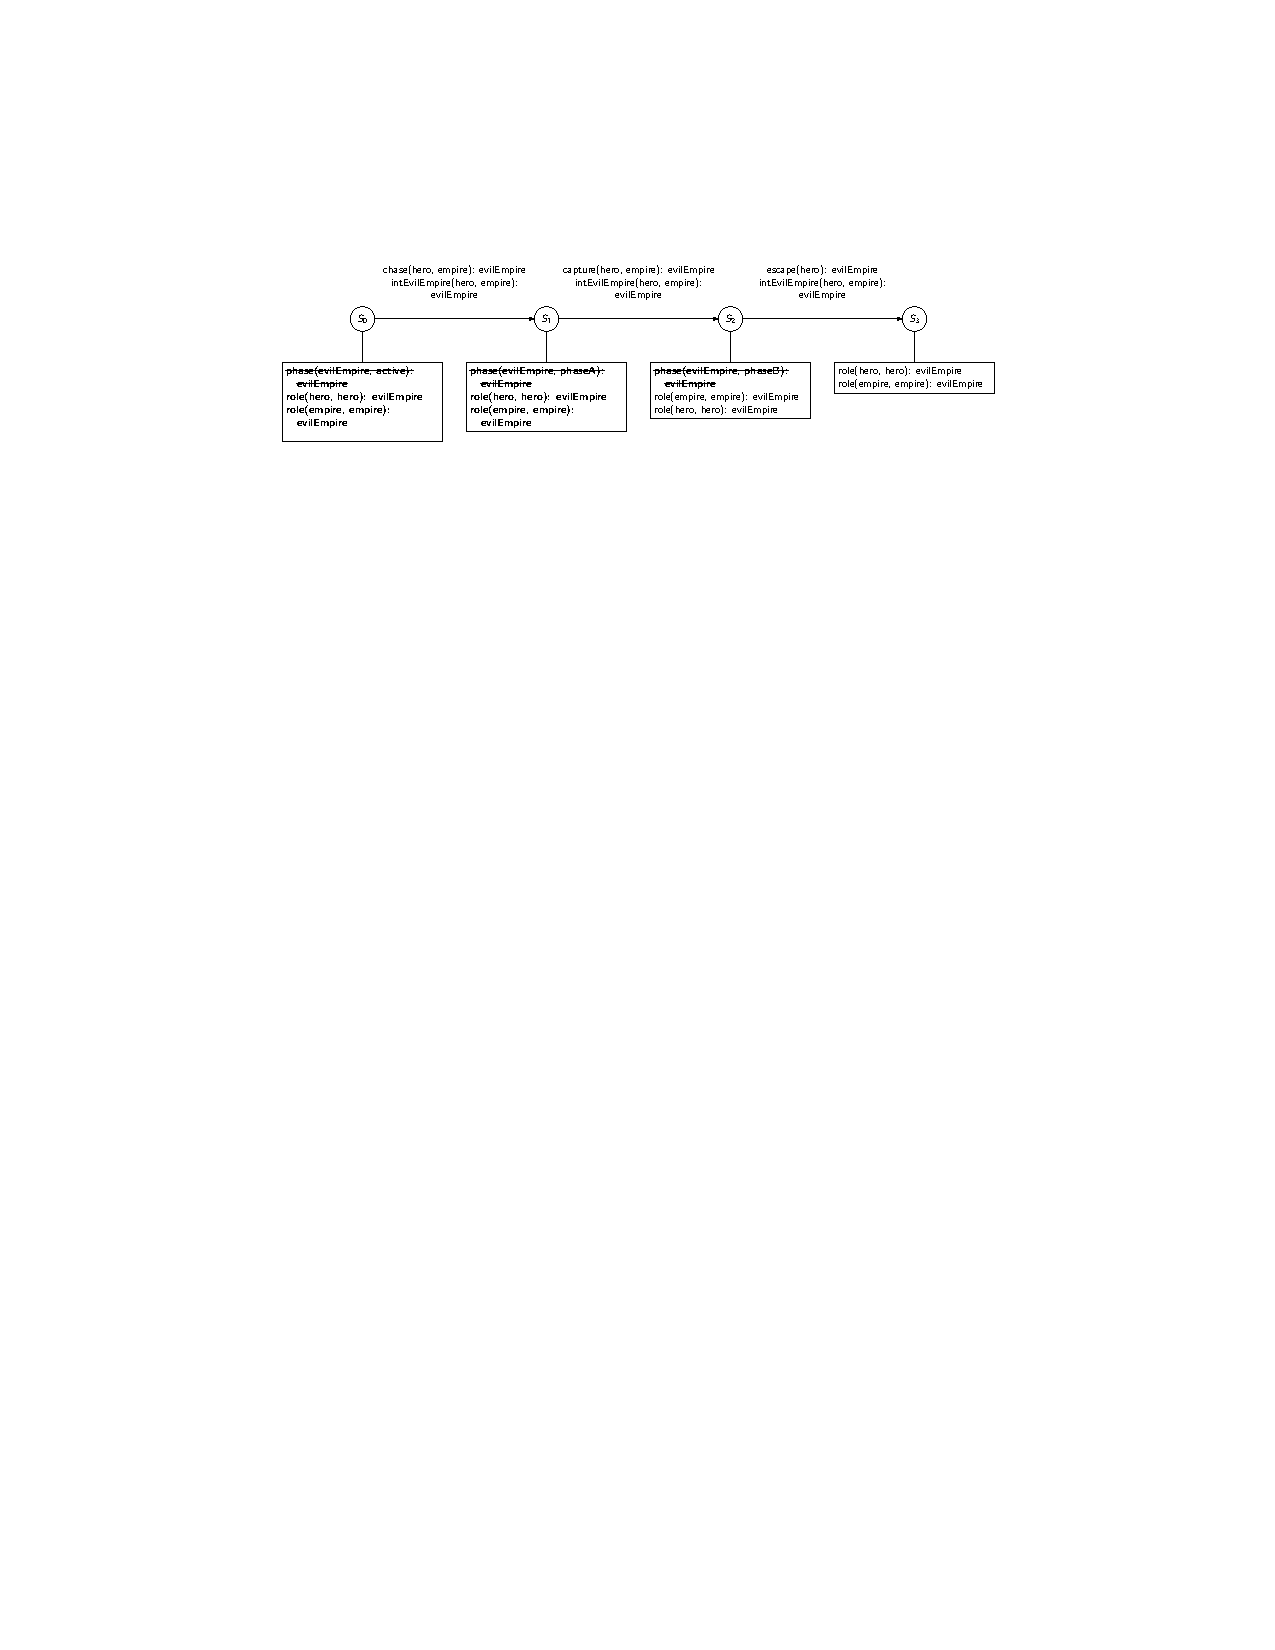
\includegraphics[width=\textwidth]{evilEmpire4-crop.pdf}}
\caption{Visualisation of the ``Evil Empire'' example trace in Listing~\ref{lst:evil-trace}}\label{fig:evil-trace}
\end{figure}

The events that appear at the start of the listing (starting with the
\emph{holdsat} predicate) on line~\ref{lne:as-holdsat} describe the \emph{fluents} that hold for a certain
institution at that particular time step in the answer set. After these
statements, the events that have \emph{occurred} in that institution appear.
These events can be both institutional or external events, which can be
distinguished due to the institutional event names beginning with ``int'' (such
as \emph{intEvilEmpire}, for example). External events usually trigger
institutional events with the institution name, which is why the \emph{chase} (line~\ref{lne:as-ex1}),
\emph{capture} (line~\ref{lne:as-ex2}) and \emph{escape} (line~\ref{lne:as-ex3}) events all trigger the \emph{intEvilEmpire}
institutional event on lines~\ref{lne:as-int1}, \ref{lne:as-int2} and~\ref{lne:as-int3} of Listing~\ref{lst:evil-trace}.

\subsection{The Hero's Journey}

\begin{lstlisting}[showstringspaces=false, escapechar=\~]
``The Hero's Journey'' is a trope where:
  The Hero is a role
  The Villain is a role
  Home is a place
  The Evil Lair is a place

  The Hero goes to the Evil Lair~\label{lne:hj-ev1}~
  Then the Hero kills the Villain~\label{lne:hj-ev2a}~
    Or the Villain escapes~\label{lne:hj-ev2b}~
  Then the Hero goes Home~\label{lne:hj-ev3}~
\end{lstlisting}

The answer set solver produces six traces for this trope. The branching
alternatives (the Hero can either kill the Villain or the Villain can escape at
one point in the trope) add an extra three answer sets to the output. If this
trope were just three events long, without the branching alternatives, then only
three answer sets would be produced (corresponding with stories of one, two
and three events long). The six answer sets are:

\begin{enumerate}
  \item Nothing happens
  \item The Hero goes to the Evil Lair
  \item The Hero goes to the Evil Lair, Then the Hero kills the Villain
  \item The Hero goes to the Evil Lair, Then the Hero kills the Villain, Then
    the Hero goes Home
  \item The Hero goes to the Evil Lair, Then the Villain escapes
  \item The Hero goes to the Evil Lair, Then the Villain escapes, Then the Hero
    goes Home
\end{enumerate}

The fourth answer set produced is shown in
listing~\ref{lst:hero-trace} as an example, and a visualisation appears in Figure~\ref{fig:hero-trace}.

\begin{lstlisting}[label={lst:hero-trace},caption={Example trace for the
``Hero's Journey'' trope}]
Answer Set 4:

Time Step 1:

holdsat(phase(herosJourney,phaseA),herosJourney)
holdsat(perm(kill(hero,villain)),herosJourney)
holdsat(perm(escape(villain)),herosJourney)
occurred(intHerosJourney(hero,villain,evilLair,home),herosJourney)
occurred(go(hero,evilLair),herosJourney)


Time Step 2:

holdsat(phase(herosJourney,phaseB),herosJourney)
holdsat(perm(go(hero,home)),herosJourney)
occurred(kill(hero,villain),herosJourney)
occurred(intHerosJourney(hero,villain,evilLair,home),herosJourney)


Time Step 3:

occurred(intHerosJourney(hero,villain,evilLair,home),herosJourney)
occurred(go(hero,home),herosJourney)
\end{lstlisting}


\begin{figure}[!t]
\centerline{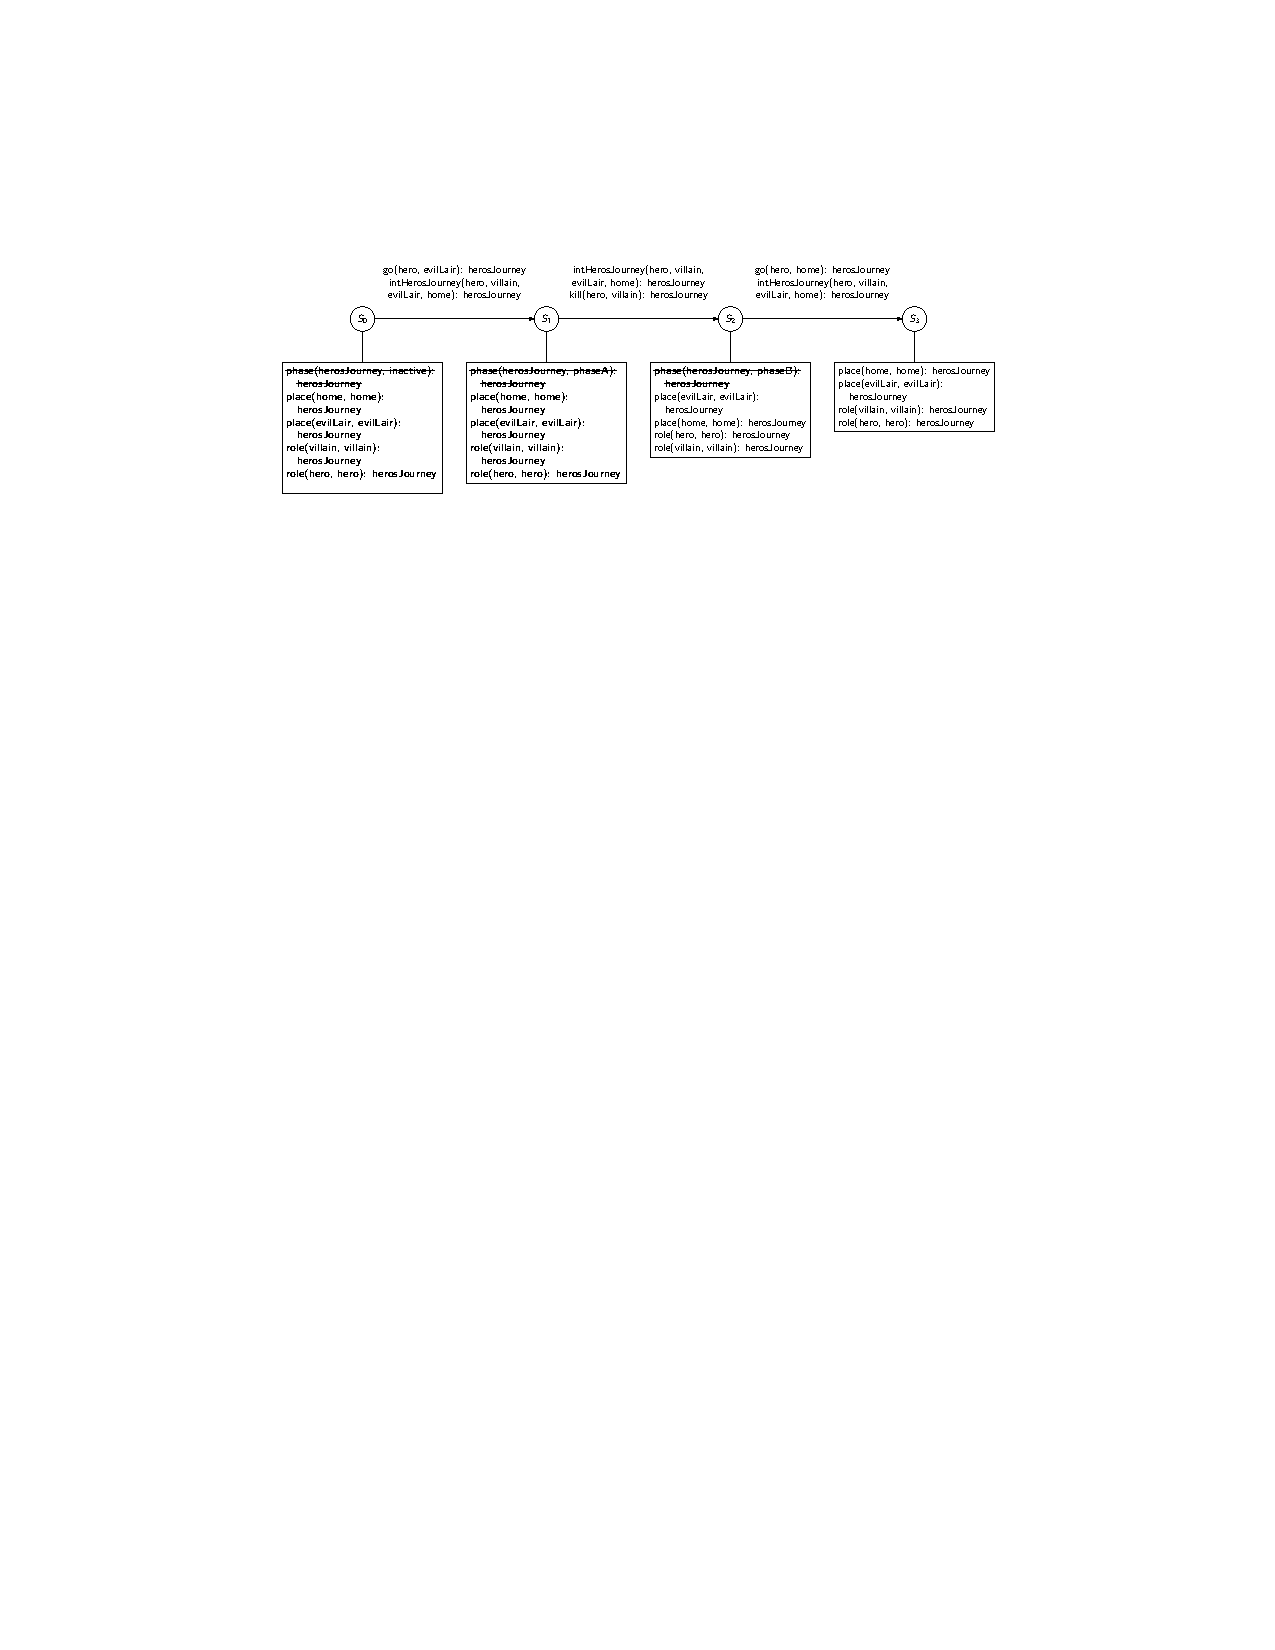
\includegraphics[width=\textwidth]{herosJourney4-crop.pdf}}
\caption{Visualisation of the ``Hero's Journey'' example trace in Listing~\ref{lst:hero-trace}}\label{fig:hero-trace}
\end{figure}

So far, the \emph{Evil Empire} and \emph{Hero's Journey} tropes produce
unremarkable results. Due to their simple natures, they only produce a small
number of answer sets when run through a solver. The results are more
interesting when both tropes are input into the solver, however.

\subsection{The Hero's Journey \emph{and} The Evil Empire}

Using both institutions as inputs into the solver, combining the two tropes, produces 124 answer sets. Combining the tropes in this case means
combining the sets of norms for both tropes in order to generate a branching
narrative. For example, if the first event of Trope A is ``The Hero goes Home'',
and the first event of Trope B is ``The Villain kills the Hero'', the
combination of both of these tropes gives both of these events permission to
happen. This means that the story can follow either Trope A or Trope B, adding
an extra element of nonlinearity to the story. Due to the fact that this offers
many different branching points in a story (where the story may follow either
one trope or another), the number of possible different stories increases
greatly, in this case to 124 different combinations.

Again, the reason that the solver produces so many answer sets is that it includes stories that
are less than the full length of every event from both tropes combined (which is
six events in this case). This is desirable when we are combining tropes, as
sometimes we need to incorporate events from a trope without needing it to run
its full course. In this example, if the Hero's Journey has come to an end, then
that would seem like a more suitable place to finish a story, rather than
waiting for all of the events in the Evil Empire trope to occur.

An example of a trace that runs the full six event length of both tropes put
together is shown in Listing~\ref{lst:hero-evil-trace} in
Appendix~\ref{appendix:full-trace}. A visualisation is shown in
Figure~\ref{fig:hjee-trace} in the same appendix.

These trace outputs do not assist the reader in visualising the possible
sequences of events that they represent. For this reason, we suggest that the
reader refer to the visualisations produced by the StoryBuilder tool in Section~\ref{sec:trope-visualisation}.

\subsection{Combining Tropes}
\label{sec:trope-combination-exp}
\added{
  This section describes an example of a situation where a user wants to combine
  multiple tropes together. There are two ways in which TropICAL and
  StoryBuilder allow this: by allowing tropes to happen ``at the same time'',
  and by sequencing tropes to occur at certain points in other tropes.
  Section~\ref{sec:subtrope-code} describes the use of subtropes in TropICAL,
  which are used to implement the latter case of sequencing tropes within
  scenes. Their implementation through institutional bridges is described in
  Section~\ref{sec:bridges}. This section examines how our system allows
  multiple tropes to occur at once.

  As an example, we can imagine that a user wants to use the following three
  tropes in their story: the \emph{Hero's Journey}, the \emph{Evil Empire} and
  the \emph{MacGuffin}. Using the StoryBuilder tool, the user can select all
  three tropes to occur at once using the dropdown menus in the ``arrange tab''
  (shown in Figure~\ref{fig:sb-combine-ann} on
  page~\pageref{fig:sb-combine-ann}). Alternatively, if not using StoryBuilder,
  the following code in Listing~\ref{lst:simultaneous-tropes} can be passed to
  the TropICAL compiler along with the trope definition files.

}{2.3.2b: Added a discussion on how to combine tropes}
  
\begin{lstlisting}[showstringspaces=false,
label=lst:simultaneous-tropes,caption={Simultaneous tropes in TropICAL}]
"Example Quest" is a scene where:
  The "Hero's Journey" trope happens
    And the "Evil Empire" trope happens
    And the "MacGuffin" trope happens
\end{lstlisting}

  Due to the fact that each trope is expressed as a sequence of permissions and
  obligations in an institution, a scene with multiple simultaneously active
  tropes means that multiple institutions are active at once. This gives each
  character the choice of participating in each institution in the order of
  their choice.

  Let us examine the ``Hero'' character role in this scene, for example. As all
  three trope institutions are active from the start of the scene, the character
  has permission to carry out the first event of any of the three tropes, as
  long as the permission applies to that character.
  Figure~\ref{fig:dot-combine1} shows an example where the first events of each
  institution permit the agent to perform an action, and so the agent is able to
  choose between these actions, in a similar manner to story branching.

  If the first event of the ``Hero's Journey'' trope is for the Hero to leave
  home, and the Hero does so, then the second event in the trope becomes
  permitted or obliged to occur, as shown in Figure~\ref{fig:dot-combine2}. Now
  we can see what happens if the Hero decides to follow the ``MacGuffin'' trope
  next: the second events of both the Hero's Journey and MacGuffin tropes become
  permitted, as well as the first event of the Evil Empire trope (as the Hero
  has not chosen an action that follows that trope yet).
  Figure~\ref{fig:dot-combine3} shows the situation after two choices from the Hero.

  A trope ends when its final event has occurred. The scene will end when either
  all the tropes have reached their points, or if the ``The story ends'' event occurs.

\begin{figure}[!h]
\centerline{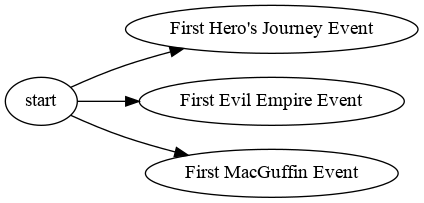
\includegraphics[width=0.6\textwidth]{combine1.png}}
\caption{An agent can choose between the events of all three tropes at the start
of the scene.}\label{fig:dot-combine1}
\end{figure}

\begin{figure}[!h]
\centerline{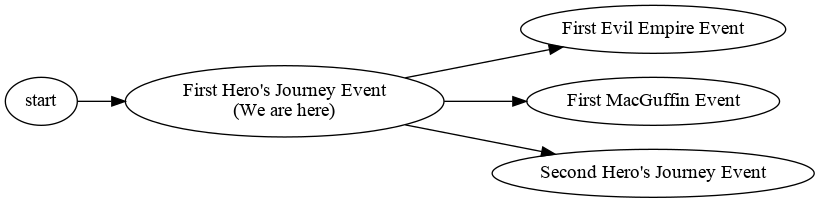
\includegraphics[width=\textwidth]{combine2.png}}
\caption{Now that the agent has chosen to perform the first event from the
  \emph{Hero's Journey} trope, the second event from that trope is now
  permitted, along with the first event of the other two tropes.}\label{fig:dot-combine2}
\end{figure}

\begin{figure}[!h]
\centerline{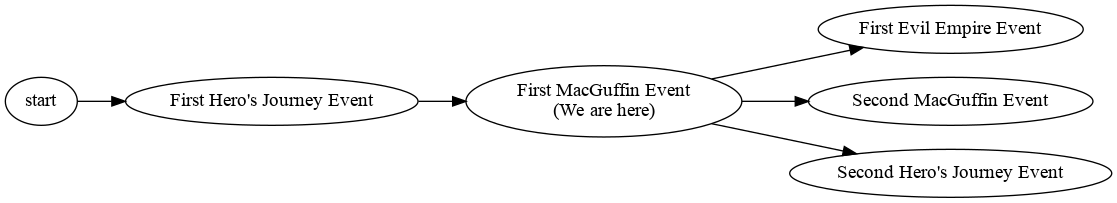
\includegraphics[width=\textwidth]{combine3.png}}
\caption{After following the \emph{Hero's Journey}, then the \emph{MacGuffin}
  tropes, there are still three paths for us to choose from.}\label{fig:dot-combine3}
\end{figure}

\section{Summary}
\label{sec:tropical-summary}
Returning to the requirements listed in Section~\ref{sec:requirements} (listed
again here for the reader's convenience), we can now examine our language
specification to see if the requirements are met:

\begin{enumerate}[R1.]
  \item \textbf{The software must be able to integrate into a
    multi-agent framework such as Jason}: The ``Punch and Judy'' example in Section~\ref{sec:punchjudy} describes
  how the normative framework of our system integrates with the Jason
multi-agent framework. The output of an answer set solver such as Clingo can be
used to add beliefs to an agent's mental model to let it know what actions it is
permitted and obliged to carry out as part of a story.
  \item \textbf{The system must direct the behaviour of agents to fit
    a story description}: 
The use of permissions and obligations to describe story actions to agents in
either a weakly (permissions) or strongly (obligations) enforced way gives the
author two ways to direct agent behaviour. At times when the author wants agents
to conform tightly with a trope description, they can give the agent an
obligation with a strict consequence for non-compliance.
  \item \textbf{The user should be able to write and re-use
    existing story components (from a library)}: Not addressed in TropICAL (see below).
  \item \textbf{The components must be able to express sequences of events}: Section~\ref{sec:seq-code} shows how sequences of events can be described in
TropICAL.
  \item \textbf{The components must be able to express branching
    (diverging) events}: Section~\ref{sec:branch-code} describes the
  implementation of branching story structures in TropICAL.
  \item \textbf{The user should have the ability to nest existing
    components inside new components}: This is an important feature of our
  language. Section~\ref{sec:subtrope-code} describes the
use of subtropes to meet the need for users to create their own abstractions.
  \item \textbf{The user should be able to visualise the branches of the
    story that result in the addition or modification of components to the
    story.}: Not addressed in TropICAL (see below).
  \item \textbf{The story must tell the character agents what to do, but
    they should be free to break away from it in extreme circumstances, to add a
    degree of unpredictability}: This is achieved
through the use of permissions to regulate agent actions.
\end{enumerate}

As a text-based programming language, TropICAL addresses the requirements
mentioned above (numbers~\ref{req:agents}, \ref{req:direct},
\ref{req:sequences}, \ref{req:branches}, \ref{req:subtropes} and
\ref{req:norm}). However, there are two requirements that cannot be fulfilled
through a text-based programming paradigm alone: selecting pre-existing story
components from a library (requirement~\ref{req:components}), and visualising
the branches of the story as it is modified (requirement~\ref{req:vis}). These
requirements are best addressed through an Interactive Development Environment
(IDE) with which we can add graphical features for the browsing, selection and
visualisation of tropes. The next chapter (Chapter~\ref{cha:storybuilder})
introduces \emph{StoryBuilder}, a browser-based tool that adds these features to
our TropICAL language.

% TODO outro: 1

% storybuilder

% HACK: predicted poms remaining: 51

\chapter{StoryBuilder: An Interface for Trope-based Interactive Story Creation}
% Think of it as an IDE: what kind of support do users want? Helps to visualise the complexity of the stories. Helps authors to construct the stories that they intend to construct
\label{cha:storybuilder}

Though TropICAL is useful as a programming language that allows for the
construction of stories using controlled natural language, there remain several
barriers that would prevent its use by non-programmer story authors. It is
implemented as a compiler that is invoked from a command line interface with one
or more trope definitions as input. Its output is a set of InstAL institutions
and the AnsProlog that these institutions compile to. The AnsProlog can then be
input into the Clingo solver in order to produce answer sets
that correspond to the set of all possible story paths. This interface presents
the following challenges to non-programmers:

\begin{itemize}
  \item Users must be familiar with command-line tools
  \item Users must know how to use the Clingo solver
  \item Users must be able to parse and understand the answer sets that Clingo produces
\end{itemize}

These challenges would be difficult for a non-technical story author to
overcome. Therefore, we offer StoryBuilder as a graphical user interface to enhance the usability of
the TropICAL language. In addition to removing the barriers to TropICAL's use
listed above, it addresses requirements
R\ref{req:components} and R\ref{req:vis} in the requirements listed in Section~\ref{sec:requirements}:

\begin{enumerate}[R1.]
  \setcounter{enumi}{2}
  \item The user should be able to write and re-use
    existing story components (from a library)
  \setcounter{enumi}{6}
  \item The user should be able to visualise the branches of the
    story that result from the addition or modification of components to the story.
\end{enumerate}

These requirements suggest the implementation of an IDE (Interactive Development
Environment) with visual tools that assist the selection and visualisation of
tropes. StoryBuilder is designed to be an IDE that is specifically designed for
trope-based story authoring. It takes the form of a graphical user interface
that runs in a web browser, sends snippets of TropICAL code to a server to be
compiled and input into Clingo, and visualises the resulting answer sets.

Although libraries can be stored and reused in text-based programming languages
through methods such as ``import'' statements, our intention is to create a
graphical interface to simplify the exploration and viewing of tropes in the
library. Using StoryBuilder, the user can select a pre-written trope from a
dropdown box of existing tropes, which then allows them to see its source code
and visualise its structure in the story with a tree diagram.

To address requirement~\ref{req:vis}, we parse the answer set outputs (traces)
of our answer set solver (as described in Section~\ref{sec:trope-visualisation}) to create a tree
diagram of all of the possible events that they describe.

\section{Interface}

% TODO intro: 1
% TODO description of interface: 2
% TODO screens & explanation of editor: 2
% TODO screens & explanation of arranger: 2
StoryBuilder is implemented as a web application with client (browser-based)
and server components. The client, developed in the ClojureScript programming
language~\citep{clojurescript} and compiled to Javascript, consists of the graphical user interface
with which the user creates, selects and visualises tropes. The client passes
TropICAL code to the server (written in Clojure~\citep{clojure}), which compiles
the code to InstAL and runs the resulting AnsProlog code through the
\emph{clingo} answer set solver. The resulting answer sets are then passed back
to the client as hash map data structures, which are then visualised as graph diagrams.

The following sections provide an overview of StoryBuilder's user interface,
explaining how it can be used for the creation, arrangement and visualisation of tropes.

\subsection{Overview}

\begin{figure}[!ht]
\centerline{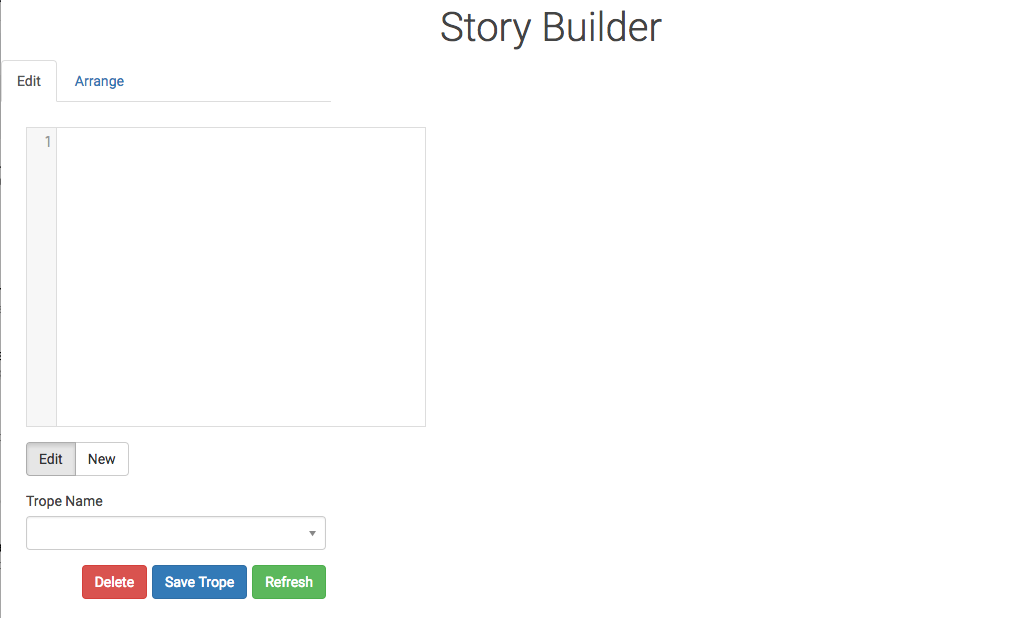
\includegraphics[width=\textwidth]{storybuilder5.png}}
\caption{The initial view when \emph{StoryBuilder} starts}\label{fig:sb-start}
\end{figure}

Figure~\ref{fig:sb-start} shows what the user sees when they first start the
\emph{StoryBuilder} tool. On the left side of the screen are two tabs:
\emph{edit} and \emph{arrange}. The \emph{edit} tab allows the user to edit
existing tropes, or to create a new trope of their own. While editing these
tropes, their structures are visualised on the right side of the screen (which
is blank in this initial screenshot). Figure~\ref{fig:sb-edit-ann} shows the
same screen as Figure~\ref{fig:sb-start}, with the addition of annotations that
explain the function of each item in the interface.

\begin{figure}[!ht]
\centerline{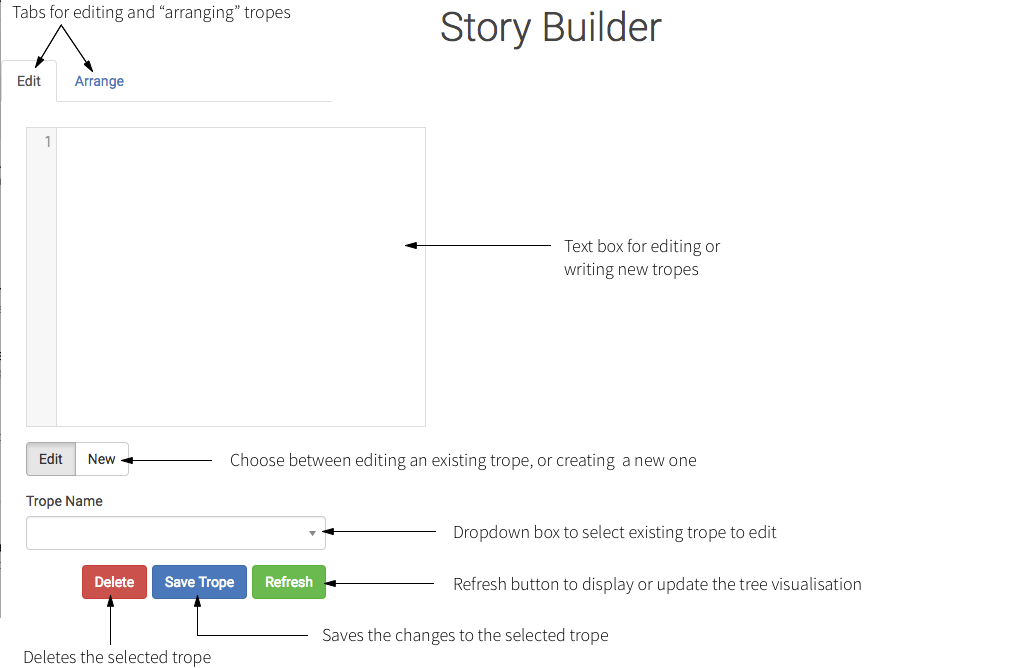
\includegraphics[width=\textwidth]{storybuilder-a1.png}}
\caption{An explanation of the \emph{edit} tab}\label{fig:sb-edit-ann}
\end{figure}

\subsubsection{The \emph{edit} tab}
To edit a trope that has been created previously, the user selects it from a
list of tropes in the dropdown box at the bottom-left of the screen. This causes
the trope's text to appear in the text editor that occupies most of the
left-hand portion of the screen. From here, the user may amend the text in the
editor, and click the blue \emph{save trope} button to make the changes persist.
The user may also click the red \emph{delete} button to remove the trope from
the database.

\begin{figure}[!ht]
\centerline{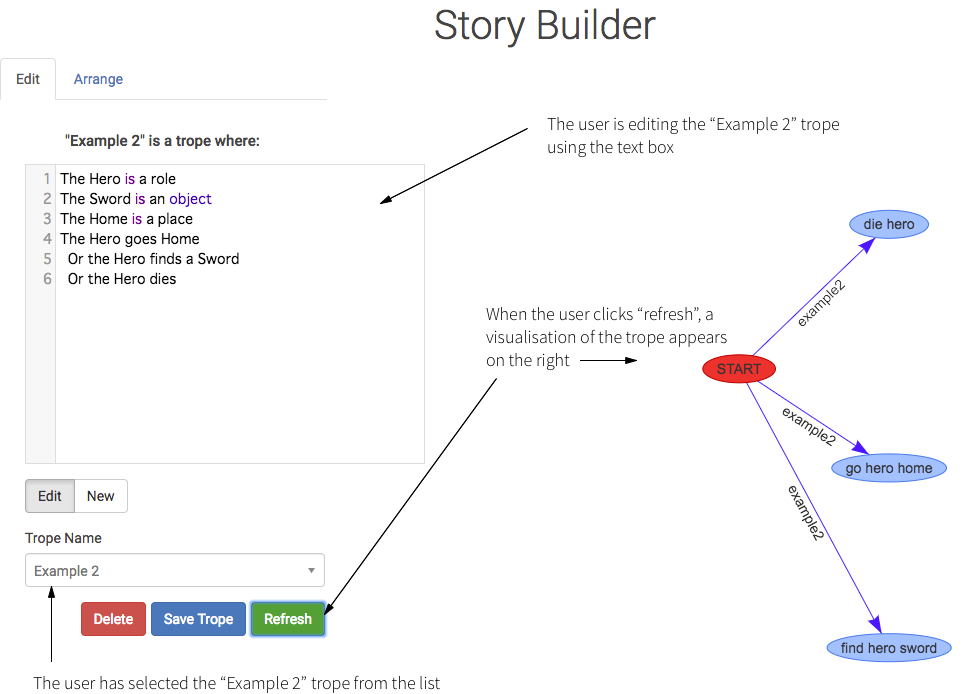
\includegraphics[width=\textwidth]{storybuilder-a2.png}}
\caption{An explanation of how the \emph{edit} tab is used}\label{fig:sb-edit-ann2}
\end{figure}

If the user selects a trope and then, at some point, clicks the green
\emph{refresh} button, a visualisation of its path structure appears on the
right side of the screen. An example visualisation appears in
figure~\ref{fig:sb-edit-ann2}, with annotations that further explain the features
of the interface in the \emph{edit} tab.

\begin{figure}[!ht]
\centerline{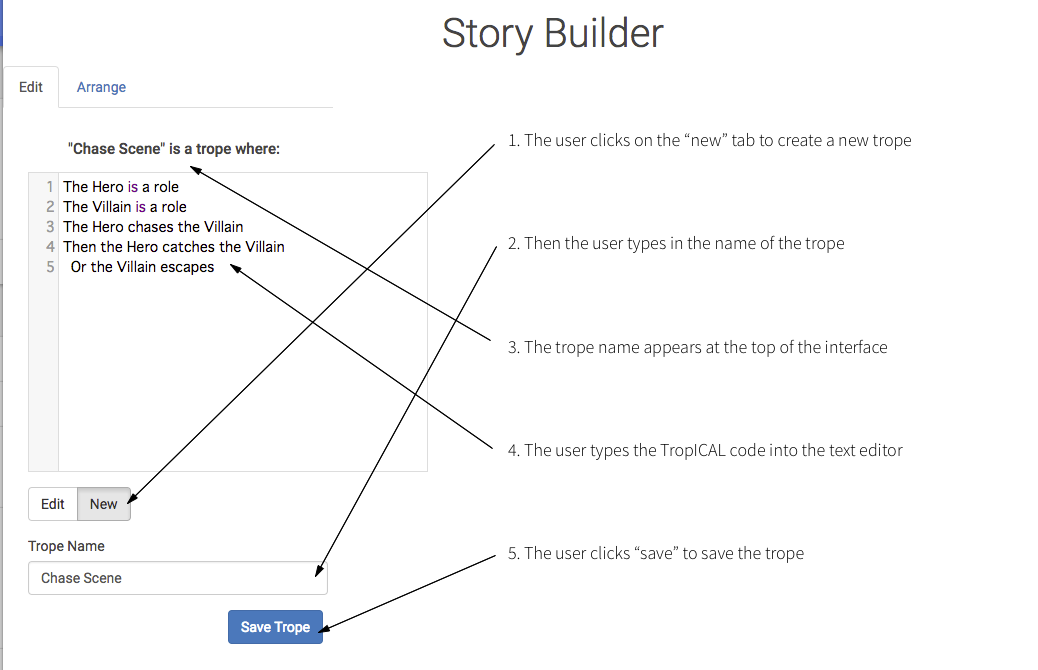
\includegraphics[width=\textwidth]{storybuilder-new1.png}}
\caption{An explanation of how a new trope is created}\label{fig:sb-new-ann}
\end{figure}

The user also uses the interface in the \emph{edit} tab to create a new trope.
Figure~\ref{fig:sb-new-ann} shows the five steps that a user must take in order
to create a trope:

\begin{enumerate}
  \item The user clicks on the ``new'' tab below the text area to create a new trope
  \item The user types the name of the trope into the text box below the main
    text area (and below the ``new'' tab that they have just clicked on).
  \item The trope name appears at the top of the interface as the first line of
    the \emph{TropICAL} trope. For example, for a trope named ``Chase Scene'',
    the line above the text area will appear as: \emph{``Chase Scene'' is a
      trope where:}. The system prompts the user if the name is already in use.
  \item The user types the TropICAL code into the main text area
  \item The user clicks on the blue ``save'' button at the bottom of the screen
    to save the trope.
\end{enumerate}

Once a trope is created, then the user may return to the \emph{edit} tab to
select and visualise it.


\subsubsection{Trope Visualisation}
\label{sec:trope-visualisation}
The tree visualisation that appears on the right side of the \emph{StoryBuilder}
interface is produced from the output of running the \emph{clingo} answer set
solver on the AnsProlog translation of the trope being edited. The output,
which we refer to as \emph{answer sets} or \emph{traces} in Section~\ref{sec:t-asp}, are lists of events that are possible in one run
through the story. \emph{Clingo} outputs one answer set for each possible
interpretation of the events that can occur in a story. Examples of these traces
are explained further in Section~\ref{sec:example-traces}.

These traces are converted into a tree data structure by merging all events that
occur at the same time step with the same predecessor events into one node. This
eliminates redundant paths in the visualisation, reducing the visual clutter and
making it easier for the author to understand. This data structure is used as
the input to \emph{vis.js}\footnote{Accessible at the following website:
  \url{http://visjs.org}, accessed 20170826.}, a Javascript library for graph visualisation. This
library draws the tree on an interactive canvas on screen, allowing the user to
drag the nodes around and zoom in on them.

In the visualisation, each node is labelled with an event in
\emph{verb_subject_object} prefix notation. For example, a node corresponding to
``The Hero goes to the Land of Adventure'' would be labelled as
\emph{``go_hero_landOfAdventure''}. The reason for this labelling is to reduce
the verbosity of the original controlled natural language statement in order to
convey the essential information inside a graph node. The edges between
each node are labelled with the name of the trope that corresponds to the event with the
later time step. For example, if
Event A is an \emph{Evil Empire} trope event and is followed by Event B, a
\emph{Hero's Journey} event, the edge linking the nodes together will be
labelled with Event B's trope (\emph{The Hero's Journey}). In order to allow for
easier visual identification of the different story paths that different tropes
allow, the edge for each trope has a unique colour, with Trope A's lines
appearing in blue, Trope B's being red, and Trope C's being green, for example.

\subsubsection{The \emph{arrange} tab}

The \emph{arrange} tab allows the user to combine multiple tropes into a story,
and to visualise all the possible paths through that story.

\begin{figure}[!th]
\centerline{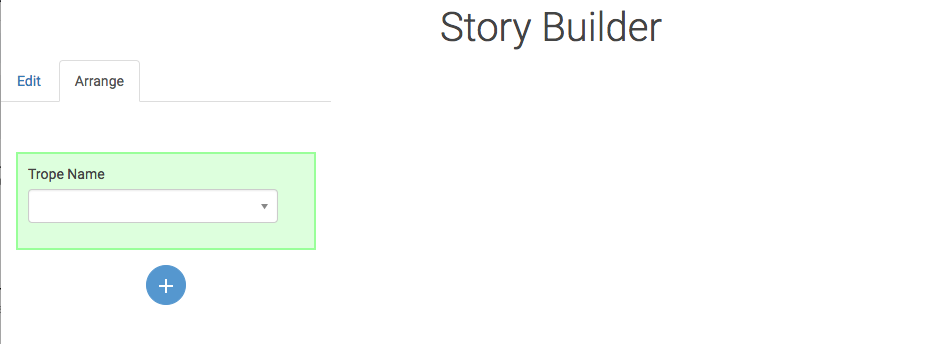
\includegraphics[width=\textwidth]{storybuilder6.png}}
\caption{The view when the user clicks the \emph{arrange} tab}\label{fig:sb-arrange}
\end{figure}

Figure~\ref{fig:sb-arrange} shows the view that the user sees when the
\emph{arrange} tab is first clicked. The screen appears mostly blank, with the
exception of a green rectangle on the left side of the screen, where the user
may select from a list of pre-written tropes. The user may select extra tropes
by clicking on the blue plus (``+'') symbol below the green box.

Once one or more tropes are selected, a tree visualisation appears on the right
side of the screen to show the combination of paths that a story may take, based
on the selected tropes. Figure~\ref{fig:sb-combine-ann} shows the steps that a
user takes to combine tropes together in the interface, along with a part of the
visualisation that appears as a result of selecting two example tropes. In order
to combine multiple tropes together in this way, a user must go through these steps:

\begin{figure}[!th]
\centerline{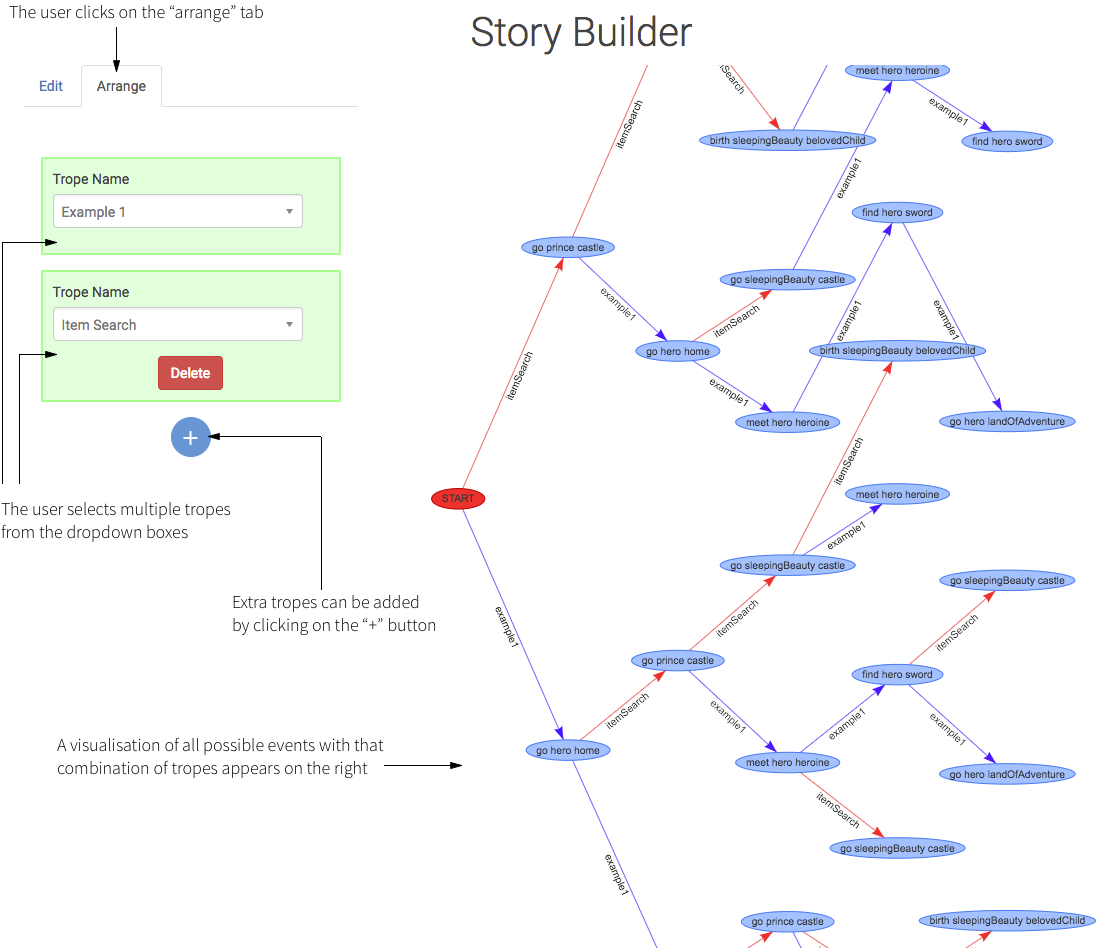
\includegraphics[width=\textwidth]{storybuilder-combine1.png}}
\caption{An explanation of tropes are combined in the \emph{arrange} tab}\label{fig:sb-combine-ann}
\end{figure}

\begin{samepage}
\begin{enumerate}
  \item The user clicks on the ``arrange'' tab at the top-left of the screen
  \item The user selects a trope from the dropdown box inside the green rectangle
  \item The user waits for the resulting visualisation to appear
  \item The user clicks on the blue ``+'' symbol below the selected trope on the left
  \item The user selects another trope from the dropdown box that has just appeared
  \item The user waits for the resulting visualisation to appear
\end{enumerate}
\end{samepage}

A particularly important feature of the visualisation is that each graph edge is
labelled with the name of the trope that links two events. In the example
shown in Figure~\ref{fig:sb-combine-ann}, events that follow the \emph{Example
  1} trope are connected with a red arrow, and events that follow the \emph{Item
Search} trope are connected with a blue arrow. This allows the user to see
the effect adding a certain trope has on the potential paths that their story
may take.


\begin{figure}[!t]
\centerline{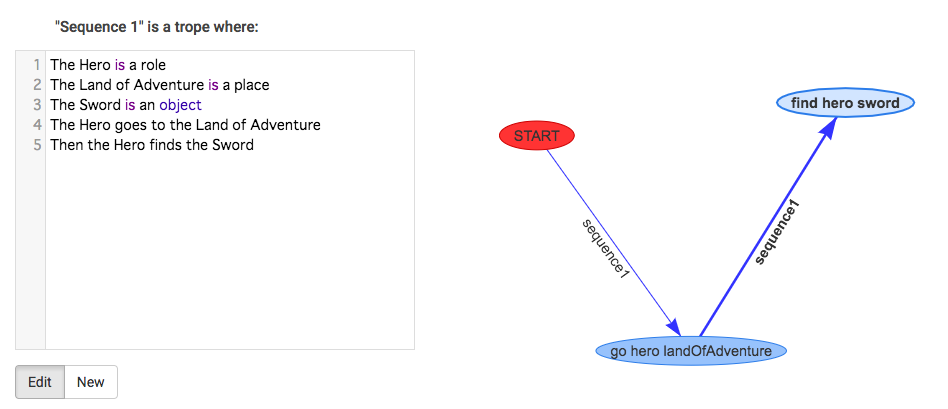
\includegraphics[width=\textwidth]{storybuilder-seq1.png}}
\caption{Two consecutive events (from Listing~\ref{lst:seq2})}\label{fig:sb-seq1}
\end{figure}

\begin{figure}[!t]
\centerline{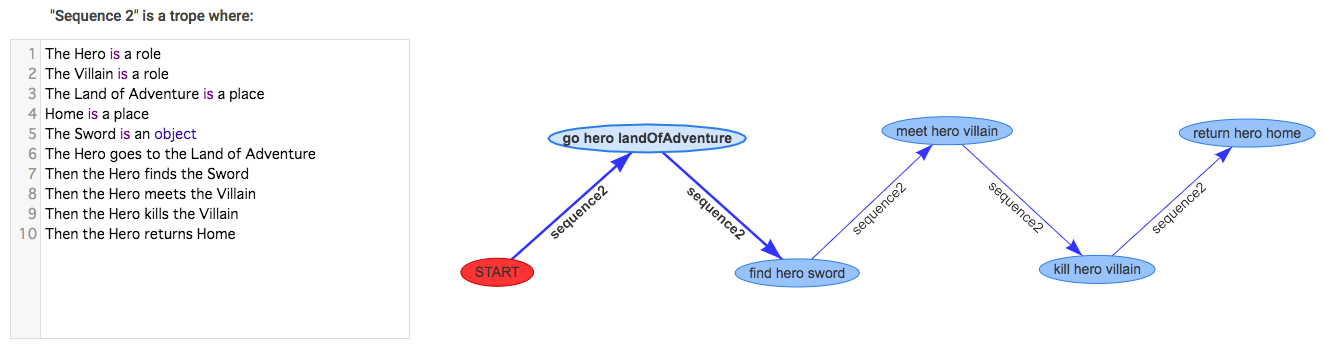
\includegraphics[width=\textwidth]{storybuilder-seq2.png}}
\caption{A sequence of events (from Listing~\ref{lst:seq4})}\label{fig:sb-seq2}
\end{figure}

\subsection{Usage Examples}

The figures in this section show how the simple trope examples listed in Sections~\ref{sec:seq-code}
to~\ref{sec:subtrope-code} appear when edited and visualised using the
\emph{StoryBuilder} tool.

\begin{figure}[!t]
\centerline{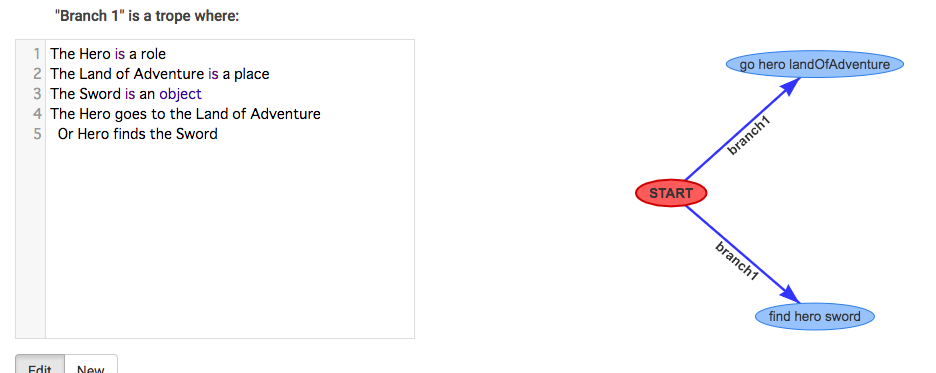
\includegraphics[width=\textwidth]{storybuilder-branch1.png}}
\caption{Two branches (from Listing~\ref{lst:branch1})}\label{fig:sb-branch1}
\end{figure}

\begin{figure}[!t]
\centerline{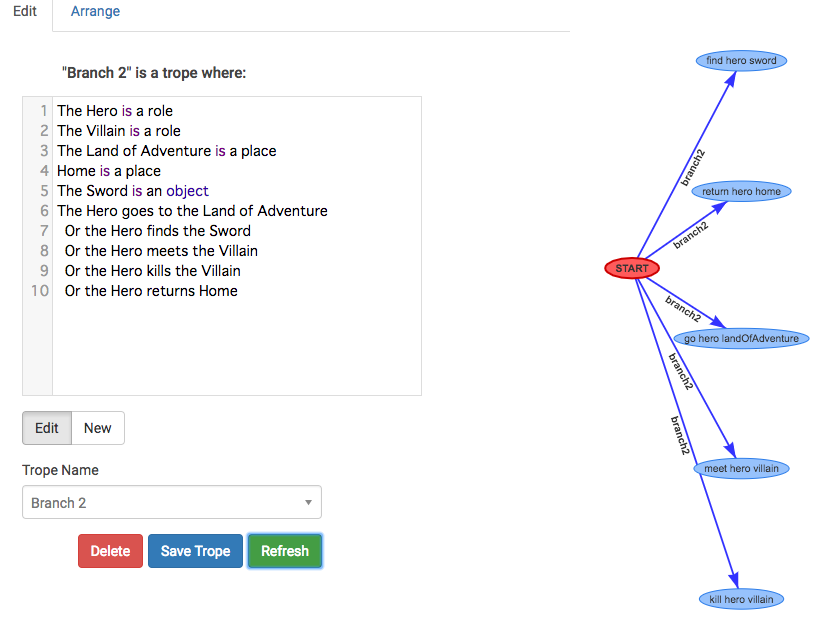
\includegraphics[width=\textwidth]{storybuilder-branch2.png}}
\caption{Five branches (from Listing~\ref{lst:branch2})}\label{fig:sb-branch2}
\end{figure}

To demonstrate the visualisation of sequences of events,
figure~\ref{fig:sb-seq1} shows a sequence just two events long, with the code
from Listing~\ref{lst:seq2} as input. Figure~\ref{fig:sb-seq2} uses the longer
sequence of five events from Listing~\ref{lst:seq4} as its input.

\emph{StoryBuilder}'s visualisation of branches are demonstrated in the figures
that follow. Figure~\ref{fig:sb-branch1} shows the simple two-branch trope of
listing~\ref{lst:branch1}. Figure~\ref{fig:sb-branch2} shows the visualisation
of a trope with five different branches, as described by the trope in
listing~\ref{lst:branch2}. Finally, the more complicated combination of
sequences and branches from Listing~\ref{lst:branch3} is shown in Figure~\ref{fig:sb-branch3}.

\begin{figure}[!t]
\centerline{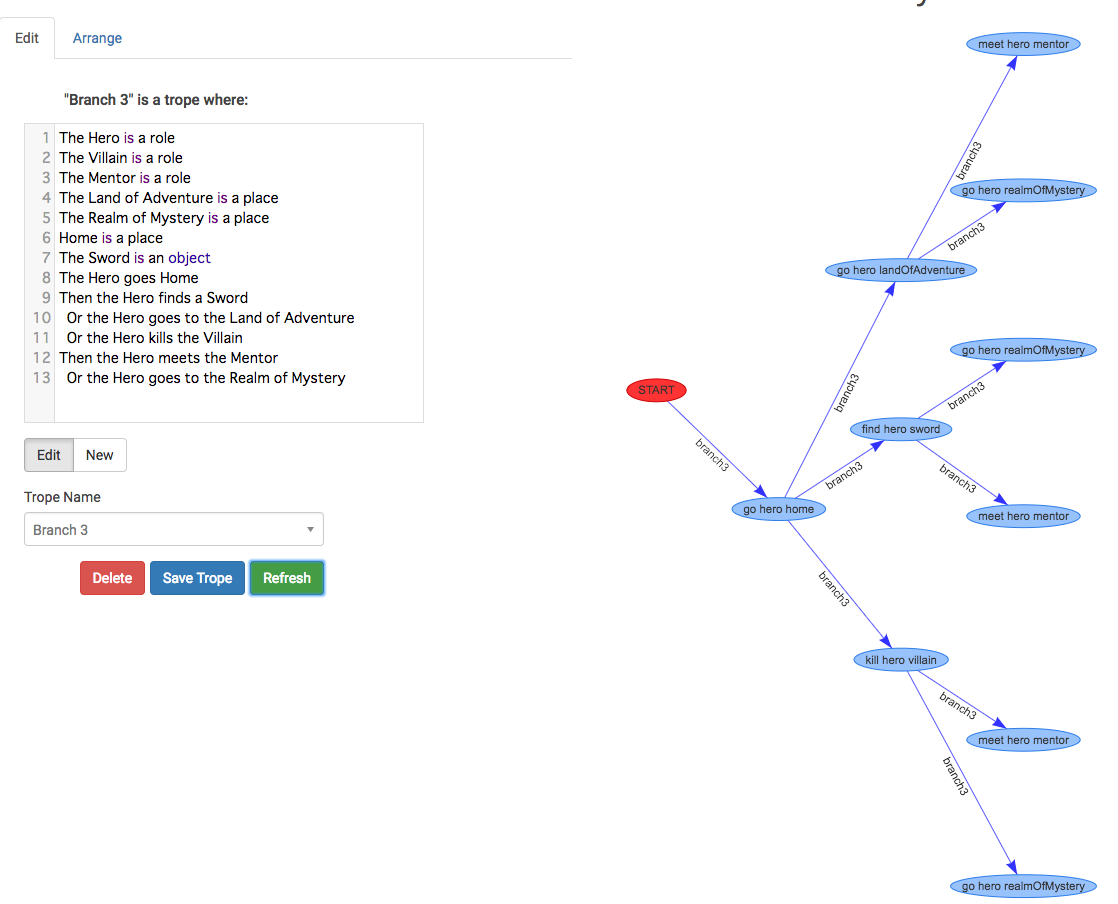
\includegraphics[width=\textwidth]{storybuilder-branch3.png}}
\caption{A combination of branches and sequences (from Listing~\ref{lst:branch3})}\label{fig:sb-branch3}
\end{figure}


\begin{figure}[!t]
\centerline{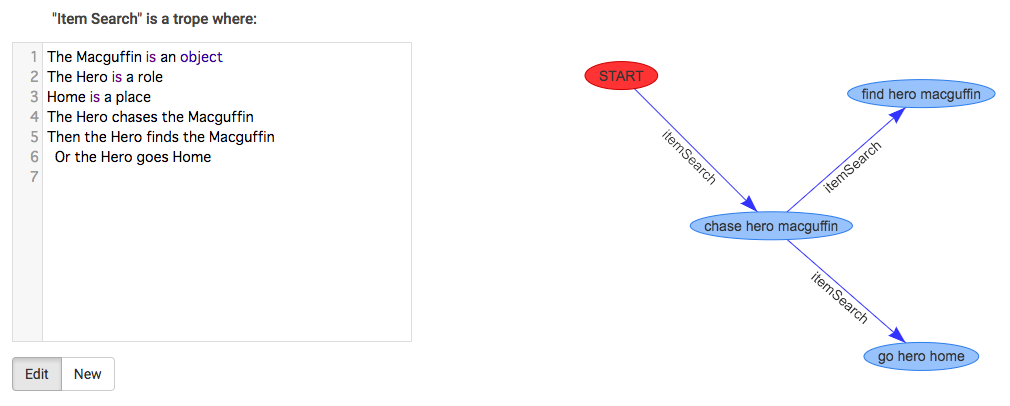
\includegraphics[width=\textwidth]{storybuilder-subtrope1.png}}
\caption{Subtrope to be embedded (from Listing~\ref{lst:subtrope1})}\label{fig:sb-subtrope1}
\end{figure}


The final two figures in this section demonstrate the use of \emph{StoryBuilder}
for embedding subtropes inside of other tropes. Figure~\ref{fig:sb-subtrope1} is
the \emph{StoryBuilder} visualisation that corresponds to the subtrope that is
to be embedded (described in Listing~\ref{lst:subtrope1}). The actual embedding
of this subtrope, as described in Listing~\ref{lst:subtrope2}, and its resulting visualisation are shown in Figure~\ref{fig:sb-subtrope2}.

\begin{figure}[!t]
\centerline{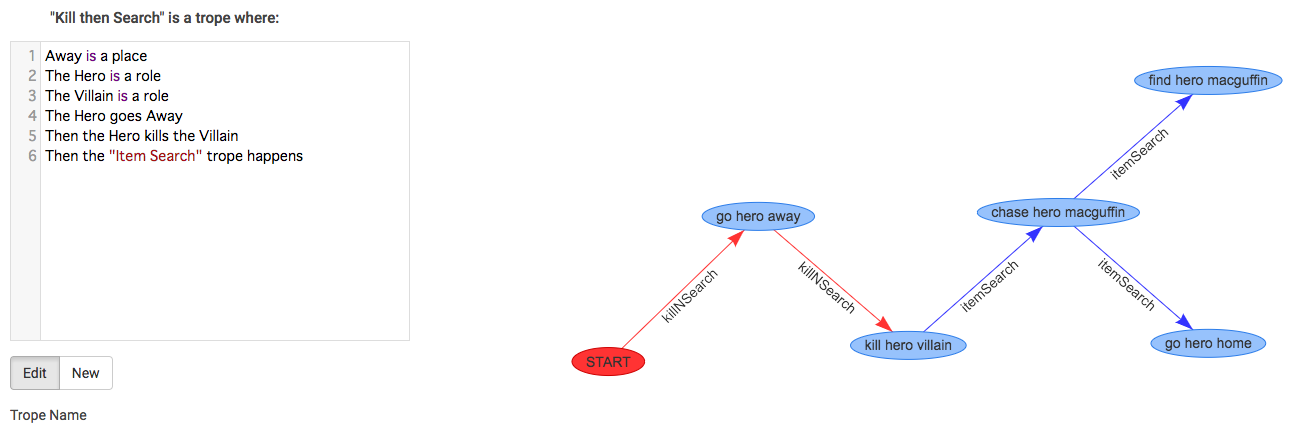
\includegraphics[width=\textwidth]{storybuilder-subtrope2.png}}
\caption{Trope containing a subtrope (from Listing~\ref{lst:subtrope2})}\label{fig:sb-subtrope2}
\end{figure}

\subsection{Introducing ``Punch and Judy''}
\changed{}{Moved this back here from its previous position in Ch.\ref{cha:institutions}, as this is now the first mention of P\&J}

From this point in the thesis, we use the \emph{Punch and Judy} story world for our
example narratives. \emph{Punch and Judy} is a traditional British-Italian
puppet show often seen at seaside resorts. Its first recorded appearance in the
UK is in Covent Garden, London in 1662, having been brought into the country by
Italian puppeteer Pietro Gimonde. Since then it has become a British cultural
institution, delighting children and adults alike over the course of centuries.

The show itself is an incredibly violent farce, where the titular character
\emph{Punch} is a homicidal maniac with a hair-trigger temper. Most scenes start
with him having an argument with another puppet, and end with Punch beating the
other puppet to death. He starts by killing his wife and child, then the
policeman that comes to arrest him, before finally murdering the Devil himself.

Interestingly, there is no comeuppance for Punch's killing spree, as most modern
audiences would expect. Instead, the story shows Punch as a buffoon, a
ridiculous caricature of an angry man who blunders his way through life, yet is
victorious nonetheless. The story has no moral message, only farcical violence.

Despite its arguable nihilism, \emph{Punch and Judy} has many features that make
it a suitable narrative domain for the purposes of testing our research:

\begin{itemize}
\item It has many recognisable patterns, or \emph{tropes}. For example, most
  scenes feature some kind of audience participation, and most end with
  slapstick comedy.
\item It can be as simple or sophisticated as we choose to make it. Some scenes
  are relatively simple to model, such as the scene where Punch beats the
  policeman. Others are more difficult, such as where Punch is asked to guard
  some suasages, but then loses them to a crocodile. Combining several scenes
  into a complete and recognisable \emph{Punch and Judy} narrative is, we
  contend, a worthwhile challenge for a narrative generation system.
\item Following from this, its scenes can either be self-contained and modelled
  on their own, or can depend on the context of the previous scenes. For
  example, Punch's foes increase in importance as his rampage progresses. In some
  versions, he kills his wife, then a policeman, then the executioner sent to
  hang him, then finally the Devil. This makes it useful for modelling a
  narrative with a state that changes over time.
\item Most (British) people know Punch and Judy when they see it. They are able
  to recognise how characters in the story are supposed to behave, and what
  should happen in each scene and in the story as a whole. This helps with
  evaluation of the system: the audience will be able to say whether or not the
  generated tropes are \emph{authentic} or not.
\end{itemize}

The minimal set of Punch and Judy characters would be Punch, his wife Judy,
their baby, Joey the clown (who narrates the story and interacts with the
audience, and is immune to Punch's attacks), a crocodile and a Policeman.
Extended versions include other animals that Punch chases (such as a monkey or
cat), and the previously mentioned hangman and Devil characters. These are not
needed for a full Punch and Judy show, however. Indeed, many performers show
just one or two scenes in a show, with the first featuring Punch, Judy and the
baby, and then finishing with the scene where Punch wrestles with a crocodile
for some sausages.

\subsection{Creating a Punch and Judy story with StoryBuilder}
The tropes that appear in Punch and Judy can be divided into two types: those
that are present throughout the story, and those that describe particular scenes
of the story. One trope that is a constant feature of Punch and Judy shows is
audience participation, where the characters shouts something at the audience
with the expectation of a response. For example, the Punch character may shout
something like: ``Where is he?'', with the traditional audience response being
``He's behind you!''.

There are also particular scenes that always feature in a Punch and Judy show.
The two scenes that we will describe are the ``Babysitting scene'', where Judy leaves Punch with the
Baby, and the ``Crocodile Sausages'' scene, where a crocodile eats some sausages
that Punch has been trusted with looking after.

\begin{figure}[!t]
\begin{lstlisting}[label={lst:audience-participation},caption={The ``Audience participation'' trope}]
``Audience Participation'' is a trope where:
The Character is a role
The Audience is a role
The Character shouts at the Audience
Then the Audience shouts at the Character
\end{lstlisting}

\smallskip

\centerline{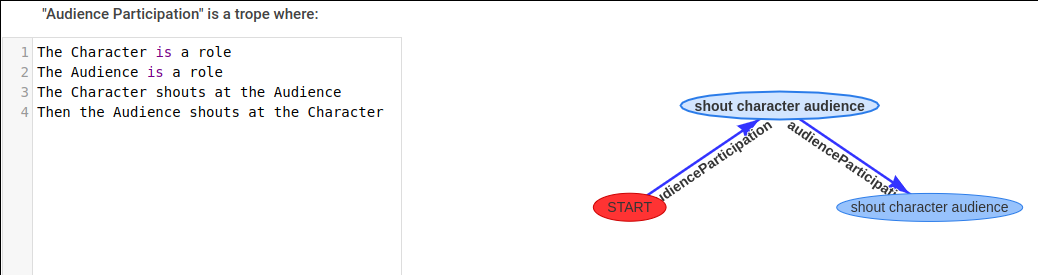
\includegraphics[width=\textwidth]{audience-trope.png}}
\caption{The ``Audience Participation'' trope in StoryBuilder}\label{fig:audience-participation}
\end{figure}

Listing~\ref{lst:audience-participation} shows a basic description of the events
that happen in audience participation: a character calls out to the audience,
then the audience calls back. When integrated into a multi-agent system, each
character agent will be assigned the ``character'' role, so that the social
norms from this trope will apply to them.
Figure~\ref{fig:audience-participation} shows how this trope appears when it is
input into StoryBuilder.

Because this trope is present throughout the Punch and Judy story, it can be
either inserted as a subtrope into other tropes, or (perhaps more effectively)
passed to the answer set solver along with the other tropes in the story, so
that its events can occur at any point. This is done via the ``arrange'' tab in
the user interface, described in Section~\ref{sec:combining-tropes} below.

Listing~\ref{lst:babysitting-trope} shows a trope to describe the
``Babysitting'' scene from Punch and Judy. We have decided to put a branching
point in this trope, where Punch may either kill the baby, or the baby escapes.
This gives the option of a more ``family-friendly'' alternative of the scene,
suitable for younger audiences. The StoryBuilder visualisation appears in Figure~\ref{fig:babysitting-trope}.

\begin{figure}[!t]
\begin{lstlisting}[label={lst:babysitting-trope},caption={The ``Babysitting'' trope}]
``Babysitting'' is a trope where:
  Punch is a role
  Judy is a role
  The Baby is a role
  Away is a place
  Home is a place
  Judy kisses Punch
  Then Judy goes Away
  Then Punch chases the Baby
  Then Punch kills the Baby
    Or the Baby escapes
  Then Judy returns Home
\end{lstlisting}

\smallskip
\centerline{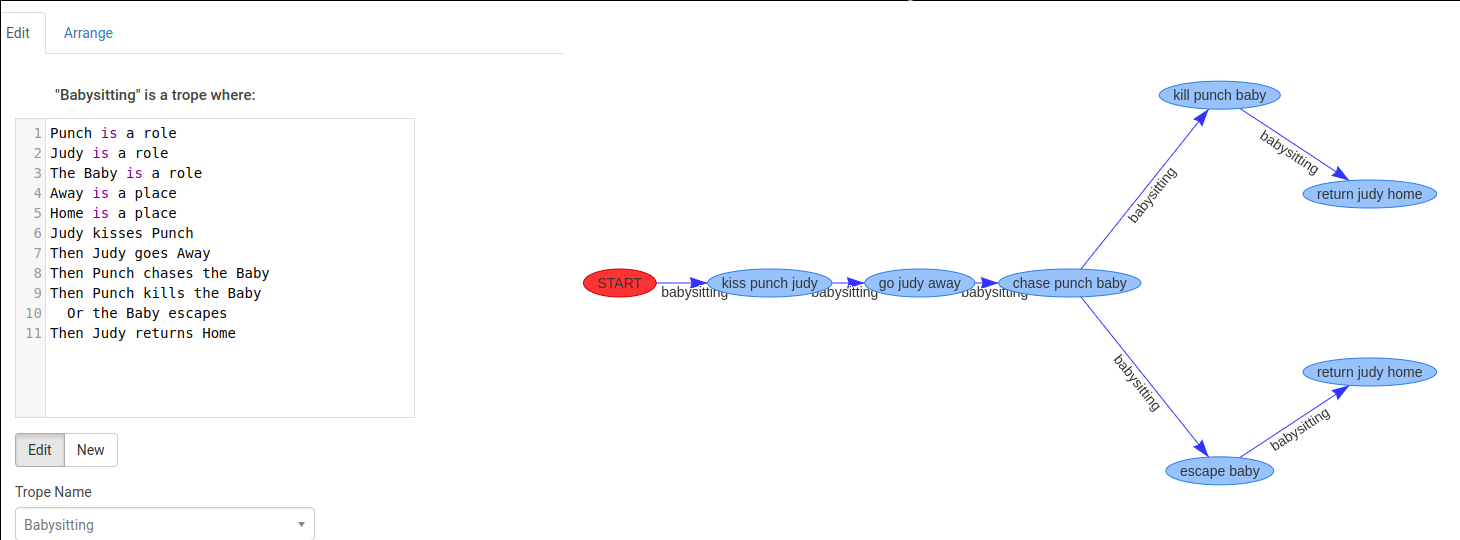
\includegraphics[width=\textwidth]{babysitting-trope.png}}
\caption{The ``Babysitting'' trope in StoryBuilder}\label{fig:babysitting-trope}
\end{figure}

Listing~\ref{lst:sausages-trope} shows the TropICAL definition of the
``Crocodile Sausages'' scene in Punch and Judy. This scene is a simple sequence
of events, but we will see how to interpose events from other tropes between
them below. Its StoryBuilder visualisation appears in Figure~\ref{fig:crocodile-sausages}.

\begin{figure}[!t]
\begin{lstlisting}[label={lst:sausages-trope},caption={The ``Crocodile Sausages'' trope}]
``Crocodile Sausages'' is a trope where:
  Punch is a role
  Joey is a role
  Crocodile is a role
  The Sausages are an object
  Away is a place
  Home is a place
  Joey meets Punch
  Then Joey leaves behind the Sausages
  Then Joey goes Away
  Then the Crocodile appears
  Then the Crocodile chases Punch
  Then the Crocodile eats the Sausages
  Then Joey returns Home
\end{lstlisting}

\smallskip
\centerline{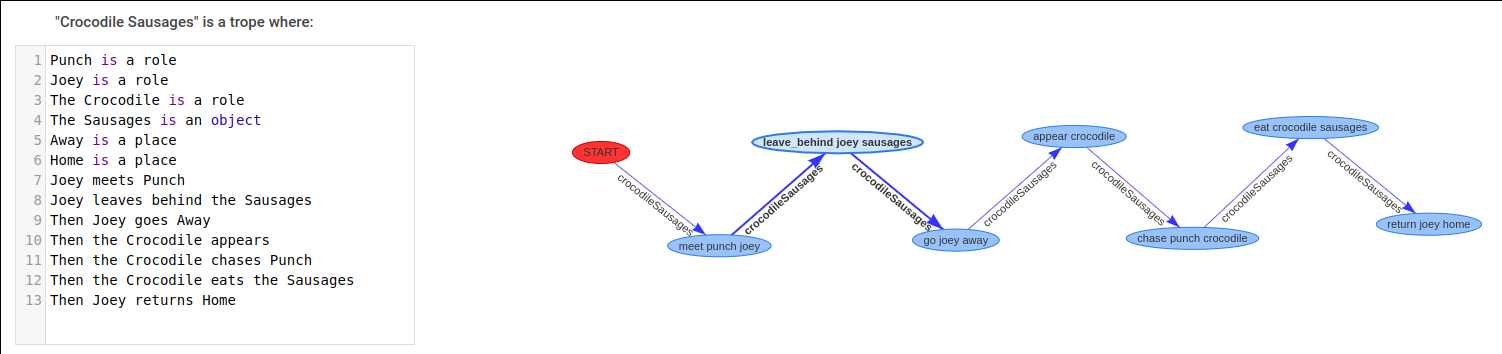
\includegraphics[width=\textwidth]{crocodile-trope.png}}
\caption{The ``Crocodile Sausages'' trope in StoryBuilder}\label{fig:crocodile-sausages}
\end{figure}

However, these tropes can be further simplified and modularised. Both the
``Babysitting'' and ``Crocodile Sausages'' feature events where a character
leaves the stage, only to return later. With this knowledge, we can abstract
these events into the ``Absentation'' trope, shown in
listing~\ref{list:absentation-trope}.

\begin{minipage}{\textwidth}
\begin{lstlisting}[label={list:absentation-trope},caption={An ``Absentation'' trope}]
``Absentation'' is a trope where:
  Absentee is a role
  Home is a place 
  Away is a place
  The Absentee goes Away
  Then the Absentee returns Home
\end{lstlisting}
\end{minipage}

Similarly, many Punch and Judy scenes end
with two characters chasing each other, such as when the Crocodile chases Punch,
or the scene where the Policeman chases Punch. From this, we can create the
``Chase Scene'' trope of Listing~\ref{list:chase-trope}.

\begin{minipage}{\textwidth}
\begin{lstlisting}[label={list:chase-trope},caption={A ``Chase Scene'' trope}]
``Chase Scene'' is a trope where:
  Pursuer is a role
  Pursued is a role
  The Pursuer chases the Pursued
  Then the Pursuer catches the Pursued
    Or the Pursued escapes
\end{lstlisting}
\end{minipage}

Creating these new abstractions allows us to rewrite our tropes without
repeating ourselves. Listing~\ref{list:babysitting-trope-subtrope} shows how the
``Babysitting'' trope would be rewritten by incorporating the ``Absentation''
and ``Chase Scene'' tropes as subtropes.
Listing~\ref{list:sausages-trope-subtrope} does the same for the ``Sausages'' trope.

\begin{minipage}{\textwidth}
\begin{lstlisting}[label={list:babysitting-trope-subtrope},caption={The ``Babysitting''
trope, redefined with a subtrope}]
``Babysitting'' is a trope where:
  Punch is a role
  Judy is a role
  The Baby is a role
  Away is a place
  Home is a place
  Judy kisses Punch
  Then the ``Absentation'' trope happens
  Then the ``Chase Scene'' trope happens
\end{lstlisting}
\end{minipage}

\begin{minipage}{\textwidth}
\begin{lstlisting}[label={list:sausages-trope-subtrope},caption={The ``Sausages''
trope, redefined with a subtrope}]
``Sausages'' is a trope where:
  Punch is a role
  Joey is a role
  Crocodile is a role
  The Sausages are an object
  Away is a place
  Home is a place
  Joey gives the Sausages to Punch
  Then the ``Absentation'' trope happens
  Then the Crocodile appears
  Then the Crocodile chases Punch
  Then the Crocodile eats the Sausages
  Then Joey returns Home
\end{lstlisting}
\end{minipage}

A full 

\subsection{Combining Tropes Together}
\label{sec:combining-tropes}

\begin{figure}[!t]
\centerline{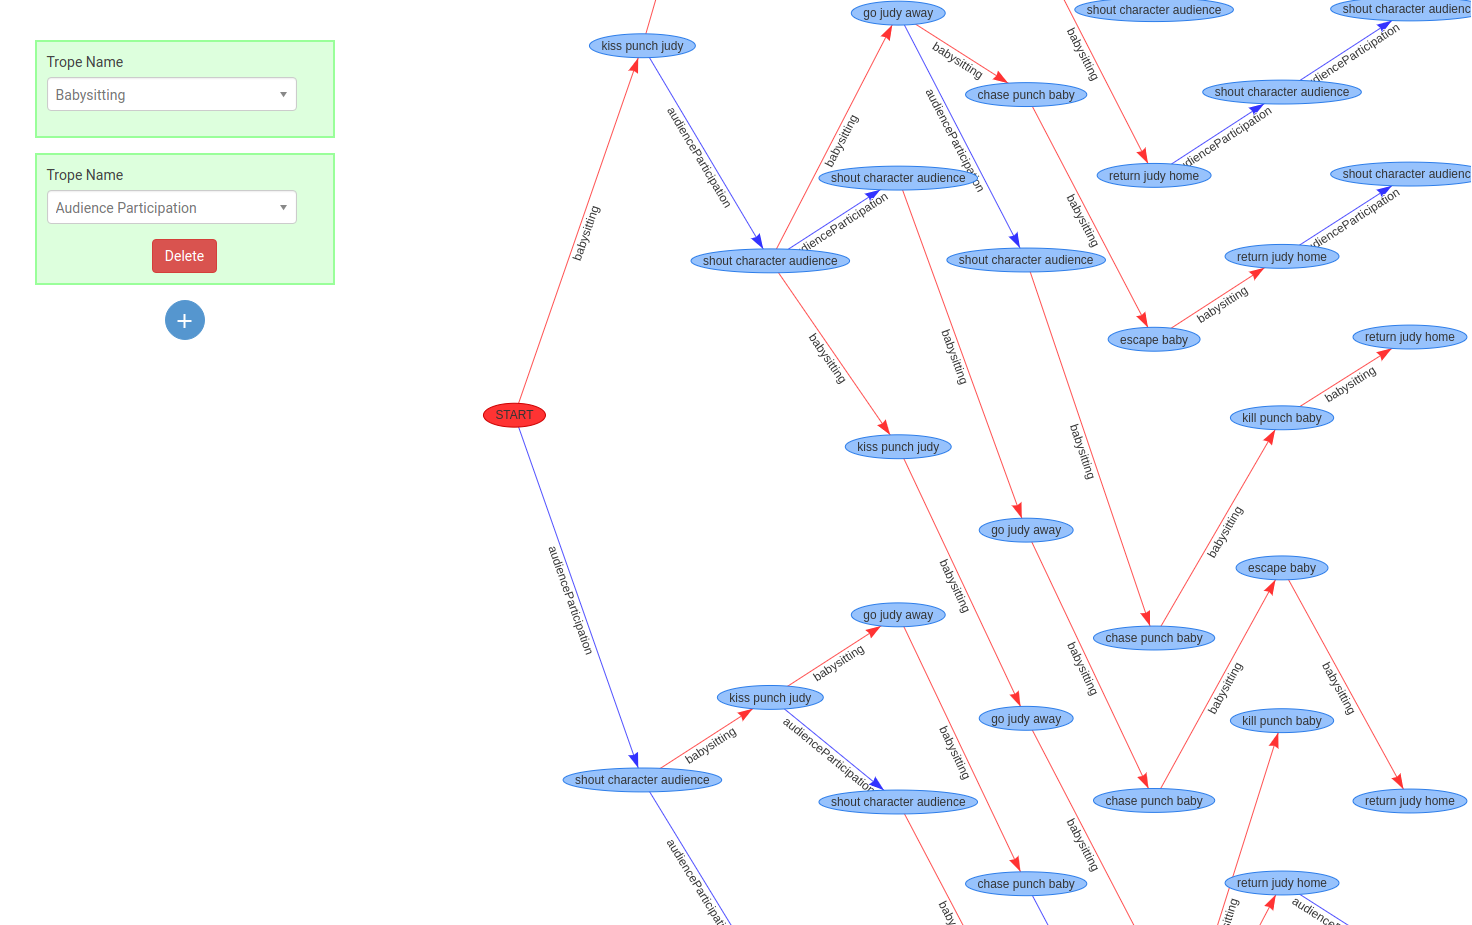
\includegraphics[width=\textwidth]{trope-combining.png}}
\caption{Combining the ``Babysitting'' and ``Audience Participation'' tropes in StoryBuilder}\label{fig:combining-tropes}
\end{figure}

Sometimes we want to combine two or more tropes together into a story, so that
the characters are free to choose to follow the events of any of the tropes that
may be happening. In this example, we describe a scene where the events of the
``Babysitting'' scene are combined with the ``Audience Participation'' trope.
This would mean that both tropes are active at the same time, allowing the
characters to perform the actions described in both tropes.

Using the ``arrange'' tab in StoryBuilder, we select both the ``Audience
Participation'' and ``Babysitting'' tropes. The tree visualisation that appears
on the right of the screen shows us all of the permutations that appear as the
output of the answer set solver. Figure~\ref{fig:combining-tropes} shows the
result of doing this in StoryBuilder. The tree visualisation on the right has
been enlarged so that its nodes are legible. The nodes of the tree describe the
events that are occurring, and the links between nodes are labelled with the
name of the trope that their following nodes (events) correspond to.

This has the effect of ``mixing'' the events of the two tropes together. Example
sequences of events in a scene with both the ``Babysitting'' and ``Audience
Participation'' tropes would be:

\begin{enumerate}
\item Judy kisses Punch (\emph{Babysitting})
\item A Character (Judy or Punch) shouts at the Audience (\emph{Audience Participation})
\item Then Judy goes away (\emph{Babysitting / Absentation})
\item Then Punch chases the Baby (\emph{Babysitting / Chase Scene})
\item The Audience shouts at a Character (Punch) (\emph{Audience Participation})
\item Then the Baby escapes (\emph{Chase Scene})
\item Then Judy returns Home (\emph{Babysitting / Absentation})
\end{enumerate}

This corresponds to one of the permutations of combining the events of the
``Babysitting'' and ``Audience Participation'' tropes in different orders, and
would be just one of the many paths through the visualised tree.

Using this part of the StoryBuilder tool, the user is able to interactively
explore the different combinations of events that different tropes add to their
story. When these combinations of tropes are visualised, they are then able to
refine their tropes further in order to build the non-linear narrative that they desire.

\added{Further discussion on trope combination appears in Section~\ref{sec:trope-combination-exp}.}{2.3.3: Forward ref to discussion on
  combining tropes together}

\section{Design Justification}
% Return to requirements, explain how they are met

% TODO intro: 1
% TODO explain how requirements have been met: 4

In the introduction to this chapter, we describe how the StoryBuilder tool
addresses requirements R\ref{req:components} and R\ref{req:vis} in the
requirements shown in section~\ref{sec:requirements}:

\begin{enumerate}[R1.]
  \setcounter{enumi}{2}
  \item The user should be able to write and re-use
    existing story components (from a library)
  \setcounter{enumi}{6}
  \item The user should be able to visualise the branches of the
    story that result in the addition or modification of components to the story.
\end{enumerate}

StoryBuilder fulfills requirement R\ref{req:components} by storing every trope
that the author creates in a database, so that they may be reused and amended if
needed. Requirement R\ref{req:vis} is met through StoryBuilder's use of a tree
visualisation that updates as the story author is editing the tropes in the tool.

\section{Evaluation}
\label{sec:sb-eval}
% TODO intro: 2

In order to evaluate the effectiveness of both TropICAL and StoryBuilder for the
construction of tropes and nonlinear stories, we carried out a usability study,
evaluated qualitatively through a thematic analysis (described
by~\citet{clarke2014thematic}, and in Section~\ref{sec:sb-analysis}).

The StoryBuilder tool is not integrated into a multi-agent system. This is due
to its focus on story structure design and visualisation using tropes, rather
than for the creation of the character agents themselves. For this reason, the
analysis is not designed to evaluate requirements~\ref{req:agents},
\ref{req:direct} and~\ref{req:norm} from Section~\ref{sec:requirements}, only
those related to the use of tropes for story construction:

\begin{enumerate}[R1.]
  \setcounter{enumi}{2}
  \item The user must be able to write and re-use
    existing story components (from a library)
  \item The components must be able to express sequences of
    events
  \item The components must be able to express branching
    (diverging) events
  \item The user must have the ability to nest existing
    components inside new components
  \item The user must be able to visualise the branches of the
    story that result in the addition or modification of components to the
    story
\end{enumerate}

Additionally, the study aims to examine the user experience of using tropes to
construct stories in StoryBuilder with the following supplemental requirements:

\begin{enumerate}[S1.]
  \item\label{req:tropes-natural} To evaluate the suitability of TropICAL's controlled natural language
    syntax for non-programmer story authors
  \item\label{req:tropes-reusable} To examine the use of tropes as reusable story components
  \item\label{req:tropes-abstractions} To see if tropes allow a natural means of creating abstractions of story patterns
  \item\label{req:tropes-vis} To study whether the story tree visualisations
    generated from the answer set solver output assists in non-linear story creation
\end{enumerate}

These requirements are difficult to measure compared to those described in
Section~\ref{sec:requirements}, and so are used as the basis of the questions
asked throughout the thematic analysis:

\begin{itemize}
  \item How easy or difficult did you find the language to learn? (Requirement~\ref{req:tropes-natural})
  \item Could you create the story you wanted by combining tropes together? (Requirement~\ref{req:tropes-reusable})
  \item Were you able to create the abstractions you wanted using subtropes? (Requirement~\ref{req:tropes-abstractions})
  \item Did the visualisations assist you in the creation of tropes and stories? (Requirement~\ref{req:tropes-vis})
\end{itemize}

The aim of the thematic analysis is to identify themes that emerge from the participants' answers to these questions.

\subsection{Procedure}
% TODO explain the process: 3

The study begins with a brief explanation of the syntax and features of the
TropICAL language: entities (roles, places, objects), events (sequences and
branches) and subtropes. Once they have become familiar with the language and
seen some visualisations of example tropes, they are asked to complete seven
tasks. The tasks start with the user making simple changes to existing tropes,
and give the user increasing freedom, finally giving them the opportunity to
create tropes for a story of their own. Detailed descriptions of the tasks are
given in Section~\ref{sec:user-tasks}.

\subsection{Participants}
Eight participants were recruited for the study:

\begin{itemize}
\item \textbf{Participant A} is a computer science student,
with good programming experience
\item \textbf{Participant B} is an architect and former English teacher with a little programming experience
\item \textbf{Participant C} is a creative writer with no programming experience
\item \textbf{Participant D} is a computer science student with good programming experience
\item \textbf{Participant E} is a computer science student with good programming experience
\item \textbf{Participant F} is a creative computing student with some programming experience
\item \textbf{Participant G} is a computer scientist that works on well-known
interactive fiction tools
\item \textbf{Participant H} is a computer science graduate student with good
programming (and answer-set programming) experience
\end{itemize}

The studies were conducted using Google Hangouts, with each participant loading
StoryBuilder by going to a web address
(\url{http://mthompson.org/storybuilder}) and sharing a screen capture of their
interactions with the system. Each study was recorded using screen capture
software. The full transcripts, with annotations, are listed in
Appendix~\ref{appendix:transcripts}.

\subsection{User Tasks}
\label{sec:user-tasks}
This section describes the tasks that the users carried out as part of the study.

\subsubsection*{Task 1: Edit an Existing Trope}
\label{sec:org14aee76}
The user is instructed to get a feel for the language by browsing through
the examples provided, then presented with this task:

\begin{framed}
\begin{quote}
In the 'edit' tab, select an existing trope from the dropdown box. Edit its text on the left, and then save it. Once this is done, check to see that the visualisation seems to be as expected.
\end{quote}
\end{framed}

This task is designed to examine how easily the user is able to read and
understand the TropICAL languages before making small changes to existing
tropes, testing requirement R\ref{req:components}.

\subsubsection*{Task 2: Create a Trope}
\label{sec:org96a6276}

The second task gives the user some specific character roles and places to use
in their trope, and then instructs them to combine them together into a sequence
of events:

\begin{framed}
\begin{quote}
Given the following character roles:

\begin{itemize}
\item Hero
\item Villain
\item Mentor
\end{itemize}

And the following places:

\begin{itemize}
\item Home
\item Evil Lair
\item Land of Adventure
\end{itemize}

Construct a trope using Tropical. Your statements will be simple sequences at first, i.e:

\begin{verbatim}
The Hero goes home
Then the Hero goes away
Then the Villain kills the Hero
\end{verbatim}

Make sure to declare your roles and objects first.
\end{quote}
\end{framed}

This task is designed to allow the users to gently begin creating their own
tropes, by limiting their role and place choices at first, as well as limiting
their trope complexity by only allowing sequences of events without branches.
This also tests requirements R\ref{req:components} and R\ref{req:sequences}.

\subsubsection*{Task 3: Adding objects to your trope}
\label{sec:org9cb2b36}

This task extends task 2 by allowing the user to add objects to their trope.

\begin{framed}
\begin{quote}
Add the following objects to your trope:

\begin{itemize}
\item Weapon
\item Evil Plan
\end{itemize}

For example:

\begin{verbatim}
The Hero takes the Weapon
Then the Villain makes an Evil Plan
\end{verbatim}
\end{quote}
\end{framed}

\subsubsection*{Task 4: Add branches to your trope}
\label{sec:org80c0de6}

In task 4, the user is asked to add some branching points to the trope that they
have made:

\begin{framed}
\begin{quote}
Using the "Or" keyword, add branches to your story. For example:


\begin{verbatim}
The Hero goes to the Land of Adventure
Then the Hero kills the Villain
  Or the Villain kills the Mentor
  Or the Mentor goes home
\end{verbatim}
\end{quote}
\end{framed}

This task introduces the concept of branches to the user for the first time,
testing requirement R\ref{req:branches}.

\subsubsection*{Task 5: Put two tropes into a story}
\label{sec:orga5afeae}

In this task, the user takes two existing tropes from the database, and combines
them together with the ``arrange'' tab:

\begin{framed}
\begin{quote}
Using the "Arrange" tab in Storybuilder, select two (or more) tropes from the dropdown boxes to visualise all the possible paths through a story with those tropes.
\end{quote}
\end{framed}

Once this task is completed, the user is able to see a visualisation of all of the possible
combinations of events that result from combining two tropes together. This task
tests requirement R\ref{req:vis}.

\subsubsection*{Task 6: Tropes within Tropes}
\label{sec:orga5bc382}

This task introduces the user to the concept of a \emph{subtrope}, asking them
to embed an existing trope inside of a new one:

\begin{framed}
\begin{quote}
Create a new trope that uses an existing trope as a "subtrope". For example:

\begin{verbatim}
"Hero May Leave" is a trope where:
   The Hero is a role
   Away is a place
   Home is a place
   The Hero goes Away
     Or the Hero stays at Home

"Crime Flee Dilemma" is a trope where:
  The Hero is a role
  The Puppy is a role
  The Hero kills the Puppy
  Then the Hero panics
  Then the "Hero May Leave" trope happens
\end{verbatim}

In the above example, the first trope is used inside the second trope.
\end{quote}
\end{framed}

As this task introduces the concept of \emph{subtropes} to the user, it tests
requirement R\ref{req:subtropes}.

\subsubsection*{Task 7: Free Story Creation}
\label{sec:orgeed4725}

Finally, the user is given the opportunity to create whatever they want. They
can create new tropes, embed subtropes, and combine them into a story:

\begin{framed}
\begin{quote}
Using a combination of the techniques learned up until now, please create a story of your own, using any combination of characters, places, objects, and subtropes.

Once you have created the story, you can explore the possible paths through it with the tree visualisation.
\end{quote}
\end{framed}

This task tests requirements R\ref{req:components} to R\ref{req:vis} by asking
the user to use all of the components of TropICAL and StoryBuilder to freely
create a story of their own.

\subsection{Limitations of the System}
\label{sec:limitations}

Due to time restrictions and bugs in StoryBuilder, the following limitations
applied to the participants' use of the software:

\begin{itemize}
  \item Tropes can have a maximum of five events in a sequence (not including
    branches). This limitation is to prevent a combinatorial explosion from the
    answer set solver when combining multiple complicated tropes together.
  \item Subtropes must go at the end of a trope. This limitation is due to time
    limitations in institutional bridge generation.
  \item Branches cannot be extended beyond one event (as described by indenting
    an extra level after an \emph{Or} statement, described in
    Listing~\ref{lst:branch4} of Section~\ref{sec:branch-code}), again due to time
    limitations and the combinatorial explosion this would introduce. Fluents
    would need to be added to each trope's InstAL institution to track the state
    of each branch, adding much complexity to the code generation process.
  \item Branches cannot be cut off (by writing ``Then the story ends'', shown in
    Listing~\ref{lst:branch5}), and so
    always merge back into the main story. Omitted due to the same reasons as above.
  \item The tropes must be event-based. This means that updating the state of
    entities by writing statements such as ``The Hero has an Apple'', or ``The
    Apple is in the Barn'' does not work. Verbs other than \emph{has} or
    \emph{is} must be used in these cases, for example: ``The Hero takes the
    Apple'' or ``The Apple rests in the Barn''. This would introduce complexity in
    code generation due to the need to understand the meaning of certain verbs.
    For example, if the Apple is in the Barn, and then the Hero takes the Apple,
    this means that the Hero must have the Apple. In order for a fluent such as
    \emph{has(R, S) if role(R, hero), object(S, apple)} to track the state of
    the apple, the semantics of verbs such as \emph{take}, \emph{give} and
    \emph{drop} would have to be understood by the system. This could be
    achieved with the aid of libraries such as \emph{WordNet}, but would be out
    of the scope of this dissertation.
  \item Though the TropICAL parser can translate obligations, deadlines and
    violation events, the participants were not asked to
    test this due to the complexity that it would add. The aim of the study was
    to examine the use of tropes as reusable story components, and teaching the
    complexity of obligations with deadlines and consequences would have
    introduced a steeper learning curve for the users.
\end{itemize}

Despite these limitations, enough of the TropICAL language and StoryBuilder
interface were implemented to test the usage of building a story using tropes as
re-usable components.

\subsection{Analysis}
\label{sec:sb-analysis}

Transcripts for the interviews were analysed using the thematic analysis method
described by~\citet{hayes2000doing} and~\citet{clarke2014thematic}. 
This method involves careful reading of the transcripts and identification of
categories (referred to as ``themes'') into which patterns identified in the
responses can be organised.

We identify twenty different themes from the participant transcripts listed in
Appendix~\ref{appendix:transcripts}. These themes fall into four categories:

\begin{enumerate}
\item \textbf{Features}: what the user can or can't express with
  TropICAL and StoryBuilder.
\item \textbf{Syntax}: words and indentation used in the TropICAL language
\item \textbf{Limitations}: things that the user wanted to do, but
  couldn't, and any bugs in the system
\item \textbf{Usability}: how user-friendly both the StoryBuilder
  interface and TropICAL language are for story authors
\end{enumerate}

The full list of twenty themes is as follows:

\subsubsection{Features}
\begin{enumerate}
\item {Different characters in different tropes}
\item {State management}
\item {Event with three entities}
\item {Event semantics}
\item {Other types of entities}
\item {Subject must be an agent}
\item {Story structure}
\item {Conditionals}
\end{enumerate}

\subsubsection{Syntax}
\begin{enumerate}
\setcounter{enumi}{8}
\item {Spaces in words}
\item {Using any verb}
\item {Use of ``the''}
\item {Entity declarations}
\item {Capitalisation}
\end{enumerate}

\subsubsection{Limitations}
\begin{enumerate}
\setcounter{enumi}{13}
\item {Five event limit}
\item {Branch length limit}
\item {Subtrope at end}
\item {Error messages}
\end{enumerate}

\subsubsection{Usability}
\begin{enumerate}
\setcounter{enumi}{17}
\item {Ease of use}
\item {Visualisation}
\item {Tropes}
\end{enumerate}

The themes, identified when a pattern appears in the experiences of two or more
participants, are explained in detail below:

\subsubsection{Features}
\begin{itemize}
\item \textbf{Different characters in different tropes}

This theme comes from participants asking questions such as ``what happens if I
have two different heroes in two different tropes?''.

For example, if there are two tropes active in one story, such as \emph{The
  Hero's Journey} and \emph{The Chase Scene}, both tropes have Hero characters
in them. Does our system allow us to use two different characters for each hero
role, one per trope?

This feature is present in an earlier
version of StoryBuilder, but not included in the prototype. Its implementation
in TropICAL is described in Section~\ref{sec:entity-instances}. The user was able to select named characters to fulfil
roles. In this case, they could select (for example) ``Luke Skywalker'' to be
the hero in the \emph{Hero's Journey}, and ``Harry Potter'' to be the hero in
the \emph{Chase Scene}. In order to simplify the StoryBuilder interface for the
study, this feature was removed. This means that the same character plays
multiple roles in the system used for the study.

This theme appears in these lines of the transcript:

\begin{itemize}
\item Participant A, line~\lref{lne:feature1a}
\item Participant D, line~\lref{lne:feature1d}
\end{itemize}

\item \textbf{State management}
  Some participants wanted to be able to write statements such as these:

  \begin{itemize}
    \item ``The Hero is in the Barn''
    \item ``The Villain has a Sword''
    \item ``The Mentor is worried''
  \end{itemize}

  The intention is to update the state of these characters, objects and places.
  Though this was not implemented at the time of the study, creating fluents in
  InstAL to keep track of state would be simple:

  \begin{itemize}
    \item \texttt{in(hero, barn)}
    \item \texttt{has(villain, sword)}
    \item \texttt{is(mentor, worried)}
  \end{itemize}

  The only difficulty would be updating the state when changes occur later. For
  example, if the hero has an apple, and then gives it to the villain, then the
  \texttt{has(hero, apple)} fluent would have to be terminated.

  This theme appears in these lines of the transcript:

\begin{itemize}
\item Participant A, lines~\lref{lne:feature2a},~\lref{lne:feature2a2}~\lref{lne:feature2a3}
\item Participant B, line~\lref{lne:feature2b}
\item Participant D, line~\lref{lne:feature2d}
\item Participant F, line~\lref{lne:feature2f}
\end{itemize}

\item \textbf{Event with three entities}

Some participants in the study wanted to express events involving three
entities, such as ``The Mentor gives the Sword to the Hero''. In this case, the
three entities are \emph{Mentor}, \emph{Hero} and \emph{Sword}. The TropICAL
parser was designed to handle statements such as these, but is not currently
robust enough to handle some of the examples that the participants wanted to express.

This introduces another question: how complex do we want statements to be? Would
it be useful to allow events involving four entities, such as ``The Hero frees
the Princess by giving the Sausages to the Dog''? The fact that no participants
tried to enter statements with more than three entities indicates that this kind
of event might be more complex than most users need, though further studies
would be needed to determine if this is the case.

  This theme appears in these lines of the transcript:

\begin{itemize}
\item Participant A, line~\lref{lne:feature3a}
\item Participant D, line~\lref{lne:feature3d}
\item Participant G, line~\lref{lne:feature3g}
\end{itemize}

\item \textbf{Event semantics}

A common pattern in the study was the users expecting the language to have
semantics beyond allowing the agents to carry out certain actions. The actions
that TropICAL permits and obliges the agents to carry out are simply seen by the
agents as keywords that they themselves have to interpret. This means that the
semantics of the verbs that are permitted and obliged by the system must be
described in the plans of the agent. For example, if an event states ``The Hero
goes Home'', then the Hero agent only sees that it has permission to go home. It
is up to the Hero to interpret this to mean that it physically has to move to
another location, which should be described in a pre-existing plan.

The expectation that the events would have semantics created surprising effects
for the participants while visualising their tropes. One user (Participant A,
line~\lref{lne:feature4a}) wrote a series of events where one character is killed, such as ``The Villain kills the Hero'',
and expected all subsequent branches featuring the Hero to disappear after that
event. This was not the case, as the solver has no way of knowing that the
\emph{kill} verb should remove the Hero agent from the story.

This theme appears in these lines of the transcript:

\begin{itemize}
\item Participant A, line~\lref{lne:feature4a}
\item Participant D, lines~\lref{lne:feature4d},~\lref{lne:feature4d2}
\item Participant H, lines~\lref{lne:feature4h},~\lref{lne:feature4h2}
\end{itemize}

\item \textbf{Other types of entities}

Some users felt constrained by the fact that entities could only be roles,
objects or places. Participant B wanted to describe the health state of agents
with statements such as ``Healthy is a Condition'' and ``David is Healthy''.
Participant F expected to be able to define any type of entity at first, and had
to be corrected.

This theme appears in these lines of the transcript:

\begin{itemize}
\item Participant B, line~\lref{lne:feature5b}
\item Participant F, line~\lref{lne:feature5f}
\end{itemize}

\item \textbf{Subject must be an agent}

  There were users who wanted objects to be able to perform actions. For
  example, Participant B wanted to be able to write ``The Sun is an object, The
  Sun shines'', but had to define the Sun as a role rather than an object. This
  constraint is due to the fact that TropICAL describes social
  norms. This could be addressed by allowing objects to be simulated by agents in addition to roles.
  
This theme appears in these lines of the transcript:

\begin{itemize}
\item Participant B, line~\lref{lne:feature6b}
\item Participant D, lines~\lref{lne:feature6d},~\lref{lne:feature6d2}
\end{itemize}


\item \textbf{Story structure}

Three users in the study stated that they would like to have more control over
story structure. Participant C stated that she would like the character roles to
be dynamic and changeable, so that (for example), a Princess character could
later be revealed to be a Ninja.

Participant F expressed a desire for the linear sequencing of tropes, rather
than combining them together. This is possible if the tropes are sequenced as
subtropes within another trope, that happen one after another. For example:

\begin{verbatim}
``Trope Sequence'' is a trope where:
The ``Trope A'' trope happens
Then the ``Trope B'' trope happens
Then the ``Trope C'' trope happens
Then the ``Trope D'' trope happens
\end{verbatim}

Participant G was concerned that the system was only able to express tropes at a
certain level of abstraction, as it could only describe things that happen in
terms of character actions, and could not describe changes in the abstract shape of the
story. For example, TropICAL forces users to describe specific actions and
events such as ``The Hero fights the Villain'', but cannot express that some
kind of climactic scene happens in an abstract way. The participant wanted to be
able to express tropes such as Vonnegut's ``Man In Hole'' described in
Section~\ref{sec:structure}: ``Things are good, then things are bad, then things
are good again''. To be able to express tropes at this level of abstraction,
subtropes or events would have to be tagged with their level of ``drama''. This
could perhaps be achieved through sentiment analysis, but this would be outside
the scope of this work.

This theme appears in these lines of the transcript:

\begin{itemize}
\item Participant C, line~\lref{lne:feature7c}
\item Participant F, line~\lref{lne:feature7f}
\item Participant G, line~\lref{lne:feature7g}
\end{itemize}

\item \textbf{Conditionals}

A couple of participants stated that they would like to add some kind of
conditional ``if'' statement to the language, so that the user may have
preconditions for sequences of events. For example:

\begin{verbatim}
The Hero goes Home
If the Villain goes Home:
  The Hero fights the Villain
  Then the Hero kills the Villain
    Or the Villain escapes
Then the Hero goes Away
\end{verbatim}

This would be a good feature to add to the language. In particular, if one could
add several preconditions, the resulting tropes could become very expressive:

\begin{verbatim}
If the Hero meets the Mentor
And the Hero finds the Sword
And the Hero kills the Villain
  Then the Hero goes Home
  Then the Hero rests
\end{verbatim}

However, due to the event-based nature of TropICAL in its current form, this is
not too dissimilar from different from simply chaining permitted events
together. The only difference is that the preconditions above can occur in any
order, while those below must happen in a strict sequence:

\begin{verbatim}
The Hero meets the Mentor
Then the Hero finds the Sword
Then the Hero kills the Villain
Then the Hero goes Home
Then the Hero rests
\end{verbatim}

For conditionals to be truly useful, we need to first implement ways to modify
and check for changes in state for each entity (as described earlier under
``State Management''). Then the preconditions can be rephrased in the following way:

\begin{verbatim}
If the Hero has met the Mentor
And the Hero has the Sword
And the Villain is dead
  Then the Hero goes Home
  Then the Hero rests
\end{verbatim}

These preconditions, while enabling the user to express new combinations of
events, add extra complexity to the language that was not needed during the
evaluation of the suitability of tropes as re-usable story components. This is
the reason for its omission during the study.

This theme appears in these lines of the transcript:

\begin{itemize}
\item Participant D, line~\lref{lne:feature8d}
\item Participant H, line~\lref{lne:feature8h}
\end{itemize}
\end{itemize}

\subsubsection{Syntax}
\begin{itemize}
\item \textbf{Spaces in words}

Two participants were unsure if spaces were allowed in the names of entities of
a trope. For example, ``Danger Mountain'' and ``Land of Adventure'' are both
understood by the parser to be entity names. Participants (especially those
familiar with programming) expected that the system would only be able to handle
single-word entity names.

This theme appears in these lines of the transcript:

\begin{itemize}
\item Participant A, line~\lref{lne:syntax1a}
\item Participant D, lines~\lref{lne:syntax1d},~\lref{lne:syntax1d2}
\end{itemize}

\item \textbf{Using any verb}

This was another issue where users were confused by the parser being ``too
clever''. Many users started writing their tropes with the assumption that only
a restricted subset of verbs were permitted. In fact, any English-language verb
is allowed by the parser, due to the fact that the verbs are fed into WordNet~\citep{miller1995wordnet} to
be interpreted (as described in Section~\ref{sec:seq-code}). Once users were told this fact, they had no problem choosing
their own verbs to use in their tropes.

This theme appears in these lines of the transcript:

\begin{itemize}
\item Participant A, line~\lref{lne:syntax2a}
\item Participant B, line~\lref{lne:syntax2b}
\item Participant F, lines~\lref{lne:syntax2f}
\item Participant G, lines~\lref{lne:syntax2g}
\end{itemize}

\item \textbf{Use of ``the''}

The TropICAL parser is designed to ignore any use of ``the'' in the name of an
entity. For example, it will translate ``The Hero'' into just ``Hero''. This
caused some confusion amongst users, especially when the parser would
inconsistently ignore the ``the''s. Sometimes, for example, if a role was
declared with a name starting with ``The'', the parser expected to see it
referred to with the ``the'' later on, as though it were part of the name. This
was not by design, however, and was the result of a bug in the parser.

This theme appears in these lines of the transcript:

\begin{itemize}
\item Participant A, line~\lref{lne:syntax3a}
\item Participant B, lines~\lref{lne:syntax3b},~\lref{lne:syntax3b2}
\item Participant C, line~\lref{lne:syntax3c}
\item Participant D, line~\lref{lne:syntax3d}
\item Participant E, lines~\lref{lne:syntax3e},~\lref{lne:syntax3e2}
\item Participant F, line~\lref{lne:syntax3f}
\item Participant H, line~\lref{lne:syntax3h}
\end{itemize}

\item \textbf{Entity declarations}

Some users expected to be able to put their entity declarations (such as ``The
Hero is a role'') at any point in the trope definition. However, the parser
expects all of the entity declarations to be at the beginning. Though this was
explained to users at the start of the study, some still wanted to be able to
put the entity definitions anywhere in the text.

This theme appears in these lines of the transcript:

\begin{itemize}
\item Participant A, line~\lref{lne:syntax4a}
\item Participant C, line~\lref{lne:syntax4c}
\item Participant D, lines~\lref{lne:syntax4d},~\lref{lne:syntax4d2}
\end{itemize}
  
\item \textbf{Capitalisation}

Entity names must be capitalised in TropICAL. This was a point of confusion for
many participants, who often forgot to capitalise their entity names. This theme
occurred so often that it would be worth considering adapting the parser to
allow for entity names with lowercase or flexible capitalisations.

This theme appears in these lines of the transcript:

\begin{itemize}
\item Participant B, lines~\lref{lne:syntax5b},~\lref{lne:syntax5b2}
\item Participant C, lines~\lref{lne:syntax5c},~\lref{lne:syntax5c2},~\lref{lne:syntax5c3},~\lref{lne:syntax5c4}
\item Participant D, lines~\lref{lne:syntax5d},~\lref{lne:syntax5d2},~\lref{lne:syntax5d3},~\lref{lne:syntax5d4}
\item Participant E, line~\lref{lne:syntax5e}
\item Participant F, lines~\lref{lne:syntax5f},~\lref{lne:syntax5f2}
\end{itemize}
\end{itemize}

\subsubsection{Limitations}
\begin{itemize}
\item \textbf{Five event limit}

As explained above (Section~\ref{sec:limitations}), the \emph{clingo} answer-set solver that StoryBuilder uses
was limited to producing answer sets of only five events in length for the
duration of the study. This was done to reduce the amount of time that
participants would have to wait when combining many tropes together. For
individual tropes, the solver is quick to produce answer sets that are at least
twenty events long, even with multiple branches. When multiple such tropes are
fed as inputs into the solver, however, it may take some time to process.

Since many users found the five-event limit too constraining, it would be a
worthwhile exercise to find ways to refine the queries that are input into the
answer-set solver so that it can return fewer results in the answer sets.

This theme appears in these lines of the transcript:

\begin{itemize}
\item Participant A, line~\lref{lne:bug1a}
\item Participant C, line~\lref{lne:bug1c}
\item Participant D, line~\lref{lne:bug1d}
\item Participant E, lines~\lref{lne:bug1e},~\lref{lne:bug1e2}
\item Participant G, lines~\lref{lne:bug1g},~\lref{lne:bug1g2}
\item Participant H, lines~\lref{lne:bug1h},~\lref{lne:bug1h2}
\end{itemize}

\item \textbf{Branch length limit}

In the prototype implementation used for the study, trope branches were limited
to being only one event long. The path of a trope could only diverge for one
event, before merging back into the main story path. Many participants wanted to
be able to extend these branches so that the alternative story paths could be
longer. This was included in the design of the language, but not implemented for
this proof-of-concept version for the study.

This theme appears in these lines of the transcript:

\begin{itemize}
\item Participant A, line~\lref{lne:bug2a}
\item Participant D, lines~\lref{lne:bug2d},~\lref{lne:bug2d2}
\item Participant F, line~\lref{lne:bug2f}
\item Participant G, line~\lref{lne:bug2g}
\end{itemize}

\item \textbf{Subtrope at end}

Again, this was another limitation of the proof-of-concept prototype. Embedding
subtropes inside a trope only worked with the answer-set solver if they were
embedded as the very last event of the trope. A more complete implementation
could allow subtropes to be embedded at any point in its parent trope.

This theme appears in these lines of the transcript:
  
\begin{itemize}
\item Participant A, line~\lref{lne:bug3a}
\item Participant B, line~\lref{lne:bug3b}
\item Participant C, line~\lref{lne:bug3c}
\item Participant E, line~\lref{lne:bug3e}
\item Participant H, lines~\lref{lne:bug3h}
\end{itemize}

\item \textbf{Error messages}

When a piece of TropICAL code does not compile in StoryBuilder, of if zero
answer sets are produced by the solver, the error message ``Compile Error''
is displayed in place of the tree visualisation on the right. This is not very
helpful to the user, as it does not give them enough detail to be able to
identify the errors in their code in order to fix them. Solving this issue would
require parsing the errors that come from the TropICAL parser, the InstAL
compiler and the clingo answer set solver to identify the source of the error.

This theme appears in these lines of the transcript:

\begin{itemize}
\item Participant B, lines~\lref{lne:bug4b}
\item Participant G, line~\lref{lne:bug4g}
\end{itemize}
\end{itemize}

\subsubsection{Usability}
\begin{itemize}
\item \textbf{Ease of use}

Participants described the system as ``intuitive'' (Participant A,
line~\lref{lne:use1a}), ``simple to use'' (Participant F,
line~\lref{lne:use1f2}), and ``self-evident'' (Participant G, line~\lref{lne:use1g}). Features described as making the system easy to learn
for non-programmers included the lack of a need for punctuation (Participant B, line~\lref{lne:use1b})

A criticism of the language came from Participant D, describing the controlled
natural language syntax as being perhaps counter-intuitive to users that are already programmers (Participant D,
line~\lref{lne:use1d}). Participant E stated that the need to declare the
entities in advance may be a barrier to learning for non-programmers
(Participant E, line~\lref{lne:use1e}). The former issue is difficult to
avoid when using a controlled natural language syntax targeted towards
non-programmer users. The latter problem is difficult to address without
developing an extremely sophisticated parser that is capable of identifying the
subjects, verbs and objects in a natural language statement. The solution of
requiring the user to define the subjects and objects up front (the entities)
greatly simplifies the implementation and increases the predictability of the parser.

This theme appears in these lines of the transcript:

\begin{itemize}
\item Participant A, line~\lref{lne:use1a}
\item Participant B, line~\lref{lne:use1b}
\item Participant D, lines~\lref{lne:use1d},~\lref{lne:use1d2}
\item Participant E, line~\lref{lne:use1e}
\item Participant F, lines~\lref{lne:use1f},~\lref{lne:use1f2}
\item Participant G, lines~\lref{lne:use1g}
\end{itemize}

\item \textbf{Visualisation}

Participants found the visualisation of all possible paths through the story
useful. Participant B in particular praised the ability to be able to see all
the permutations of the story, stating that such a visualisation could also be
applicable to domains such as architecture (for visualising different
combinations of building designs). Participant E stated that the visualisation
helped him to understand what was happening in his TropICAL code.

This theme appears in these lines of the transcript:

\begin{itemize}
\item Participant B, lines~\lref{lne:use2b},~\lref{lne:use2b2},~\lref{lne:use2b3}
\item Participant E, lines~\lref{lne:use2e},~\lref{lne:use2e2},~\lref{lne:use2e3}
\end{itemize}

\item \textbf{Tropes}

Participants found the use of tropes as story components to be useful.
Participant C, as a story writer, found that it was a natural fit with the way
that she thought about story structure (Participant C, lines~\lref{lne:use3c}
and~\lref{lne:use3c2}). Participant E stated that tropes are a useful way to
divide a story into modules (Particpant E, line~\lref{lne:use3e}).
Participant F identified that the ability to embed tropes inside of other tropes
prevented the problem of having unreasonable levels of nesting and indentation
(Particpant F, line~\lref{lne:use3f}).

This theme appears in these lines of the transcript:
  
\begin{itemize}
\item Participant C, lines~\lref{lne:use3c},~\lref{lne:use3c2}
\item Participant E, lines~\lref{lne:use3e},~\lref{lne:use3e2},~\lref{lne:use3e3}
\item Participant F, line~\lref{lne:use3f}
\end{itemize}
\end{itemize}

\section{Discussion}

The purpose of this analysis is to evaluate the experience of authors using
tropes as a reusable component for interactive story authoring. The assumption
of existing interactive story authoring systems is that a narrative formalism is
needed to be learned by the story author before they are able to describe a
narrative in terms of machine-readable components.

The most notable result of the study is that non-programmer story authors were able
to become comfortable with the TropICAL language syntax and trope concept very
easily (Participant B, line~\lref{lne:use1b}, Participant C,
lines~\lref{lne:use3c} and~\lref{lne:use3c2}). In fact, a comment from one experienced programmer participant
suggested that he had more difficulty learning the language
\emph{because} of his programing experience (Participant D,
line~\lref{lne:use1d}). This was an interesting theme that developed among
the programmer group: they did not trust the ``cleverness'' of the language
parser, preferring the lack of ambiguity that comes from a strictly defined
programing language over the flexibility of the controlled natural language
syntax that TropICAL uses.

The participant with the most experience in creative writing, Participant C,
praised the use of tropes the most, explaining that it matched the way that she
thought of story structure when writing stories (Participant C,
lines~\lref{lne:use3c} and~\lref{lne:use3c2}). Other users' comments were
more focused on TropICAL's controlled natural language syntax, with Participant B
(line~\lref{lne:use1b}) describing how its lack of ``punctuation'' (brackets
and braces) eases the learning curve for non-programmers.

Most of the frustrations that participants experienced when using StoryBuilder
emerged from bugs or limitations from its implementation. The fact that tropes
were limited to five events in length, and that branches could not be extended
prevented most users from expressing the kinds of stories that they wanted to
using the prototype. However, this is not due to the limitations of using tropes
for the modelling of stories, but due to the incomplete nature of their
implementation in StoryBuilder.

The expression of tropes in terms of social norms was a limiting factor for some
story authors, however, with Participant G explaining that it limited the level
of abstraction at which he could describe story events (Participant G,
line~\lref{lne:feature7g}). It is true that each trope must be defined in
terms of agent actions and events, but these tropes can be inserted into a story
as abstractions once they are defined. This allows a user to be able to describe
a story more abstractly with statements such as ``If trope A happens, then trope
B happens or Trope C happens''. Due to the fact that trope A, B and C can be
pre-written tropes from a library, a story author would not have to worry about
their implementation in terms of agent actions at the lower level of abstraction.

Finally, the use of story visualisation alongside the controlled natural
language syntax helped authors to understand the story structures that they were
creating with the language. Participant B
(lines~\lref{lne:use2b},~\lref{lne:use2b2} and~\lref{lne:use2b3}) describes
how seeing all of the possible permutations could help story authors to refine
the structure of their stories. Participant E
(lines~\lref{lne:use2e},~\lref{lne:use2e2} and~\lref{lne:use2e3})
stated that the visualisations helped him see how changes to the TropICAL code
affected the resulting branches of the story he was creating.

Our data demonstrate that authors can create complex branching stories in
TropICAL and StoryBuilder with minimal instruction, regardless of their level of
programming experience. All were able to create their own tropes and combine
them into non-linear narratives, without the need to learn any kind of
pre-defined formalism. Once the authors' stories are created, their compilation
into a formal institutional representation allows for the use of an answer set
solver to generate all of the possible paths through the story. This
demonstrates that it is possible to allow the informal specification of stories
through tropes and controlled natural language in a way that can be converted
into a formal representation. The fact that the visual output of the formal translation
of the tropes (the branching story tree visualisation that is generated by the
answer set solver) matches the authors' expectations suggests that the
translation from informal to formal is successful with this system.

\chapter{Using TropICAL with a Multi-Agent System}
\label{cha:institutions}
\changed{}{2.3.1d: Moved chapter 3 from original thesis to here}

% Intro about justification/inspiration for using institutions for stories

Section~\ref{sec:litrev-discussion} of the literature review identifies the following issues with current approaches to interactive storytelling:

\begin{enumerate}[{Issue} 1:]
\item Character agents need some freedom to generate story details
\item Story authors do not want to think in terms of goals.
\item Most narrative systems use outdated, inflexible story models.
\end{enumerate}

This chapter proposes the use of \emph{Social Institutions} (also referred to as
\emph{Institutions} or \emph{Normative Frameworks}) to address
Issue~\ref{iss:freedom} from the literature review. An institution is a
collection of social norms that govern the behaviour of a set of interacting
agents. In the real world, social norms encourage certain behaviours and
discourage others. However, people are still able to carry out the discouraged
behaviours, as there is no physical barrier preventing them. Instead, the
discouraged behaviours are punished with \emph{social} consequences such as
shaming or expulsion from a social group.

For example, when a teacher is
lecturing a class, there is an implicit social contract for the students to
remain silent while the teacher is talking. Though it is physically possible for
a student to interrupt the teacher, they face the possibility of being told to
leave the class if they do so. The institutions we describe in this chapter
follow the same model: behaviours are permitted or obliged to happen in a
contract that all agents follow. When the agents perform actions that are not
permitted, or do not perform obliged actions before their deadline, they
\emph{violate} the norms in the institution. As a consequence, a punishment
corresponding to the violated norm is applied to the offending agent.

Using a social institution as a story model addresses Issue~\ref{iss:freedom} by
governing character agents' actions instead of enforcing them. This allows
agents to be guided by the norms described in the
story model, but also allows them to break away from the model at times. An
agent could either plan to break the norms of the story if it is willing to face
the consequences, or it could deviate from the story in extreme situations (such
as in times of extreme emotion as mentioned above). The benefit of this approach
is that it gives agents more autonomy to act within the guidelines of a story,
so that their actions may generate a wider range of interesting scenarios.

\changed{
This chapter begins by formally describing a narrative scene with an
existing narrative formalism (Section~\ref{sec:stories-logic}). The same scene
is then described as a set of norms in an institution in
Section~\ref{sec:norms-and-institutions}. Section~\ref{sec:punchjudy} describes
an implementation of this system using the InstAL~\citep{cliffe2007specifying} language for institutions
combined with agents with emotional models written using the
Jason~\citep{bordini2007programming} framework. The chapter concludes with a
summary in Section~\ref{sec:inst-summary}.
}{Removed reference to Kripke section}


\section{Norms and Institutions}
\label{sec:norms-and-institutions}
\changed{Using the \emph{Punch and Judy} story world as our initial example, we formalise
its narrative rules by describing them in terms of tropes. We then demonstrate
how these tropes can then be expressed as social institutions to govern the
intelligent agents in a multi-agent system.}{Describing P\&J in terms of just tropes,
instead of Propp then tropes}

\deleted{Removed ``A Punch and Judy Scene Described as Propp Functions''}

\changed{As we describe in Section~\ref{sec:lit-insts} of the literature review,
  an institution consists of a set of `social' norms describing the permitted
  and obliged behaviour of interacting agents. Noriega's ``Fish Market''
  thesis~\citep{noriega1999agent} describes how an institutional model can be
  used to govern the actions of agents in a fish market auction.
  Several~\citep{artikis2009specifying,fornara2007agent,cardoso2007institutional}
  extend this idea to build systems where institutions actively regulate the
  actions of agents, while still allowing them to decide what to do. We build on
  the work of~\citet{cliffe2007specifying} and~\citet{lee2013decoupling} to
  adapt it for the world of narrative, using an institutional model to describe
  the story world of Punch and Judy in terms of tropes, through which the actors
  acquire powers and permissions appropriate to the character and the story
  function in which they are participating.

Institutional models use concepts from deontic logic to provide obligations and
permissions that act on interacting agents in an environment. By combining this
approach with our concept of \emph{story tropes}, we describe a Propp-style formalism of Punch and Judy in terms of what agents are \emph{obliged} and \emph{permitted} to do at certain points in the story.}{Propp -> tropes}

For example, in one Punch and Judy scene, a policeman enters the stage and attempts to apprehend Punch. According to the rules of the Punch and Judy world, Punch has an obligation to kill the policeman by the end of the scene (as this is what the audience expects to happen, having seen other Punch and Judy shows). The policeman has an obligation to try his best to catch Punch. Both agents have permission to be on the stage during the scene. The policeman only has permission to chase Punch if he can see him (Punch is obliged to hide from him at the start of the scene).

The permissions an agent has, on the one hand, constrain the choices of actions
available to them at any given moment. Obligations, on the other hand, affect
the goals of an agent. Whether or not an agent actively tries to fulfil an
obligation depends on the plan they are following, and their emotional state.



\section{Describing Tropes as Institutions} % 1/2
\label{sec:tropes-as-insts}
\deleted{2.3: Argument for institutions giving characters more autonomy}

\changed{The previous section describes how \emph{social institutions} can be
used to govern the behaviours of story characters to conform to a narrative
arc.}{2.3: Removed autonomy argument}
\changed{This section demonstrates how social institutions can be used to implement
  story tropes in a multi-agent system.}{2.3.1d: Explains that institutions are our
chosen way to implement tropes}

Institutional models use concepts from deontic logic to provide obligations and permissions that act on interacting agents in an environment. By combining this approach with the idea of tropes, we can create a narrative model in terms of what agents are \emph{obliged} and \emph{permitted} to do at certain points in the story. In this way, the tropes are described as social norms which govern the character agents of a story, where an institution describes the norms that govern a certain trope, and a story is a collection of tropes.

In order to describe story tropes in terms of social norms, we break them down into three components:

\begin{enumerate}
\item characters, which instantiate roles
\item objects, which instantiate types
\item places, which instantiate locations
\end{enumerate}

Characters' actions are described in terms of permissions and obligations. For example, a character in a certain role \emph{may} go to the cinema, or a character \emph{must} buy a ticket before the movie begins, otherwise they will not see it. Note that an obligation (which says that a character \emph{must} do something) can have a deadline (``before the movie begins'') and a consequence (``they will not see the movie''). These are both optional in our system.

Returning to the tropes described in the introduction, we can express them in terms of social norms:

\begin{itemize}
  \item \textbf{The Hero's Journey}: The hero \emph{must} leave home when they receive the call to adventure. Then the hero \emph{may} kill the villain. Once this is done, the hero \emph{may} return home.
  \item \textbf{The Evil Empire}: The villain has an empire, and \emph{may} kill the hero.
  \item \textbf{MacGuffin}: The hero \emph{must} search for an object. However, the hero \emph{may} find it.
  \item \textbf{Chekhov's Gun}: If a weapon appears in the beginning, it \emph{must} be used before the end of the story.
\end{itemize}

Describing tropes in terms of permissions and obligations is enough for us to be
able to specify them as social norms, which allows us to represent them
formally through the use of \emph{InstAL}~\citep{cliffe2007specifying}, the
Institution Action Language, a language for describing social institutions which compiles to AnsProlog, an \emph{Answer Set Programming} (ASP) language.
Once compiled to InstAL and AnsProlog, our tropes have a formal representation
which (for example) allows us to use trope models and an ASP solver to determine
which norms hold after agent or player actions have occurred in the story world.
This means that we can use ASP to check whether certain sequences of events are possible within a story,
given a set of trope descriptions.

As Section~\ref{sec:instal-intro} explains, an institution describes the
\emph{external} events that relate to actions in the agent's environment, and
\emph{institutional} events that occur within the institution. The purpose of
external events is to generate institutional events, which initiate and
terminate social norms (permissions and obligations). When a trope is described
as an institution, it must state which actions by the agents lead
to the triggering of institutional events, and which norms these institutional
events initiate or terminate.

Take the case of a \emph{Star Wars} game, for example. Any agent has the ability
to pick up a Lightsaber weapon. However, this action becomes institutionally
meaningful if we state that it is the first event of the \emph{Hero's Journey}
trope, where the Hero answers the Call to Adventure by obtaining a weapon.
For example, an agent playing the role of Luke Skywalker in a Star Wars game may
pick up a Lightsaber. If Luke Skywalker is a hero character, and a Lightsaber is
a type of weapon, this would trigger an event inside the \emph{Hero's Journey}
institution where a hero has
picked up a weapon. As this corresponds to the first event in the \emph{Hero's
  Journey} institution, it would initiate the norms for the next events in
the institution to happen, which could be permission to use the weapon, or an obligation to go to the land of adventure.
For more details on InstAL, social institutions, and the formalism in
figures~\ref{fig:events} and~\ref{fig:term}, refer to
Section~\ref{sec:instal-intro} and~\citep{cliffe2007specifying}.

Using the same notation introduced in Section~\ref{sec:instal-intro}, Figure~\ref{fig:events} lists some external ($\mathcal{E}_{external}$) and institutional (internal, $\mathcal{E}_{internal}$) events for the \emph{Hero's Journey} trope. A wide range of external events such as \emph{go}, \emph{meet}, \emph{kill}, \emph{escape} generate the \emph{intHerosJourney} internal event, but only if the external event meets certain criteria. These criteria could be whether or not an agent fulfils a certain role, for example. Figure~\ref{fig:gen-hero} shows examples of such internal event generation ($\mathcal{G}$). In the first example (rule~\ref{eq:tatooine}), the \emph{intHerosJourney} event is generated when Luke Skywalker goes to Tatooine, but only if Luke has the role of \emph{hero}, and Tatooine's location is \emph{home}.
Figure~\ref{fig:init-hero} shows how internal events initiate
($\mathcal{C^{\uparrow}}$) fluents and norms (permissions and obligations) in a
trope. Because the \emph{Hero's Journey} trope has several stages, this example
only shows the first two events of the trope (the \emph{phase} keywords are explained further in Section~\ref{sec:trope-phases}). Rule~\ref{eq:phaseb} shows how the \emph{intHerosJourney} internal event initiates the hero's permission to kill the villain, an obligation for the hero to go to the Land of Adventure before the villain kills the victim, and the next phase (phase C) of the \emph{Hero's Journey} trope. These fluents are only initiated if the \emph{intHerosJourney} internal event happens while the trope is in phase B (when \emph{phase(herosJourney, phaseB)} holds), however.
Fluent termination ($\mathcal{C^{\downarrow}}$) works in a similar manner to initiation, with permissions and obligations for previous trope phases being terminated once the next phase of a trope has been entered. Examples for the first two phases of the \emph{Hero's Journey} trope are shown in Figure~\ref{fig:term-hero}.

While InstAL allows us to express tropes as social institutions, it would be difficult to use for non-programmers who are unfamiliar with logic programming paradigms. In order for story authors to be able to create their own tropes, a much more user-friendly language is needed. This is the motivation for TropICAL, the domain specific language we describe in the next section.

\begin{figure}[!t]\small
\begin{align}
  \mathcal{E}_{external} = & \left\{\begin{array}{c}
\mathtt{go(Agent, Place)},\\
\mathtt{meet(Agent, Agent)},\\
\mathtt{kill(Agent, Agent)}\\
\mathtt{escape(Agent)}
\end{array}
\right\}\label{eq:eobs-hero}\\
  \mathcal{E}_{internal} = &\left\{\begin{array}{l}
\mathtt{intHerosJourney(Agent,}\\
\;\;\mathtt{Agent, Agent, Place, Place)}
\end{array}\right\}
\label{eq:einst-hero}
\end{align}
\caption{External and institutional events ($\mathcal{E}$) for the \emph{Hero's Journey} trope} \label{fig:events}
\end{figure}

\begin{figure*}[!t]
\small
%------------------------------------------------------------------------
The generation relation $\mathcal{G}$ for trope state $\mathcal{X}$ and external event $\mathcal{E}$ in the \emph{Hero's Journey} trope:\\ 
$\mathcal{G(X, E)}:\left\{\mbox{%
\begin{minipage}[c]{0.85\textwidth}
\begin{align}
\begin{array}{r}
\langle \{\mathit{role(lukeSkywalker, hero)},\\
\mathit{location(tatooine, home)}\},\\
\mathit{go}\mathtt{(lukeSkywalker, tatooine)} \rangle
\end{array}
&\rightarrow
\begin{array}{l}
\{\mathit{intHerosJourney}\mathtt{(lukeSkywalker,}\\\;\;\;\;\mathtt{R, S, tatooine, T)}\}
\end{array}\label{eq:tatooine}\\
\begin{array}{r}
                                 \langle \{\mathit{role(lukeSkywalker, hero)},\\
  \mathit{role(obiWan, dispatcher)}\},\\
\mathit{meet}\mathtt{(lukeSkywalker, obiWan)} \rangle
\end{array}
&\rightarrow
\begin{array}{l}
\{\mathit{intHerosJourney}\mathtt{(lukeSkywalker,}\\\;\;\;\;\mathtt{obiWan, R, S, T)}\}
\end{array}\label{eq:hsnth}
\end{align}
\end{minipage}
}\right.$\smallskip

%------------------------------------------------------------------------
The fluent initiation relation $\mathcal{C^{\uparrow}}$ for trope state $\mathcal{X}$ and internal event $\mathcal{E}$ in the \emph{Hero's Journey} trope:\\
$\mathcal{C^{\uparrow}(X, E)}:\left\{\mbox{%
\begin{minipage}[c]{0.85\textwidth}
\begin{align}
\begin{array}{r}
                                 \langle \{\mathit{phase(herosJourney, phaseA)}\},\\
  \mathit{intHerosJourney(hero, dispatcher, villain},\\
\mathit{home, landOfAdventure)}\} \rangle
\end{array}
&\rightarrow
\left\{\begin{array}{l}
\text{perm}(\mathtt{meet(hero, dispatcher)})\\
\text{phase}(\mathtt{herosJourney, phaseB})
\end{array}\right\}\label{eq:cfirst-hero}\\
\begin{array}{r}
                                 \langle\{\mathit{phase(herosJourney, phaseB)},\\
  \mathit{intHerosJourney(hero, dispatcher, villain},\\ \mathit{home, landOfAdventure)}\} \rangle\\
  \end{array}
&\rightarrow \left\{
\begin{array}{l}
  \text{perm}(\mathtt{kill(hero, villain)}) \\
\text{obl}(\mathtt{go(hero, landOfAdventure),} \\
\mathtt{kill(villain, victim)},\\
\mathtt{viol(story, end)})\\
\text{phase}(\mathtt{herosJourney, phaseC})
\end{array}
\right\}\label{eq:phaseb}
\end{align}
\end{minipage}
}\right.$\smallskip

%------------------------------------------------------------------------

The fluent termination relation $\mathcal{C^{\downarrow}}$ for trope state $\mathcal{X}$ and internal event $\mathcal{E}$ in the \emph{Hero's Journey} trope:\\
$\mathcal{C^{\downarrow} (X, E)}:\left\{\mbox{%
\begin{minipage}[c]{0.85\textwidth}
\begin{align}
\begin{array}{r}
                                 \langle \{\mathit{phase(herosJourney, phaseA)}\},\\
  \mathit{intHerosJourney(hero, dispatcher, villain},\\ \mathit{home, landOfAdventure)}\} \rangle
  \end{array}
&\rightarrow \left\{
\begin{array}{l}\text{perm}(\mathtt{go(hero, home)}),\\
\text{phase}(\mathtt{herosJourney, phaseA})
\end{array}
\right\}\label{eq:crt}\\
\begin{array}{r}
                                 \langle\{\mathit{phase(herosJourney, phaseB)},\\
  \mathit{intHerosJourney(hero, dispatcher, villain},\\ \mathit{home, landOfAdventure)}\} \rangle
  \end{array}
&\rightarrow \left\{
\begin{array}{l}
\text{perm}(\mathtt{meet(hero, dispatcher)})\\
\text{phase}(\mathtt{herosJourney, phaseB})
\end{array}
\right\}\label{eq:crst}
\end{align}
\end{minipage}
}\right.$
\caption{Generation events, and fluent initation and termination for the Hero's Journey trope}
\label{fig:gen-hero}
\label{fig:init-hero}
\label{fig:term-hero}
\end{figure*}

\section{Punch and Judy as Tropes}
\label{sec:punchjudy-tropes}
In Section~\ref{sec:pjexample}, we describe the \emph{sausages} scene of Punch
and Judy in terms of Propp's story functions. We begin this section in the same
way, by building up a scene description in terms of tropes. Then, as in
section~\ref{sec:pjexample-insts}, we create an institution out of the scene we
have described with our formalism. 

On the TV Tropes page for Punch and Judy~\citep{pj-tropes}, the following tropes
are listed (quoted
directly from the site):

\begin{itemize}
  \item \textbf{Amusing Injuries}: People are often beaten up.
  \item \textbf{Audience Participation}: The children are expected to reply to Mr. Punch's Catch Phrase, ``That's the way to do it'' with a shout of ``Oh no, it isn't!''
  \item \textbf{Black Comedy}: So black that many modern versions are often heavily censored compared to more historical stagings.
  \item \textbf{Catch Phrase}: ``That's the way to do it!'', ``HE'S BEHIND
    YOU!'', etc.
  \item \textbf{Comedic Sociopath}: Mr. Punch
  \item \textbf{Commedia dell'Arte}: Punch is based on the \emph{Pulcinella} character.
  \item \textbf{Crosses the Line Twice}: Good showings will definitely do this.
  \item \textbf{Hand Puppet}: All of the characters, except the baby, are
    puppets (though originally marionettes).
  \item \textbf{Head Bob}: Traditionally the puppets don't have articulated mouths, and use head bobbing to indicate which one is speaking.
  \item \textbf{Ironic Echo}: There's at least one rendition of the act where Punch ends up playing one trick too many on Snap the Crocodile, who promptly eats him (off-stage, of course) and returns repeating Mr Punch's ``da-da-da'' sound, culminating in a mock belch.
  \item \textbf{Karma Houdini}: In many versions, Punch is a psychopath who kills his own baby by throwing it out of a window, beats his wife to death with a stick, kills several other characters whom he encounters and finally outwits the devil himself to get away completely scot free.
  \item \textbf{Refuge in Audacity}: The entire show, especially the violence, is played as outrageous comedy.
  \item \textbf{Slapstick}: The style of the show, even named after the type of stick Punch uses.
  \item \textbf{Throw the Dog a Bone}: In some shows Judy will get her hands on Punch's stick and beat him with it. Though this is usually followed by Punch snatching it back and beating her with it.
  \item \textbf{Unsympathetic Comedy Protagonist}: Mr. Punch
  \item \textbf{Values Dissonance} Possibly the best example of this as Punch's domestic abuse of Judy is completely played for laughs.
  \item \textbf{Villain Protagonist}: Mr. Punch
\end{itemize}

Some of these tropes are useful in our construction of the story as a whole in
terms of tropes, while others are too general or abstract to express as agent behaviours. For example, the \emph{Commedia
  dell'Arte} trope would be difficult to express in a way that would influence
our interactive narrative. Instead of describing the entire story of Punch and
Judy, we will describe the sausages scene first mentioned in
section~\ref{sec:pjexample} in terms of tropes, using this one piece of the
story as an illustrative example. To help with this translation,
TV Tropes even has a page on Vladimir Propp which maps his story functions
directly into tropes~\citep{propp-tropes}:

\begin{enumerate}
  \item Joey tells Punch to look after the sausages (\emph{Rule Number One}).
  \item Joey has some reservations, but decides to trust Punch (\emph{Deal with
      the Devil}).
  \item Joey gives the sausages to Punch (\emph{Mentor Archetype}).
  \item Joey leaves the stage (\emph{Parental Abandonment}).
  \item A Crocodile enters the stage and eats the sausages (\emph{Don't Touch
      It, You Idiot!}).
  \item Punch fights with the Crocodile (\emph{Earn Your Happy Ending}).
  \item Joey returns to find that the sausages are gone (\emph{Where It All Began}).
\end{enumerate}

Here are the tropes mentioned above, described in more detail:

\paragraph{Rule Number One} (interdiction)

TV Tropes actually describes two separate versions of this trope:

\begin{itemize}
  \item a situation where a character makes rules to govern a dangerous or
    uncomfortable situation (one such example being ``The first rule of Fight
    Club...'', which is in itself a trope of its own).
  \item when a Mentor Archetype conveys advice or admonishments to another
    character, such as ``Don't use the dangerous forbidden technique!'' or
    ``Always believe in yourself!''.
\end{itemize}

In the case of our scene, the interdiction seems to be the second type listed
here.

\paragraph{Deal with the Devil} (complicity)

The classic incarnation of this trope is the $16^{th}$ century legend of Faust
selling his soul to Mephistopheles. It involves a desperate pawn (Faust) signing
a magically binding contract with a corrupt, exploitative trickster
(Mephistopheles, or any Satan-like character).

In this scene, Punch would be the corrupt exploiter, with Joey the Clown as his pawn.

\paragraph{Mentor Archetype} (Receipt / provision of a Magical Agent)

TV Tropes describes this as ``A more experienced advisor or confidante to a
young, inexperienced character, particularly to a hero.''.

Due to our stretching of the original Propp function definition, this trope does
not fit what we want to express: the simple act of Joey giving the sausages to
Punch. Joey does not really fulfil the Mentor role. Additionally, TV Tropes'
translation of ``Receipt of a Magical Agent'' from Propp to ``Mentor Archetype''
is questionable: there is no mention of a Magical Agent in this trope, only of
the Mentor who provides it. We must look for a better-fitting trope in this case.

\paragraph{Parental Abandonment} (absentation)

This trope is straightforward: the protagonist is abandoned by their parents
(emotionally or physically). In the case of the trope, it is described as
something that drives or influences the protagonist, such as in the case of
the character Bruce Wayne: the death of his parents early on drove him to
become the superhero Batman. This differs from Propp's function (and our Punch
and Judy example), in which the absence of parental or supervisory characters
leads to mischief from the protagonist, and the violation of the earlier
interdiction. This trope appears to be defined flexibly enough to fit this
interpretation as well, however.

\paragraph{Don't Touch It, You Idiot!} (violation)

The title of this trope does not entirely convey the nuance of its meaning: TV
Tropes defines it as any order or interdiction that is inevitably violated at
some point later in the story. This actually fits well with Propp's original
definition, which stated that the ``interdiction'' and ``violation'' story
functions must always go together, as one inevitably leads to the other.

\paragraph{Earn Your Happy Ending} (struggle)

This trope states that the characters in a story must face far more difficulty
than usual, overcoming more obstacles than most characters would have to face.
However, the characters get a happy ending as a result of their struggles.

Again, this does not fit our scene where Punch fights the crocodile for the
sausages. Though it does describe a struggle of sorts, it is more of a comedy
fight than anything arduous for the characters involved. We can probably find a
better match for this trope.

\paragraph{Where It All Began} (return)

This trope does not match the definition of ``return'' that we have used from
Propp: in our case, it describes the return of a supervisory character some time
after they went away during the \emph{absentation} function. TV Tropes'
definition describes more the return of the protagonist to their hometown at the
end of the \emph{Hero's Journey}. In this case, we need to find a trope that
is the counterpart to the ``Parental Abandonment'' function from earlier, which
describes the return of the ``parents'' of that particular trope. The problem is
the slight mismatch in the definition of the trope against the Propp function we
are using. In the most literal case of the trope, the ``parents'' cannot return:
they are dead. Again, this indicates that perhaps we must find tropes
that more closely match Propp's definitions of \emph{absentation} and \emph{return}.

\subsection{Issues with Propp Mapping}
From our deeper analysis of TV Tropes' mappings of Propp story functions to
tropes, a number of issues have arisen:

\begin{itemize}
  \item Our use of Propp's story functions may be a little too ``flexible''.
    This means that the mappings of the functions we have used add an extra
    layer of interpretation to the translation, taking us away from the original
    intended meaning.
  \item Tropes, by their very nature, are a little ambiguous and open to
    interpretation. The same trope could even be expressed in multiple different
    ways, such as the ``Rule Number One'' trope.
\end{itemize}

In place of TV Trope's suggested ``struggle'' trope, \emph{Earn Your Happy
  Ending}, a more suitable trope to use would be the \emph{Chase Fight}:

\begin{quote}
\textbf{Chase Fight}: An X meets Y cross between a Chase Scene and a Fight Scene.
\end{quote}

This is far more suited to our purposes, as the scene simply consists of the
crocodile fighting Punch by chasing him around the stage.

Similarly, in the place of the ``absentation'' and ``return'' tropes,
\emph{Parental Abandonment} and \emph{Where It All Began}, TV Tropes has a more
suitable pair to use:

\begin{quote}
\textbf{Put on a Bus}: a character is written out of a story so that they may
(possibly) return later.
\end{quote}

\begin{quote}
\textbf{The Bus Came Back}: when one of the (main) characters returns back into
the story.
\end{quote}

Though this trope pair better captures the essence of the leaving and return of
Joey, what if we also wanted some of the nuance of the \emph{Parental
  Abandonment} trope? The beauty of the capturing tropes as institutions is that
we can use both sets of tropes and let the player and character agents decide
the outcome, which could be a set of actions from a mixture of both tropes.

For simplicity, we can remove the ``Deal With The Devil'' trope, as well as
``Rule Number One''. The ``Don't Touch It, You Idiot'' trope includes the
interdiction that we wanted to express through the ``Rule Number One'' trope.
Also, as the ``Deal With The Devil'' trope involves a lot more than the simple
complicity with which Joey goes along with Punch's plans, it can be safely omitted.

This leaves us with just four tropes that describe our scene:

\begin{itemize}
\item\textbf{Don't Touch It, You Idiot}: Joey gives the sausages to Punch,
  telling him not to eat them
\item\textbf{Put on a Bus}: Joey temporarily leaves the stage
\item\textbf{Chase Fight}: The Crocodile appears and chases Punch around the stage
\item\textbf{The Bus Came Back}: Joey returns to the stage to scold Punch
\end{itemize}

\subsubsection{Trope Roles}
The character roles that appear in trope descriptions in TV Tropes differ
greatly from the \emph{Dramatis Personae} defined in Propp's morphology. For
each of the four tropes, we identify the following roles:

\begin{itemize}
\item \textbf{Don't Touch It, You Idiot}: the \emph{owner} (Joey) and the \emph{idiot} (Punch)
\item \textbf{Put on a Bus}: the \emph{absentee} (Joey)
\item \textbf{Chase Fight}: the \emph{chaser} (Crocodile) and the \emph{pursued} (Punch)
\item \textbf{The Bus Came Back}: the \emph{returnee} (Joey)
\end{itemize}

Clearly, this means that each character must adopt multiple roles throughout the
course of a narrative. In this scene alone, Joey the Clown plays the roles of
\emph{owner}, \emph{absentee} and \emph{returnee}. Punch himself must be an
\emph{idiot} and the \emph{pursued}.

These roles are not strictly defined in the descriptions found in TV Tropes, and
must be inferred by the reader. Furthermore, these roles do not describe
character archetypes such as \emph{Hero} or \emph{Comedic Sociopath}. One
interesting way to approach this issue could be to have an archetype inherit certain
character roles. For example, a \emph{Comedic Sociopath} could automatically
fill the roles of \emph{murderer}, \emph{idiot}, \emph{pursuer}, and
\emph{chaser}. This idea, while promising, is outside the scope of this thesis,
and so is discussed further only in the ``future work'' Section~\ref{sec:future}.

\subsection{The Sausages Scene}
\label{sec:dont-touch-inst}

This section describes the translation of the \emph{Don't Touch It, You Idiot}
trope from Punch and Judy into a formal institution.

First, we define the sequence of events that form the trope:

\begin{itemize}
% \item The \emph{owner} has an \emph{object}
\item The \emph{owner} tells the \emph{idiot} to protect an \emph{item}
\item Then the \emph{owner} goes away
\item Then the \emph{idiot} breaks the \emph{item}
\item Then the \emph{owner} returns
\item Then the \emph{owner} fights the \emph{idiot}
\end{itemize}

This is the simplest possible interpretation of the trope. It is possible for
other interpretations to exist: for example, rather than the \emph{owner} returning and
fighting the \emph{idiot}, something bad might happen to the \emph{idiot}
instead. In our TropICAL language, alternative outcomes can be expressed using
the \emph{or} operator (Section~\ref{sec:branch-code}) allowing the creation of more flexible tropes
which cater for branching story lines.

Now that we have determined the events that occur as part of the trope, we can describe its domain fluents, which include all the
actions of the characters, as well as their roles:
\begin{align*}
  \mathcal{D} =&\left\{\mathtt{owner, idiot, item, away, inactive, phaseA,}\right.\\\nonumber
  &\left. {} \mathtt{phaseB, phaseC, phaseD, phaseE, done}\right\} %\label{eq:domain}
\end{align*}

Also based on the above sequence events is the list of actions that may be
permitted to occur within the trope:
\begin{align*}
  \mathcal{P} =& \left\{\mathtt{perm(tellprotect(owner, idiot, item)), perm(go(owner, away)),}\right.\nonumber\\
  &\left. {} \mathtt{perm(break(idiot, item)), perm(return(owner)),}\right.\nonumber\\
             &\left. {} \mathtt{perm(fight(owner, idiot))}\right\} %\label{eq:perm}
\end{align*}

\subsubsection{Trope Phases}
\label{sec:trope-phases}

While arranging these four tropes in a linear sequence describes the
\emph{sausages} scene for the most part, our use of the \emph{Don't Touch It, You Idiot} trope in place of both of
Propp's \emph{interdiction} and \emph{violation} story functions introduces an
extra challenge to its implementation as an institution: it has two different
\emph{phases}. The first phase is triggered by one character warning another
character not to do something, the second is when the warned character performs
the forbidden action.

In order to properly describe the scene in terms of the four tropes, we must
first describe the mechanism by which we divide this trope into separate phases.
This is done through the addition of a \emph{phase} fluent which takes a trope
(institution) name and its current phase as parameters, such as:
$\mathtt(phase(intHerosJourney, phaseA))$.

At first, each trope is ``inactive'', reflected in the \emph{phase} fluent as
$\mathtt(phase(intTropeName, inactive))$ After each event that occurs in the
trope, its phase is updated, starting at \emph{phaseA}, then \emph{phaseB},
through to \emph{phaseZ}. Once a trope has finished (its final event has
happened), its \emph{phase} fluent is set to $\mathtt(phase(intTropeName,
done))$. It is set to \emph{done} rather than \emph{inactive}, because there may
be situations where we want to check whether or not a trope has already
appeared, so that it may not be repeated for example.

\begin{figure}[!t]
\abovedisplayskip=0pt
\abovedisplayshortskip=0pt
$\mathcal{C^{\uparrow}(X, E)}:\left\{\mbox{%
\begin{minipage}[c]{0.85\textwidth}
\begin{align}
  &\langle \{\text{phase}(\mathtt{dontTouchItYouIdiot, inactive})\},\nonumber\\
  &\mathtt{intDontTouchItYouIdiot(owner, idiot, item, away)} \rangle\rightarrow \nonumber\\
  &\qquad\qquad\qquad\qquad\{\text{phase}(\mathtt{dontTouchItYouIdiot, phaseA}), \nonumber\\
  &\qquad\qquad\qquad\qquad\text{perm}(\mathtt{tellprotect(owner, idiot, item)})\}\label{eq:phase-inactive}\\
  &\langle \{\text{phase}(\mathtt{dontTouchItYouIdiot, phaseA})\}, \nonumber\\
  &\mathtt{intDontTouchItYouIdiot(owner, idiot, item, away)} \rangle\rightarrow \nonumber\\
  &\qquad\qquad\qquad\qquad\{\text{phase}(\mathtt{dontTouchItYouIdiot, phaseB}), \nonumber\\
  &\qquad\qquad\qquad\qquad\text{perm}(\mathtt{go(owner, away)})\}\label{eq:phase-a}\\
  &\langle\{\text{phase}(\mathtt{dontTouchItYouIdiot, phaseB})\},\nonumber\\
  &\mathtt{intDontTouchItYouIdiot(owner, idiot, item, away)} \rangle \rightarrow \nonumber\\
 &\qquad\qquad\qquad\qquad\{\text{phase}(\mathtt{dontTouchItYouIdiot, done}\}\label{eq:phase-done}
\end{align}
\end{minipage}}\right.$
\caption{Phase fluent initiation in the ``Don't Touch It, You Idiot'' trope} \label{fig:pj-phase-inits}
\medskip
\abovedisplayskip=0pt
\abovedisplayshortskip=0pt
$\mathcal{C^{\downarrow} (X, E)}:\left\{\mbox{%
\begin{minipage}[c]{0.85\textwidth}
\begin{align}
  \langle \{\text{phase}(\mathtt{dontTouchItYouIdiot, inactive})\},\nonumber\\
  \mathtt{intDontTouchItYouIdiot(owner, idiot, item, away)} \rangle %\nonumber\\
                                 % &\qquad\qquad
&\rightarrow \emptyset\label{eq:phase-inactive-term}\\
  \langle \{\text{phase}(\mathtt{dontTouchItYouIdiot, phaseA})\}, \nonumber\\
  \mathtt{intDontTouchItYouIdiot(owner, idiot, item, away)} \rangle % \nonumber\\
                                 % &\qquad\qquad
&\rightarrow \emptyset\label{eq:phase-a-term}\\
  \langle\{\text{phase}(\mathtt{dontTouchItYouIdiot, phaseB})\},
  \nonumber\\\mathtt{intDontTouchItYouIdiot(owner, idiot, item, away)} \rangle %\nonumber\\
                                 %&\qquad\qquad
&\rightarrow \emptyset\label{eq:phase-done-term}
\end{align}
\end{minipage}}\right.$
\caption{Phase fluent termination in the ``Don't Touch It, You Idiot'' trope} \label{fig:pj-phase-terms}
\end{figure}

Returning to our \emph{Don't Touch It, You Idiot} example,
Figure~\ref{fig:pj-phase-inits} shows how a short version of the \emph{Dont Touch
  It You Idiot} trope with just two phases would be described with \emph{phase}
fluents that are initiated according to their corresponding events, with
Figure~\ref{fig:pj-phase-terms}. The left side of Rule~\ref{eq:phase-inactive}
shows a set of fluents that describe its initial state. In this case, the only
fluent is $\text{phase}\mathtt{(dontTouchItYouIdiot, inactive)}$, which states
that the \emph{Don't Touch It, You Idiot} trope is inactive. Beneath the set of
state fluents is the institutional event that initiates the norms and fluents that appear
to the right of the arrow. In the case of Rule~\ref{eq:phase-inactive}, the \emph{intDontTouchItYouIdiot}
institutional event is initiating \emph{Phase A} of the trope
($\text{phase}\mathtt{(dontTouchItYouIdiot, phaseA)}$), and the permission of
the \emph{owner} agent to tell the \emph{idiot} agent to protect the \emph{item}
($\text{perm}\mathtt{(tellprotect(owner, idiot, item))}$). Rule~\ref{eq:phase-a}
shows that \emph{Phase B} and permission for the \emph{owner} to go \emph{away}
are initiated by the \emph{intDontTouchItYouIdiot} institutional event if the
\emph{dontTouchItYouIdiot} trope is in \emph{Phase A}. Rule~\ref{eq:phase-done}
simply sets the trope's phase to \emph{done} if it is in \emph{Phase B}, without
initiating any norms.

The termination rules in Figure~\ref{fig:pj-phase-terms} simply terminate any
phase fluents that hold (represented by the empty set in
Rules~\ref{eq:phase-inactive-term}, \ref{eq:phase-a-term}
and~\ref{eq:phase-done-term}), so that the new phase fluent replaces its predecessor.

Extending this example to include all events, along with the corresponding
permissions and obligations that they grant our story characters, results in the
institution described in Appendix~\ref{appendix:sausages-full}.

\section{An Interactive, Generative Punch and Judy Show with Institutions and
  Emotional Agents}
\label{sec:punchjudy}
The previous section defines a scene from the Punch and Judy story world as an
institution, in terms of external events that can happen, the institutional
events that are generated and the norms that are initiated and terminated during
the scene. This is our formal model for the scene, describing the norms that
govern the agents that act out our characters in the story. This section explains
how these norms are used with a multi-agent system to guide the character agents
towards courses of action that fit with our scene description.

In this example, the characters in our Punch and Judy simulation
are provided with emotional models that affect their decision making and behaviour. We choose
to do this so that agents would be able to deviate from the narrative in times
of extreme emotion, providing some level of unpredictability to the story. A
description of how this might work appears in Section~\ref{sec:freedom-example}.

This section describes a fully realised and implemented interactive puppet show
built with institutions and emotional agents. In this show, the characters
interact on screen in accordance with the Punch and Judy story world. At certain
points in the show, the audience are encouraged to cheer or boo at the
characters. When this happens, a character puppet's emotional state is changed
in accordance with the audience response. A working prototype of this system was demonstrated at the CDE
(Center for Digital Entertainment) and the AISB (Society for the Study of
Artificial Intelligence and the Simulation of Behaviour) conferences in 2015,
with live audiences interacting with and changing the narrative.

\subsection{VAD emotional model} \label{sec:emotion}
\begin{figure}[!t]
% {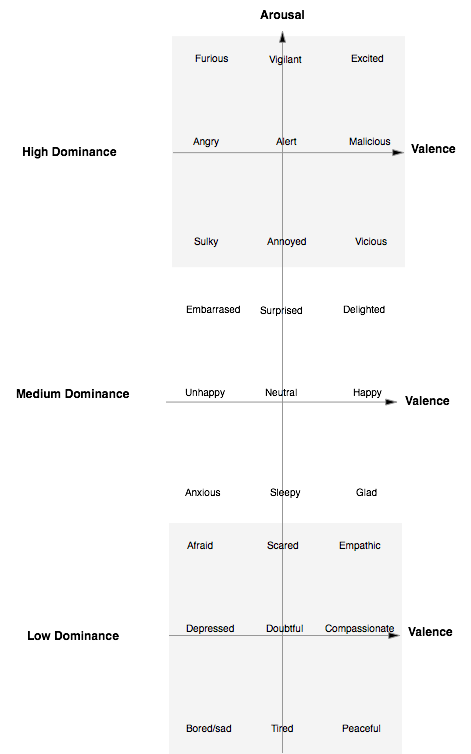
\includegraphics[height=5in]{VAD.png}}
  \centering
  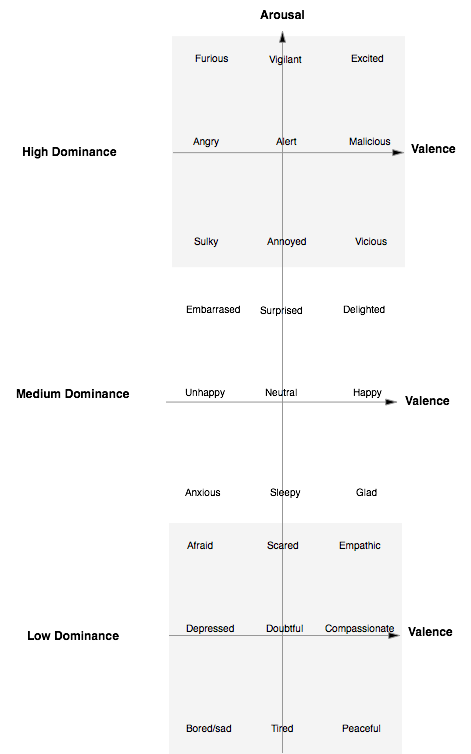
\includegraphics[height=0.6\textheight]{VAD.png}
\caption{VAD emotional values (figure adapted from~\citet{ahn2012nvc})} \label{fig:vad}
\end{figure}

In order to make the agents acting out the Punch and Judy show more believable,
we apply an emotional model to affect their actions and decisions. For this, we
use the valence-arousal (circumplex) model first described
by~\citet{russell1980circumplex}. To give each character its own distinct
personality, we extend this model with an extra dimension: dominance, as used
by~\citet{ahn2012nvc} in their model for conversational virtual humans. This
dominance level is affected by the reactions of the audience to the agents'
actions. For example, Judy may become more dominant as her suggestions to hit
Punch with a stick are cheered on by the audience, emboldening her into acting
out her impulses.

The VAD model, an extension of Russell's circumplex
model~\citep{russell1980circumplex}, illustrates how valence, arousal and
dominance values map to identifiable emotions. Valence, arousal and dominance
can each have a value of low, medium or high. This allows the agents to have a
total of 27 distinct emotional states, shown in Figure~\ref{fig:vad}.
The valence and arousal levels of each agent are affected by the actions of other agents. For example, a character being chased around the stage by Punch will see their valence level drop while their arousal increases. According to Russell's circumplex model of emotion~\citep{russell1980circumplex}, this would result in them becoming \emph{afraid\/} (if their dominance level is low).

An agent's emotional state affects its ability to fulfil its institutional obligations. An agent that is \emph{furious\/} might have no problem carrying out an obligation that requires them to kill another agent. If that same agent is \emph{happy\/} or \emph{depressed}, however, they might not have the appropriate motivation to perform such a violent action.

It is important to note that the emotional model is part of the agent belief state, and not held in the institution. We want to explore how the characters of the story might be able to choose actions based on their emotional state. While the institution could theoretically calculate the emotional state for each agent in turn and dictate this to them along with the norms of the narrative, it makes sense to decouple this feature from the narrative institution in order to separate the characters from the events of the story. %\jnote{review this paragraph}

Agents' emotional states change according to their interactions with the audience. This is unrelated to what is happening in the narrative, and so this underscores the decision not to include any emotional modelling in the institution. Also, we want the agents to have some degree of freedom within the narrative world. They should be allowed to determine their emotions themselves, so that in extreme emotional states they can perform `irrational' or `extreme' actions that may not necessarily fit into the narrative.

The actions of other agents in the simulation also affects characters' emotional
states. Section~\ref{sec:pj-fullspec} gives a further example of an agent emotional
model that take the actions of other agents into account.

\subsection{VAD emotions in Jason}
Emotions are implemented as beliefs inside an agent. An agent believes it has a certain level of valence, arousal and dominance, and it works out its emotional state based on a combination of these three factors. When the audience cheers or boos them, this changes the belief holding the relevant emotional variable, and their emotional state as a whole is recalculated.

Valence, arousal and dominance values can take values of -1 (low), 0 (medium) or 1 (high). Listing~\ref{lst:emotions} shows the emotional belief rules for an agent with medium dominance (a dominance level of 0). Note that an agent maintains beliefs about both its current emotion label (such as sleepy or happy) and the separate valence, arousal and dominance values at the same time.  Similar sets of rules handle the belief emotion for the other dominance levels.  %We address the matter of how external stimuli affect dominance in section~\ref{sec:norms as percepts}.\jnote{still needs doing}

Every time an emotional variable (valence, arousal, or dominance) changes, an agent's emotion is changed according to the rules in Listing~\ref{lst:emotions}. While an agent's valence, arousal and dominance belief values affect the way it makes decisions internally, the results of combinations of these values (sleepy, happy, etc) are broadcast as external actions. The reason for this is that an agent's emotional state may affect the way in which the character is animated: changing the speed at which they move or turning their smile into a frown, for example. For this reason, whenever an emotional change takes place, the new emotion is published as an external action of the agent so that observing entities may perceive it. The Bath sensor framework described in Section~\ref{sec:arch} provides the means for this evidence of the agent's internal state change to be received by the animation system and reflected accordingly in the display.

\begin{lstlisting}[float=!t,caption={Emotional rules for a character with medium dominance},label=lst:emotions,escapechar=\%,basicstyle=\scriptsize\ttfamily]
emotion(sleepy) :- valence(0) & arousal(-1) & dominance(0).
emotion(neutral) :- valence(0) & arousal(0) & dominance(0).
emotion(surprised) :- valence(0) & arousal(1) & dominance(0).
emotion(anxious) :- valence(-1) & arousal(-1) & dominance(0).
emotion(unhappy) :- valence(-1) & arousal(0) & dominance(0).
emotion(embarrassed) :- valence(-1) & arousal(1) & dominance(0).
emotion(glad) :- valence(1) & arousal(-1) & dominance(0).
emotion(happy) :- valence(1) & arousal(0) & dominance(0).
emotion(delighted) :- valence(1) & arousal(1) & dominance(0).
\end{lstlisting}

\begin{lstlisting}[float=!t,caption={AgentSpeak rules for changing an agent's
emotional values from audience
responses},label=lst:response,basicstyle=\scriptsize\ttfamily,escapechar=\%]
+!changeMood%\label{lne:changemood-start}%
  <- ?emotion(Z);
     emotion(Z).%\label{lne:changemood-end}%
+response(_, boo) : asking%\label{lne:response1-start}%
  <- -+valence(-1);
     -+dominance(-1);
     !changeMood.%\label{lne:response1-end}%
+response(_, cheer) : asking%\label{lne:response2-start}%
  <- -+valence(1);
     -+dominance(1);
     !changeMood.%\label{lne:response2-end}%
\end{lstlisting}

Listing~\ref{lst:response} shows the AgentSpeak rules describing how an agent's
valence and dominance levels are changed by the audience cheering or booing
their actions. These AgentSpeak plans describe what the agent should do in
response to a goal addition (denoted by a $\texttt{+!}$ at the start of the plan
name) or a belief addition (prefixed by a simple $\texttt{+}$). In the case of
Listing~\ref{lst:response}, the $\texttt{+!changeMood}$ plan on
lines~\ref{lne:changemood-start} to~\ref{lne:changemood-end} updates the agent's
emotional state based on its valence-arousal-dominance values and broadcasts the
result as an external action. The $\texttt{+response}$ plans
(Listing~\ref{lst:response}, lines~\ref{lne:response1-start} - \ref{lne:response1-end}
and~\ref{lne:response2-start} - \ref{lne:response2-end}) raise or lower an agent's valence and dominance levels depending on whether the agent perceives a ``boo'' or ``cheer'' response from the audience.

An agent announces what they intend to do, then waits three seconds. During this time, they have the belief that they are ``asking'' the audience, and listen for a response. A ``boo'' reduces an agent's valence and dominance, while a cheer raises them. For each response, the \texttt{changeMood} goal is triggered, which looks up and broadcasts the agent's emotional state to the other agents and environment.

\subsection{Agent decision making} \label{sec:decisions}
The agents choose which goals to pursue according to three factors: their permitted actions, their obliged actions and their emotional state. Though obliged actions are given priority, and while agents'' decisions are generally constrained by their permitted actions, an agent's emotional state has the final say in its decisions. In this way, an agent will follow the social norms of the narrative, but only according to their own mood.

\paragraph{Agent goals and plans}
% \subsection{Agent goals and plans}
The agents are implemented using a belief-desire-intention (BDI) psychological model using the Jason platform ~\citep{bordini2007programming}. An agent's knowledge about the state of their world and themselves are stored as \emph{beliefs}, with new information coming in from the environment getting added to their belief base as \emph{percepts}, which are ephemeral and only last for one reasoning cycle of an agent.

Agents are created with goals and plan libraries. Any goal that an agent is set on carrying out at any point is an \emph{intention}, whereas a goal that an agent has but is not yet pursuing is a \emph{desire}. Plan libraries describe the steps agents need to take in order to achieve goals, as well as how to react to changes in agents'' environments.

\paragraph{Norms as percepts}\label{sec:norms-as-percepts}
% \subsection{Norms as percepts}\label{sec:norms as percepts}
When an event occurs, it is added to the event timeline, which is used to query the ASP (Answer Set Programming) solver to obtain the set of norms that hold after the new event has occurred. The new permissions and obligations are then added to each agent as \emph{percepts}. Each time this happens, the set of permitted and obliged actions that an agent sees is changed to be only those that apply at that instant in time, with the previous norms being discarded.

Agents choose between permitted and obliged actions based on their emotional state at the point of decision making. Obliged actions are given a higher priority over permitted ones for most of the emotional states that an agent can be in, though not always. If an agent is in a sulky mood, for example, they may decide to ignore what they are obliged to do by the narrative, even though they know there will be consequences.

For example, in the scene where Joey gives the sausages to Punch, Punch may see that he has permission to eat the sausages, drop them, fight the crocodile, run away (leave the stage) or shout for help at the crocodile or audience. His obligation for the scene, in accordance with the Punch and Judy narrative world, is to either eat the sausages himself, or let the crocodile have them. This ends Propp's \emph{interdiction\/} story function with a \emph{violation\/} function. Note that his obligation in this case is not to guard the sausages as asked to by Joey. While Joey's entrusting of the sausages is certainly an obligation in itself, Punch's main obligations are to the narrative. Lesser obligations towards characters in the story can be implemented as having a lower prority than those of the story itself.

Similarly, at times of extreme emotion, an agent may decide to disregard their set of permitted actions entirely, instead acting out their innermost desires. For example, an angry Punch might decide to just attack Joey instead of agreeing to look after the sausages, or he might just decide to give up and leave if he is depressed. The key point is that the norms act as the will of the \emph{narrative}, guiding the story forward, rather than a strict set of rules that the agents must follow at all costs.

\emph{Violation events\/} add percepts to the agents telling them that they are in violation of the narrative norms. Once an agent receives such a percept, an emotional variable is changed. Typically, their dominance will decrease. The reasoning behind this is that if agents are unwilling to participate in the story, they should have less influence in its course of events.

\subsection{Architecture}\label{sec:arch}

\paragraph{Multi-Agent System:} \label{sec:arch-mas}
% \subsection{Multi-Agent System} \label{sec:inst}
We use the Jason~\citep{bordini2007programming} framework for belief-desire-intention (BDI) agents, with a VAD
emotional model as described above.

\paragraph{Institutional Framework}
% \subsection{Institutional Framework}
% How you used instAL to model Propp
To describe our institutional model, we use InstAL~\citep{cliffe2007specifying}, a domain-specific (action) language for describing institutions that compiles to AnsProlog, a declarative programming language for Answer Set Programming (ASP). InstAL's semantics are inspired by the Situation Calculus~\citep{reiter1991frame} and the Event Calculus~\citep{kowalski1989logic}. InstAL describes how external events generate institutional events, which then initiate or terminate fluents that hold at certain points in time. These fluents can include the permissions and obligations that describe what an agent is permitted or obliged to do when, as described in Section~\ref{sec:pjexample-insts}.
For example, if an agent with the role of \emph{dispatcher\/} leaves the stage,
it generates the Propp \emph{absentation\/} move in the institution, but only if
the \emph{interdiction} function is active (i.e., the
\emph{activeFunction(interdiction)} fluent holds): %\mnote{Added \emph{activeFunction} explanation}
\begin{lstlisting}[basicstyle=\scriptsize\ttfamily]
leaveStage(X) generates intAbsentation(X)
   if role(X, dispatcher), activeFunction(interdiction);
\end{lstlisting}
% \vspace{-1cm}
which generates the following AnsProlog code:\\
\begin{minipage}{0.6\textwidth}
\begin{lstlisting}[basicstyle=\scriptsize\ttfamily,escapechar=\%]
occurred(intAbsentation(X),pj,I) :-%\mylabel{t1}%
   occurred(leaveStage(X),pj,I),%\mylabel{t2}%
   holdsat(pow(pj,intAbsentation(X)),pj,I),%\mylabel{t3}%
   holdsat(role(X,donor),pj,I),%\mylabel{t4}%
   holdsat(activeFunction(interdiction),pj,I), %\mylabel{t5}%
   agent(X), inst(pj), instant(I).%\mylabel{t6}%
\end{lstlisting}
\end{minipage}\hspace{0.08\textwidth}%\hfill
\begin{minipage}{0.3\textwidth}\scriptsize
\myref{t1}{s1}{The internal \emph{absentation} event occurs if the following conditions are met:}
\myref{t2}{s2}{$\bullet X$ leaves the stage}
\myref{t3}{s3}{$\bullet X$ has the power to leave the stage}
\myref{t4}{s4}{$\bullet X$ has the role of donor}
\myref{t5}{s5}{$\bullet$ the \emph{interdiction} function is active}
\myref{t6}{s6}{$\bullet X$ is an agent, pj is an institution, $I$ is an instant}
\end{minipage}\\
The \emph{absentation\/} institutional event gives the crocodile permission to enter the stage if there are any sausages on the stage. It also terminates the permission of the absented agent to leave the stage, as they have already done so:\\
\begin{minipage}{0.6\textwidth}
\begin{lstlisting}[basicstyle=\scriptsize\ttfamily,escapechar=\%]
intAbsentation(X) initiates perm(enterStage(croc)) if objStage(sausages);%\mylabel{t1}%
intAbsentation(X) terminates onStage(X), perm(leaveStage(X));%\mylabel{t2}%
\end{lstlisting}
\end{minipage}\hspace{0.08\textwidth}%\hfill
\begin{minipage}{0.3\textwidth}\scriptsize
  \myref{t1}{s1}{The \emph{absentation} function gives the crocodile permission to enter the stage if the sausages are on stage}
  \myref{t2}{s2}{The \emph{absentation} function means that once X leaves the stage, they are no longer on stage}
\end{minipage}\\
which generates the following:\\
\begin{minipage}{0.6\textwidth}
\begin{lstlisting}[basicstyle=\scriptsize\ttfamily,escapechar=\%]
initiated(perm(enterStage(croc)),pj,I) :-%\mylabel{t1}%
   occurred(intAbsentation(X),pj,I),%\mylabel{t2}%
   holdsat(live(pj),pj,I), inst(pj),%\mylabel{t3}%
   holdsat(objStage(sausages),pj,I),%\mylabel{t4}%
   agent(X), inst(pj), instant(I).%\mylabel{t5}%
\end{lstlisting}
\end{minipage}\hspace{0.08\textwidth}%\hfill
\begin{minipage}{0.3\textwidth}\scriptsize
\myref{t1}{s1}{The crocodile gets permission to enter the stage if the following
  conditions are met:}
\myref{t2}{s2}{$\bullet$ the \emph{absentation} function event has occured}
\myref{t3}{s3}{$\bullet$ the pj institution is running}
\myref{t4}{s4}{$\bullet$ the sausages are on stage}
% \myref{t5}{s5}{$\bullet X$ is an agent, pj is an institution, $I$ is an instant}
\end{minipage}\\
%% \begin{comment}
%% If the ``defeat'' institutional event occurs (as a result of a struggle between
%% two agents), it initiates a fluent signifying that that agent is dead, along
%% with an obligation for the agent to leave the stage. If they don't leave the
%% stage, then they are in violation of the scene, and an appropriate violation
%% event is triggered. Also note that the fluent and obligation event are only
%% initiated \emph{if} the agent is playing the role of a victim:
%% \begin{lstlisting}[basicstyle=\scriptsize\ttfamily]
%% intDefeat(X, Y) initiates dead(Y), obl(leaveStage(Y), deadline, vioScene(Y)) if role(Y, victim);
%% \end{lstlisting}
%% \end{comment}
\begin{figure}[!t]
\begin{minipage}{0.6\textwidth}
\begin{lstlisting}[caption={Encoding of Propp's \emph{absentation\/} function},basicstyle=\scriptsize\ttfamily,label=lst:absentation,escapechar=\%]
intAbsentation(X) initiates activeFunction(absentation);%\mylabel{t0}%
intAbsentation(X) initiates perm(harm(Y, Z)) if role(Y, villain), objStage(Z), onStage(Y), activeFunction(interdiction);%\mylabel{t1}%
intAbsentation(X) initiates perm(harm(Y, Z)) if role(Y, ambusher), objStage(Z), onStage(Y), activeFunction(interdiction);%\mylabel{t2}%
intAbsentation(X) initiates perm(enterStage(X)), activeFunction(absentation);%\mylabel{t3}%
intAbsentation(X) initiates perm(enterStage(croc)) if objStage(sausages);%\mylabel{t4}% 
intAbsentation(X) terminates onStage(X), perm(leaveStage(X));%\mylabel{t5}%
\end{lstlisting}
\end{minipage}\hspace{0.08\textwidth}%\hfill
\begin{minipage}{0.3\textwidth}\scriptsize
  \myref{t0}{s0}{The \emph{activeFunction(absentation)} function holds after any
    \emph{intAbsentation} institutional event, indicating that that Propp
    function is currently underway}
  \myref{t1}{s1}{The \emph{absentation} function gives the villain permission to harm
    an object, if both are on stage and the \emph{interdiction} function is active}
  \myref{t2}{s2}{Same as above, but for \emph{ambusher} role}
  \myref{t3}{s3}{The absented character has permission the re-enter the stage at any point during the \emph{absentation} function}
  \myref{t4}{s4}{The crocodile has permission to enter the stage if the sausages are on stage}
  \myref{t5}{s5}{The \emph{absentation} function means that the absented character is no longer on stage, and cannot leave the stage (as they have already done so)}
\end{minipage}
\end{figure}
By combining statements such as the above, we can build a complete description
of the sausages scene in terms of agent norms, such as the Propp
\emph{absentation} function, shown in Listing~\ref{lst:absentation}. InstAL rules like those shown above and in Listing~\ref{lst:absentation} are compiled into AnsProlog, then we use the \emph{clingo} answer set solver~\citep{gebser2011potassco} to ground the program, and `solve' queries by finding all permissions and obligations that apply to any agents, given a sequence of events as the query input. The agents' percepts are then updated with their permitted and obliged actions from that time instant onwards.  Thus, the institutional model acts as a social narrative sensor, interpreting actors' actions in the context of the combination of the concrete narrative and the abstract story moves which detach (instantiate) the norms that guide the actors in the direction of the conclusion of the story arc.

A query is simply a list of external events in chronological order, also called
a \emph{trace}. A possible trace describing the actions of agents acting out the
\emph{sausages} is described in Listing~\ref{lst:trace}. The `pj' in the trace
is the name of the institution that observes the events, while the
number is the enumeration of events in the sequence.

\begin{figure}[!t]
\begin{minipage}{0.6\textwidth}
% \newsavebox{\lstasp}
% \begin{lrbox}{\lstasp}
\begin{lstlisting}[caption={Possible full trace for sausages scene},label=lst:trace,basicstyle=\scriptsize\ttfamily,escapechar=\%]
observed(startShow,pj,0). %\mylabel{t1}%
observed(startScene(sausages),pj,1). %\mylabel{t2}%
observed(enterStage(punch),pj,2). %\mylabel{t3}%
observed(enterStage(joey),pj,3). %\mylabel{t4}%
observed(say(joey, give),pj,4). %\mylabel{t5}%
observed(say(joey,  protect),pj,5). %\mylabel{t6}%
observed(give(joey,punch,sausages),pj,6). %\mylabel{t7}%
observed(leaveStage(joey),pj,7). %\mylabel{t8}%
observed(say(punch, harm),pj,8). %\mylabel{t9}%
observed(enterStage(croc),pj,9). %\mylabel{t10}%
observed(take(croc, sausages),pj,10). %\mylabel{t11}%
observed(eat(croc, sausages),pj,11). %\mylabel{t12}%
observed(leaveStage(croc),pj,12). %\mylabel{t13}%
observed(enterStage(joey),pj,13). %\mylabel{t14}%
observed(hit(joey, punch),pj,14). %\mylabel{t15}%
observed(leaveStage(joey),pj,15). %\mylabel{t16}%
observed(leaveStage(punch),pj,16). %\mylabel{t17}%
observed(startScene(end),pj,17). %\mylabel{t18}%
\end{lstlisting}
\end{minipage}\hspace{0.08\textwidth}%\hfill
\begin{minipage}{0.3\textwidth}\scriptsize
  \myref{t1}{s1}{The show has started}
  \myref{t2}{s2}{The sausages scene has started}
  \myref{t3}{s3}{Punch has entered the stage}
  \myref{t4}{s4}{Joey has entered the stage}
  \myref{t5}{s5}{Joey says he will give Punch the sausages}
  \myref{t6}{s6}{Joey tells Punch to protect the sausages}
  \myref{t7}{s7}{Joey gives the sausages to Punch}
  \myref{t8}{s8}{Joey leaves the stage}
  \myref{t9}{s9}{Punch says he will eat the sausages}
  \myref{t10}{s10}{The crocodile enters the stage}
  \myref{t11}{s11}{The crocodile takes the sausages}
  \myref{t12}{s12}{The crocodile eats the sausages}
  \myref{t13}{s13}{The crocodile leaves the stage}
  \myref{t14}{s14}{Joey enters the stage}
  \myref{t15}{s15}{Joey hits Punch}
  \myref{t16}{s16}{Joey leaves the stage}
  \myref{t17}{s17}{Punch leaves the stage}
  \myref{t18}{s18}{The scene ends}
\end{minipage}
\end{figure}

Each \emph{observed} event triggers a corresponding \emph{occurs} event inside the
institution, as determined by the generates relation. Listing~\ref{lst:asp}
shows an extract from an answer set output for the trace queried against the ASP
description of the sausages scenario, for events~5 to~7 of the scene. Starting with an initial set of fluents that hold at instant~5,
only fluents that have been initiated and not terminated hold at the next
instant. For ease of reading, the listing only shows roles that hold at
certain instants when they have some effect on the scene, although in practice, all role fluents hold throughout the scene. Figure~\ref{fig:tracevis} shows a visualisation of the answer set for the trace in Listing~\ref{lst:trace}.

\begin{figure}[!t]
\begin{minipage}{0.65\textwidth}
%% \newsavebox{\lstasp}
%% \begin{lrbox}{\lstasp}
\begin{lstlisting}[caption={Sausages scene using ASP},label=lst:asp,basicstyle=\scriptsize\ttfamily,label=lst:asp,escapechar=\%]
holdsat(perm(say(donor, protect),pj,5).%\mylabel{t1}%
holdsat(role(joey, donor),pj,5).%\mylabel{t2}%
occurred(say(joey, protect),pj,5).%\mylabel{t3}%

initiated(activeFunction(interdiction),pj,6).%\mylabel{t4}%
initiated(perm(give(donor, villain, object)),pj,6).%\mylabel{t5}%
terminated(perm(say(donor, protect)),pj,6).%\mylabel{t6}%
holdsat(perm(give(donor, villain, object)),pj,6).%\mylabel{t7}%
holdsat(activeFunction(interdiction),pj,6).%\mylabel{t8}%
holdsat(role(joey, donor),pj,6).%\mylabel{t9}%
holdsat(role(punch, villain),pj,6).%\mylabel{t10}%
holdsat(object(sausages),pj,6).%\mylabel{t11}%
occurred(give(joey, punch, sausages),pj,6).%\mylabel{t12}%

initiated(activeFunction(absentation),pj,7).%\mylabel{t13}%
initiated(perm(leavestage(donor)),pj,7).%\mylabel{t14}%
terminated(perm(give(donor, villain, object)),pj,7).%\mylabel{t15}%
holdsat(activeFunction(interdiction),pj,7).%\mylabel{t16}%
holdsat(activeFunction(absentation),pj,7).%\mylabel{t17}%
holdsat(role(joey, donor),pj,7).%\mylabel{t18}%
holdsat(perm(leavestage(donor)),pj,7).%\mylabel{t19}%
\end{lstlisting}
\end{minipage}\hspace{0.03\textwidth}%\hfill
% \end{lrbox}
% \noindent\usebox{\lstasp}\hfill
\begin{minipage}{0.3\textwidth}\scriptsize
  \myref{t1}{s1}{The donor role can tell someone to protect an object at instant 5}
  \myref{t2}{s2}{Joey is the donor at instant 5}
  \myref{t3}{s3}{Joey tells another character to protect an object at instant 5}
  \myref{t4}{s4}{The \emph{interdiction} function becomes active at instant 6}
  \myref{t5}{s5}{The donor has permission to give an object to the villain at instant 6}
  \myref{t6}{s6}{The donor can no longer tell anyone to protect an object at instant 6}
  \myref{t7}{s7}{The donor can give an object to the villain at instant 6}
  \myref{t8}{s8}{The \emph{interdiction} function is active at instant 6}
  \myref{t9}{s9}{Joey is the donor at instant 6}
  \myref{t10}{s10}{Punch is the villain at instant 6}
  \myref{t11}{s11}{Sausages are an object at instant 6}
  \myref{t12}{s12}{Joey gives the sausages to Punch at instant 6}
  \myref{t13}{s13}{The \emph{absentation} function becomes active at instant 7}
  \myref{t14}{s14}{The donor can leave the stage at instant 7}
  \myref{t15}{s15}{The donor can give an object to the villain at instant 7}
  \myref{t16}{s16}{The \emph{interdiction} function is active at instant 7}
  \myref{t17}{s17}{The \emph{absentation} function is active at instant 7}
  \myref{t18}{s18}{Joey is the donor at instant 7}
  \myref{t19}{s19}{The donor can leave the stage at instant 7}
\end{minipage}
\end{figure}

% \begin{figure}[!t]
% 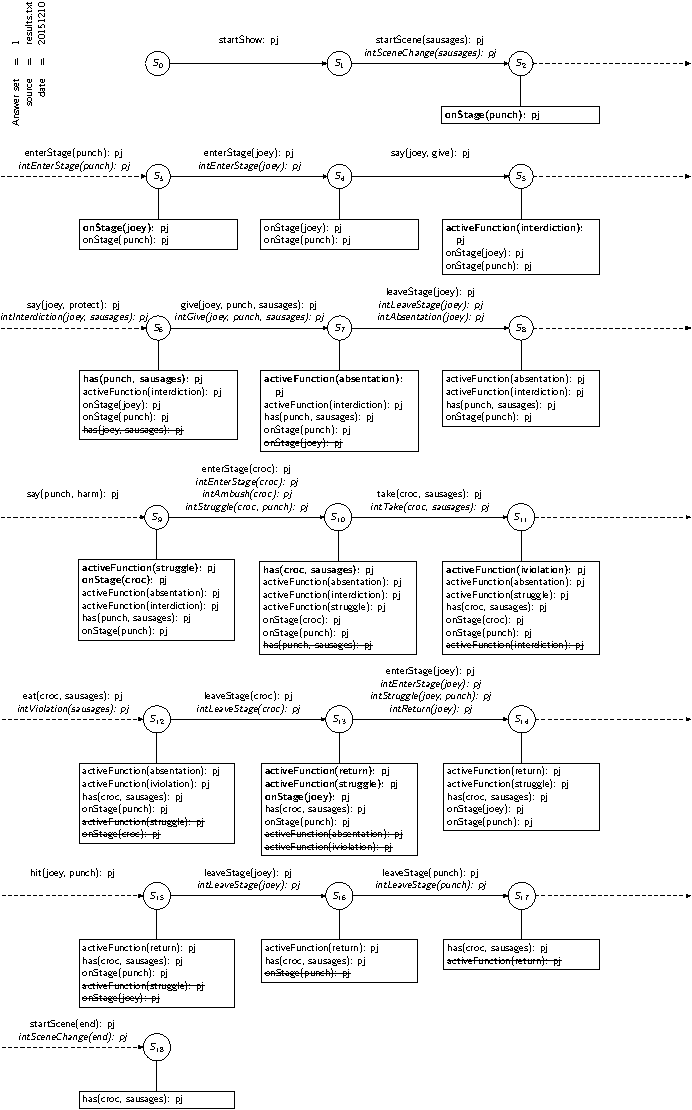
\includegraphics[width=1.3\linewidth]{trace.pdf}
% \caption{Visualised trace of the sausages scene} \label{fig:vis}
% \end{figure}

\begin{figure}[!p]
%     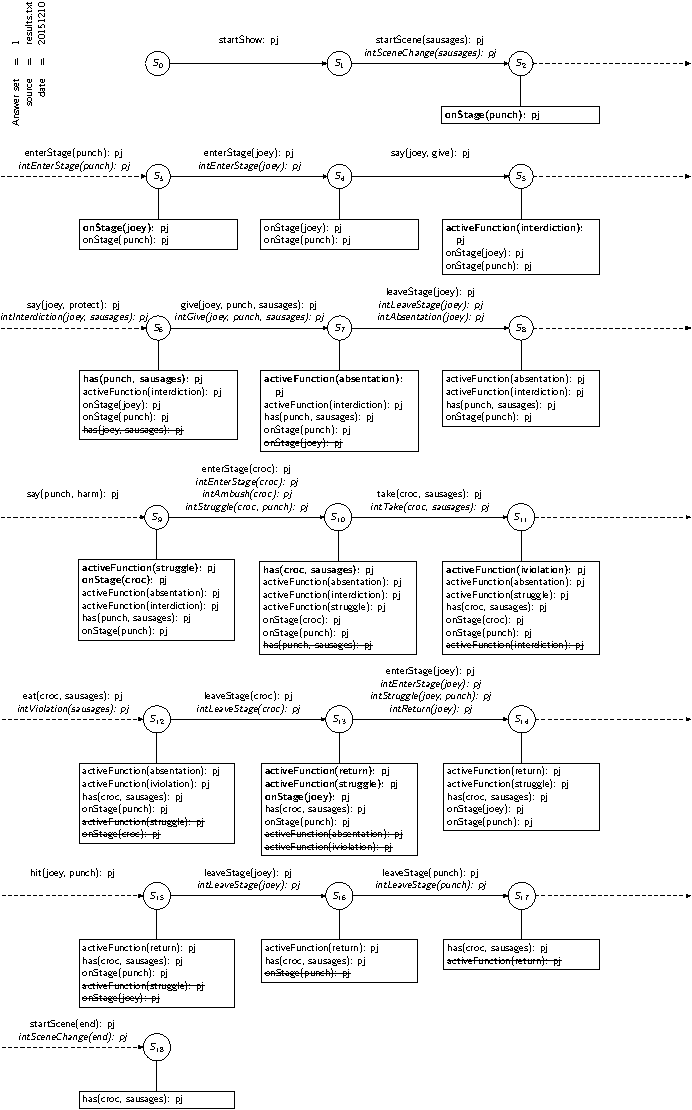
\includegraphics[width=\linewidth]{trace.pdf}
    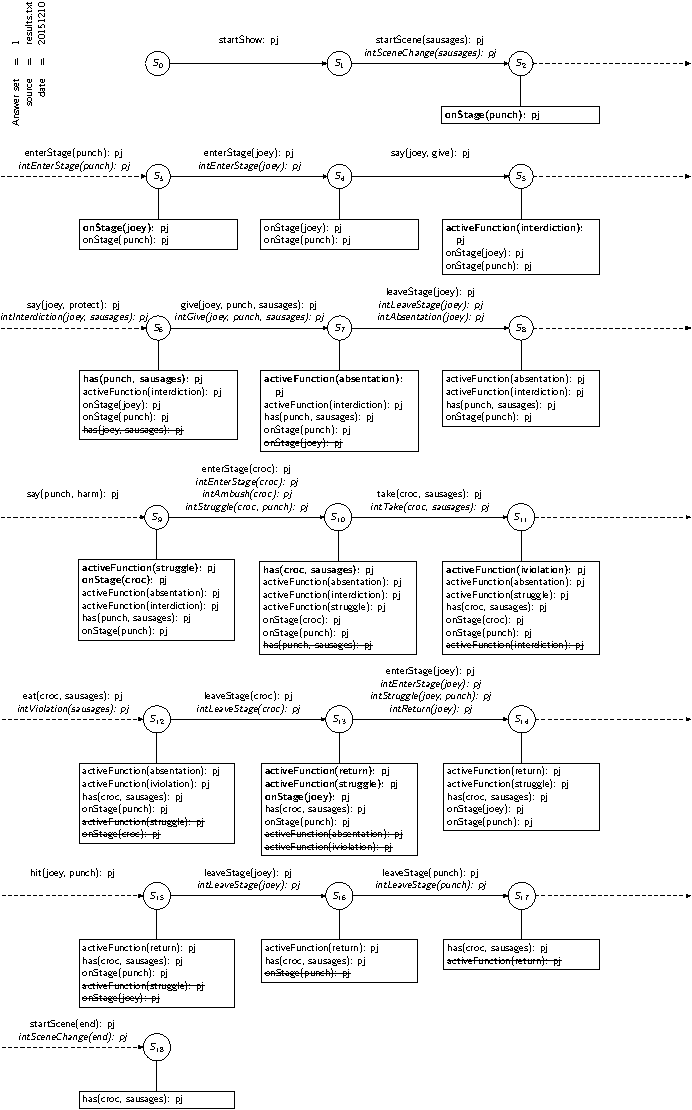
\includegraphics[height=0.95\textheight]{trace.pdf}
    \caption{Trace visualisation} \label{fig:tracevis}
\end{figure}

% 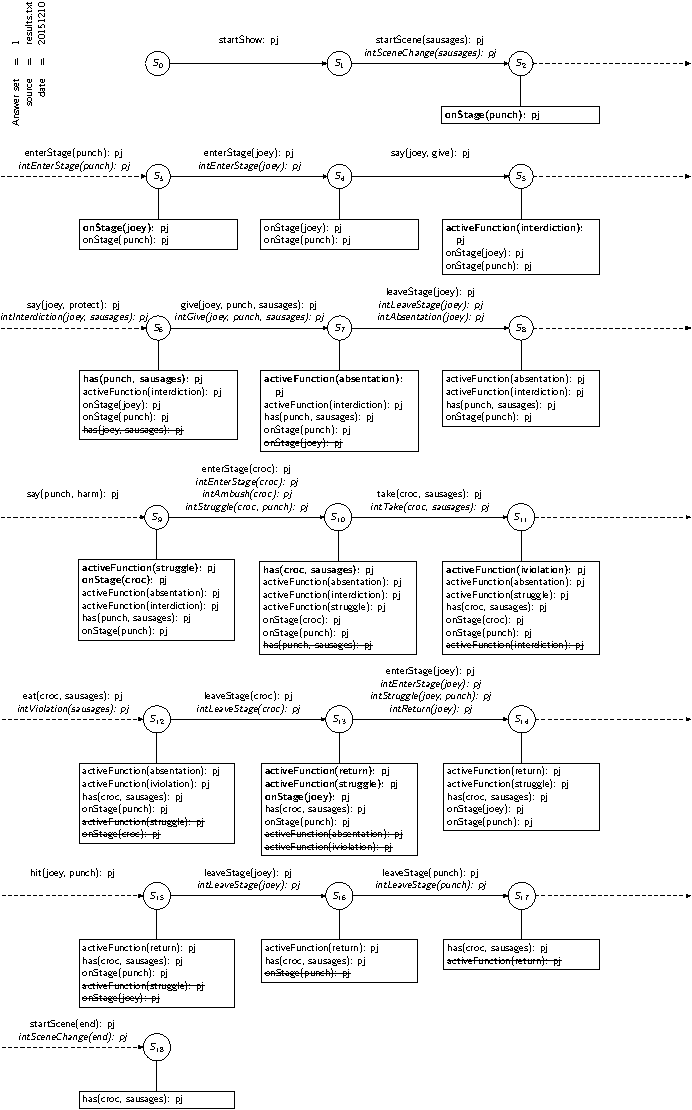
\includepdf{trace.pdf}

%\lstinputlisting[language=prolog, firstline=74, lastline=74]{pj_model.ial}

%\begin{lstlisting}[language=prolog, frame=single]  % Start your code-block
%enterStage(X) generates intReturn(X, Z) if role(X, dispatcher), role(Y, villain), onStage(Y);
%\end{lstlisting}

\begin{figure}[!t]
% \includegraphics[height=3in]{arch1.png}
% \begin{minipage}{0.58\textwidth}
% \includegraphics[width=\textwidth]{arch1.png}
% \end{minipage}\hfill
% \begin{minipage}{0.38\textwidth}\raggedright
% \end{minipage}
% \caption{System architecture} \label{fig:arch}
% % \end{figure}
% % \begin{figure}[!t]
% \medskip
\begin{minipage}{0.56\textwidth}
\includegraphics[width=\textwidth]{punchjudy.png}
\end{minipage}\hfill%
% \includegraphics[height=2in]{punchjudy.png}
\begin{minipage}{0.4\textwidth}
% The animation engine that shows the visual output of the agents actions is written in Javascript and the Phaser game framework. It runs entirely in a browser, and communicates with BSF using the Strophe XMPP library.
The animation engine that shows the visual output of the agents actions is written in Javascript and the Phaser game framework. It runs entirely in a browser, and communicates with BSF using the Strophe XMPP library.

If the user allows the program access to their microphone, they can cheer or boo the actions of the agents by shouting into the microphone. Otherwise, they can simulate these actions by clicking on `cheer' or `boo' buttons at the bottom of the screen.
\end{minipage}
\caption{A screenshot of the Punch and Judy show} \label{fig:pjshow}
\end{figure}

\paragraph{Bath Sensor Framework} The components communicate using the Bath Sensor Framework
(BSF)~\citep{lee2013decoupling}, through publish / subscribe-style communication between distributed software components, in this case connecting intelligent agents with their virtual environments. It currently uses the XMPP publish/subscribe protocol for communication between agents, environment and other software components. Each agent subscribes to receive notifications of environment changes via the appropriate topic node in the XMPP server, which relays messages between publishers and subscribers. If any environment change occurs, all subscribed agents are informed of the changes.

\paragraph{Audience Interaction} \label{sec:demo}
% Explain what will happen
The puppet show is designed to be run in front of either a single user's computer, or on a large display in front of an audience. The user/audience is instructed to cheer or boo the actions of the characters of the show, which will be picked up by a microphone and `heard' by the agents. This will then affect the emotional state of the agents and change the actions they make in the show. Their actions are constrained by the set of `Punch and Judy' world norms as described in the institutional model.

There are many different ways in which the audience's responses can affect the outcomes of the show. If the audience craves a more `traditional' Punch and Judy experience, then they can cheer Punch into beating and killing all of his adversaries (including his wife, Judy). Alternatively, a more mischievous audience could goad Judy into killing Punch and then taking over his role as sadist and killer for the rest of the show. The narrative outcomes are dependent on how the audience responds to the action, yet still conform to the rules of the Punch and Judy story world.

\section{Summary}
\label{sec:inst-summary}
Our implementation of the interactive Punch and Judy show demonstrates several
advantages in using social institutions to model narrative. Addressing the issue
of limited agent autonomy in existing systems (Issue~\ref{iss:freedom} from
Section~\ref{sec:litrev-discussion}), the advantages of this approach are:

\begin{itemize}
  \item Because norms encourage rather than enforce actions, agents are give
    more flexibility in their behaviour. While their actions are encouraged to
    conform to a narrative for the most part, an author could insert mechanisms
    by which agents are able to ``break away'' from the confines of the story.
    For example, if each agent were to have an emotional model, they could carry
    out story-disrupting actions in times of extreme emotional distress.
  \item Rather than thinking about and describing the goals of a story (as with
    a planner-based system), a narrative is described in terms of what
    \emph{may} and \emph{must} happen. This gives an author more control over
    the flexibility of their stories, as they can describe optional paths
    through a story rather than setting hards goals that must always be
    satisfied.
  \item Through the use of InstAL and its compilation to ASP, we can generate
    all of the possible actions in each story path as answer sets.
\end{itemize}

A major shortcoming describing stories in terms of
institutions is the learning effort it requires from a non-programmer (such as a
story author). An author would need to fully understand a narrative formalism (such as Propp's \emph{Morphology} from this chapter's
example) in order to describe their story using logical components. Our aim is
to allow authors to describe their stories without the burden of learning that
comes with current approaches. For this reason, Chapter~\ref{cha:tropes} explains how
\emph{story tropes} may be used by authors to describe parts of a story
without the need to learn the rules of a narrative formalism such as Propp's.
These tropes are used to develop \emph{TropICAL}, our controlled
natural-language system for defining story components, which we describe in Chapter~\ref{cha:tropical}.

\chapter{Evaluation \& Validation}
\label{cha:evaluation}
\added{

}{New chapter for Evaluation and Validation}
\section{A Full Specification of Punch and Judy}
\label{sec:pj-fullspec}
In section~\ref{sec:punchjudy-tropes}, we describe one scene from Punch and Judy
in terms of tropes. The scene chosen in this example is one where a crocodile
appears on stage to steal some sausages that Punch is guarding. This section
gives an example of a \emph{full} Punch and Judy show described in terms of
tropes, including the ``sausages'' scene described previously.

Though each retelling of the Punch and Judy story may use a different number of
scenes in varying order, we use the following scenes for our ``minimal'' Punch
and Judy example:

\begin{itemize}
\item \textbf{Introduction}: Joey the clown introduces the show and interacts
  with the audience
\item \textbf{Punch, Judy and the Baby}: Judy asks Punch to look after the baby,
  which he then kills. Punch then also kills Judy.
\item \textbf{Punch and the Policeman}: A policeman comes to arrest Punch, and
  is killed.
\item \textbf{Crocodile and Sausages Scene}: Joey asks Punch to look after some
  sausages, which are then eaten by a crocodile.
\item \textbf{Punch and the Devil}: Punch fights the Devil, killing him.
\end{itemize}

\subsection{``Introduction'' Scene}
\label{sec:full-introduction}
% Tropes: audience participation, narrator, exposition?, exposition?
In the \emph{introduction} scene of Punch and Judy, Joey the Clown appears on stage to
introduce the show to the audience. During the scene, Joey provokes an audience
response by asking the audience to, for example, summon the Punch and Judy
characters from backstage.

The tropes that appear in this scene would be:

\begin{itemize}
\item \textbf{Narrator}: Joey the Clown appears to be a narrator of sorts, who
introduces the show. Due to his narrator status, he appears to be immune from
Punch's attacks.
\item \textbf{Audience Participation}: Joey asks the audience to call out certain
phrases during the introduction, often getting them to repeat themselves by
calling out ``Louder! I can't hear you!'', for example.
\end{itemize}

The essence of the ``Narrator'' trope is simply to have a character that is able
to talk to the audience. Listing~\ref{lst:pjfull-narrator} shows how this trope
would be described in TropICAL.

\begin{lstlisting}[showstringspaces=false, label={lst:pjfull-narrator}, caption={The ``Narrator'' trope}]
"Narrator" is a trope where:
  The Narrator is a role
  The Audience is a role
  The Narrator talks to the Audience
\end{lstlisting}

In the ``Audience Participation'' trope, characters can talk to the audience,
and the audience is also able to talk back.
Listing~\ref{lst:pjfull-participation} shows how this trope could be translated
to TropICAL. In this example, certain characters can be assigned the role of
``Audience-aware character''. Any character with this role would be able to talk
to the audience, and the audience would be able to talk back to them.

\begin{lstlisting}[showstringspaces=false, label={lst:pjfull-participation}, caption={The ``Audience Participation'' trope}]
"Audience Participation" is a trope where:
  Audience-Aware Character is a role
  The Audience is a role
  The Audience-Aware Character talks to the Audience
  Then the Audience talks to the Audience-Aware Character
\end{lstlisting}

\subsection{``Punch, Judy and the Baby'' Scene}
% Tropes: don't touch it, you idiot, put on a bus, chase fight, the bus came back
% We can make this into an abstraction, as it's also featured in the sausages scene
% Call the new trope: set the scene for mischief
% May want to possibly add parental abandonment as well

In this scene, Punch and Judy appear on stage. After some comic dialogue, Judy
announces that she needs to leave the stage, leaving Punch to take care of their
baby. Punch chases the baby around the stage, finally hitting it with his stick,
knocking it off stage and killing it. Judy returns to find that the baby is
missing, and Punch and Judy have an argue. The argument ends with Punch hitting
his wife with a stick, killing her.

This scene contains the following tropes:

\begin{itemize}
\item \textbf{Audience Participation}: as defined above
\item \textbf{Don't touch it, you idiot!}: as defined earlier in
Section~\ref{sec:dont-touch-inst}, this is where Judy tells Punch to look after
the baby.
\item \textbf{Put on a bus / the bus came back}: Judy then leaves the stage, only to
come back later to discover that Punch has killed the baby
\item \textbf{Chase fight}: Punch chases Judy around the stage with a stick
\item \textbf{Domestic Abuse}: Punch beats and kills Judy
\end{itemize}

We define the TropICAL translation of the audience participation trope in the
previous section (Section~\ref{sec:full-introduction}).

The combination of ``Don't Touch It, You Idiot!'' and ``Put On a Bus / The Bus
Came Back'' is a common occurrence in Punch and Judy - it also appears in the
``Sausages and Crocodile'' scene. For this reason, it makes sense to create a new
trope which is a hybrid of the two. We call this trope ``Setting the Scene for
Mischief'', and its TropICAL interpretation appears in Listing~\ref{lst:pjfull-mischief}

\begin{lstlisting}[showstringspaces=false, label={lst:pjfull-mischief}, caption={The ``Setting the Scene
For Mischief'' trope}]
"Setting the Scene for Mischief" is a trope where:
  The Owner is a role
  The Idiot is a role
  The Item is an object
  Away is a place
  The Owner entrusts the Idiot with the Item
  Then the Owner goes Away
  Then the Idiot breaks the Item
  Then the Owner returns
  Then the Owner fights the Idiot
\end{lstlisting}

\begin{lstlisting}[showstringspaces=false, label={lst:pjfull-chasefight}, caption={The ``Chase
Fight'' trope}]
"Chase Fight" is a trope where:
  The Pursuer is a role
  The Pursuee is a role
  The Pursuer chases the Pursuee
  Then the Pursuee fights the Pursuer
  Then the Pursuer kills the Pursuee
    Or the Pursuee escapes
\end{lstlisting}

The ``Domestic Abuse'' trope simply describes a situation in which a husband and
wife fight with each other, as described in the TropICAL code in Listing~\ref{lst:pjfull-domesticabuse}.

\begin{lstlisting}[showstringspaces=false, label={lst:pjfull-domesticabuse}, caption={The ``Domestic
Abuse'' trope}]
"Domestic Abuse" is a trope where:
  The Wife is a role
  The Husband is a role
  The Wife fights the Husband
    Or the Husband fights the Wife
\end{lstlisting}

\subsection{``Punch and the Policeman'' Scene}
% Tropes: slapstick, amusing injuries, chase fight, mini-boss
% Abstracted to: slapstick confrontation

In this scene, Punch is confronted by the Policeman character, who attempts to
arrest him for the murder of his wife and baby. Punch chases the Policeman
around the stage, hitting him with a stick and finally murdering him as well.

This scene contains the following tropes:

\begin{itemize}
\item \textbf{Slapstick}: the characters hit each other in a comedic way
\item \textbf{Chase Fight}: one character chases another and fights them, as defined above
\item \textbf{Mini-boss}: the protagonist must defeat an enemy to continue the quest
\end{itemize}

The slapstick trope can be defined in TropICAL with the code shown in Listing~\ref{lst:pjfull-slapstick}.

\begin{lstlisting}[showstringspaces=false, label={lst:pjfull-slapstick}, caption={The ``Slapstick'' trope}]
"Slapstick" is a trope where:
  The Slapper is a role
  The Slapped is a role
  The Slapper slaps the Slapped
  Then the Slapped slaps the Slapper
\end{lstlisting}

The ``Chase Fight'' trope already appears in the previous scene where Punch kills his baby and wife (Listing~\ref{lst:pjfull-chasefight}), 
so we can re-use that trope for this scene.

\begin{lstlisting}[showstringspaces=false, label=lst:pjfull-miniboss,caption={The
``Mini-boss'' trope in TropICAL}]
"Mini-boss" is a trope where:
  The Hero is a role
  The Mini-Boss is a role
  The Hero fights the Mini-Boss
  Then the Hero defeats the Mini-Boss
    Or the Hero dies
      Then the story ends
  Then the Hero escapes
\end{lstlisting}

The translation of the ``Mini-boss'' trope into TropICAL code is shown in Listing~\ref{lst:pjfull-miniboss}.

\subsection{``Crocodile and Sausages'' Scene}
% Tropes: set the scene for mischief (see above)
\label{sec:croc-sausages-scene}

This scene can simply re-use the ``Setting the Scene for Mischief'' trope from
the previous scene with Punch, Judy and the baby. In this case, Joey the Clown
takes the place of Judy as the ``Owner'', telling him to look after an ``Item''.
In this case, the item takes the form of some sausages instead of a baby.

The only difference here is that instead of the ``Idiot'' breaking the item, it
is broken by the ``Crocodile''. This means that in order to use the ``Setting
the Scene for Mischief'' trope, we need to modify it so that the ``Mischief''
that occurs can include events other than the ``Idiot'' breaking an item.
Listing~\ref{lst:pjfull-mishandling} shows a trope named ``Mishandling of an Item'' that describes the various
ways in which an item can be mishandled. Listing~\ref{lst:pjfull-mischief2} is
the redefined ``Setting the Scene for Mischief'' trope, with the replacement of
the Idiot breaking the Item with the ``Mishandling of an Item'' trope.

\begin{lstlisting}[showstringspaces=false,
label=lst:pjfull-mishandling,caption={The ``Mishandling of an Item'' trope in TropICAL}]
"Mishandling of an Item" is a trope where:
  The Idiot is a role
  The Accomplice is a role
  The Item is an object
  Onstage is a place
  The Idiot breaks the Item
    Or the Idiot loses the Item
    Or the Accomplice goes Onstage
      Then the Accomplice breaks the Item
        Or the Accomplice loses the Item
\end{lstlisting}

\begin{lstlisting}[showstringspaces=false,
label=lst:pjfull-mischief2,caption={The ``Setting the Scene for Mischief''
trope with ``Mishandling of an Item'' embedded}]
"Setting the Scene for Mischief" is a trope where:
  The Owner is a role
  The Idiot is a role
  The Item is an object
  Away is a place
  Home is a place
  The Owner tells the Idiot to protect the Item
  Then the Owner goes Away
  Then the "Mishandling of an Item" trope happens
  Then the Owner returns Home
  Then the Owner fights the Idiot
\end{lstlisting}


\subsection{``Punch and the Devil'' Scene}
% Tropes: slapstick confrontation (can we change mini-boss to boss?)
This scene often (but not always) closes the Punch and Judy show. In it, the
Devil himself confronts Punch. Punch, however, is not intimidated, and he chases
the Devil around the stage before beating him to death with his stick.

This scene plays out in exactly the same way as the ``Punch and the Policeman''
scene, so we can re-use the same tropes: \textbf{Slapstick}, \textbf{Chase
  Fight} and \textbf{Mini-Boss}.

\subsection{Putting It All Together}
\label{sec:put-together-pj}
% Look at chaining the above together, and adding meta-tropes that are present throughout (such as audience participation, which you should discuss before)
Having defined the tropes for each \emph{Punch and Judy} scene in the previous
section, we can now describe the scenes themselves in terms of the tropes and
the characters' roles within them. Then we can finally define the story itself
in terms of a sequence of these scenes.

The story begins with the ``Introduction'' scene shown in Listing~\ref{lst:pjfull-intro1}, with the character of Joey
playing the part of \emph{Narrator} and the player assuming the role of the
\emph{Audience}. These roles are only used for the ``Narrator'' trope, the only
one to happen in this scene. Though the ``Audience Participation'' trope also
occurs, this trope is used when we define the story as a whole (see
Listing~\ref{lst:pjfull-fullstory}). This is because the trope appears in every
scene of \emph{Punch and Judy}, and so adding it to the story definition has the
effect of adding the trope to every scene.

\begin{lstlisting}[showstringspaces=false,
label=lst:pjfull-intro1,caption={The ``Introduction'' scene in TropICAL}]
"Introduction" is a scene where:
  Joey is a Narrator
  The Player is an Audience

  The "Narrator" trope happens
\end{lstlisting}

Listing~\ref{lst:pjfull-baby1} shows the definition of the ``Punch, Judy and the
Baby'' scene in TropICAL. As this scene contains two different tropes, each with
multiple roles, the characters themselves must assume multiple roles in the
scene. This means that Punch becomes both \emph{Idiot} (for the ``Setting the
Scene for Mischief'' trope) \emph{Husband} (for the ``Domestic Abuse'' trope) and \emph{Pursuer} (for the ``Chase Fight'' trope).

Judy's roles are \emph{Wife} (``Domestic Abuse''), \emph{Owner} (``Setting the
Scene for Mischief'') and \emph{Pursuee} (``Chase Fight''). The Baby has the
sole role of \emph{Item} from its sole appearance in the ``Setting the Scene for
Mischief'' trope. The three tropes are sequenced to happen one after another in
the scene.

\begin{lstlisting}[showstringspaces=false,
label=lst:pjfull-baby1,caption={The ``Punch, Judy and the Baby'' scene in TropICAL}]
"Punch, Judy and the Baby" is a scene where:
  Punch is an Idiot, Husband and Pursuer
  Judy is a Wife, Owner and Pursuee
  The Baby is an Item

  The "Setting the Scene for Mischief" trope happens
  Then the "Chase Fight" trope happens
  Then the "Domestic Abuse" trope happens
\end{lstlisting}

The next scene in the puppet show is the ``Punch and the Policeman'' scene,
which is shown in Listing~\ref{lst:pjfull-police1}. In this scene, Punch has the
roles of \emph{Hero} (``Mini-Boss''), \emph{Pursuer} (``Chase Fight'') and
\emph{Slapper} (``Slapstick''). The Policeman's roles are \emph{Mini-Boss}
(``Mini-Boss''), \emph{Pursuee} (``Chase Fight'') and \emph{Slapped} (``Slapstick'').

\begin{lstlisting}[showstringspaces=false,
label=lst:pjfull-police1,caption={The ``Punch and the Policeman'' scene in TropICAL}]
"Punch and the Policeman" is a scene where:
  Punch is a Hero, Pursuer and Slapper
  The Policeman is a Mini-Boss, Pursuee and Slapped

  The "Slapstick" trope happens
  Then the "Mini-boss" trope happens
  Then the "Chase Fight" trope happens
\end{lstlisting}

The fourth scene of the show is the one in which the Crocodile steals the
sausages. Listing~\ref{lst:pjfull-croc1} shows the TropICAL code for the
``Crocodile and Sausages'' scene. This scene is interesting, as it contains two
tropes that are simultaneously active: the ``Setting the Scene for Mischief''
trope and the ``Chase Fight'' trope. The ``Chase Fight'' cannot begin until the
Crocodile character appears however, which is only made possible as part of the
``Mishandling of an Item'' trope that appears midway through the ``Setting the
Scene for Mischief'' trope.

In this scene, Joey the Clown assumes the role of \emph{Owner} (``Setting the
Scene for Mischief''), Punch is both \emph{Idiot} (``Setting the Scene for
Mischief'') and \emph{Pursuee} (``Chase Fight'') and the Crocodile is both
\emph{Accomplice} (``Mishandling of an Item'', embedded in the ``Setting the
Scene for Mischief'' trope) and \emph{Pursuer} (``Chase Fight'').

\begin{lstlisting}[showstringspaces=false,
label=lst:pjfull-croc1,caption={The ``Crocodile and Sausages'' scene in TropICAL}]
"Crocodile and Sausages" is a scene where:
  Joey is an Owner
  Punch is an Idiot and Pursuee
  The Crocodile is an Accomplice and Pursuer
  The Sausages are an Item
  Offstage is Away
  Onstage is Home

  The "Setting the Scene for Mischief" trope happens
    And the "Chase Fight" trope happens
\end{lstlisting}

The final scene, ``Punch and the Devil'', is shown in
Listing~\ref{lst:pjfull-devil1}. This scene contains exactly the same tropes as
the ``Punch and the Policeman'' scene: the ``Slapstick'', ``Mini-Boss'' and ``Chase Fight''
tropes. In fact, it could be useful to combine these tropes together into a new
abstraction (perhaps named ``Slapstick Mini-Boss Fight'') if we find ourselves using them
even more often, as this combination seems to be a common one in Punch and Judy
puppet shows. Instead of the Policeman assuming the roles of \emph{Mini-Boss}
(``Mini-Boss''), \emph{Pursuee} (``Chase Fight'') and \emph{Slapped}
(``Slapstick''), the Devil instead takes these roles. Punch assumes the same
roles as in the other scene.


\begin{lstlisting}[showstringspaces=false,
label=lst:pjfull-devil1,caption={The ``Punch and the Devil'' scene in TropICAL}]
"Punch and the Devil" is a scene where:
  Punch is a Hero, Pursuer and Slapper
  The Devil is a Mini-Boss, Pursuee and Slapped

  The "Slapstick" trope happens
  Then the "Mini-boss" trope happens
  Then the "Chase Fight" trope happens
\end{lstlisting}

Now that we have defined the scenes that form a \emph{Punch and Judy} show, we
can combine them together to form a \emph{story}.
Listing~\ref{lst:pjfull-fullstory} shows the TropICAL definition of the entire
\emph{Punch and Judy} show, which is formed from the linear sequencing of the
previously defined scenes. This is also where we add any tropes that we want to
be active throughout the entire story: in this case, we want the ``Audience
Participation'' trope to apply at any time, so that the characters also have the
option to call out to the audience for a response.

Instead of combining the scenes linearly, as shown in the listing, the \emph{Or}
keyword can be added to express alternative options for scene combinations in
the same way that it is used to describe alternative sequences of events for tropes.

\begin{lstlisting}[showstringspaces=false,
label=lst:pjfull-fullstory,caption={The full ``Punch and Judy'' story in TropICAL}]
"Punch and Judy" is a story where:
  The "Audience Participation" trope happens
  Punch is an Audience-aware Character
  Joey is an Audience-aware Character
  Judy is an Audience-aware Character

  The "Introduction" scene happens
  Then the "Punch, Judy and the Baby" scene happens
  Then the "Punch and the Policeman" scene happens
  Then the "Crocodile and Sausages" scene happens
  Then the "Punch and the Devil" scene happens
\end{lstlisting}

The InstAL institutions that result from the compilation of these tropes are
listed as examples in the source code repository for the TropICAL library, which
is hosted on Github~\citep{tropical}.

\subsection{Authoring the Character Agents}
The institutions that are compiled from TropICAL code are designed to be used to
govern the agents of a Multi-Agent System. In this example, we use the
Jason~\citep{bordini2007programming} framework for authoring character agents,
and give examples of plan libraries for the character agents in the ``Punch and
Judy'' story world.

Jason's agent plan libraries are implemented in a Domain-Specific language named
``AgentSpeak''. In the full system, the intention is to generate AgentSpeak code
for each character role (such as the ``Hero'', ``Idiot'' and ``Pursuer''), and
to use ``include'' statements to inherit the plans from these roles into plan
libraries for specific agents (such as Punch, Judy, or the Policeman). The
evaluated prototype described in Chapter~\ref{cha:evaluation} does not include
this functionality, however.

A character role's ``sphere of action'' consists of everything they are
permitted / obliged to do in \emph{all} of the tropes in the library. For each
role, a separate AgentSpeak plan library is generated. Each of these libraries
for the Punch and Judy example are listed in
Section~\ref{sec:asl-character-roles} of the appendix, with the code for each
character agent appearing in Section~\ref{sec:asl-character-agents}. A worked
example of the ``Punch'' agent is explained below.

\subsubsection{Common Agent Code}
Each character agent shares two plan libraries that are the same for each agent:
one library to describe how each agent moves around the story environment, and
another that contains the emotional model for each agent.
Listing~\ref{lst:pj-emotion} shows the shared plan library for agent emotions,
which contains the ``Valence, Arousal, Dominance'' emotional model for the
agents. The listing shows examples of how each of these three emotional
variables may change as the result of different actions being observed in the
environment, such as an agent's valence and dominance decreasing as a result of
being slapped, or arousal increasing and dominance decreasing as a result of
being pursued.

If the agent's emotional state is ``anxious'', ``scared'', ``furious'' or
``angry'', a ``desperate'' belief is added, indicating that the agent is in an
extreme emotional state. This can be used to allow the character to permit
actions that would otherwise not be permitted by the trope institutions, so that
they can break away from the constraints of the narrative. An example of this
situation is described in Section~\ref{sec:freedom-example}.

\begin{lstlisting}[showstringspaces=false,
label=lst:pjfull-emotion,caption={AgentSpeak code for agent emotions}]
emotion(annoyed) :- valence(0) & arousal(-1) & dominance(1).
emotion(alert) :- valence(0) & arousal(0) & dominance(1).
emotion(vigilant) :- valence(0) & arousal(1) & dominance(1).
emotion(sulky) :- valence(-1) & arousal(-1) & dominance(1).
emotion(angry) :- valence(-1) & arousal(0) & dominance(1).
emotion(furious) :- valence(-1) & arousal(1) & dominance(1).
emotion(vicious) :- valence(1) & arousal(-1) & dominance(1).
emotion(malicious) :- valence(1) & arousal(0) & dominance(1).
emotion(excited) :- valence(1) & arousal(1) & dominance(1).

emotion(sleepy) :- valence(0) & arousal(-1) & dominance(0).
emotion(neutral) :- valence(0) & arousal(0) & dominance(0).
emotion(surprised) :- valence(0) & arousal(1) & dominance(0).
emotion(anxious) :- valence(-1) & arousal(-1) & dominance(0).
emotion(unhappy) :- valence(-1) & arousal(0) & dominance(0).
emotion(embarrassed) :- valence(-1) & arousal(1) & dominance(0).
emotion(glad) :- valence(1) & arousal(-1) & dominance(0).
emotion(happy) :- valence(1) & arousal(0) & dominance(0).
emotion(delighted) :- valence(1) & arousal(1) & dominance(0).


emotion(tired) :- valence(0) & arousal(-1) & dominance(-1).
emotion(doubtful) :- valence(0) & arousal(0) & dominance(-1).
emotion(scared) :- valence(0) & arousal(1) & dominance(-1).
emotion(bored) :- valence(-1) & arousal(-1) & dominance(-1).
emotion(depressed) :- valence(-1) & arousal(0) & dominance(-1).
emotion(afraid) :- valence(-1) & arousal(1) & dominance(-1).
emotion(peaceful) :- valence(1) & arousal(-1) & dominance(-1).
emotion(compassionate) :- valence(1) & arousal(0) & dominance(-1).
emotion(empathic) :- valence(1) & arousal(1) & dominance(-1).

desperate :- emotion(anxious) | emotion(scared) | emotion(furious) | emotion(angry).

+!changeMood
  <- ?emotion(Z);
     emotion(Z).

+slapped
  <- -+valence(-1);
     -+dominance(-1);
     !changeMood.

+won
  <- -+valence(1);
     -+dominance(1);
     !changeMood.

+defeated
  <- -+valence(-1);
     -+dominance(-1);
     !changeMood.

+moved
  <- -+arousal(1);
     !changeMood.

+pursued
  <- -+arousal(1);
     -+dominance(-1);
     !changeMood.

+pursuer
  <- -+arousal(1);
     -+dominance(1);
     !changeMood.
\end{lstlisting}

\subsection{The Idiot}
The ``Idiot'' character role appears in the ``Mishandling
of an Item'' trope, which is used in the ``Punch, Judy and the Baby'' and
``Crocodile and Sausages'' scenes in Punch and Judy.
Listing~\ref{lst:pjfull-idiotagent} shows the AgentSpeak plans for this role.
The code describes the actions of the character role in terms of what happens in
the ``Mishandling'' trope: the character either breaks or loses the item in the
trope. In the AgentSpeak code, this is performed by the agent trying to carry
out plans for breaking and losing the item simultaneously. However, only the
plan that is permitted by the institution is carried out. An agent perceives
from its environment if it is has permission to carry out an action, and so it
checks its beliefs to see if it has permission to break or lose the item. If the
agent is in a ``desperate'' emotional state, they are allowed to execute a plan
regardless of their permission to do so.

\begin{lstlisting}[showstringspaces=false,
label=lst:pjfull-idiotagent,caption={AgentSpeak code for the ``Idiot'' role}]
// "Mishandling of an Item" trope

+startTrope(mishandling)
  <- !breakItem;

+startTrope(mishandling)
  <- !loseItem;

+!breakItem : not (desperate | perm(break(X))) & type(X, item)
  <- !breakItem;

+!breakItem : (desperate | perm(break(X))) & type(X, item)
  <- break(X);

+!loseItem : not (desperate | perm(lose(X))) & type(X, item)
  <- !loseItem;

+!loseItem : (desperate | perm(lose(X))) & type(X, item)
  <- lose(X);
\end{lstlisting}

\subsection{Code for Punch Agent}
\begin{lstlisting}[showstringspaces=false,
label=lst:pjfull-punchagent,caption={AgentSpeak code for the Punch agent}]
// A lot of Punch's behaviour is inherited from the roles that he enacts in various tropes:

{ include("movement.asl") }
{ include("emotions.asl") }

{ include("idiot.asl") } // "Punch, Judy, and the Baby", "Crocodile and Sausages"
{ include("husband.asl") } // "Punch, Judy and the Baby"
{ include("pursuer.asl") } // "Punch, Judy and the Baby", "Punch and the Policeman", "Punch and the Devil"
{ include("hero.asl") } // "Punch and the Policeman", "Punch and the Devil"
{ include("slapper.asl") } // "Punch and the Policeman", "Punch and the Devil"
{ include("pursuee.asl") } // "Crocodile and Sausages"

{ include("audience-aware-character.asl") } // All scenes

// The user is also able to author any other plans they want to add in order to customise Punch's behaviour
\end{lstlisting}

The AgentSpeak code for the Punch character agent is shown in
Listing~\ref{lst:pjfull-punchagent}. As well as inheriting the common code for
agent movement and emotions, Punch's behaviour consists of the character roles
from the tropes he acts out. In this case, Punch plays the ``Idiot'',
``Husband'', ``Pursuer'', ``Hero'', ``Slapper'', ``Pursuee'' and
``Audience-aware Character'' in various scenes of the story, so these are the
AgentSpeak plan libraries that his character's plan library is composed from.
The code for each of the plan libraries for each of these roles is listed in
Section~\ref{sec:asl-character-roles} of the appendix.

\section{An Example of ``Character Freedom''}
\label{sec:freedom-example}
% Use the sausages scene
Here is an example where a character has the freedom to escape the main story
path, and the potential consequences of such a scenario.

Imagine a run-through of the ``Sausages scene'' from Punch and Judy (described
in Section~\ref{sec:croc-sausages-scene}), where Punch has been given the
sausages to look after, and Joey has left the stage. Now, the crocodile appears
on stage and starts to chase Punch. As Punch is being pursued by the crocodile,
his emotional state deteriorates, until his emotional state is ``scared''. This
ads the ``desperate'' belief to the Punch agent, which allows him to execute
plans containing actions that he is not permitted to perform.

As well as being an ``Idiot'' in the ``Mishandling of an Item'' trope from the
``Sausages'' scene, Punch can have many other roles. In order to encourage as
wide a variety of behaviours from Punch as possible, an author can choose to
attach extra roles to him. We could say that, in addition to everything else,
Punch is also a ``Thief''. When the ``Thief'' role code is included in Punch's
plan library, it adds the plans corresponding to the tropes that contain
``Thief'' character roles, such as the one shown in Listing~\ref{lst:thief-trope}.

\begin{lstlisting}[showstringspaces=false,
label=lst:thief-trope,caption={``Theft of an Item'' trope}]
"Theft of an Item" is a trope where:
  The Owner is a role
  The Thief is a role
  The Item is an object
  Away is a place
  The Owner gives the Item to the Thief
  Then the Thief goes Away
  Then the Thief sells the Item
\end{lstlisting}

As Punch is also a ``Thief'', he plans to steal the Item and escape. Until now,
he has not been permitted to do so. However, now that he is in a ``desperate''
emotional state, he can carry out the actions from the ``Theft of an Item'' trope.

\subsection{Handling Trope Violations: The Director Agent}
Another, more flexible, way to enable character freedom would be through the use
of a ``director'' agent. This agent can watch for violation events that occur,
and activate tropes that closely match the roles, objects and places currently
participating in the story.

So, in the ``Sausages scene'' example, once Punch becomes distressed, he can
perform \emph{any} of the actions described in \emph{any} of the plans in his
libraray. Once performed, this action would generate a violation event,
and would be observed by the ``director'' agent. This agent can then decide
which trope to activate by choosing a trope that has the same (or similar)
character roles, objects and places as the currently active trope. An example of
how this could be achieved is shown in the AgentSpeak code shown in
Listing~\ref{lst:pjfull-directoragent}. The director agent could even make use
of more advanced techniques such as case-based reasoning to help find a suitable
trope to activate, in case no exact match can be found.

\begin{lstlisting}[showstringspaces=false,
label=lst:pjfull-directoragent,caption={AgentSpeak code for the ``Director'' agent}]
trope(herosJourney);
role(hero, herosJourney);
place(landOfAdventure, herosJourney);
object(magicalAgent, herosJourney);

getSimilarTropes(X, T)
 :- 1{trope(T) &
    trope(X) &
    role(R, X) &
    role(R, T) &
    object(O, X) &
    object(O, T) &
    place(P, X) &
    place(P, T)}1;

\end{lstlisting}

Once a new trope has been activated, the agents get permission to perform the
events it describes. The trope that has been violated can then be deactivated by
removing permission for any of its events to occur.

\chapter{Discussion}
\label{cha:discussion}
\added{}{2.3.4: New ``Discussion'' chapter}

\section{Comparison with Planning Approaches}
\label{sec:discussion-comparison}
\added{}{2.3.3c: comparison with existing planning approaches from literature review}
In this section, we discuss the relative merits and shortcomings of our
implementation, as demonstrated in the evaluated prototype described in
Section~\ref{sec:sb-eval} (page~\pageref{sec:sb-eval}), by comparing it with two
planner-based approaches mentioned in Section~\ref{sec:planner-systems}
(page~\pageref{sec:planner-systems}) of the literature review: Young's
\emph{Mimesis} architecture~\citep{young2004architecture} and Mateas and Stern's
\emph{Fa\c{c}ade} system~\citep{mateas2003faccade}.

\subsection{Accommodation and Intervention}
In implementations of Young's architecture, such as
\emph{Mimesis}~\citep{young2004architecture} and
\emph{I-Storytelling}~\citep{cavazza2002character}, the author specifies the
situations that they would like to occur in the story through the story goals.
For example, if the story were about a hostage rescue, the story goals could be
to first find the hostages, and then escort them back to safety. A story planner
module, given these goals and a logical description of the story world, is able
to direct the intelligent agents in the story environment towards making sure
these goals are achieved (by making sure that the hostages are not prematurely
shot by the captor agents, for example).

However, what if the player's actions threaten to prevent the story goals from
occuring? The architecture has two strategies: accommodation (allowing the
action to occur and replanning around it) and intervention (preventing the
action from taking place, or having any meaningful effect).

Compare this with the approach that our system takes. Our tropes are similar to
the specification of story goals, except that they specify actions rather than
goal states. The way in which they prevent story-breaking actions is similar to
the \emph{intervention} strategy of Young's architecture: it makes sure that
disallowed narrative actions are not permitted to occur. However, they may still
occur if an agent is motivated enough to perform a narrative-threatening action,
due to circumstances such as reaching an extreme emotional state.

The equivalent of \emph{accommodation} in our system would be a director agent
that sees the violation, and selects an appropriate trope to initiate to replace
the one that has been violated. Such an agent is not present in the prototype
system, however, and so further work is needed in order to implement this approach.

Given that our system, as implemented, does not offer an alternative for
Mimesis' accommodation strategy, does it offer any benefits over the system as a
whole? The main motivation behind the creation of TropICAL is to ease the
description of interactive story worlds for non-programmer story authors. This
is achieved through the creation of a controlled natural language parser for
narrative events. In the case of Mimesis, events are described as functions with
parameters, such as \emph{Go(Sam, Vault)} or \emph{Take-out(Owner, gold,
  vault)}. In addition to being in a controlled natural language format,
TropICAL's stories are expressed in terms of tropes, which can contain multiple
events, and can refer to other tropes. The goals expressed by story authors
using Mimesis are limited to describing basic agent actions. Though the
abstraction capabilities of our prototype are limited to chaining tropes at the
end of existing tropes, the system still allows re-use and chaining together of
tropes as abstractions.

\subsection{Fa\c{c}ade's Beats and Drama Manager}
On the other hand, Mateas and Stern's
\emph{Fa\c{c}ade}~\citep{mateas2003faccade} implements something similar to our
concept of tropes through its use of \emph{story beats}. Story beats are
abstractions over multiple agent actions, describing a series of steps that the
agent(s) need to perform in order to carry out a meaningful part of the story.
Beat goals can refer to other beat goals as subgoals, so it is possible to
create new abstractions with them. Beat goals are authored with a
domain-specific language named ``A Behaviour Language'' (ABL). Though this
language has a syntax that would be familiar to most Java or C programmers, it
does not resemble natural England, and would likely take time for
non-programmers to learn.

\emph{Fa\c{c}ade} uses a ``drama manager'' to observe the actions that are
unfolding in a story and schedule a series of ``beats'' with appropriate
pre-conditions to occur. This means that if an agent were to ``break away'' from
the story,they would simply end up triggering and acting out an alternative set
of beats. AS the player can do whatever they like in the story, the
``accommodation'' approach is the default in this case. In comparison, our
approach is restrictive, ``intervening'' by default. Due to the accommodation
approach giving the player more freedom to do as they wish in the story world,
this arguably makes for a more entertaining experience, even though there is a
resulting trade-off in story structure. Beast must have a fine level of
granularity in order to make this approach effective. In contrast, a trope can
have either fine or very coarse granularity, describing either a single dialogue
line or an entire story. The coarser the granularity of a trope, the more
difficult it should be to ``break'', in order to ensure that its structure is enforced.

In summary, the primary benefit of our StoryBuilder and TropICAL tools, as
demonstrated in the evaluation in Section~\ref{sec:sb-eval}
(page~\pageref{sec:sb-eval}), is to allow non-programmer story authors to create
non-linear narratives through a controlled natural language syntax.
Additionally, they are able to combine pre-created narrative components from a
library together in order to build their stories.

However, the implementation of our system has several shortcomings when compared
with Mimesis and Fa\c{c}ade. The main shortcoming is the lack of an
implementation of a system to ``re-plan'' or ``accommodate'' story-breaking
actions, such as Mimesis' mediating story planner or Fa\c{c}ade's drama manager
allow. Section~\ref{sec:put-together-pj} describes how such a system could be
implemented through a violation-detecting ``director'' institution.
Another shortcoming is the lack of fine-grained control that an author can have
over character agents, being limited to describing high-level goals without
being able to describe the exact steps an agent would need to take to achieve
them. This would still require the authoring of agent plans in a language such
as AgentSpeak. Possible approaches for the generation of this code are discussed
in Section~\ref{sec:future-agent} on page~\pageref{sec:future-agent}.

\section{Extent of ``Character Freedom'' Achieved}
\label{sec:discussion-freedom}
\added{}{2.3.3b: Discussion of extent of character freedom achieved, and whether
advantages from this come from the implementation}
This section addresses the issue of ``Character Freedom'', introduced in
Section~\ref{sec:normative-intro} of the introduction. One of the benefits of
using intelligent agents for interactive narrative is that the agents have some
degree of autonomy to ``think for themselves''. In the context of interactive
narrative, the benefit of this would be to allow the agents to generate story
details for themselves, without the author having to explicitly write them into
the story.

Another benefit of ``character freedom'' as suggested earlier is that it could
add a degree of ``unpredictability'' to the generated story. In this section, we
discuss whether such freedom has been achieved in the implemented and evaluated
prototype, then whether the full system as proposed in
Section~\ref{sec:pj-fullspec} would achieve it.

\subsection{Prototype Implementation}
The evaluation in Chapter~\ref{cha:evaluation} examined the suitability of
TropICAL and StoryBuilder as tools to assist non-programmer story authors in the
creation of interactive narratives. The qualitative evaluation produced several
themes that suggested positive results for this use case. However, in regards to
its ability to give agent characters more freedom in a story world, the
implementation is lacking. Though the institutions generated by TropICAL and
StoryBuilder describe the permissions and obligations that apply to the
character agents, no code is generated to handle the cases where the norms are
violated---the cases where the characters decide to ``break away'' from the
suggested path of the story.

When an action occurs inside an institution that is not permitted, it triggers a
violation event. In the prototype system, the violation events are being
generated, but are ignored by the answer set solver due to the constraints shown
in Listing~\ref{lst:constraints}. These violations are important to keep track
of, as they tell us that an agent is trying to break away from the permitted
course of the story.

\subsection{Proposed Full Implementation}
Section~\ref{sec:pj-fullspec} describes a potential implementation of TropICAL
that includes a ``director'' agent that watches for these violation events, and
changes the violated trope to a similar alternative. In the example described,
the agents are able to perform un-permitted actions if they are in certain
``extreme'' emotional states, which trigger violation events in the institution
corresponding to the active trope.

One concern with this approach is that actions that are permitted in one
institution (or trope) would not necessarily be permitted inside others. In a
situation where multiple tropes are active, any action performed is likely to
trigger violation events in at least one of the active institutions. The
``director'' agent would have to observe how many institutions have produced
violation events as a consequence of an action, and only initiate a new trope
when violation events are generated for all of the active tropes.

\subsection{Advantages of Character Freedom}
The prototype implementation of the storytelling system does not allow for
character ``freedom'', so the advantages such freedom would offer cannot be
assessed based on its evaluation. If the full system described above were to be
implemented, its main benefit would be the addition of a degree of
unpredictability in a story, as agents would be able to break from its
constraints in certain situations (such as at times of extreme emotional
stress).

An intended advantage of giving the story characters more freedom is the potential
for them to generate extra story details, saving the story author the work of
having to write every detail of the story themselves. In practice, however, our
system is to restrictive to allow this: an action is seen as either being
permitted or forbidden, with no in between. In order to enable the agents to
generate extra ``detail'' not described in the story outline, they would have to
perform actions that have not been specified in it. These actions would all be
violations in the system we have designed, unless specified explicitly in a
trope description. This is the main limitation of our restrictive,
forbidden-by-default model. Only the actions that the author specifies are
allowed to occur.

In summary, though offering characters more freedom in a multi-agent system
could in theory allow them to generate story details for themselves, the
restrictive narrative model we are using is not an ideal fit to allow this to
happen. The ability to detect and deal with events that violate a story model is
useful, however, and occasionally allowing agents to perform forbidden events
can add an extra element of surprise and unpredictability to an interactive
story world.

\section{Evaluation Against Interactive Criteria}
\label{sec:criteria-evaluation}
\added{}{2.3.3c: evaluation of prototype against narratology criteria from
  literature review}

This section refers back to Section~\ref{sec:narrative-types} of the literature
review to evaluate the interactivity of our system against the criteria defined
by narrative theory research.

Aarseth's theory of Ergodic literature~\citep{aarseth1997cybertext} describes
the different ways in which a user can traverse a story in order to make it
interactive. Aarseth's analysis identifies seven methods of story traversal:
dynamics, determinability, transiency, perspective, access, linking and user
functions. Each of these variables describe how the story text (the ``texton'')
is interpreted through traversal (the ``scripton'', or performance of the story). Our interactive story system, as assessed through these seven
dimensions, implement the seven story traversal approaches to differing degrees:

\begin{itemize}
  \item \textbf{Dynamics} (whether or not the content and number of scriptons
    changes): high. If a user is simply viewing all generated permutations of a story
    through the StoryBuilder tool, then it would appear that there is a fixed
    number of scriptons. However, this only represents the story's search space.
    When a story is experienced through a Multi-Agent System, the actions of
    both the player and other intelligent agents determine the resulting
    \emph{scripton}. Therefore, the scripton changes every time a story is run,
    meaning that the \emph{dynamics} of the system are high.
  \item \textbf{Determinability} (will the same interactions result in the same
    scripton being produced?): high. This depends on whether there is any
    probabilistic behaviour on the parts of the character agents: assuming there
    is none, then it is indeed the case that each story would be deterministic.
    However, the determinability of the system could be adjusted by story
    authors by giving the character agents plans that carry out actions with
    different probabilities.
  \item \textbf{Transiency} (to what extent scriptons are produced as time
    flows, or whether user interactions are required to produce them): high. As the
    agents in a Multi-Agent System will carry out their plans whether or not the
    player takes any action, the level of \emph{transiency} could be said to be high.
  \item \textbf{Perspective} (whether or not the user/reader plays a role as a
    character in the narrative): Yes. The system is designed so that the user can
    take the place of any character role in a trope. They do also have the
    option of not participating in the system at all, and can simply run the
    story as a simulation, where every character is played by an intelligent
    agent. In the case where the player assumes the role of a character, the
    interactions available to them would be determined by the permissions and
    obligations of that character at each point in the story.
  \item \textbf{Access} (whether a user has access to all scriptons at any point
    in the story, or whether their access is restricted): No. By design, the
    story unfolds according to the order of events described by the trope
    author. As noted above, the user's actions are limited to their permitted
    and obliged actions according to the active tropes. It would not be
    desirable to allow them to jump to any point in the story at any time.
  \item \textbf{Linking} (whether or not parts of the scripton are linked to
    other parts, and whether these links are conditional): No. Aarseth's
    analysis is mostly concerned with hypertext stories, the predominant form of
    interactive story at the time, so this dimension (and possibly alse the
    ``access'' dimension) is difficult to apply to our agent-based storytelling
    system. The implementation of subtropes could be an example of linking
    scriptons, however, as it gives an author a method by which they can link
    one part of a story with another.
  \item \textbf{User Functions} (the functions the user uses to traverse the
    text: interpretive (simply traversing the text), explorative (traversing the
    scripton according to whim) or configurative (specifying parts of the
    scripton in advance)): our system is interpretive, as the user is limited to
    acting out parts of the scripton as interaction possibilities emerge rather
    than, for example, being able to jump back and forth between points in a story.
\end{itemize}

In order to compare our system to other criteria for interactive narrative, we
refer once again to Chris Crawford's definition~\citep{crawford2012chris}:

\begin{quote}
A cyclic process between two or more active agents in which each agent alternately listens, thinks, and speaks.
\end{quote}

Due to the fact that our system is implemented using intelligent agents, our
approach seems more suited to this criterion, so far as its description of
alternating actions goes. However, Crawford's main assertion is that interactive
stories must be \emph{social}, that each agent must react to the \emph{context}
of what the other agents is saying. Due to the lack of a dialogue system in our
implementation, it falls far short of Crawford's definition of an interactive
narrative system. However, with the addition of topic-based agent dialogue such
as we propose in Section~\ref{sec:topicscript}, our system could eventually meet
this definition.

\section{Complexity of Story Generation}
\label{sec:complexity}
\added{}{2.3.3c: discussion of complexity of generating different types of story}

This section investigates the complexity in terms of the number of solutions
(answer sets) produced, and the time taken to produce them, given different
combinations of tropes using different language features. The intention is to
identify the features of TropICAL that add complexity to the story generation
process, and to discover how these features could be optimised so that TropICAL
can generate narratives more efficiently, with more relevant answer sets of
alternative paths through the stories.

The listing examples from Section~\ref{sec:language-design} are used at first to
isolate individual TropICAL features (Listings~\ref{lst:ex-seq}
to~\ref{lst:ex-subtrope}), with Listings~\ref{lst:ex-sim} to~\ref{lst:ex-three} showing the combination of several tropes together.

The answer set solver was set to generate a maximum of 500 answer sets with a
maximum length of 5 events per answer set.

All tests were performed on a 2016 Lenovo Thinkpad 13 with 8GB RAM and an Intel Core
i5-6200U CPU. 

\subsection{A Simple Sequence of Events}

\begin{lstlisting}[label={lst:ex-seq}, caption={A sequence of events}]
The Hero goes to the Land of Adventure
Then the Hero finds the Sword
Then the Hero meets the Villain
Then the Hero kills the Villain
Then the Hero returns Home
\end{lstlisting}

The trope in Listing~\ref{lst:ex-seq} is a basic sequence, five events long, one
event after another.

\begin{quote}
Answer sets: 6

Time taken: 4442 msecs
\end{quote}

Already, we can see a source of inefficiency: instead of generating just one
answer set for the full sequence of five events (the only full sequence
possible), an answer set is generated for zero events, then the first one, then
the first two, until finally an answer set for all five events is generated.

% \subsection{Two Events and One Obligation}
% \begin{lstlisting}[label={lst:ex-obl2}, caption={An obliged event with a deadline
% and a consequence}]
% The Hero must go to the Land of Adventure before the Villain kills the Mentor
%   Otherwise, the Villain kills the Hero
% \end{lstlisting}

% \paragraph{Answer sets: 2}
% \paragraph{Time taken: 685 msecs}

\subsection{Basic Story Branching}

\begin{lstlisting}[label={lst:ex-branch1}, caption={Two branches}]
The Hero goes to the Land of Adventure
  Or the Hero finds the Sword
\end{lstlisting}

\begin{quote}
  Answer sets: 3

  Time taken: 670 msecs
\end{quote}

Again, there is one more answer set than expected here: the one that contains
zero events. The other two are as expected, however: one answer set per
alternative branch in the trope.

\subsection{Five Branches}

\begin{lstlisting}[label={lst:ex-branch2}, caption={Five branches}]
The Hero goes to the Land of Adventure
  Or the Hero finds the Sword
  Or the Hero meets the Villain
  Or the Hero kills the Villain
  Or the Hero returns Home
\end{lstlisting}

\begin{quote}
  Answer sets: 6

  Time taken: 1153 msecs
\end{quote}

As before, we have one answer set per story branch, with an extra answer set for
a sequence with zero events. The fact that each story branch is only one event
long means that we only get one answer set for every branch.

\subsection{A Combination of Branches and Sequences}

\begin{lstlisting}[label={lst:ex-branch3}, caption={A combination of branches and sequences}]
The Hero goes Home
Then the Hero finds a Sword
  Or the Hero goes to the Land of Adventure
  Or the Hero kills the Villain
Then the Hero meets the Mentor
  Or the Hero goes to the Realm of Mystery
\end{lstlisting}

\begin{quote}
  Answers sets: 11

  Time taken: 6643 msecs
\end{quote}

Answer set generation for this trope takes a little longer than previous
examples, due to the extra alternatives presented by adding events after story
branches. For each of the three branching possibilities in the second event of
the sequence, two branching alternatives are added to the end, giving $3 \times 2 =
6$ separate branches, with each branch being three events long. Two are added
for a zero-length sequence and the first event, then one for each of the first
possibilities (representing sequences that are only 5 events long).

\subsection{A Trope Containing a Subtrope}
\begin{lstlisting}[showstringspaces=false, label={lst:ex-subtrope1}, caption={Subtrope
to be embedded}]
"Item Search" is a trope where:
   The Macguffin is an object
   The Hero is a role
   Home is a place

   The Hero chases the Macguffin
   Then the Hero finds the Macguffin
     Or the Hero goes Home
\end{lstlisting}


\begin{lstlisting}[showstringspaces=false, label={lst:ex-subtrope2}, caption={Trope containing a subtrope}]
"Kill then Search" is a trope where:
  Away is a place
  The Hero is a role
  The Villain is a role

  The Hero goes Away
  Then the Hero kills the Villain
  Then the "Item Search" trope happens
\end{lstlisting}

\begin{quote}
  Answer sets: 6

  Time taken: 1681 msecs
\end{quote}

In this example, as there is only one branch in the subtrope, there are two
possible chains of events, each only four events long, meaning that not many
answer sets are generated for this example.

\subsection{Two Simultaneous Tropes (Without Branches)}

\begin{lstlisting}[showstringspaces=false, label={lst:ex-simtrope1},
caption={First of two simultaneous tropes (without branches)}]
The Hero goes to the Land of Adventure
Then the Hero finds the Sword
Then the Hero kills the Villain
Then the Hero goes Home
\end{lstlisting}

\begin{lstlisting}[showstringspaces=false, label={lst:ex-simtrope2},
caption={Second of two simultaneous tropes (without branches)}]
The Mentor goes to the Realm of Mystery
Then the Villain goes to the Realm of Mystery
Then the Villain kills the Mentor
Then the Villain goes Home
\end{lstlisting}

\begin{quote}
  Answer sets: 61

  Time taken: 7979 msecs
\end{quote}

This example shows that the answer set solver produces 61 different answer sets
when two very basic tropes are active at the same time. The reason for this is
that after every event occurs, there is always a choice between
the next action in the same trope, or the next action in the other active trope.
This means that automatically we have $m \times n$ possible full sequences of
events that can occur (where $m$ and $n$ are the full sequence length of each trope), and the solver is also generating all sequence lengths
less than $m$ and $n$ in this case.

\subsection{Two Simultaneous Tropes (With Branches)}

\begin{lstlisting}[showstringspaces=false, label={lst:ex-simtrope1a},
caption={First of two simultaneous tropes (with branches)}]
The Hero goes to the Land of Adventure
Then the Hero finds the Sword
  Or the Hero kills the Villain
Then the Hero goes Home
\end{lstlisting}

\begin{lstlisting}[showstringspaces=false, label={lst:ex-simtrope2a},
caption={Second of two simultaneous tropes (with branches)}]
The Mentor goes to the Realm of Mystery
Then the Villain goes to the Realm of Mystery
Then the Villain kills the Mentor
  Or the Villain goes Home
\end{lstlisting}

\begin{quote}
Answer sets: 109

Time taken: 13289 msecs
\end{quote}

As before, adding branches to tropes greatly increases the number of answer sets
produced. The effect is even more dramatic when two tropes are combined, where the solver
takes over ten seconds to produce 109 answer sets.

\subsection{Two Simultaneous Tropes (With Subtropes)}

\begin{lstlisting}[showstringspaces=false, label={lst:ex-simtrope1b},
caption={First of two simultaneous tropes (with subtropes)}]
The Hero goes to the Land of Adventure
Then the Hero finds the Sword
Then the Hero goes Home
Then the ``Item Search'' trope happens
\end{lstlisting}

\begin{lstlisting}[showstringspaces=false, label={lst:ex-simtrope2b},
caption={Second of two simultaneous tropes (with subtropes)}]
The Mentor goes to the Realm of Mystery
Then the Villain goes to the Realm of Mystery
Then the Villain kills the Mentor
Then the ``Item Search'' trope happens
\end{lstlisting}

\begin{quote}
Answer sets: 69

Time taken: 10849 msecs
\end{quote}

Adding a subtrope does not seem to increase the complexity as much as branching
in the middle of a trope. Though there is a branch in the ``Item Search'' trope
in Listing~\ref{lst:ex-subtrope1}, which is included at the end of both active
tropes here, the fact that it occurs at the end of the trope reduces the
branching complexity significantly.

\subsection{Two Simultaneous Tropes (With Subtropes and Branches)}

\begin{lstlisting}[showstringspaces=false, label={lst:ex-simtrope1b},
caption={First of two simultaneous tropes (with subtropes and branches)}]
The Hero goes to the Land of Adventure
Then the Hero finds the Sword
  Or the Hero kills the Villain
Then the Hero goes Home
Then the ``Item Search'' trope happens
\end{lstlisting}

\begin{lstlisting}[showstringspaces=false, label={lst:ex-simtrope2b},
caption={Second of two simultaneous tropes (with subtropes and branches)}]
The Mentor goes to the Realm of Mystery
Then the Villain goes to the Realm of Mystery
  Or the Villain goes Home
Then the Villain kills the Mentor
Then the ``Item Search'' trope happens
\end{lstlisting}

\begin{quote}
Answer sets: 125

Time taken: 34696 msecs
\end{quote}

As expected: adding branching events to the middle of the two simultaneous
tropes greatly increases the number of answer sets produced, and the time taken
to produce them.

\subsection{Three Simultaneous Tropes (With Subtropes and Branches)}

\begin{lstlisting}[showstringspaces=false, label={lst:ex-simtrope3},
caption={Third of three simultaneous tropes (with subtropes and branches)}]
The Dog goes to the Forest
Then the Bear goes to the Forest
  Or the Bear goes to the Den
Then the Bear kills the Dog
Then the ``Item Search'' trope happens
\end{lstlisting}

\begin{quote}
Answer sets: > 500

Time taken: 156772 msecs
\end{quote}

Of course, adding a third simultaneous trope increases the complexity of
generated answer sets significantly.

It seems that the factors that have the largest effect on story complexity in
these results are (from most to least significant):

\begin{enumerate}
  \item Multiple simultaneous tropes
  \item Branches in the middle of a story
  \item Branches at the end of a story
  \item Subtropes in a story
  \item Sequences of events
\end{enumerate}

\subsection{Possible Optimisation}
The major source of inefficiency here is the generation of \emph{null} events
for every possible length of event chains. This could be made much more efficient by
adding a constraint to the solver that cuts out any answer sets below the
maximum length of each possible sequence of events. Nothing would be lost in
doing this: we can already infer from the answer sets that the events could be
shorter if we simply remove events from them.

\chapter{Conclusions \& Future Work}
\label{cha:conclusions}

% TODO intro: 2
This chapter summarises the contributions made through the original work described
in the previous chapters, and concludes with suggestions of improvements,
extensions and future work to be done.

\section{Summary of Original Work}

The key original work of this thesis is outlined as follows:

\begin{enumerate}
\item Chapter~\ref{cha:institutions} introduces the idea of using social
  institutions as story worlds that govern the behaviour of intelligent agents
  acting as characters in a narrative. 
\item We show how intelligent agents with emotional models can play the roles of
  characters governed by a social institution, explaining that this allows for
  interesting ``surprises'' in the narrative by allowing agents to break away
  from the narrative when in extreme emotional states.
\item In Chapter~\ref{cha:tropes}, we describe the use of \emph{story tropes} as a method of creating story components in
  an informal way that does not require the learning of a specific narrative formalism.
\item We describe how to use tropes as a means of abstraction to allow the creation of new
  story components from existing ones.
\item We then describe a method of converting these tropes into a formal
  representation in terms of social institutions.
\item Chapter~\ref{cha:tropical} introduces \emph{TropICAL}, our controlled natural
  language for the creation of story tropes.
\item We outline the translation from the controlled natural language syntax of
  \emph{TropICAL} to the formal specification of \emph{InstAL} institutions.
\item We then explain the use of an answer set solver to generate answer sets
  corresponding to every possible path through a story consisting of one or more tropes.
\item Chapter~\ref{cha:storybuilder} addresses the limitations of the
  \emph{TropICAL} language by introducing \emph{StoryBuilder}, a user interface
  designed to assist the authoring of story tropes.
\item Finally, we use an answer set solver to generate visualisations of TropICAL tropes.
  \emph{StoryBuilder} allows the user to see all of the possible paths
  that can be taken through the tropes that they create. The tool can also visualise
  all of the possible combinations of actions that emerge from combining multiple
  tropes together.
\end{enumerate}

\subsection{Summary of Contributions}

The two contributions of this thesis are:

\begin{itemize}
  \item The use of story tropes to describe parts of a story using
    controlled natural language
  \item The formalisation of these tropes in social institutions.
\end{itemize}

Tropes are useful as a grammar that allows non-programmer story authors to express parts of stories
informally. Social institutions gives agents more autonomy within a narrative,
allowing them to break away from the story in some situations. The thematic analysis of \emph{StoryBuilder} conducted in Section~\ref{sec:sb-eval} reveals that
non-programmer story authors are able to create their own stories using tropes without having
to learn a strict formalism or set of rules for story construction. They used
tropes as ways to create abstractions of story patterns and embed them within
other tropes. The combination of using an answer set solver with the
visualisation of its output traces allowed the authors to see the effects of the
changes they were making to their tropes and stories.

\section{Future Work}
\label{sec:future}
% TODO intro: 2

% role hierarchies
% verifiable contracts
% simplified agent authoring
% TropICAL for legal policies
The contributions of this thesis come from the use of tropes as a grammar for
stories and their formalisation in social institutions. Though both techniques
proved effective during the study described in Section~\ref{sec:sb-eval}, some limitations and possibilities for
expansion emerged during the evaluation of the system. These are addressed in
Section~\ref{sec:future-adress}. In the first Section of this chapter, however,
we address the potential future research opportunities that our trope theory and tools for
non-programmer story authors create.

\subsection{Opportunities for Future Research}
\added{}{2.4.3: Expanded on potential areas for future research}

\paragraph{What makes a trope a trope?} This thesis introduces the concept of
tropes for the first time into the interactive narrative literature, presenting
it as a new way of describing story components. This opens up several new
potential avenues of research surrounding the use and concept of tropes, both
for interactive narrative and other domains.

One interesting area for research could be to explore the elements that make a
trope a trope, rather than a clich\'e or an instance of a particular story. The
existence of the TV Tropes wiki demonstrates that a community is able to compile
a database of agreed-upon tropes, and identify examples of instances of these
tropes in various forms of media. This suggests that tropes have features that
multiple people can recognise independently, but what are these features? Are
the people simply doing pattern matching across stories, or is there more to
trope identification than this?
A way to investigate these features would be to design a qualitative study where
users are tasked with identifying tropes across several stories, and then
interview them to discover how they identified the tropes, to find the lines in
the stories that contained the information that caused them to identify the
trope. This would assist in the discovery of elements that can be used to
identify and define tropes.

\paragraph{Categories of trope abstractions:} Another interesting study could
revolve around the different levels of abstraction that tropes can take. Some
tropes describe the ``shape'' of a story as a whole (such as the ``Man in Hole''
described by Vonnegut in Section~\ref{sec:structure}, or the ``Hero's Journey''
trope). Is this the highest level of abstraction that a trope can describe? What
would the next level of abstraction down from this be? What is the lowest level
of abstraction that a trope can describe, while still being a trope? A study to
identify the main categories of trope abstraction levels could involve asking
participants to read several trope descriptions from the TV Tropes website, and
to then sort them into categories of similar levels of abstraction. If patterns
emerge from this study where the same abstraction layers seem to emerge from
these trope groupings, then this could lead to a discussion about different
categories of trope to describe different levels of abstraction.

\paragraph{Automatic Trope Analysis and Generation:} Another interesting area for future research would be the automatic detection
and extraction of tropes from story text. Using techniques such as Natural
Language Processing (NLP), various stories could be analysed in an effort to
detect common patterns and sythesise these into trope descriptions (possibly
even in TropICAL). The generated tropes could then be given to human
participants to see if they resemble existing tropes, or whether new tropes have
been identified.

\paragraph{Determining the ``emotional outcome'' of tropes:} Sentiment analysis
techniques could also be applied to existing tropes to determine the emotional
``direction'' they make the story go: does one trope make the story build to a
climax, while another turns it from comedy to tragedy? Analysing the sentiment
of the start and end of a trope to see if it is ``positive'' or ``negative'',
and whether its polarity is reversed or remains the same at the end could help
to identify the part of a story ``shape'' it belongs to (or where it lies on
``Freytag's Pyramid'' from Section~\ref{sec:abstraction}, for example).

\paragraph{Generating stories from tropes:} Instead of analysing existing tropes
using NLP, we could use NLG (Natural Language Generation) to generate free-text,
natural language stories from TropICAL trope definitions. Using techniques such
as Markov Chains, stories could be randomly generated to conform to a trope
template, in the style of Talespin~\citep{meehan1977tale} or
Minstrel~\citep{turner1993minstrel}, both described in
Section~\ref{sec:story-gen}. Rather than being used for dynamic, interactive
narrative systems in a Multi-Agent System story world, tropes could instead be
used to add structure to static, unchanging stories that are generated as the
result of a computational process.

\paragraph{Human-Computer Interaction implications:} The creation of tools such
as TropICAL and StoryBuilder, which aim to enable non-programmers to author
non-linear and interactive stories, has some interesting implications for
Human-Computer Interaction (HCI) research. Further user studies could be
designed to examine the needs of story authors when designing and creating
non-linear narratives. Are visualisations of the story branches, such as the one
that StoryBuilder provides, useful in the construction of such stories? How
could they be improved? Would it help the visualisation if certain branches
could be collapsed (hidden) and others shown? Would it be useful to add
auto-suggestion features to the TropICAL language editor? Studies could be
carried out to test these tools on users in order to elicit concrete User
Interface improvements, which could then be implemented and compared in further studies.

\paragraph{Tropes and learning:} Another interesting set of HCI studies could be to investigate the potential of
desired interactive narrative for learning. \citet{schank1990tell} points out
that humans intuitively think in terms of stories, and as a consequence learn
facts more effectively when they are presented in the form of a narrative. This
being the case, would it also be the case that certain types of stories are more
suitable to learn from than others? Perhaps stories involving danger would shock
the primitive parts of our brains into paying attention to their details more
closely. One way to test this would be to study the recall abilities of
participants when presented facts embedded within different types of tropes in
stories. This type of study could be used to determine whether certain elements
of tropes aid recall better than others.

Another study could compare the effects on recall of linear and non-linear or
interactive narratives. Does a reader remember the details of a story better if
they have some say in determining its course and outcome?

In summary, the potential research that emerges from this thesis are:

\begin{itemize}
  \item How to identify the elements of a trope (what makes a trope a trope?).
  \item How to identify the main levels of abstraction of the story fragments
    that tropes describe.
  \item How to use Natural Language Processing to automatically extract tropes from story text.
  \item How to use Natural Language Generation to automatically generate story
    text from trope descriptions.
  \item How to use sentiment analysis to determine the ``emotional outcome'' of
    a trope.
  \item Discovering how to design better tools and user interfaces for
    interactive narrative authoring.
  \item Investigation to see whether certain tropes are more suitable as parts
    of stories design to aid learning.
\end{itemize}

% The main opportunities for future work are:

% \begin{enumerate}[{Opportunity} 1:]
% \item\label{opp:limitations} Address the limitations of the current \emph{TropICAL} and
%   \emph{StoryBuilder} systems (see Section~\ref{sec:future-address}).
% \item\label{opp:agents} Create methods to allow non-programmer authors to author the
%     character agents that appear in their stories (see Section~\ref{sec:future-agent}).
%   \item\label{opp:domains} Explore how \emph{TropICAL} could be applied to domains outside of
%     interactive storytelling (see Section~\ref{sec:future-domains}).
% \end{enumerate}

\subsection{Addressing Limitations in \emph{TropICAL} and StoryBuilder}
\label{sec:future-address}

During the study described in Section~\ref{sec:sb-eval}, users highlighted the
following limitations of the StoryBuilder system:

\begin{enumerate}[{Limitation} 1:]
\item\label{lim:five} \textbf{Five event limit -} StoryBuilder was limited to producing
  answer-set ``stories'' of a maximum of five events in length to reduce the
  time needed to generate complex, multi-trope stories
\item\label{lim:branch} \textbf{Branch length limit -} Every time branching
  possibilities were created using the \emph{Or} keyword, each branch could only
  be one event long before merging back into the parent branch of the story.
\item\label{lim:sub} \textbf{Subtrope at end -} Subtropes could only be embedded
  at the end of a trope, in place of the last event that occurs.
\item\label{lim:error} \textbf{Error messages -} Error messages in StoryBuilder
  were vague and did not assist users in locating bugs in their TropICAL code.
\end{enumerate}

Limitation~\ref{lim:five} can be addressed by increasing the number of time steps
that the answer set solver solves for, but complexity laws mean that the answer
set solver will always take longer to solve for multiple tropes.
More work is needed in refining the generated
institutions, along with the constraint rules that are input into the solver, in
order to make sure less answer sets are generated as a whole. An example of one
way to approach this would be to remove the answer sets that contain any
\emph{null} events. This means that only answer sets of length n (where $n$ is
the maximum time step specified) would be produced. Each of these answer sets
would contain the answer sets that are shorter than $n$ as a subset of its events.

To solve Limitation~\ref{lim:branch}, Fluents could be
generated in the InstAL institution that keep track of the branch that the
simulation is following, along with its phase. While we currently have
``phases'' for a trope as a whole, additional phases need to be added for each
branch. This would require adding phase fluents for each branching point in the
story, for example: $\mathtt{branchPhase(branch1, phaseA)}$. Managing state
in this way is quite procedural and awkward, however. Future work would include
the creation of an alternative to
the ``phase'' mechanism proposed for state management in institutions. For
example, rather
than storing the state of a trope in a fluent, the same state could be inferred
by checking to see which norms hold at a certain point in time.

Limitation~\ref{lim:sub} is an issue in the implementation of the prototype
used for the study, and would only require time to be spent debugging the
compiler to produce the correct output.

Limitation~\ref{lim:error} could be fixed by referring back to the line of
TropICAL code that produces the error. This would involve embedding extra
information (such as line numbers) in the output of the TropICAL parser.\\

Users also suggested some improvements that could be made to the system:

\begin{enumerate}[{Improvement} 1:]
  \item\label{im:three} \textbf{Event with Three Entities -} Users want to be
    able to express statements involving a character and two other entities,
    such as \emph{``The Mentor gives the Sword to the Hero''}, or \emph{``The
      Villain tells the Hero to go Home''}.
  \item\label{im:sem} \textbf{Event Semantics -} Users want events to have
    consequences in the story world. For example, when a character dies, all
    further permissions for them to do anything should terminate.
  \item\label{im:ent} \textbf{Other Types of Entities -} Users want to have
    entities other than \emph{roles}, \emph{objects} and \emph{places} in their tropes
  \item\label{im:struc} \textbf{Better Control Over Story Structure -} Users want
    to be able to arrange tropes in a specific sequence.
  \item\label{im:cond} \textbf{Conditionals -} Users want to be able to express
    events as preconditions with multiple events occuring as consequences.
\end{enumerate}

Improvement~\ref{im:three} would require extending the parser to deal with
verbs such as \emph{give} or \emph{tell} that have an ``arity'' of two (they
refer to two entities). As the entities are declared at the start of each trope file, it
would be simple to add this functionality to the parser by having it count the
number of entities mentioned in a statement.

Improvement~\ref{im:sem} would not be trivial to implement. One possible
approach would be to use a tool such as ConceptNet~\citep{liu2004conceptnet} to
identify key verbs that have meanings that could limit agent behaviour in a
trope. If a character is \emph{killed}, \emph{defeated} or \emph{murdered} for
example, ConceptNet would identify that these verbs have the same meaning, and
the consequences of this could be compiled into the resulting institution. In
this case, all subsequent permissions for the character would be terminated.
Another interesting example would be if a character could \emph{become
  omnipotent}, granting them permission to do anything in the story world.

Improvement~\ref{im:ent} would be implemented by extending the parser to allow
other types of entities to be declared in a trope definition.

Improvement~\ref{im:struc} is an improvement that would require implementation
in StoryBuilder rather than TropICAL. A drag-and-drop interface that allows
users to select multiple tropes and arrange them in a graph would allow users to
sequence the tropes so that they occur in any order that the user wishes. This would
result in the generation of extra institutional bridges that link the final
event of one trope in the sequence to the first event in the next trope, so that
permission for the first event in \emph{Trope B} to occur is initiated when the
final event in \emph{Trope A} happens.

Improvement~\ref{im:cond} would require extending the parser to look for an
\emph{if} keyword, with preconditions and consequences that follow it. These
would then be compiled to the corresponding preconditions and consequences for
generating an institutional event in the InstAL institution.

While this section described how the current implementation of TropICAL and
StoryBuilder could be improved, the next section examines additional systems that could be
authored to complement StoryBuilder and TropICAL, as well as how they can be
applied to domains outside of interactive narrative.

\subsection{Methods for Character Agent Authoring}
\label{sec:future-agent}
TropICAL and StoryBuilder are tools that allow an author to create complex
non-linear narratives. However, they are designed to be a single component of a
system that also includes character agents that have their own behaviour defined
by pre-written plans. The answer sets that emerge from the AnsProlog
formalisation of TropICAL's tropes only describe the constraints (in terms of
norms) on the agents' behaviour.

Our current implementation of the system integrates with the Jason~\citep{bordini2007programming} multi-agent
framework, which requires each agent plan library to be written in a language
named ``AgentSpeak''. The declarative paradigm that this language uses, while
familiar to many Computer Science researchers, would take time for programmers
familiar with today's dominant paradigms (object-oriented, procedural,
functional) to learn. For this reason, it would be even more challenging for
non-programmer story authors to use. A simpler way to program the agents would
enable authors to create the characters agent that fit into their TropICAL story
without spending considerable extra time learning a new programming language.

Agent actions in a narrative would vary greatly according to the type of game
world that they inhabit. An action game where the player visits many different
locations to battle other characters without talking to them would be populated
with agents that behave very differently from a dialogue-focused murder mystery
game set in a country manor. \emph{TopicScript}, the example language we
describe in the next section, is a domain-specific language designed for the
authoring of character dialogue for agents with an emotional model. The inspiration
for its syntax comes from Inkle Studios' \emph{ink} programming language
\footnote{Described at \url{https://www.inklestudios.com/ink/}, accessed 20171025.}, which is
also a language for describing branching dialogue trees. TopicScript is designed
with the authoring of primarily dialogue-focused games in mind, aiming to allow
authors to write branching story scripts for their agents as quickly as possible.

\subsubsection{Agent Dialogue Authoring for Interactive Narrative}
\label{sec:topicscript}
% If InstAL and StoryBuilder are to be used to write story rules that govern the
% actions of intelligent agents, the story author still needs to learn how to
% author the goals and plans of the agents themselves.

An important part of any narrative-based story is the creation of engaging
character dialogue. When creating an interactive narrative using a multi-agent
system framework such as Jason (described in
Section~\ref{sec:punchjudy}), these lines of dialogue would have to be
placed at different points throughout the agents' plans. This would be a difficult
system for non-programmer story authors to work with, so a domain-specific
language similar to TropICAL could be devised to allow the author to create
their story dialogue with a controlled natural language syntax. This language
would then compile to AgentSpeak code (for example) to add the lines of dialogue to
the agents. This section outlines an example of how such a language could be designed.

One way of authoring character dialogue to enable non-linear conversations would
be to adjust the dialogue according to character emotion. When authoring character dialogue, their response to a topic can depend on their
emotional state at the time. For example, asking a character about themselves will elicit a slightly different response if she is angry or if she is happy.

Our \emph{TopicScript} programming language is designed to allow for fast
authoring of this kind of affective dialogue. Its grammar is as follows:

\begin{lstlisting}
<SUBJECT>: <TOPIC>: <QUESTION>
  <EMOTION>: <RESPONSE>
  <EMOTION>: <RESPONSE>
  <EMOTION>: <RESPONSE>
  <EMOTION>: <RESPONSE>
\end{lstlisting}

The subject is the object, place or character that is being asked about. The
topic is some specific question that is being asked about the subject. For
example, the player could ask about the crown in a painting of a king. In this
case, the crown would be the topic and the painting would be the subject.

\paragraph{Template for general topics:}

Everything under General is character dialogue when there is no topic of
conversation. It can be used as a template (for example) when a character is
talking about something that is not in the database. This is useful as a kind of
``fallback'' option when the character is prompted to speak about something that
it has no lines of dialogue for.

For example, if a character is happy and looking at something, they can say “Nice <something>!”. The <something> is represented with a _ in the language.

\paragraph{Inserting detail about topics/objects into the dialogue:}

Each object/place/character in a story may have a string of descriptive text. This can be inserted into a character’s dialogue with the [detail] placeholder. If this is used, but no description string exists, the character can have a (customizable) response such as “I don’t know anything about it.”.

\paragraph{Example:}

\begin{lstlisting}[showstringspaces=false]
General: What's up?
  Angry: You cad!
  Angry _: I'm angry about the _, of course!
  Surprised: I can't believe what's happening!
  Happy, delighted _: The _ is the best!
  Neutral, general: Not much.
  Neutral, general _: Nice _.

Weather: How's the weather today?
  Delighted: The weather sure is nice!
  Neutral, general: Nice weather.

Painting of Richard III: subject: Who's that in the painting?
  Tired, sad, unhappy: I have no idea.
  Vicious, annoyed: It's Queen Elizabeth I.
  Malicious: Why, that's my granddad!
  General: It's King Richard III. [detail]

Painting of Richard III: crown: Is that a hat he's wearing?
  Neutral, general: No, it's a crown. [detail]
  Angry: No, you fool: it's a crown! [detail]
  Scared: Be careful what you say! That's a crown he's wearing! [detail]
\end{lstlisting}

The language described above is designed around the concept of an agent's
dialogue adjusting to their emotions, but other variables could be taken into
account. Instead of an emotional identifier, a line of dialogue could be labeled
with an event (or series of events) that could have taken place, or fluents that
hold, for example.

\subsubsection{Roles and Emotional Traits}
\label{sec:role-emotions}
Another enhancement that could be made our storytelling system would be to allow
a character's role to determine their emotional states.
Though TropICAL allows story authors to give roles to the characters in their
tropes, the roles assigned to the agents do not affect their behaviour in any
way. If the intelligent agents implement an emotional model such as the
``Pleasure, Arousal, Dominance''
model described in Section~\ref{sec:emotion}, then their character role could
determine their emotional state at the start of a story or scene. For example, a
``Hero'' character could start a story with high dominance, arousal and valence
values (resulting in an ``excited'' emotion), while a ``Villain'' would have
high dominance and arousal but low valence (resulting in a ``furious'' emotional
state).

Furthermore, stories contain many different types of characters, each of which can implement
one or more role archetypes. Often these archetypes inherit characteristics from
one or more roles. For example, TV Tropes lists 224 different types of Hero,
including the Anti-Hero (which itself has 9 sub-types of anti-hero, including
the ``Pragmatic Hero'' and ``Sociopathic Hero''), ``The Fool'', ``The
Gunslinger'', ``Right Man in the Wrong Place'' and ``Science Hero''. Many of
these roles not only inherit traits from the ``Hero'' archetype, but also from
other types of role, such as ``The Sociopath'' and ``The Pragmatist''.

Many opportunities exist in the combining of all of the components described
here into a complete IDE for story authoring. The story structure could be
written in TropICAL, visualised in StoryBuilder, and the dialogue described in
TopicScript, with a character's role determining their initial emotional state.
The extension of the StoryBuilder IDE to allow for rapid prototyping and testing
of the resulting multi-agent simulation would be another way to make the system
easier to use for story authors.

\subsection{Application of \emph{TropICAL} to Other Domains}
\label{sec:future-domains}

Due to the fact that tropes describe recurring patterns of behaviour, the concept can be
applied to domains outside of storytelling where patterns can be described.

This section describes a worked example where TropICAL is used to compose legal
contracts through the use of tropes to describe re-usable ``policies''. Once
compiled to a formal representation, these contracts can be verified using an
answer set solver, in the same way in which we check and generate stories in Section~\ref{sec:t-asp}.

\subsubsection{Legal Policy Descriptions}
% TODO explain: 3
\label{sec:t-legal}
Though TropICAL is designed to describe non-linear stories in systems with
intelligent agents such as
interactive computer games, with minor changes it can also be adjusted to
describe legal contracts. Where a story describes the constraints on character
behaviour that any character can in theory break away from, a legal contract
performs a similar role by describing the expected behaviour of its parties and
the consequences for breaking those expectations.

In the case of contract law, though each individual contract between plaintiff and
defendant would be different, common patterns exist between contracts. For
example, contracts typically have a fixed duration and penalty for premature
termination. There are usually clauses in a contract that describe the
conditions for termination in the case of one of the parties performing certain
unpermitted actions. These are what we refer to as a ``policy'' throughout this section: an abstract description of
a commonly-occurring legal pattern that is analogous to a trope in a story.

In order to divide legal contracts into reusable components, the concept of tropes can easily be applied to capture fragments of the law. Some
examples are:

\begin{itemize}
\item \textbf{The Warranty}: A \emph{seller} sells an item to a \emph{buyer}. If
  the item is defective, then the \emph{buyer} has the right to return it within
  a certain period of time.
\item \textbf{The Lease}: A \emph{lessor} leases an item or property to a
  \emph{lessee}. The lessee is obliged to pay rental fees on time, and to keep the item
  or property in good condition. The lessor is obliged to perform maintenance
  and necessary repairs on the item or property.
\item \textbf{The Deposit}: A sum of money is given from one party to another
  with the understanding that it is to be returned upon expiration of a contract. 
\end{itemize}

As with tropes that contain sub-tropes, policies can have sub-policies. For
example, a ``sales contract'' policy could contain a ``warranty'' policy as a
sub-policy. This can be thought of as adding a clause to a contract. Similarly,
a ``lease'' policy could be a sub-policy of a ``tenancy agreement'' policy,
which keeps the spirit of the lease policy but adds the requirement for the
lessee to not make excessive noise, for example. These policies describe the
actions that both parties are permitted and obliged to carry out, in a sequence of events.

As an example of describing a legal policy in the manner of a story trope,
consider the subleasing of an object or property from a lessor to a lessee. In
such an arrangement, the following dispute could occur:

\begin{itemize}
  \item The \emph{lessor} leases property to the \emph{lessor}.
  \item The \emph{lessee} then subleases the property to a \emph{third party}.
  \item The \emph{lessor} cancels the lease contract, stating that the
    subleasing is a violation of the contract.
\end{itemize}

These policies can be expressed in terms of social norms, and translated into
TropICAL code:

\begin{lstlisting}[label={list:policies},caption={Example policies in TropICAL}]
``Lease'' is a policy where:
    The Lessor is a role
    The Lessor is a role
    The Thing is an object
    The Lessor leases the Thing to the Lessee
    Then the ``Maintenance of Confidence'' policy applies

``Sublease'' is a policy where:
    The Lessor is a role
    The Third Party is a role
    The Thing is an object
    The Lessor may sublease the Thing to a Third Party 

``Sublease Permission'' is a policy where:
    The Lessee is a role
    The Lessor is a role
    The Thing is an object
    The Lessee may ask permission to sublease the Thing
    If the Lessor gives permission to the Lessee:
      The ``Sublease'' policy applies

``Maintenance of Confidence'' is a policy where:
    The Lessee is a role
    The Lessor is a role
    The Due Date is an object
    The Lease is an object
    The Thing is an object
    The Lessee must pay the Lessor before the Due Date arrives
      Otherwise, the Lessor may cancel the Lease
    The Lessor must maintain the Thing
      Otherwise, the Lessee may cancel the Lease
\end{lstlisting}

The use of TropICAL to describe legal policies would be useful for lawyers that
want to validate or generate arguments from any given set of policies. This would be valuable as a tool
to aid lawyers in argument creation, for example.
Suppose a defense lawyer is trying to argue that her client
is not guilty. The system could generate traces (sequences of events) of a
given length, whose outcome does not result on the violation of any contract
or law. The lawyer would then be able to choose from amongst a list of
generated arguments to make their case. 

Adapting this idea to our \emph{sublease} example described above,
we can generate sequences of events where a lessee has
subleased a property, and find out whether or not their actions have been in
violation of a policy. We achieve this through the specification of constraints.
For example, a prosecution lawyer wishing to find all sequences of events where
both sublease event and violation events have occurred would specify this ASP
constraint:

\begin{lstlisting}
violEvent :- occurred(viol(X), I, T).
:- not violEvent.
subleaseEvent :- occurred(sublease(X, Y, Z), I, T), holdsat(role(X, lessee), I, T).
:- not subleaseEvent.
\end{lstlisting}

This constraint specifies that we want to generate all possible sequences where
the lessee has subleased something, and where a violation has occurred. Headless
rules in ASP (where the leftmost part of the rule is simply ``:-'') state what we
do \emph{not} want in generated answer sets, so in this example both headless
statements are double negatives.

The solver outputs several answer sets, containing event sequences (traces) of a
specified length. We can then parse these answer sets into a human-readable
``executive summary'' that can be used by lawyers. An example of such a summary
would be:

\begin{lstlisting}
Possibility 0:

The following occurred:
  Alice Leases Bob House
Then:
  Bob Subleases Charlotte House
  VIOLATION: Bob Subleases Charlotte House
\end{lstlisting}

Each summary lists a number of ``possibilities'', with each possibility
corresponding to an answer set produced by the solver, listing events and violations that occur
in a trace. To find an argument, a lawyer can simply read through the generated
possibilities to find one that suits her needs.

Though we describe here the adaptation of TropICAL to the context of legal
policies, it could potentially be applied to any domain in which patterns can be
identified, described in controlled natural language, and reused. TropICAL
could also be used, for example, to describe the actions of a house-cleaning robot,
delivery drone, personal assistant chatbot or automated hotel-booking agent. The
simple, pattern-based nature of tropes make them easily adaptable to a range of implementations.

\subsection{Concluding Remarks}
There is great potential for the use of intelligent agents in narrative-based
interactive entertainment. This potential has yet to be realised however, with
very few forms of interactive entertainment being released that take advantage
of the possibilities that multi-agent systems offer.

A possible explanation for the lack of agents in entertainment is the
requirement for creators to learn how to use experimental technology and
development techniques in order to use the agents. Agent-oriented games such as
Fa\c{c}ade have only emerged from research groups that are already familiar with
agent technology. There is a gulf between the world of research and practice in
the realm of interactive narrative.

The development of approachable tools such as TropICAL and StoryBuilder is one way to bridge
this gulf. We hope that the contributions described in this dissertation are
able to find their way out into the wider world in some form so that they can
enable the creation of more interactive narrative content.

% TODO outro 2

\appendix

\chapter{London Interactive Fiction Meetup Questionnaire}
\label{appendix:questionnaire}

\textbf{What's your interest in Interactive Fiction?}
\begin{itemize}
  \item I'm an author: 5 (27.8\%)
  \item I'm a game developer: 10 (55.6\%)
  \item I write interactive fiction: 5 (27.8\%)
  \item It's my hobby: 6 (33.3\%)
  \item It's my job: 5 (27.8\%)
  \item Other: 2 (11.1\%)
\end{itemize}
\textbf{What tools do you use to create Interactive Fiction?}
\begin{itemize}
  \item Inform: 3 (16.7\%)
  \item Twinery: 7 (38.9\%)
  \item Unity or other IDE: 8 (44.4\%)
  \item Pure code: 4 (22.4\%)
  \item I don't create interactive fiction or games with narrative: 3 (16.7\%)
  \item Other: 6 (33.3\%)
\end{itemize}
\textbf{What kind of narratives are you interested in making?}
\begin{itemize}
  \item Linear: 2 (11.1\%)
  \item Non-linear: 11 (61.1\%)
  \item I'm not an author: 1 (5.6\%)
  \item Other: 4 (22.2\%)
\end{itemize}
\textbf{Are you familiar with the idea of ``tropes''?}
\begin{itemize}
  \item Yes, and I have visited the ``TV Tropes'' website: 15 (83.3\%)
  \item Yes, but I hadn't heard of ``TV Tropes'': 3 (16.7\%)
  \item No: 0 (0\%)
\end{itemize}
\textbf{How useful do you think tropes are for authoring interactive stories?
  (on a scale of 1 - 5)}
\begin{itemize}
  \item \textbf{1} (not useful): 0 (0\%)
  \item \textbf{2}: 2 (11.8\%)
  \item \textbf{3}: 9 (52.9\%)
  \item \textbf{4}: 2 (11.8\%)
  \item \textbf{5} (extremely useful): 4 (23.5\%)
\end{itemize}

\chapter{Full ``Don't Touch It, You Idiot'' Institution}
\label{appendix:sausages-full}
This appendix lists a full example of how ``phase'' fluents are used to store
the state of a trope.

\begin{figure}[!th]
\begin{align*}
  \mathcal{D} =&\left\{\mathtt{owner, idiot, item, away, inactive, phaseA,}\right.\\\nonumber
  &\left. {} \mathtt{phaseB, phaseC, phaseD, phaseE, done}\right\} %\label{eq:domain}
\end{align*}
\caption{Domain fluents for the ``Don't Touch It, You Idiot'' trope}\label{eq:sausages-domain}
\end{figure}

\begin{figure}[!th]
\begin{align*}
  \mathcal{W} =&\left\{\mathtt{pow(intDontTouchItYouIdiot(owner, idiot, item, away))}\right\}
\end{align*}
\caption{Empowerments for the ``Don't Touch It, You Idiot'' trope}\label{eq:sausages-power}
\end{figure}

\begin{figure}[!th]
\begin{align*}
  \mathcal{P} =& \left\{\mathtt{perm(tellprotect(owner, idiot, item)), perm(go(owner, away)),}\right.\nonumber\\
  &\left. {} \mathtt{perm(break(idiot, item)), perm(return(owner)),}\right.\nonumber\\
             &\left. {} \mathtt{perm(fight(owner, idiot))}\right\} %\label{eq:perm}
\end{align*}
\caption{Permissions for the ``Don't Touch It, You Idiot'' trope}\label{eq:sausages-perms}
\end{figure}

\begin{figure}[!th]\small
\begin{align}
  \mathcal{E}_{external} = &\left\{\begin{array}{c}
\mathtt{tellprotect(owner, idiot, item)},\\
\mathtt{go(owner, away)},\\
\mathtt{break(idiot, item)},\\
\mathtt{return(owner)},\\
\mathtt{fight(owner, idiot)}
\end{array}
\right\}\label{eq:eobs-hero-full}\\
  \mathcal{E}_{internal} = &\left\{\begin{array}{l}
\mathtt{intDontTouchItYouIdiot(owner,}\\
\;\;\mathtt{idiot, item, away)}
\end{array}\right\}
\label{eq:einst-hero-full}
\end{align}
\caption{External and institutional events ($\mathcal{E}$) for the ``Don't Touch
  It, You Idiot'' trope}\label{fig:sausage-events}
\end{figure}

\begin{figure}[!th]
\abovedisplayskip=0pt
\abovedisplayshortskip=0pt
$\mathcal{G(X, E)}:\left\{\mbox{%
{\begin{minipage}[c]{0.85\textwidth}
% \vspace{-2.1em}\begin{align}
\begin{align}
\langle \mathit{tellprotect}&\mathtt{(owner, idiot, item)} \rangle\nonumber\\
                     % &\qquad\qquad\qquad
 &\rightarrow \left\{\mathit{intDontTouchItYouIdiot(owner, idiot, item, away)}\right\}\label{eq:gfirst-full}\\
                      \langle \mathit{go}\mathtt{(owner, away)}) \rangle \nonumber\\
                     % &\qquad\qquad\qquad
 &\rightarrow \left\{\mathit{intDontTouchItYouIdiot(owner, idiot, item, away)}\right\}\\
                      \langle \mathit{break}\mathtt{(idiot, item)}) \rangle \nonumber\\
                     % &\qquad\qquad\qquad
 &\rightarrow \left\{\mathit{intDontTouchItYouIdiot(owner, idiot, item, away)}\right\}\label{eq:receipt-full}\\
                      \langle \mathit{return}(\mathtt{owner}) \rangle \nonumber\\
                     % &\qquad\qquad\qquad
 &\rightarrow \left\{\mathit{intDontTouchItYouIdiot(owner, idiot, item, away)}\right\}\label{eq:absentation-full}\\
                      \langle \mathit{fight}(\mathtt{owner, idiot}) \rangle \nonumber\\
                     % &\qquad\qquad\qquad
 &\rightarrow \left\{\mathit{intDontTouchItYouIdiot(owner, idiot, item, away)}\right\}
\end{align}
\end{minipage}}}\right.$
\caption{Event generation in the ``Don't Touch It, You Idiot'' trope} \label{fig:gen-full}
\end{figure}

\begin{figure}[!ht]
\abovedisplayskip=0pt
\abovedisplayshortskip=0pt
$\mathcal{C^{\uparrow}(X, E)}:\left\{\mbox{%
\begin{minipage}[c]{0.85\textwidth}
\begin{align}
  &\langle \{\text{phase}(\mathtt{dontTouchItYouIdiot, inactive})\},\nonumber\\
  &\mathtt{intDontTouchItYouIdiot(owner, idiot, item, away)} \rangle\rightarrow \nonumber\\
  &\qquad\qquad\qquad\qquad\{\text{phase}(\mathtt{dontTouchItYouIdiot, phaseA}), \nonumber\\
  &\qquad\qquad\qquad\qquad\text{perm}(\mathtt{tellprotect(owner, idiot, item)})\}\label{eq:phase-inactive-full}\\
  &\langle \{\text{phase}(\mathtt{dontTouchItYouIdiot, phaseA})\}, \nonumber\\
  &\mathtt{intDontTouchItYouIdiot(owner, idiot, item, away)} \rangle\rightarrow \nonumber\\
  &\qquad\qquad\qquad\qquad\{\text{phase}(\mathtt{dontTouchItYouIdiot, phaseB}), \nonumber\\
  &\qquad\qquad\qquad\qquad\text{perm}(\mathtt{go(owner, away)})\}\label{eq:phase-a-full}\\
  &\langle \{\text{phase}(\mathtt{dontTouchItYouIdiot, phaseB})\}, \nonumber\\
  &\mathtt{intDontTouchItYouIdiot(owner, idiot, item, away)} \rangle\rightarrow \nonumber\\
  &\qquad\qquad\qquad\qquad\{\text{phase}(\mathtt{dontTouchItYouIdiot, phaseC}), \nonumber\\
  &\qquad\qquad\qquad\qquad\text{perm}(\mathtt{break(idiot, item)})\}\label{eq:phase-b-full}\\
  &\langle \{\text{phase}(\mathtt{dontTouchItYouIdiot, phaseC})\}, \nonumber\\
  &\mathtt{intDontTouchItYouIdiot(owner, idiot, item, away)} \rangle\rightarrow \nonumber\\
  &\qquad\qquad\qquad\qquad\{\text{phase}(\mathtt{dontTouchItYouIdiot, phaseD}), \nonumber\\
  &\qquad\qquad\qquad\qquad\text{perm}(\mathtt{return(owner)})\}\label{eq:phase-c-full}\\
  &\langle \{\text{phase}(\mathtt{dontTouchItYouIdiot, phaseD})\}, \nonumber\\
  &\mathtt{intDontTouchItYouIdiot(owner, idiot, item, away)} \rangle\rightarrow \nonumber\\
  &\qquad\qquad\qquad\qquad\{\text{phase}(\mathtt{dontTouchItYouIdiot, phaseE}), \nonumber\\
  &\qquad\qquad\qquad\qquad\text{perm}(\mathtt{fight(owner, idiot)})\}\label{eq:phase-d-full}\\
  &\langle\{\text{phase}(\mathtt{dontTouchItYouIdiot, phaseE})\},\nonumber\\
  &\mathtt{intDontTouchItYouIdiot(owner, idiot, item, away)} \rangle \rightarrow \nonumber\\
 &\qquad\qquad\qquad\qquad\{\text{phase}(\mathtt{dontTouchItYouIdiot, done}\}\label{eq:phase-done-full}
\end{align}
\end{minipage}}\right.$
\caption{Phase fluent initiation in the ``Don't Touch It You Idiot'' trope} \label{fig:pj-phase-inits-full}
\end{figure}

\begin{figure}[!ht]
\abovedisplayskip=0pt
\abovedisplayshortskip=0pt
$\mathcal{C^{\downarrow} (X, E)}:\left\{\mbox{%
\begin{minipage}[c]{0.85\textwidth}
\begin{align}
  \langle \{\text{phase}(\mathtt{dontTouchItYouIdiot, inactive})\},\nonumber\\
  \mathtt{intDontTouchItYouIdiot(owner, idiot, item, away)} \rangle %\nonumber\\
&\rightarrow \emptyset\label{eq:phase-inactive-term-full}\\
  \langle \{\text{phase}(\mathtt{dontTouchItYouIdiot, phaseA})\}, \nonumber\\
  \mathtt{intDontTouchItYouIdiot(owner, idiot, item, away)} \rangle % \nonumber\\
&\rightarrow \emptyset\label{eq:phase-a-term-full}\\
  \langle \{\text{phase}(\mathtt{dontTouchItYouIdiot, phaseB})\}, \nonumber\\
  \mathtt{intDontTouchItYouIdiot(owner, idiot, item, away)} \rangle % \nonumber\\
&\rightarrow \emptyset\label{eq:phase-b-term-full}\\
  \langle \{\text{phase}(\mathtt{dontTouchItYouIdiot, phaseC})\}, \nonumber\\
  \mathtt{intDontTouchItYouIdiot(owner, idiot, item, away)} \rangle % \nonumber\\
&\rightarrow \emptyset\label{eq:phase-c-term-full}\\
  \langle \{\text{phase}(\mathtt{dontTouchItYouIdiot, phaseD})\}, \nonumber\\
  \mathtt{intDontTouchItYouIdiot(owner, idiot, item, away)} \rangle % \nonumber\\
&\rightarrow \emptyset\label{eq:phase-d-term-full}\\
  \langle\{\text{phase}(\mathtt{dontTouchItYouIdiot, phaseE})\},
  \nonumber\\\mathtt{intDontTouchItYouIdiot(owner, idiot, item, away)} \rangle %\nonumber\\
&\rightarrow \emptyset\label{eq:phase-done-term-full}
\end{align}
\end{minipage}}\right.$
\caption{Phase fluent termination in the ``Don't Touch It, You Idiot'' trope} \label{fig:pj-phase-terms-full}
\end{figure}


% \chapter{Full TropICAL Examples}
% \label{appendix:tropes}

\chapter{Generated InstAL Code}
\label{appendix:instal}

\begin{lstlisting}[label={lst:obl1-instal},caption={An obligation event with no
deadline or consequence events}]
institution obligation1;
% TYPES ----------
type Identity;
type Agent;
type Role;
type Trope;
type Phase;
type Place;
type PlaceName;
type Object;
type ObjectName;

% FLUENTS ----------
fluent role(Agent, Role);
fluent phase(Trope, Phase);
fluent place(PlaceName, Place);
fluent object(ObjectName, Object);


% EXTERNAL EVENTS: Obligation 1 ----------
exogenous event go(Agent, PlaceName);
exogenous event noDeadline;

% VIOLATION EVENTS: Obligation 1 ----------
violation event violHeroGoLandOfAdventure;
violation event noViolation;

% INST EVENTS: Obligation 1 ----------

inst event intGo(Agent, PlaceName);
inst event intObligation1(Agent, PlaceName, PlaceName);
inst event intNoDeadline;

% OBLIGATION FLUENTS: Obligation 1 ----------
obligation fluent obl(intGo(Agent, PlaceName), intNoDeadline, noViolation);

% INITIATES: Obligation 1 ----------
intObligation1(R, S, T) initiates
    phase(obligation1, phaseA),
    obl(intGo(R,T), intNoDeadline, noViolation), perm(go(R, T)), perm(intGo(R,T)), pow(intGo(R,T)) if
        phase(obligation1, active),
        role(R, hero),
        place(T, landOfAdventure);
% TERMINATES: Obligation 1 ----------
intObligation1(R, S, T) terminates
    phase(obligation1, active),
    perm(go(R, S)) if
        phase(obligation1, active),
        role(R, hero),
        place(S, home);
intObligation1(R, S, T) terminates
    phase(obligation1, phaseA),
    obl(intGo(R,T), intNoDeadline, noViolation), perm(go(R, T)), perm(intGo(R,T)), pow(intGo(R,T)) if
        phase(obligation1, phaseA),
        role(R, hero),
        place(T, landOfAdventure);


% GENERATES: Obligation 1 ----------
go(R, S) generates
    intObligation1(R, S, T) if
        role(R, hero),
        place(S, home);
go(R, T) generates
    intObligation1(R, S, T) if
        role(R, hero),
        place(T, landOfAdventure);
go(R, S) generates
    intGo(R,S) if
        role(R, hero),
        place(S, landOfAdventure);

% INITIALLY: -----------
initially
    pow(intObligation1(R, S, T)) if role(R, hero), place(S, home), place(T, landOfAdventure);
initially
    perm(intObligation1(R, S, T)) if role(R, hero), place(S, home), place(T, landOfAdventure);
initially
    perm(go(R, S)) if role(R, hero), place(S, home);
initially
    phase(obligation1, active),
    role(hero, hero),
    place(landOfAdventure, landOfAdventure),
    place(home, home);
\end{lstlisting}

\begin{lstlisting}[label={lst:obl2-instal}, caption={An institution with an
obligation event containing a deadline and a consequence}]
institution obligation2;
% TYPES ----------
type Identity;
type Agent;
type Role;
type Trope;
type Phase;
type Place;
type PlaceName;
type Object;
type ObjectName;

% FLUENTS ----------
fluent role(Agent, Role);
fluent phase(Trope, Phase);
fluent place(PlaceName, Place);
fluent object(ObjectName, Object);


% EXTERNAL EVENTS: Obligation 2 ----------
exogenous event kill(Agent, Agent);
exogenous event go(Agent, PlaceName);
exogenous event noDeadline;

% VIOLATION EVENTS: Obligation 2 ----------
violation event violHeroGoLandOfAdventure;
violation event noViolation;

% INST EVENTS: Obligation 2 ----------
inst event intKill(Agent, Agent);
inst event intGo(Agent, PlaceName);
inst event intObligation2(Agent, Agent, Agent, PlaceName);
inst event intNoDeadline;

% OBLIGATION FLUENTS: Obligation 2 ----------
obligation fluent obl(intGo(Agent, PlaceName), intKill(Agent, Agent), violHeroGoLandOfAdventure);

% INITIATES: Obligation 2 ----------
violHeroGoLandOfAdventure initiates
    perm(kill(R, S)) if
        role(R, villain),
        role(S, hero);
% TERMINATES: Obligation 2 ----------
intObligation2(R, S, T, U) terminates
    phase(obligation2, active),
    obl(intGo(R,U), intKill(S,T), violHeroGoLandOfAdventure), perm(go(R, U)), perm(intGo(R,U)), pow(intGo(R,U)) if
        phase(obligation2, active),
        role(R, hero),
        place(U, landOfAdventure),
        role(T, mentor),
        role(S, villain),
        role(R, hero),
        role(S, villain);
intKill(S, T) terminates
    obl(intGo(R,U), intKill(S,T), violHeroGoLandOfAdventure), perm(go(R, U)), perm(intGo(R,U)), pow(intGo(R,U)) if
        role(R, hero),
        place(U, landOfAdventure),
        role(T, mentor),
        role(S, villain),
        role(R, hero),
        role(S, villain);


% GENERATES: Obligation 2 ----------
kill(S, T) generates
    intObligation2(R, S, T, U) if
        role(R, hero),
        role(S, villain);
go(R, U) generates
    intObligation2(R, S, T, U) if
        role(R, hero),
        place(U, landOfAdventure);
kill(R, S) generates
    intObligation2(R, S, T, U) if
        role(T, mentor),
        role(S, villain);
go(R, U) generates
    intGo(R,U) if
        role(R, hero),
        place(U, landOfAdventure);
kill(S, T) generates
    intKill(S,T) if
        role(R, hero),
        role(S, villain);
kill(R, S) generates
    intKill(R,S) if
        role(T, mentor),
        role(S, villain);

% INITIALLY: -----------
initially
    pow(intObligation2(R, S, T, U)) if role(R, hero), role(S, villain), role(T, mentor), place(U, landOfAdventure);
initially
    perm(intObligation2(R, S, T, U)) if role(R, hero), role(S, villain), role(T, mentor), place(U, landOfAdventure);
initially
    obl(intGo(R,U), intKill(S,T), violHeroGoLandOfAdventure), perm(go(R, U)), perm(intGo(R,U)), pow(intGo(R,U)) if role(R, hero), place(U, landOfAdventure);
initially
    pow(intKill(S, T)),
    phase(obligation2, active),
    role(hero, hero),
    role(villain, villain),
    role(mentor, mentor),
    place(landOfAdventure, landOfAdventure);
\end{lstlisting}

\section{Branching Trope Example}
\label{appendix:branch3}
\begin{lstlisting}
institution branch3;
% TYPES ----------
type Identity;
type Agent;
type Role;
type Trope;
type Phase;
type Place;
type PlaceName;
type Object;
type ObjectName;

% FLUENTS ----------
fluent role(Agent, Role);
fluent phase(Trope, Phase);
fluent place(PlaceName, Place);
fluent object(ObjectName, Object);


% EXTERNAL EVENTS: Branch 3 ----------
exogenous event kill(Agent, Agent);
exogenous event go(Agent, PlaceName);
exogenous event find(Agent, ObjectName);
exogenous event meet(Agent, Agent);
exogenous event noDeadline;

% VIOLATION EVENTS: Branch 3 ----------
violation event noViolation;

% INST EVENTS: Branch 3 ----------
inst event intKill(Agent, Agent);
inst event intFind(Agent, ObjectName);
inst event intGo(Agent, PlaceName);
inst event intMeet(Agent, Agent);
inst event intBranch3(Agent, Agent, Agent, ObjectName, PlaceName, PlaceName, PlaceName);
inst event intNoDeadline;

% INITIATES: Branch 3 ----------
intBranch3(R, S, T, U, V, W, X) initiates
    phase(branch3, phaseA),
    perm(find(R, U)),
    perm(go(R, X)),
    perm(kill(R, S)) if
        phase(branch3, active),
        object(U, sword),
        role(R, hero),
        place(X, landOfAdventure),
        role(S, villain);
intBranch3(R, S, T, U, V, W, X) initiates
    phase(branch3, phaseB),
    perm(meet(R, T)),
    perm(go(R, V)) if
        phase(branch3, phaseA),
        place(V, realmOfMystery),
        role(R, hero),
        role(T, mentor);
% TERMINATES: Branch 3 ----------
intBranch3(R, S, T, U, V, W, X) terminates
    phase(branch3, active),
    perm(go(R, W)) if
        phase(branch3, active),
        role(R, hero),
        place(W, home);
intBranch3(R, S, T, U, V, W, X) terminates
    phase(branch3, phaseA),
    perm(find(R, U)),
    perm(go(R, X)),
    perm(kill(R, S)) if
        phase(branch3, phaseA),
        object(U, sword),
        role(R, hero),
        place(X, landOfAdventure),
        role(S, villain);
intBranch3(R, S, T, U, V, W, X) terminates
    phase(branch3, phaseB),
    perm(meet(R, T)),
    perm(go(R, V)) if
        phase(branch3, phaseB),
        place(V, realmOfMystery),
        role(R, hero),
        role(T, mentor);


% GENERATES: Branch 3 ----------
find(R, U) generates
    intBranch3(R, S, T, U, V, W, X) if
        role(R, hero),
        object(U, sword);
go(R, V) generates
    intBranch3(R, S, T, U, V, W, X) if
        role(R, hero),
        place(V, realmOfMystery);
meet(R, T) generates
    intBranch3(R, S, T, U, V, W, X) if
        role(T, mentor),
        role(R, hero);
go(R, W) generates
    intBranch3(R, S, T, U, V, W, X) if
        role(R, hero),
        place(W, home);
go(R, X) generates
    intBranch3(R, S, T, U, V, W, X) if
        role(R, hero),
        place(X, landOfAdventure);
kill(R, S) generates
    intBranch3(R, S, T, U, V, W, X) if
        role(S, villain),
        role(R, hero);

% INITIALLY: -----------
initially
    pow(intBranch3(R, S, T, U, V, W, X)) if role(R, hero), role(S, villain), role(T, mentor), object(U, sword), place(V, realmOfMystery), place(W, home), place(X, landOfAdventure),
    perm(intBranch3(R, S, T, U, V, W, X)) if role(R, hero), role(S, villain), role(T, mentor), object(U, sword), place(V, realmOfMystery), place(W, home), place(X, landOfAdventure),
    perm(go(R, W)) if role(R, hero), place(W, home),
    phase(branch3, active),
    role(hero, hero),
    role(villain, villain),
    role(mentor, mentor),
    place(home, home),
    place(landOfAdventure, landOfAdventure),
    place(realmOfMystery, realmOfMystery),
    object(sword, sword);
\end{lstlisting}


\section{``Evil Empire'' Trope Example}
\label{appendix:evil-empire}

\begin{lstlisting}[showstringspaces=false,label={lst:evil-empire-full},caption={Full
InstAL code for the ``Evil Empire'' trope, compiled from TropICAL}]
institution evilEmpire;
% TYPES ----------
type Identity;
type Agent;
type Role;
type Trope;
type Phase;
type Place;
type PlaceName;
type Object;
type ObjectName;

% FLUENTS ----------
fluent role(Agent, Role);
fluent phase(Trope, Phase);
fluent place(PlaceName, Place);
fluent object(ObjectName, Object);


% EXTERNAL EVENTS: The Evil Empire ----------
exogenous event chase(Agent, Agent);
exogenous event escape(Agent);
exogenous event capture(Agent, Agent);
exogenous event noDeadline;

% VIOLATION EVENTS: The Evil Empire ----------
violation event noViolation;

% INST EVENTS: The Evil Empire ----------
inst event intChase(Agent, Agent);
inst event intCapture(Agent, Agent);
inst event intEscape(Agent);
inst event intEvilEmpire(Agent, Agent);
inst event intNoDeadline;



% INITIATES: The Evil Empire ----------
intEvilEmpire(R, S) initiates
    phase(evilEmpire, phaseA),
    perm(capture(R, S)) if
        phase(evilEmpire, active),
        role(S, empire),
        role(R, hero);
intEvilEmpire(R, S) initiates
    phase(evilEmpire, phaseB),
    perm(escape(R)) if
        phase(evilEmpire, phaseA),
        role(R, hero);
% TERMINATES: The Evil Empire ----------
intEvilEmpire(R, S) terminates
    phase(evilEmpire, active),
    perm(chase(R, S)) if
        phase(evilEmpire, active),
        role(S, empire),
        role(R, hero);
intEvilEmpire(R, S) terminates
    phase(evilEmpire, phaseA),
    perm(capture(R, S)) if
        phase(evilEmpire, phaseA),
        role(S, empire),
        role(R, hero);
intEvilEmpire(R, S) terminates
    phase(evilEmpire, phaseB),
    perm(escape(R)) if
        phase(evilEmpire, phaseB),
        role(R, hero);


% GENERATES: The Evil Empire ----------
escape(R) generates
    intEvilEmpire(R, S) if
        role(R, hero);
chase(R, S) generates
    intEvilEmpire(R, S) if
        role(S, empire),
        role(R, hero);
capture(R, S) generates
    intEvilEmpire(R, S) if
        role(S, empire),
        role(R, hero);

% INITIALLY: -----------
initially
    pow(intEvilEmpire(R, S)) if role(R, hero), role(S, empire);
initially
    perm(intEvilEmpire(R, S)) if role(R, hero), role(S, empire);
initially
    perm(chase(R, S)) if role(S, empire), role(R, hero);
initially
    phase(evilEmpire, active),
    role(empire, empire),
    role(hero, hero);
\end{lstlisting}


\chapter{Parser Implementation}
\label{appendix:t-grammar}
% TODO intro: 1
This section of the appendix describes the technical implementation of the TropICAL parser.

% TODO instaparse description: 1
We use the Clojure programming language~\citep{clojure} with the Instaparse
parser generator library~\citep{instaparse} to create the language parser for
TropICAL. The method of parser creation with Instaparse is to describe the
parser using a syntax that resembles \emph{Extended Backus-Naur Form} (EBNF)
grammar, combined with regular expressions. According to the author, its
features are:

\begin{itemize}
\item Turns standard EBNF or ABNF notation for context-free grammars into an executable parser that takes a string as an input and produces a parse tree for that string.
\item No Grammar Left Behind: Works for any context-free grammar, including left-recursive, right-recursive, and ambiguous grammars.
\item Extends the power of context-free grammars with PEG-like syntax for lookahead and negative lookahead.
\item Supports both of Clojure's most popular tree formats (hiccup and enlive) as output targets.
\item Detailed reporting of parse errors.
\item Optionally produces lazy sequence of all parses (especially useful for diagnosing and debugging ambiguous grammars).
\item "Total parsing" mode where leftover string is embedded in the parse tree.
\item Optional combinator library for building grammars programmatically.
\item Performant.
\end{itemize}

Due to using this method of parser creation, our parser has two stages: first it
parses the entity declarations (roles, objects and places) at the top of the
trope description, then takes the parsed declarations and inserts them as
keywords in the grammar for the rest of the language, creating a new parser
specifically for those entity declarations. For example, if the author writes
``The Hero is a role'', ``The Castle is a place'' and ``The Sword is an
object'', then the \emph{role} 

% TODO simplified grammar from code: 2
% TODO format grammar: 2

The Extended Backus-Naur Form (EBNF) of the grammar is shown in
listings~\ref{lst:ebnf1} and~\ref{lst:ebnf2}. Listing~\ref{lst:ebnf1} describes
the syntax for the entity declarations at the top of each trope definition file,
as described in Section~\ref{sec:dec-code}. Listing~\ref{lst:ebnf2} shows the
grammar for the rest of the trope definition files.

\begin{lstlisting}[showstringspaces=false,label={lst:ebnf1},caption={EBNF
grammar for the entity declarations in TropICAL}]
text = tropedef defs trope
<tropedef> = label <' is a ' ('trope' / 'policy') ' where:\\n'>
<defs> = (<whitespace> (chardef | objdef | placedef) <'\\n'?>)+
chardef = charname <' is a ' ('character' | 'role') '.'?>
objdef = objname <' is an object' '.'?>
placedef = placename <' is a place' '.'?>
<charname> = name
<objname> = name
<placename> = name
trope = (<whitespace> !(chardef | objdef | placedef) #'.*' <'\\n'>?)+
label = <'\"'> words <'\"'>
<whitespace> = #'\\s\\s''
<name> = [<'The ' / 'the '>] cwords
<words> = word (<' '> word)*
<cwords> = cword (<' '> ['of'<' '>] cword)*
<cword> = #'[A-Z][0-9a-zA-Z\\-\\_\\']*'
<the> = <'The ' | 'the '>
<word> = #'[0-9a-zA-Z\\-\\_\\']*'
\end{lstlisting}

\begin{lstlisting}[showstringspaces=false,label={lst:ebnf2},caption={EBNF
grammar for the main trope definitions in TropICAL}]
trope = (<whitespace> sequence)+ <'\\n'?>
(str "label = '''" label "''")
fluent = object <''' is '> adjective
adjective = word
outcome =
(<''''\\n'''' whitespace whitespace> (event | obligation | happens) (or? | if?) <''''''''''\\n'''''''?>)+
happens =
<the?> subtrope <('''''' happens'''''' / '' trope happens' / ' policy applies') '.'?>
block =
<the?> subtrope <' policy does not apply' / ' does not happen' / ' trope does not happen''> <'.'?>
sequence =
((fluent | event | norms | happens | block) (or* | if*)) | ((fluent | event | norms | happens | block) (<whitespace+ 'Then '> (block / norms / event / fluent / obligation / happens) (or* | if*))*)*
or =
<whitespace+ 'Or '> (fluent | event | norms)
if =
<whitespace+ 'If '> (fluent | event | norms)
action = !fverb verb [sp [particle sp] (character | object | place)] (crlf? | [sp particle? (character | object | place)] crlf?)
event = character sp action
<particle> = <'a' | 'at' | 'will' | 'of' | 'to'>
norms = permission | rempermission | obligation
fluent = (character | object | place) sp fverb sp [particle sp] (character | object | place) crlf?
fverb = (<'is'> sp 'at') | 'has'
violation = norms
(str "character = " (if (seq rs) rs "'nil'"))
(str "place = " (if (seq ps) ps "'nil'"))
(str "object = " (if (seq os) os "'nil'"))
subtrope = <'\'> words <'\"'>"
label = <'\'> words <'\"'>"
verb = words
rempermission = character <' may not '> action crlf?
permission = character <' may '> action crlf?
obligation = character <' must '> action (<' before '> deadline)? (<crlf whitespace+ 'Otherwise, '> <'the '?> violation)? <'.'?> crlf?
deadline = consequence
role-b = character
object-b = object
place-b = place
<crlf> = <'\\n'>
consequence = event
<whitespace> = #'\\s\\s'
<sp> = <' '>
<words> = word (sp word)*
<cwords> = cword (sp ['of' sp] cword)*
<cword> = #'[A-Z][0-9a-zA-Z\\-\\_\\']*'
<the> = <'The ' | 'the '>
<word> = #'[0-9a-zA-Z\\-\\_\\']*'
\end{lstlisting}

\chapter{Full Trace for ``Evil Empire'' and ``Hero's Journey'' Tropes}
\label{appendix:full-trace}

\begin{lstlisting}[label={lst:hero-evil-trace},caption={Example trace for both the ``Evil Empire'' and
``Hero's Journey'' tropes combined together}]
Answer Set 70:

Time Step 1:

holdsat(phase(herosJourney,phaseA),herosJourney)
holdsat(perm(kill(hero,villain)),herosJourney)
holdsat(perm(escape(villain)),herosJourney)
holdsat(phase(evilEmpire,active),evilEmpire)
holdsat(perm(chase(hero,empire)),evilEmpire)
occurred(intHerosJourney(hero,villain,evilLair,home),herosJourney)
occurred(go(hero,evilLair),herosJourney)


Time Step 2:

holdsat(phase(herosJourney,phaseA),herosJourney)
holdsat(perm(kill(hero,villain)),herosJourney)
holdsat(perm(escape(villain)),herosJourney)
holdsat(phase(evilEmpire,phaseA),evilEmpire)
holdsat(perm(capture(hero,empire)),evilEmpire)
occurred(intEvilEmpire(hero,empire),evilEmpire)
occurred(chase(hero,empire),evilEmpire)


Time Step 3:

holdsat(phase(herosJourney,phaseB),herosJourney)
holdsat(perm(go(hero,home)),herosJourney)
holdsat(phase(evilEmpire,phaseA),evilEmpire)
holdsat(perm(capture(hero,empire)),evilEmpire)
occurred(kill(hero,villain),herosJourney)
occurred(intHerosJourney(hero,villain,evilLair,home),herosJourney)


Time Step 4:

holdsat(phase(evilEmpire,phaseA),evilEmpire)
holdsat(perm(capture(hero,empire)),evilEmpire)
occurred(intHerosJourney(hero,villain,evilLair,home),herosJourney)
occurred(go(hero,home),herosJourney)


Time Step 5:

holdsat(phase(evilEmpire,phaseB),evilEmpire)
holdsat(perm(escape(hero)),evilEmpire)
occurred(intEvilEmpire(hero,empire),evilEmpire)
occurred(capture(hero,empire),evilEmpire)


Time Step 6:

occurred(intEvilEmpire(hero,empire),evilEmpire)
occurred(escape(hero),evilEmpire)
\end{lstlisting}

\begin{figure}[!p]
\centerline{\includegraphics[height=0.9\textheight]{hjee70-rot.pdf}}
\caption{Visualisation of trace for both the ``Evil Empire'' and ``Hero's Journey'' in Appendix~\ref{appendix:full-trace}}\label{fig:hjee-trace}
\end{figure}

\chapter{AgentSpeak Code for Character Agents and Roles}
\label{cha:agentspeak-roles}
\section{Character Roles}
\label{sec:asl-character-roles}
\subsection{The Idiot}

\begin{lstlisting}[showstringspaces=false,
label=lst:app-pjfull-idiotagent,caption={AgentSpeak code for the ``Idiot'' role}]
// "Mishandling of an Item" trope

+startTrope(mishandling)
  <- !breakItem;
     !loseItem;

+!breakItem : not (desperate | perm(break(X))) & type(X, item)
  <- !breakItem;

+!breakItem : (desperate | perm(break(X))) & type(X, item)
  <- break(X);

+!loseItem : not (desperate | perm(lose(X))) & type(X, item)
  <- !loseItem;

+!loseItem : (desperate | perm(lose(X))) & type(X, item)
  <- lose(X);
\end{lstlisting}

\subsection{The Narrator}

\begin{lstlisting}[showstringspaces=false,
label=lst:pjfull-heroagent,caption={AgentSpeak code for the ``Hero'' role}]
+startTrope(narratorTrope)
 <- !talkToAudience;

+!talkToAudience : not perm(talk(X, Y)) & role (X, narrator) & role(Y, audience)
  <- !talkToAudience;

+!talkToAudience : (desperate | perm(talk(X, Y))) & role(X, narrator) & role(Y, audience)
  <- talkTo(X, Y);
\end{lstlisting}

\subsection{The Hero}

\begin{lstlisting}[showstringspaces=false,
label=lst:pjfull-heroagent,caption={AgentSpeak code for the ``Hero'' role}]
\end{lstlisting}

\section{Character Agents}
\label{sec:asl-character-agents}

\subsection{Code for Punch Agent}
\begin{lstlisting}[showstringspaces=false,
label=lst:app-pjfull-punchagent,caption={AgentSpeak code for the Punch agent}]
// A lot of Punch's behaviour is inherited from the roles that he enacts in various tropes:

{ include("movement.asl") }
{ include("emotions.asl") }

{ include("idiot.asl") } // "Punch, Judy, and the Baby", "Crocodile and Sausages"
{ include("husband.asl") } // "Punch, Judy and the Baby"
{ include("pursuer.asl") } // "Punch, Judy and the Baby", "Punch and the Policeman", "Punch and the Devil"
{ include("hero.asl") } // "Punch and the Policeman", "Punch and the Devil"
{ include("slapper.asl") } // "Punch and the Policeman", "Punch and the Devil"
{ include("pursuee.asl") } // "Crocodile and Sausages"

{ include("audience-aware-character.asl") } // All scenes

// The user is also able to author any other plans they want to add in order to customise Punch's behaviour
\end{lstlisting}

\subsection{Code for Judy Agent}
\begin{lstlisting}[showstringspaces=false,
label=lst:pjfull-judyagent,caption={AgentSpeak code for the Judy agent}]
{ include("movement.asl") }
{ include("emotions.asl") }

{ include("wife.asl") } // "Punch, Judy and the Baby" scene
{ include("owner.asl") } // "Punch, Judy and the Baby" scene
{ include("pursuee.asl") } // "Punch, Judy and the Baby" scene

{ include("audience-aware-character.asl") } // All scenes
\end{lstlisting}

\subsection{Code for Joey Agent}
\begin{lstlisting}[showstringspaces=false,
label=lst:pjfull-joeyagent,caption={AgentSpeak code for the Joey agent}]
{ include("movement.asl") }
{ include("emotions.asl") }

{ include("narrator.asl") } // "Introduction" scene
\end{lstlisting}

\subsection{Code for Crocodile Agent}
\begin{lstlisting}[showstringspaces=false,
label=lst:pjfull-crocagent,caption={AgentSpeak code for the Crocodile agent}]
{ include("movement.asl") }
{ include("emotions.asl") }

{ include("accomplice.asl") } // "Crocodile" scene
{ include("pursuer.asl") } // "Crocodile" scene
label=lst:pjfull-crocagent,caption={AgentSpeak code for the Crocodile agent}]
\end{lstlisting}

\subsection{Code for Policeman Agent}
\begin{lstlisting}[showstringspaces=false,
label=lst:pjfull-policeagent,caption={AgentSpeak code for the Policeman agent}]
{ include("movement.asl") }
{ include("emotions.asl") }

{ include("mini-boss.asl") } // "Punch and the Policeman" scene
{ include("pursuee.asl") } // "Punch and the Policeman" scene
{ include("slapped.asl") } // "Punch and the Policeman" scene
label=lst:pjfull-policeagent,caption={AgentSpeak code for the Policeman agent}]
\end{lstlisting}

\subsection{Code for Devil Agent}
\begin{lstlisting}[showstringspaces=false,
label=lst:pjfull-devilagent,caption={AgentSpeak code for the Devil agent}]
{ include("movement.asl") }
{ include("emotions.asl") }

{ include("mini-boss.asl") } // "Punch and the Devil" scene
{ include("pursuee.asl") } // "Punch and the Devil" scene
{ include("slapped.asl") } // "Punch and the Devil" scene
label=lst:pjfull-devilagent,caption={AgentSpeak code for the Devil agent}]
\end{lstlisting}

\subsection{Code for ``Director'' Agent}

\begin{lstlisting}[showstringspaces=false,
label=lst:app-pjfull-diragent,caption={AgentSpeak code for the ``Director'' agent}]
trope(herosJourney);
role(hero, herosJourney);
place(landOfAdventure, herosJourney);
object(magicalAgent, herosJourney);

getSimilarTropes(X, T)
 :- 1{trope(T) &
    trope(X) &
    role(R, X) &
    role(R, T) &
    object(O, X) &
    object(O, T) &
    place(P, X) &
    place(P, T)}1;

\end{lstlisting}

\chapter{Thematic Analysis Transcripts}
\label{appendix:transcripts}

\ifdraft
% features
\def\feature#1{\todo[disable,color=green,size=\scriptsize]{\textbf{Feature:} #1}}
% usability
\def\usability#1{\todo[disable,color=cyan,size=\scriptsize]{\textbf{Usability:} #1}}
% bug / limitation
\def\bug#1{\todo[disable,color=red,size=\scriptsize]{\textbf{Limitation:} #1}}
% syntax
\def\syntax#1{\todo[disable,color=yellow,size=\scriptsize]{\textbf{Syntax:} #1}}
\else
% features
\def\feature#1{\todo[color=green,size=\scriptsize]{\textbf{Feature:} #1}}
% usability
\def\usability#1{\todo[color=cyan,size=\scriptsize]{\textbf{Usability:} #1}}
% bug / limitation
\def\bug#1{\todo[color=red,size=\scriptsize]{\textbf{Limitation:} #1}}
% syntax
\def\syntax#1{\todo[color=yellow,size=\scriptsize]{\textbf{Syntax:} #1}}
\fi

\section{Participant A}
Dialogue starts at at 16:00 in the recording.

% Line~\ref{lne:a-feature1} of participant A.

\begin{linenumbers}
\textbf{Participant:} So if "Example 1" defined a hero here, and in "Kill then
Search"\ldots{} oh I guess\ldots{} have they defined Hero there? Hero's a role
here, and then in "Kill then Search" the Hero's also a role\ldots{} will that
cause any confusion, because the Hero's being defined twice?\feature{Different
  characters in different tropes}\llabel{lne:feature1a}

\textbf{Myself:} That's a really good question, actually. In an older version of this I had it so that you could have different heros in the different tropes. At the moment they're using the same Hero, just called "Hero". But you can actually choose different names for the different Heros, and you'd have two heroes in the story. But just to simplify this whole thing, I decided "if there's two heroes, just have them as the same person".

\textbf{Participant:} Fair enough.

\textbf{Myself:} OK yeah, so you've done the first task, which is great. So task 2 is to create your own trope. So if you click on "New", the first thing you have to do is click on the trope name in that box. And try to avoid uh\ldots{} some special characters. Yeah, that's fine, "New trope" is fine. Uh, so given the following character roles (Hero, Villain and Mentor). Um, so you have to declare those. Yeah, exactly, very good. And then the three places: Home, the Evil Lair and Land of Adventure.

\textbf{Participant:} How does it deal with spaces?\syntax{Spaces in words}\llabel{lne:syntax1a}

\textbf{Myself:} It's fine with spaces, yeah. Most of the time. I'll let you know if it isn't. The problem is that, as you probably know with PhDs, is you have to do stuff which looks really simple but under the surface is really complicated. It's really hard for me to actually get some informative error messages up on here, so I'll try my best to work out what's going wrong when it does go wrong. But for now, it's going alright.

\textbf{Participant:} OK.

\textbf{Myself:} So, I'd like you to construct your own tropes, just using the sequences and branches for now. Actually, no, part of this one is just having sequences, so just one thing after another.

\textbf{Participant:} OK, so I could do like: The Villain's in the Evil
Lair.\feature{State management}\llabel{lne:feature2a}

\textbf{Myself:} Yeah.

\textbf{Participant:} I'm just trying to remember the exact syntax. It's
"goes"?\syntax{Using any verb}\llabel{lne:syntax2a}

\textbf{Myself:} That's fine. It should be fine with any verb.

\textbf{Participant:} Oh, OK.

\textbf{Myself:} And any form of any verb.

\textbf{Participant:} (types "resides")

\textbf{Myself:} Yeah, that should be OK. I hope! So, how are you finding this? Is it easy to learn so far?

\textbf{Participant:} Yes, especially with the examples, so I can basically just copy everything you've done so far. When you told be that any verb could fit in there, that wasn't immediately apparent to me, so maybe if it said that explicitly?

\textbf{Myself:} Sure.

\textbf{Participant:} I was looking for like "oh, is 'goes'' another keyword?", so to speak.

\textbf{Myself:} That's a good idea. I tried this before on some people, and it \emph{wasn't} OK with every verb, so I wasn't saying it before. But now it is! I changed it a lot. So, that's a good point, I should make that explicit. Have you used any programming languages similar to this before, with like a controlled natural language?

\textbf{Participant:} Uh, kind of, when I was working at Microsoft, they made their own in-house one to do testing for "Fable Legends".

\textbf{Myself:} Oh wow, cool.

\textbf{Participant:} So it was kind of complicated. I wasn't directly involved in it, I only dabbled in it very briefly, but this reminds me of that a little bit.

\textbf{Myself:} OK, wow. Very nice.

\textbf{Participant:} That was for like, designers trying to test out scenarios without any coding experience. They could say like "The Hero is here" and "This sort of Villain appears" with text, and it'd generate code for them, that was the idea.

\textbf{Myself:} Yeah, that sounds very similar to this use case. I've designed this for people who aren't programmers, like story authors, so that they can create these interactive stories. But yeah, keep going, sounds really good.

\textbf{Participant:} Uh, doing OK. "The Villain resides in the Evil Lair", uh\ldots{} Besides\ldots{} so, we've got people in places. I'm trying to think what else we've got\ldots{} They can find objects, but I haven't got any objects they can find. Can I implement objects, or am I just supposed to be using this stuff?

\textbf{Myself:} Uh, for this task\ldots{} That's the next task. So this one's just roles and places.

\textbf{Participant:} Just roles and places\ldots{} I'll just put everyone in places then, I guess. So, "Hero arrives in Home". I do have to add the "in", right? That is the keyword?

\textbf{Myself:} No, you can delete "in". "in" is not significant at all.

\textbf{Participant:} Why is it purple, then?

\textbf{Myself:} Uh, because it's using a Python syntax highlighter, I think. I was trying to get some kind of syntax highlighting, and I was too lazy to write my own. So that's why. That is a bit confusing though, yeah. So "Home" has to be capital "H".

\textbf{Participant:} Ah. Oh yeah, that is how I defined it, yeah. "Then the Hero goes to the Evil Lair".

\textbf{Myself:} OK, save that. It's not going to update that visualisation\ldots{} This interface is a little bit clunky, so you have to go to "Edit", and then select it. Where is it? You did save it, right?

\textbf{Participant:} And it came up with the tick as well.

\textbf{Myself:} Uh oh\ldots{} Let me refresh my one.

\textbf{Participant:} And it's saved the title "A new trope"

\textbf{Myself:} Ah OK, yeah, it seems to have saved the title as a blank string, and we can't change that. I'll just do some fiddling around here. I wonder why it didn't like that\ldots{} Ah, it's saving all the titles as blank strings. Why is it doing that? It wasn't doing that before. It might not like the fact that you're\ldots{} no, it's not that. Hmm\ldots{} I wonder if it's the case that there's something here that it doesn't like\ldots{} OK, I'm just editing it so that I know there's not anything that will trip it up.

\textbf{Participant:} OK

\textbf{Myself:} I'm wondering if when it doesn't compile, then it saves it with a blank name. But that wouldn't make sense. Hmm. Oh! OK, let's see. Ah yeah, so if it doesn't compile (this is a bug I need to fix), it will save it with a blank name. So, the thing that's tripping it up, by the look of it, is that you're missing an "a", which is "The Hero is \emph{a} role". At the top there.

\textbf{Participant:} OK, I've re-input it in, because I've lost it. Are you looking at the old\ldots{}?

\textbf{Myself:} I'll re-input it in for you. So\ldots{}

\textbf{Participant:} I've just got this new one here, if you look at the screen capture. Is that one fine?

\textbf{Myself:} Oh, hang on\ldots{} Don't save it though, because I've just saved one called "New Trope", which is hopefully the same. I'm just going through the blank ones and deleting them now. I wasn't aware of that bug, but I am now, which is good.

\textbf{Participant:} Great.

\textbf{Myself:} So yeah, if you go to "edit", and "select new trope"\ldots{}

\textbf{Participant:} It's not there. Shall I refresh the page maybe, if it's on yours?

\textbf{Myself:} You might have to refresh the page, yeah. And OK, we get a compile error if you try to refresh. So there's still something it doesn't like there. So as I said before, the trouble is with this is that if it doesn't work, then it's really hard to get any useful error messages up here.

\textbf{Participant:} I've got "the Evil Lair" was supposed to be capitalised
with "T", that's what I've missed off.\syntax{Use of ``the''}\llabel{lne:syntax3a}

\textbf{Myself:} Ah, OK. I think it ignores the "the's" though, so it might not be that.

\textbf{Participant:} But "the" was part of its name, because I put "the Evil Lair" is a place, right?

\textbf{Myself:} I think even then it ignores the "the's". Oh! I think if you\ldots{} It doesn't seem to like\ldots{} Yeah it's the "in" in "resides in" it doesn't like, I think. So if you delete the "resides in". Because it seems to be fine with the verbs, but sometimes if you have extra particles after those verbs, it doesn't like them. But yeah, it's OK if you remove the "in".

\textbf{Participant:} Still got an error.

\textbf{Myself:} Ah. Did you click "save", then "refresh"?

\textbf{Participant:} (clicks)

\textbf{Myself:} Ah, there you go. It takes a while sometimes. It's doing really complicated stuff on a really slow server. OK, cool. So that's the first task done. So any feedback on that? I know there are plenty of bugs, and error messages are a concern, but are there any thoughts that you have?

\textbf{Participant:} I mean, yeah, when you look past the bugs, then the system
is quite intuitive.\usability{Ease of use}\llabel{lne:use1a}

\textbf{Myself:} OK, cool. Let's see\ldots{} so if you go back to the tasks. Add a "Weapon" and an "Evil Plan" to your trope. And again, don't have any branches, just do one thing after another in sequences.

\textbf{Participant:} OK, do I have to define all these before I start? Can they
be anywhere?\syntax{Entity definitions}\llabel{lne:syntax4a}

\textbf{Myself:} Yeah, they do have to be\ldots{}

\textbf{Participant:} So I define the roles, then I define the places do I then define the weapons and whatnot?

\textbf{Myself:} That would make sense, but as long as all your definitions are at the start, then that's fine.

\textbf{Participant:} It could be anywhere, as long as I'm using stuff that's already been defined?

\textbf{Myself:} Yeah, yeah, exactly.

\textbf{Participant:} I was just wondering if this is a kind of constructor of sorts, but it's not?

\textbf{Myself:} Uh, it's not object-oriented or anything like that. It's really basic.

\textbf{Participant:} OK, that makes it easier really. So, is "Weapon" an alternative to "place" or "role"?

\textbf{Myself:} You'd have to put them as objects. So "Weapon" is an object, "The Evil Plan" is an object. Cool. Yeah, good. I think if you have that blank line, it doesn't like it. But add them into the trope somewhere.

\textbf{Participant:} So, could I say like: "The Mentor gives the Hero the
Weapon"?\feature{Event with three entities}\llabel{lne:feature3a}

\textbf{Myself:} Uh, yes, you can. Maybe. I can't remember if I did that or not. Maybe. See what happens if you do that. Save it and refresh first to see if that works. I have a feeling that "has"\ldots{} I did some kind of half-baked thing with that that might not work any more. So try that. No, yeah, OK, change it to something else.

\textbf{Participant:} Just "has" by itself, or is it the word "has" that's
wrong?\feature{State management}\llabel{lne:feature2a2}

\textbf{Myself:} It's the word "has" that I reserved as a keyword and then did nothing with. OK yeah, try that. Sometimes it takes a little while. There we go, yeah.

\textbf{Participant:} OK, great. So\ldots{} "The Mentor gives"\ldots{}

\textbf{Myself:} Yeah, see if that works. That should work.

\textbf{Participant:} Look, it's compiled.

\textbf{Myself:} It's compiled, but it hasn't appeared. Ah, OK, so because this
goes through an answer set solver, I've limited it to just five steps. So if you
remove one of those, like "The Mentor lives at Home" or something. Because if I
have more than five steps in the answer set solver, it can take really, really
long because it's searching through all the possibilities. Once you have lots of
branches in there it just takes ages. There you go, it says "Give Hero Mentor
Weapon".\bug{Five event limit}\llabel{lne:bug1a}

\textbf{Participant:} OK.

\textbf{Myself:} Cool. Alright. Any more thoughts on that task?

\textbf{Participant:} Um, I guess just the info that you can combine the two roles in one sentence would be good. I asked you about that. It makes sense that it would, just maybe some people would simply have to put the separate steps.

\textbf{Myself:} OK, yeah, yeah. That's something I should brief people on before. OK, cool. So, task 4 is now: feel free to add some branches to your trope with the "Or" keyword. And remember you have to indent it two spaces.

\textbf{Participant:} OK. So the "Mentor gives the Hero the Weapon". Kills the Hero\ldots{} a real twist in the tale up front!

\textbf{Myself:} Yeah! So save and try that. Ah so, it's sometimes very slow. And that hasn't worked. Why doesn't that work?

\textbf{Participant:} There we go, it just came up.

\textbf{Myself:} It has! It's just incredibly slow. OK.

\textbf{Participant:} I'm not sure how the Hero then goes to the Evil Lair. But
that's just a flaw in my own story!\feature{Event semantics}\llabel{lne:feature4a}

\textbf{Myself:} Sorry? Oh yeah, he kills the Hero, and then he goes to the Evil Lair even though he's dead! How does that happen?

\textbf{Participant:} He respawns at the Evil Lair as a daemon of the Villain?

\textbf{Myself:} I like your thinking, yeah. So if you want to add more branches, you can chain branches together. So at the moment there's two possibilities there, but if you add another "Or" on the same level of indentation below that, it will create another possibility.

\textbf{Participant:} OK, so, I can do more than one. "The Mentor attempts to kill the Hero"\ldots{}

\textbf{Myself:} I wonder if that's going to\ldots{} Try that out and see if that compiles. I'm not sure if it will. Get rid of that blank line.

\textbf{Participant:} OK, yeah.

\textbf{Myself:} Because I'm not sure if that will compile. No. Too complicated. Oh! What's that? "The Mentor kills"\ldots{} Oh no, it's\ldots{} Hmm. Did you save that one?

\textbf{Participant:} It seems to have gone back to the previous.

\textbf{Myself:} OK, that's weird.

\textbf{Participant:} So I'll just say "attacks the Hero".

\textbf{Myself:} Yeah. There you go. Hmm. OK, so this is a limitation. Oh,
what's this? That's interesting. Ah yeah, so one limitation is that
unfortunately I haven't implemented extending a branch beyond one event. Because
again, it makes things very very complicated. I just wanted to demonstrate the
simple nature of this language. So like, what you're trying to do\ldots{} I can
see what you're trying to do there is you're trying to say "The Mentor attacks
the Hero, THEN the Hero escapes" on that branch, and then you'd branch it
further. Unfortunately, you're not able to continue a branch like that. We're
just testing out very simple branching.\bug{Branch length limit}\llabel{lne:bug2a}

\textbf{Participant:} OK.

\textbf{Myself:} Cool. It's interesting that that still compiled, though, but it just put it onto the end of every branch.

\textbf{Participant:} Of both possible\ldots{} yeah.

\textbf{Myself:} OK, cool. OK, let's see. Task five: so the next task, go to the arrange tab on the left. And with this you can select\ldots{} so select one of the simpler tropes, like Example 1, then click "+", then click another one, and again a simple one again like Example 2, and then wait a bit, and then it will visualise both of them at the same time. Eventually. Again, this is very slow. There you go. So, when you have both of those tropes happening in a story\ldots{} so we've got a story saying "OK, I want these two tropes", then it generates all the possible branches with those two tropes happening. So it looks like Example 2 starts with three branches, and with Example 1 there's only one possibility, so it's kind of like\ldots{} this is a tree with all the different combinations of events that you can do. So, yeah, just doing that WAS task five. Do you think this is useful for, you know, if someone is trying to write a story with tropes like this, is it useful to have this kind of visualisation?

\textbf{Participant:} Yeah, certainly, if some of the stuff we've mentioned had been ironed out then I could definitely see this being a useful tool.

\textbf{Myself:} Cool, cool. Alright. Any other comments that come to mind?

\textbf{Participant:} Uh, yeah, well just back on the.. when you're refreshing and compiling, it would be useful to have a little loading icon or whatever so that I know that it HAS loaded or hasn't.

\textbf{Myself:} Yeah, I definitely agree. It's something I've tried to do, but unfortunately didn't have time for. But, yeah, that's good to know. So next task, task 6: I want you to embed a trope within another trope. So maybe like take the trope you've already made, and embed an existing trope in it, or something like that.

\textbf{Participant:} I'm just going to take this bit I added in the previous one.

\textbf{Myself:} OK, cool. And remember it can only be five steps long at the moment.

\textbf{Participant:} OK, yeah. I'm trying to remember how to embed another trope\ldots{}

\textbf{Myself:} Do you have the document open? So it's there, and the "Name trope happens". Yeah. That's alright.

\textbf{Participant:} Example 3, let's go for it.

\textbf{Myself:} Example 3\ldots{} was that a complicated one? I wonder\ldots{} OK, if it was a complicated one, it might take a while. Yeah, that was quite a complicated one. But yeah, we'll be waiting a couple of minutes perhaps. No, not that long! Oh, there you go. New Trope, New Trope\ldots{} It's only got ones from your trope, why is that? I think it's longer than five things long. So delete maybe "The Hero arrives Home", or something like that. Again, it might be doing the previous one. Just wait a little while. Example 3\ldots{} what was example 3? Example 3 is a bit complicated. Oh, OK, it's got\ldots{} Ah again, yeah yeah, OK. So maybe I need to extend it so that it does more than five events, because it's just done the first event of Example 3, and that's all that it can handle, sadly. Um. Try another one, try embedding a different one. Yeah, maybe I should consider having it do more than five events. But as you can see, it's slow enough as it is. OK, Example 1. I think\ldots{} hang on, that's already five events. So it's just chaining Example 1 on the end there. See what happens if you put Example 1 earlier in the trope.

\textbf{Participant:} OK.

\textbf{Myself:} Ah yeah, that's actually something I haven't tested. I always
put them at the end when I was testing it. So, I should have tested putting it
earlier. But that's interesting to know that that doesn't work. I'll have to go
in and\ldots{} Oh, or did it? No, it didn't, that one's at the end. OK, so, any
thoughts that have occurred to you doing that? Again, we've encountered some
more bugs, but as I said that's kind of the point of doing this
exercise.\bug{Subtrope at end}\llabel{lne:bug3a}

\textbf{Participant:} Uh, not a load relating to that task specifically. With this springy nature thing, how do you compress it entirely?

\textbf{Myself:} There's no way of collapsing it. I'm just using a plain old JavaScript library. I agree that it would be nice to collapse the nodes, wouldn't it, so that you could\ldots{}

\textbf{Participant:} 'Cause I like it when it's simple, like bring it all out, then I add a few branches and it's way too big, and then I wanna like\ldots{} bring it in.

\textbf{Myself:} Yeah, that's a good idea. I'll see if I can change that. But yeah, for now, you're stuck with it as it is, sadly.

\textbf{Participant:} I appreciate that it's not a high priority.

\textbf{Myself:} OK, so final task, task seven is: start with a new trope, just a blank one, and create a\ldots{} just think of a story and see if you can create it using tropes. And again, use multiple tropes. Rather than have a trope called "Brand New Trope", think about what the trope is doing, so is it describing the Hero going on a quest or something?

\textbf{Participant:} OK, let's have a "Revenge Trope".

\textbf{Myself:} Cool, cool. Yeah, yeah.

\textbf{Participant:} OK. So "The Villain is a role, the Hero is a role, the
Villain kills\ldots{}". So, I could\ldots{} say, like, "The Hero is Angry", I'm
not relating that to any place or object, that's fine as a
statement?\feature{State management}\llabel{lne:feature2a3}

\textbf{Myself:} Again, I used to have this thing\ldots{} at the moment you do have to have verbs, I know "is" is kind of a verb\ldots{} but "is" and "has" are reserved as key words because I wanted to do something else, and I forgot to un-reserve them, kinda thing. So, yeah, don't use "is", use something else. So "The Hero gets angry", or "The Hero becomes angry". So save that, and see if that compiles by going into the "edit" tab. Oh, OK. I reckon it doesn't like "Becomes angry". "Angers" perhaps, "Angers" might work.

\textbf{Participant:} OK

\textbf{Myself:} Cool. So you've got that trope, now make another trope. So you've got some revenge in your story there, what else do you want to happen in your story?

\textbf{Participant:} Uh\ldots{} we could have a betrayal.

\textbf{Myself:} OK, cool.

\textbf{Participant:} "The Hero trusts the Mentor, the Mentor betrays the Hero".

\textbf{Myself:} Cool.

\textbf{Participant:} I've got it really in for Mentors apparently, I didn't realise. I had the mentor killing the Hero previously, now he's betraying him. I don't have much trust of mentors, apparently. That's news to me.

\textbf{Myself:} Ah, yeah. Well, it's interesting all the subconscious stuff that's coming up through this process of creation. I like it. OK, so you've got that, now if you go to the arrange tab, you can combine those tropes together. Yeah, there you go. Again, when you have multiple tropes, it seems to take a long time. Why is that? So, it's done the revenge trope, but now you've added the betrayal\ldots{} ooh, there's lots of possibilities.

\textbf{Participant:} Yes, whether we start with the revenge first, or the betrayal first.

\textbf{Myself:} Yeah, basically.

\textbf{Participant:} Either way, it goes badly for the hero.

\textbf{Myself:} Yeah, true.

\textbf{Participant:} "The Villain kills the Friend, then the Hero is trusting in the Mentor, then he is betrayed by the Mentor, and that makes him even angrier, so he goes and kills the Villain". That makes total sense! I mean, he was angry at the villain, but with the betrayal on top of that it just led to the revenge. Boom. Narrative conceived, right there.

\textbf{Myself:} Excellent.


\end{linenumbers}
\resetlinenumber[1]
\section{Participant B}

Dialogue starts at 14:40.

\begin{linenumbers}
\textbf{Myself:} Now I'll get you to do some tasks with the language. So, the first one is to take an existing trope, any of those tropes there, and just edit it in some way. Change it in some way that you see fit.

\textbf{Participant:} Sure. So just change something? "The Bucket is an object".

\textbf{Myself:} Ah\ldots{} has it\ldots{}? Oh no, it's OK. I was worried there for a second. So yeah, that's changed.

\textbf{Participant:} Sorry about that, compile error.

\textbf{Myself:} One thing that is not ideal is that I don't have very detailed
error messages yet. It's kind of frustrating to explain, but there's lots of
complicated stuff going on underneath this that's kind of the research-y
bit.\bug{Error messages}\llabel{lne:bug4b}

\textbf{Participant:} Oh, error detection is massive, Matt.

\textbf{Myself:} Oh got, yeah, especially in languages that only PhD students in our department use, there's no error stuff there. So, yeah, it's kind of tricky. But I should be able to spot anything that's going wrong and let you know how to fix it.

\textbf{Participant:} I'll slow down, though. In fact, you can just say "Next, next, next" when you actually want me to click a button.

\textbf{Myself:} OK, sure. But that looks good - so you've changed something. I'd say that counts as finishing the first task. So, obviously you have kind of a programming background, you're used to learning languages, but would you say that this would be easy to pick up for someone who just writes stories and has no programming background?

\textbf{Participant:} Oh, hugely. I don't have a great eye for detail, and it's
the detail that kills programming. So I'm not having to keep a mental note of
when you're using a comma, semicolon, colon, you know as in
I-can't-remember-what-language really depends upon that, even HTML, CSS. The
nice thing about this is that it's plain, using that conventional punctuation,
and symbols. Because it is a language - programming is a language, it's fluency.
But of course a newbie, those punctuation marks in my mind I kind of skip them,
because they're punctuation, but they're not, they're integral to the working.
So the fact that you've kept it without punctuation is fantastic.\usability{Ease
of use}\llabel{lne:use1b}

\textbf{Myself:} Great, great.

\textbf{Participant:} The idea that we just carry a new line to declare a new
variable. Brilliant. I think maybe a writer might be inclined to pop a full stop
behind here, a period at the end of each sentence.

\textbf{Myself:} Actually, you can do that, and it ignores it. So I've written that into it.

\textbf{Participant:} Oh, well done. How about, I know Americans, when they do listing they like to use a semicolon.

\textbf{Myself:} Ah, that probably won't work in this case, that's actually probably not a good thing to do.

\textbf{Participant:} The Americans I've met are very keen on semi-colons when they're running through a list.

\textbf{Myself:} OK, OK.

\textbf{Participant:} So, apart from that, the only thing really, which would flick up in an author's mind is the use of a double-space. But, you know, live with it.

\textbf{Myself:} Yeah, yeah.

\textbf{Participant:} Maybe the use of a tab instead of a double space would be more in keeping with the convention of using tabs in word processors.

\textbf{Myself:} Yeah, that's a good point actually.

\textbf{Participant:} I noticed that you've got some capitals in there, are the capitals important to the running of the program?\syntax{Capitalisation}\llabel{lne:syntax5b}

\textbf{Myself:} Yes they are, very much. So if you have the name of some kind of entity like the Hero, the Home, the Bucket, it's important to give that a name with a capital letter. That's how it kind of identifies that.

\textbf{Participant:} If I could just ask, you're using capitals for nouns, then, be that abstract nouns or physical nouns, that's fine. Quick question - Land of Adventure. We haven't used it yet, can I just try something?

\textbf{Myself:} Yeah, go ahead. Ah, OK, I think I see what you're doing. I
think you might encounter a bug I have. Oh no, you don't. I have this bug which
comes up sometimes, but not always, where if you don't put a "the", if you
declare it with a "the", it's supposed to ignore the "the", but sometimes it
doesn't and you have to use a "the" later. But in this case it's fine, so I'm
not quite sure what's going on. But no, that's good. So, yeah, "Land of
Adventure" works.\syntax{Use of ``the''}\llabel{lne:syntax3b}

\textbf{Participant:} It capitalised "Land"\ldots{} an author would get bugged by that. Don't worry, I'm just making an observation. "Land of Adventure", I like it in this flowchart where it's capitalised to keep this word separate, that's really cool.

\textbf{Myself:} The camel case.

\textbf{Participant:} I was interested in how it managed to string that together, that noun.

\textbf{Myself:} Hmm, so when it compiles this language, it has to compile it to another language called "InstAL", and then that is compiled to another language which looks a bit like Prolog, called AnsProlog, and that's a kind of declarative\ldots{} it's a language where you describe the problem, and then the program works out how to solve the problem. Which is called "Declarative Programming".

\textbf{Participant:} So you've given it a blanket rule where if you've got a couple of capitals, and then an "of" in the middle\ldots{}

\textbf{Myself:} Yeah, yeah. But in order to translate it to that language I've said: "if you have an entity with multiple words, convert it to this format, so it's one word". So that's kind of just an output of that. OK, you've got a compile error. Did you change anything?

\textbf{Participant:} Yeah, I changed the "o" to a capital.

\textbf{Myself:} OK, OK, yeah. That would explain it. It has to be exactly the same.

\textbf{Participant:} I hope you don't mind me tinkering with your, uh\ldots{}

\textbf{Myself:} Oh no, that's OK. So I think in this case, you'd have to change the declaration on line 4 as well, to be the same thing. But that might work.

\textbf{Participant:} Let's give that a go.

\textbf{Myself:} Hmm, no I don't think that's worked. I think hyphens probably trip it up.

\textbf{Participant:} Yeah, sure.

\textbf{Myself:} I wonder why. I'll have to look into that. OK, moving on to task 2, I'd like you to create a trope from scratch. So if you click on "new" underneath that text box, and then type in the trope name first in that text box there. So what would you like to call it? OK, could I ask you to remove the apostrophe, just in case? I don't think it will have a problem, but just in case. Before you click "Save", type in "David is a role", and maybe one other role or object.

\textbf{Participant:} Hang on. Yeah.

\textbf{Myself:} Great, OK. Then click "save", and go to "edit". Actually, it's a good idea to go to "edit" so you can visualise that it's working as you're creating the trope. So, there you go. "Dave's typical day". So if you click refresh at this point, nothing will appear, because nothing's happening in your story yet. So add an event.

\textbf{Participant:} Add something? Yeah, sure.

\textbf{Myself:} Oh yeah, of course you need a place.

\textbf{Participant:} Uh huh. I can't remember how you declare objects.

\textbf{Myself:} "\ldots{} is an object": "Coffee is an object".

\textbf{Participant:} OK. How would I say "Drink is an action"? I don't need
that do I?\syntax{Using any verb}\llabel{lne:syntax2b}

\textbf{Myself:} Actually no, you can just use that. So you can say "David drinks the coffee", and that's fine. OK, save that and see if that works.

\textbf{Participant:} Yeah, sure.

\textbf{Myself:} Click refresh as well. There might be a compile error because it wants a capital "C" for coffee.

\textbf{Participant:} Not really anything to show, is there?

\textbf{Myself:} No, it should show the first event, "David drinks Coffee", but it wants the Coffee with a capital "C".\syntax{Capitalisation}\llabel{lne:syntax5b2}

\textbf{Participant:} (interrupted by colleagues) Please continue.

\textbf{Myself:} So, where it says "David drinks coffee", the "c" in coffee must be a capital C. So that's one convention I had to do. And then try "refresh" and see if that's fixed it. There you go.

\textbf{Participant:} Oh.

\textbf{Myself:} So yeah, it doesn't automatically refresh the visualisation if you click "save". I did try to implement that, but I had some problems.

\textbf{Participant:} Matt, you don't have to explain a damn thing to me, this is quite an achievement.

\textbf{Myself:} That's very understanding of you David, thank you very much. So, see if you can add some more events to your trope. I think for this task, don't put any branches in yet, just put in one thing after another for now.

\textbf{Participant:} Yeah, sure.

\textbf{Myself:} And if you have "David goes to the cafe", so it's grammatically correct, that should work as well. It should ignore the "the"s. If you see what I mean.

\textbf{Participant:} I'm with ya. I think because I'm halfway between a programming and writing mind, I'm going to like, programming. Just, you know, real BASIC stuff. Let's see what happens. Let's see if it knows "orders". I doubt it. Let's try.

\textbf{Myself:} It doesn't actually know any of these verbs, it's using a tool called "Wordnet" to convert them from the words\ldots{} to detect if it's a verb or not basically. So it should be fine with any verb you try. Hopefully. So, if you click "save" and "refresh", hopefully it will be OK.

\textbf{Participant:} Yeah, cool.

\textbf{Myself:} There you go. Cool.

\textbf{Participant:} Looks right. Can you hold the line for 20 seconds? 

\textbf{Myself:} Sure

\textbf{Participant:} (talks to colleagues). OK, Matt.

\textbf{Myself:} OK, cool. So that looks good. That's a good first, er\ldots{} Looks really good.

\textbf{Participant:} Except it's put "David drink Coffee" at the beginning.

\textbf{Myself:} Interesting\ldots{} so "drink_david"\ldots{} oh, yes, so it starts\ldots{}

\textbf{Participant:} That should be there, shouldn't it.

\textbf{Myself:} Because it's difficult to determine where a verb goes in a sentence, and it's converting this directly from your sentence structure here to something else entirely, I've just put the verbs at the beginning. So it's verb and then\ldots{}

\textbf{Participant:} Oh hang on, so I've done it wrong. It's because we've declared that\ldots{} you see how I've highlighted number 5? We declared that as a verb: "David drinks coffee".

\textbf{Myself:} Ah, yes.

\textbf{Participant:} When really, the story starts at line 6: "David goes to the cafe".

\textbf{Myself:} Oh, I see. So you were saying it's the wrong way round? So David should go to the cafe first?

\textbf{Participant:} Well, I was trying to declare that as a verb, something which subject does with object. However, what you've just described with the compilation, it doesn't need that at all.

\textbf{Myself:} Oh, I see. I see. So you were thinking that it would infer that coffee was something that David drinks because you declared it. So if David orders a coffee, then it follows that David will drink the coffee. That kind of thing.

\textbf{Participant:} No, what I was trying to do\ldots{} trying to to CTRL-z on this, hang on\ldots{} I popped that in as almost like declaring variables at the beginning to say the kind of things which an object can do to other objects.

\textbf{Myself:} Ah, yeah. That's a very Prolog-style of programming, actually, that's quite interesting.

\textbf{Participant:} I don't know what that means, but OK.

\textbf{Myself:} Yeah, so it's actually related to the language which this compiles to, which is a very obscure language called "Prolog", it's like, if you're writing a Sudoku solver. So normally in programming you tell it exactly how to solve a program, right? But using Prolog, you just tell it the rules of Sudoku, and it would work out how to solve a given set of numbers that you put into it. It's like a very different way of programming. So what you're saying is, by telling it the things you can do to the coffee, you're telling it the problem, and it could\ldots{} that's exactly how you'd program in Prolog. I'm not sure if you follow me, but that's quite interesting.

\textbf{Participant:} OK.

\textbf{Myself:} So, that's good. So if you move onto task 4 now, actually. So add some branches to the trope. There is a limitation. So yeah, continue with this trope. One limitation I should mention is that you can't have a trope which is more that five events long at the moment because once you combine lots of tropes together it can get very very complicated with more than five events. So, you've got that. Add some branches to it now with the "Or" keyword.

\textbf{Participant:} I'm with ya. Just give me a minute to get creative.

\textbf{Myself:} Cool. No problem.

\textbf{Participant:} Um\ldots{} yeah\ldots{} I'm just referring back to the notes about the syntax. OK. So I would pop in to the market, so I can put that in or I can come down here two spaces "Or David asks Matt how he is".

\textbf{Myself:} Ahh, now that's tricky. "Matt how he is"\ldots{} I wonder if that would work.

\textbf{Participant:} Doubt it.

\textbf{Myself:} Yeah, I doubt it too. See what happens, though. See what happens. I reckon it's going to have a compile error.

\textbf{Participant:} Refresh\ldots{}

\textbf{Myself:} No, it doesn't like that. Doesn't like that.

\textbf{Participant:} OK, let me try something else.

\textbf{Myself:} Yeah, sure.

\textbf{Participant:} Let's just give it a blunt thing of getting rid of those on the end.

\textbf{Myself:} I have a feeling that "health" needs to be an object or something, because\ldots{} but then\ldots{} yeah. Which obviously isn't ideal. But you could probably add another kind of keyword, like a Subject or something, or a Topic. But try that.

\textbf{Participant:} Oh, I could change object\ldots{} uhh "Condition".

\textbf{Myself:} That won't work, that won't work. So I've only told it to have
"role", "place" or "object". But "subject" won't work either. It can only be
"role", "place" or "object".\feature{Other types of entities}\llabel{lne:feature5b}

\textbf{Participant:} Yeah, I'm with ya. I see you've got a slightly different colour variation on "is an object". I would make that a lot clearer

\textbf{Myself:} Yeah, so something that I did, which I probably shouldn't have done, is that it's um\ldots{} in this text editor I'm using, it's using Python syntax highlighting, which I thought was a good idea at the time, but it's highlighting words which are just confusing. So, yeah.

\textbf{Participant:} No worries, just a comment you can bin it as you wish. Let me save the trope, and see what happens.

\textbf{Myself:} No, it won't like that. Definitely won't like that. If you change "Health is a subject" to an object\ldots{}

\textbf{Participant:} Please repeat, Matt.

\textbf{Myself:} So change "subject" to "object" and see if that works.

\textbf{Participant:} OK. Save, refresh.

\textbf{Myself:} Ah, there we go. So that works. So you can imagine\ldots{} that's interesting. It's good that you've brought up that kind of question. Because it means that if I want to have people asking people about other things, or talking about certain topics, I can add another thing which isn't a role, a place or an object, it could be a topic or a subject, and that can be another kind of thing.

\textbf{Participant:} That would be a really good thing. Let's try it to see what happens.

\textbf{Myself:} I KNOW it's not going to work. But yeah, why not? I would have been amazed if that had worked. Alright, that's good, so you've got the branching in there, once that works again. Cool. So, that's task four done. OK, in task five, I'd like you to click on the "arrange" tab. So far we've been in that "edit" tab on the left, so click on "arrange". And then click on the plus to combine, to merge this trope with another. So imagine you have a story, you have multiple tropes happening at the same time. Go with a simple one like "Example 1".

\textbf{Participant:} Sorry, did you say "press on the plus button"? I lost the audio.

\textbf{Myself:} Yes, that's right. On the plus, yes. Then click on one of the simple tropes like "Example 1", or something like that. And wait a little while, because it's generating all the possible possibilities of combining these tropes together. It should have done it by now\ldots{} ah, there you go. So you can zoom in on that by hovering your mouse over it and scrolling up. And then you can see all the different possibilities\ldots{} so basically this is saying "In this story, we have these two tropes, and all the events here are based on following one trope or another, so these are all the different possibilities of the different orders of following the different tropes".

\textbf{Participant:} Hmm. I suppose what we need\ldots{} what I'd love to see here is the relationship between. Oh\ldots{} by the way, that's fantastic, that's really quite formidable.

\textbf{Myself:} Thank you. "Formidable"\ldots{} that's a good one!

\textbf{Participant:} I'll tell you later how we can use this in flowchart decision making.

\textbf{Myself:} Oh, wow.

\textbf{Participant:} Yeah, this is very interesting.

\textbf{Myself:} So you can see the colours of the arrows.

\textbf{Participant:} Are all the permutations coming through here?

\textbf{Myself:} Sorry\ldots{} how many permutations\ldots{}?

\textbf{Participant:} Yeah, "go_hero_home" can spill off into "ask_matt_david". Oh\ldots{} "ask_matt_DAVID"\ldots{}

\textbf{Myself:} Ah yeah, sometimes it gets those orders mixed up. Yeah, that's a bug that I need to fix.

\textbf{Participant:} I like the way that the Hero's going to the Land of Adventure, and I'm heading to the cafe.

\textbf{Myself:} That could be its own Land of Adventure, depending on how much coffee you have, I think.

\textbf{Participant:} Not in Bath! OK, yeah, what can I do for you next?

\textbf{Myself:} OK, that looks good. So task 6 is to embed a trope in another trope. So go back to the "edit" tab there. So that's the trope you've already created. We want to embed that trope into a new trope. So click on "new", and create a new trope. So, "David's typical day" has to be kind of a sub-trope of some other trope, maybe "David's typical week", I don't know. So type the name at the bottom for your new trope.

\textbf{Participant:} Yep.

\textbf{Myself:} Yeah, that looks good.

\textbf{Participant:} "Save trope". Edit?

\textbf{Myself:} Actually, I don't think it works unless you put in an event. So before you click on an event, put "David" in, and\ldots{}

\textbf{Participant:} Do I need to declare variables again?

\textbf{Myself:} Yes, you do. Yeah.

\textbf{Participant:} (types)

\textbf{Myself:} Ahh\ldots{} "David is an object". Not a role?

\textbf{Participant:} Ah, that's the one. Cheers, mate. I suppose, because an object can be so many things like we just describe, a topic, a condition of health, an abstract noun. Um, yeah. I was clumping in my mind "object" all together.

\textbf{Myself:} Oh yeah, yeah, sure. I understand. But it has to be "a" (role), "an" will trip it up. Put in another role if you can, and maybe the first event before you save it. Because if you create a trope and save it, and it doesn't compile, it can mess it up. So "A Boat is an object", good. Actually, I think if you save that, that should work, and then go to "edit". And see if that's appeared\ldots{}

\textbf{Participant:} Not appearing\ldots{} yet.

\textbf{Myself:} Oh, in the dropdown, yeah.

\textbf{Participant:} Hang on, hang on. There we go.

\textbf{Myself:} There we go. OK.

\textbf{Participant:} Yeah, I'm there.

\textbf{Myself:} Great. So have a couple of events happen and then have the events of "David's typical day" happen after that.

\textbf{Participant:} (types)

\textbf{Myself:} Hmm. I think it won't like "Sun is shining". I think if you can
say "The Sun shines", that might be better.\feature{State management}\llabel{lne:feature2b}

\textbf{Participant:} Yep, good. No, that's interesting isn't it. Present conditional or present tense.

\textbf{Myself:} Yeah\ldots{} that should be OK. And then "the" rather than "then". "The Sun shines". So you could have maybe "The Sun shines" and then 'The "David's Typical Day"'\ldots{}

\textbf{Participant:} "David goes to Boat".

\textbf{Myself:} Ah yeah, and then "David goes to the Boat".

\textbf{Participant:} Oh, I see. I see. "David goes to the Boat" OR\ldots{} I think the syntax did it that way\ldots{} "David\ldots{}"

\textbf{Myself:} So, you have to put "David's"\ldots{} I think it has to be 'The "David's Typical Day" trope happens'. And the, so "The Sun shines"\ldots{} don't indent line 6. Put that back onto where\ldots{} so delete those spaces. And put that back down to two spaces. So yeah, try that. I have a feeling it might work, it might not work though.

\textbf{Participant:} Save trope? Problem is, we've still merged the Hero Adventure as well.

\textbf{Myself:} Ah no, it'll forget that once you click refresh.

\textbf{Participant:} Oh, I see.

\textbf{Myself:} I have a feeling there's still this bug where if you try to embed a trope in a branch, it's not working, which is unfortunate. Instead of "Or", could you just put "Then", and unindent it, and see if that works.

\textbf{Participant:} I'm wondering if THAT's the problem.

\textbf{Myself:} "Then David goes to Boat". Ooh, good point. I think it should be OK. So, just change line 7 to "Then the\ldots{}", because I'm pretty sure that's not working, sadly. And then delete those spaces at the beginning as well. Hmm, still a compile error, huh? OK. I wonder. "The Sun shines"\ldots{} So perhaps it doesn't like\ldots{} Hmm. OK, delete line 6 and line 7, so cut line 6 and line 7 so you can paste them in later. And then see if that works. I'm wondering. Did you click save? You did? So, it doesn't like "The Sun shines". That's interesting. "The Sun is an object", "The Sun"\ldots{} "is shining"\ldots{} No, that definitely won't work. Uh.. "The Sun shines"! Give me a second. So, I can edit it from my end very quickly and see if I can fix it.

\textbf{Participant:} Go for it.

\textbf{Myself:} Because sometimes it can be stuff like too many "the"s, or not
enough "the"s. "David's life in Bath". Actually, if you could put "The Sun is an
object, The Sun shines", see if that works.\syntax{Use of ``the''}\llabel{lne:syntax3b2}

\textbf{Participant:} Could you repeat that? I lost audio.

\textbf{Myself:} Sure. "THE Sun is an object", and then "THE Sun shines". Sometimes that trips it up.

\textbf{Participant:} Yeah, because it was the "is" as a declaration, wasn't it?

\textbf{Myself:} No, no, that's not working. OK.

\textbf{Participant:} Let's just try this.

\textbf{Myself:} No, I don't think it likes adverbs. "The Sun shines on\ldots{}".

\textbf{Participant:} I tell you what, I could make this work by changing The Sun to The Weather. And then say that "The Weather is good", then it would be subject-verb-object. Shall I give it a go?

\textbf{Myself:} Yeah, try that. "The Sun shines, The sun is an object"\ldots{}

\textbf{Participant:} Maybe the Weather needs to be declared as a role.

\textbf{Myself:} Hmm. Perhaps. Ah OK, interesting. So, for me, I have a feeling
a person has to be involved. There always has to be a role involved. So if you
say: "The Sun is a role, The Sun shines", that works. I think the way I've
designed it is, because this is designed around these intelligent agents, right?
So it describes the constraints on these agents. So for every event, an agent
has to be in there somewhere, so there always has to be a role. So the sun,
er\ldots{}\feature{Subject must be an agent}\llabel{lne:feature6b}

\textbf{Participant:} I say "subject", and you say "agent", is that correct?

\textbf{Myself:} I guess so\ldots{} Like a role, yeah the subject would be\ldots{} it has to be an agent. Yeah, that's right, the subject has to be an agent of some kind. But OK, that's interesting. I can't remember where we were. We were on some task.

\textbf{Participant:} We were going to embed a trope.

\textbf{Myself:} Yeah, OK, "The Sun shines", and then try embedding the trope. Ah yeah, OK, there we go. And save then refresh.

\textbf{Participant:} Save the trope. Refresh.

\textbf{Myself:} There we go. Excellent.

\textbf{Participant:} It worked. Close. 'Cause really it's\ldots{} what I'm aiming for is "If the Sun shines, then David goes to Boat, Or then the "David's Typical Day" trope happens".

\textbf{Myself:} Yeah, I'm going to have to fix that bug where you can't for
some reason embed a trope ON a branch, if you see what I mean, which seems quite
vital to me, discovering this now talking to you, it seems like a very important
thing to have. It's good that we've done this study. OK, so final thing is if
you just want to mess around with the tropes you have, you can arrange them with
that arrange tab, or change anything and just kind of like\ldots{} yeah, just
create a story freely. I think you've kind of done a lot of that already,
though. So yeah, I think something you haven't explored much is the stuff on the
"arrange"\ldots{} so yeah, click on "arrange", and see what happens when you
combine tropes together.\bug{Subtrope at end}\llabel{lne:bug3b}

\textbf{Participant:} Repeat the last 5 seconds.

\textbf{Myself:} Sure. Click on that "arrange" tab, and combine lots of tropes together. So play with that a bit. So you've got "David's life in Bath", yeah. Ah, this might have some recursive properties right? So you've got "David's Typical Day", which occurs inside "David's Life in Bath", and then\ldots{} oh, no, it's OK. No recursion, so it's OK.

\textbf{Participant:} It doubles up on "speak_matt_david", though.

\textbf{Myself:} I think that's because you have "David's Typical Day" in there twice, right? Because "David's Typical Day" is contained inside "David's Life in Bath". And so, it will do it as part of "David's Life in Bath", and then it will do it as part of "David's Typical Day" as well.

\textbf{Participant:} Gotcha. Oh, is that your word recursive?

\textbf{Myself:} So that's what I was worried about, I was worried that it would get stuck in a loop where it was doing "David's Typical Day" over and over again, like some kind of "Groundhog Day" scenario. But no, it's OK.

\textbf{Participant:} Matt, it does feel that way sometimes.

\textbf{Myself:} (laughs). OK, cool. I think that's everything. So, I guess I've got some general questions to ask you. I might have asked you all of them. How useful do you think it is to use tropes to construct a story in this way, as a kind of component of story?

\textbf{Participant:} For who?

\textbf{Myself:} So if you're a story author, and you want to create a non-linear story with these branches, how useful do you think it is to construct a story using tropes, in this way you have been doing? I mean, if you're creating a computer game\ldots{}

\textbf{Participant:} I think your layman author\ldots{}

\textbf{Myself:} For yeah, a computer game author.

\textbf{Participant:} I like the idea of it being able to spit out all permutations. You know, I was looking at some Google layout algorithm which compiled pictures of dinosaurs using botanical (garbled) from the past.\usability{Visualisation}\llabel{lne:use2b}

\textbf{Myself:} So yeah, you're breaking up quite a bit there, could you repeat?

\textbf{Participant:} \ldots{}and that was amazing. You know, it's very much\ldots{} Oh, I beg your pardon. Can you hear me again, Matt?

\textbf{Myself:} I can hear you now.

\textbf{Participant:} Maybe I was just speaking too quickly.

\textbf{Myself:} I think our bandwidth is going down, though. Hang on. So you can stop the screen sharing now, because we've done everything we need to do, and maybe that will conserve some bandwidth.

\textbf{Participant:} (garbled)

\textbf{Myself:} So hang on, if I close that one. Hello? Ah, hello.

\textbf{Participant:} Hi there.

\textbf{Myself:} I think we were running out of bandwidth there.

\textbf{Participant:} That's fine.

\textbf{Myself:} You were just telling me about some Google software which generated all these permutations of something.

\textbf{Participant:} Yeah, and I think for people who hit their creative end, of like just showing different permutations of what is possible. I'm an architect, I deal with layouts and flows. When I was in London, it used to be airports. They were hugely complex. And right now I'm doing simplistic things of mainly loft conversions. But still, I have to give options to the client, and so being able just to say\ldots{} particularly when it's a stair layout. You know, if I was able to just say "these are the options which are possible in this space for this new staircase", that's brilliant, that saves hours and hours of work. You talk about authors and you talked about before doing storylines. I can't speak to them, you'd have to ask them if they think it's usable. I think for most creative people, the only time they would think it would be more worthwhile to use a machine is if there's hundreds of permutations, or if they just want all the permutations possible, or if they themselves have hit a creative wall. That's my preconception, I don't know, you'd have to ask them. But what I'm saying that within my line of work, you see, that's how I see (this being useful).\usability{Visualisation}\llabel{lne:use2b2}

\textbf{Myself:} OK, interesting that it could be useful for your line of work as well, though. That's good to hear.

\textbf{Participant:} Let me get back onto the language stuff, because I know that's where you're really aiming for. Well, I don't know. If your author was a Dali-ist, kind of author, who did everything in abstractions, then that would be great. They don't have to keep taking the drugs to come up with wild and wonderful things. Then it would be worth them constraining their way of thinking to what the software demands. Then they would do this trade-off, thinking: "Well, if I kind of put a bit of effort here, I would greater results that this way". I think for your average Dick Francis, though, they would think: "No, I know what I want my characters to do.". But that's me off the top of my head without knowing these people.\usability{Visualisation}\llabel{lne:use2b3}

\textbf{Myself:} I can definitely understand that.
\end{linenumbers}
\resetlinenumber[1]

\section{Participant C}

Dialogue starts at 13:20.

\begin{linenumbers}
\textbf{Myself:} That's everything I have to explain about that language. Do you have any questions about it?

\textbf{Participant:} I think it's pretty simple.

\textbf{Myself:} OK, cool. So do you have any programming experience at all?

\textbf{Participant:} None.

\textbf{Myself:} OK, that's good. That's what I wanted. Right, so if you go to the other tab with the information in it. I've got some tasks that I'd like you to do. The first one is just to pick a trope that's already there and edit it in some way. So you can do whatever you want to it. There are some limitations that I have to explain. The first one is that you can only have up to five events long, and I've put that limitation on there because once you have multiple tropes combined, which we haven't done yet but we will do, it can get very complicated, so I've limited it to just five events. So, yeah, pick any of those tropes and change it in some way.

\textbf{Participant:} Right. How would you, like, edit it? What would you change, exactly?

\textbf{Myself:} So, I guess instead of the Hero killing the Villain, the Hero could meet the Villain, or you could change the name of the Villain to "The Puppy". I don't know. Stuff like that.

\textbf{Participant:} That would be quite funny. I might do that one.

\textbf{Myself:} OK, cool. So you have to make sure to change it, where it says "The Hero kills the Villain", it has to say: "The Hero kills the Villain Cat", because otherwise it won't work. Ok, so then click "save". Oh yeah, you don't want it to kill the Villain Cat. So, I think it has to be lower case "B". I think it would work either way, actually, but just in case. So click "save", and then "refresh". There you go! Excellent. OK, cool. So that's the first task done. Second task is to create a trope. But just a very simple one which doesn't have any branches. So you can choose the Hero, Villain, or Mentor, and some places, so Home or Evil Lair.

\textbf{Participant:} Do I click on "new", or\ldots{}?

\textbf{Myself:} Yeah, create a brand new one, so click on that "new"\ldots{} there you go. So, type the name first, in the "trope name" box.

\textbf{Participant:} Can I go rogue?

\textbf{Myself:} Yeah, that's cool.

\textbf{Participant:} Now, what was it called? It's not "object". How does\ldots{}?

\textbf{Myself:} This is the name of the trope.

\textbf{Participant:} Yep. Oh, trope name? So just "rogue"?

\textbf{Myself:} Could you\ldots{} I think\ldots{} there used to be a bug where it didn't\ldots{} so if you have a thing called "Rogue" in the trope, it didn't like that. So could you call it "Rogue trope" or something. I'm not sure if that bug's still there, but just in case, call it "Rogue trope".

\textbf{Participant:} Should "trope" be like, capital as well?

\textbf{Myself:} It doesn't\ldots{} yeah, just in case. Yeah.

\textbf{Participant:} Trope\ldots{} save?

\textbf{Myself:} Don't save it yet. Type some stuff first. Oh, sorry, so delete those words and type it in the text box above. Don't delete it all, it still needs the name in that trope name.

\textbf{Participant:} (laughs). So type "Rogue Trope", and then\ldots{}

\textbf{Myself:} Yeah. And then go into that text box above, and start typing "Rogue is a role", or something like that.

\textbf{Participant:} Is it role?

\textbf{Myself:} Yeah, that's right.

\textbf{Participant:} "Rogue is a role".

\textbf{Myself:} Hmm. I think that will work. Yeah, sometimes it doesn't like lots of words. I think that's OK. Probably. We'll see.

\textbf{Participant:} Should I save it or carry on?

\textbf{Myself:} Yeah actually, save it, and then actually go to edit and choose the trope from there. And that way, when you save it you can visualise it. There you go: "Rogue Trope". So actually, if you try to visualise it now, nothing will appear because there's no events.

\textbf{Participant:} No. There's no events happening. We need an event.

\textbf{Myself:} Yeah.

\textbf{Participant:} I think I have to click\ldots{} for some reason it's stuck on the first\ldots{}

\textbf{Myself:} It's stuck?

\textbf{Participant:} It's like frozen.

\textbf{Myself:} Oh, that's weird. Oh, it's alright now. OK. Haven't seen that before.

\textbf{Participant:} Carry on. So now what?

\textbf{Myself:} Oh wait. Oh no, this is OK. In the first task I was limiting you to certain character roles, but I think it's OK. Just keep doing your own thing, it's fine.

\textbf{Participant:} Don't know how "Rogue" came to my head, I was like "yay!". Um, so\ldots{} What would I type? So, like, "Rogue searches for Knife", or\ldots{}?

\textbf{Myself:} Yeah, that's fine. I think Knife has to be capital "K".\syntax{Capitalisation}\llabel{lne:syntax5c}

\textbf{Participant:} Oh yeah.

\textbf{Myself:} See if that works. Oh, get rid of the space at the end of that line. Yeah. OK. Save that and see\ldots{} oh. Click refresh just in case.

\textbf{Participant:} "Compile error"!

\textbf{Myself:} So it's not a very useful error message, sadly. Because it was difficult to get anything more useful than that. It might\ldots{} so there's a couple of things it might not like. For starters, you've put "Knife", but not "Knife of Immense Power", where "Rogue searches for Knife". That might be that. I have a feeling there might be other problems, though. But try that, then click "save", and then "refresh".

\textbf{Participant:} No. Maybe it just doesn't like the word "rogue".

\textbf{Myself:} No, I think "rogue" should be fine. So delete\ldots{} just call it "Knife" rather than "Knife of Immense Power".

\textbf{Participant:} Aww.

\textbf{Myself:} Because it might not like that.

\textbf{Participant:} Gets rid of all the creativity!

\textbf{Myself:} OK, save and refresh.

\textbf{Participant:} Nope, compile error.

\textbf{Myself:} No, OK. Try "The Rogue is a role, The Knife is an object".

\textbf{Participant:} With a capital Knife? Capital K?\syntax{Capitalisation}\llabel{lne:syntax5c2}

\textbf{Myself:} It shouldn't make a difference, but\ldots{} and then "The Rogue searches for the Knife". Yeah, try that. Ah, OK. It's still not working. I will have a look at your trope and see if I can get it working. "The Rogue searches for the Knife", "The Rogue"\ldots{} It might not like\ldots{} hmm. It should like "searches for", though, I'm sure I've used that before.

\textbf{Participant:} It sort of went purple.

\textbf{Myself:} Ah, yeah, I'm actually using the syntax highlighting for a different language, so it doesn't mean anything, unfortunately. OK, "looks for" is OK. Hang on. "Search"\ldots{} it doesn't like "searches for", but it likes "looks for" for some reason. So save that and refresh. Ah, that's weird. Why\ldots{} I don't know why that is. So I\ldots{}

\textbf{Participant:} Look Rogue knife?

\textbf{Myself:} Oh yeah, yeah. Again because the verb is always at the beginning. So it's like "The Rogue looks for the knife". OK, keep going. Strange that it doesn't like "searches for", but "looks for" is alright. Oh yeah, so try putting that in, yeah.

\textbf{Participant:} Otherwise the Knife is a bit boring. (indistinct)

\textbf{Myself:} OK, see if that works.

\textbf{Participant:} No!

\textbf{Myself:} OK. Try the "Knife of Power", because that\ldots{}

\textbf{Participant:} Knife of Power! No, it just doesn't like knives of power at all.

\textbf{Myself:} That's weird. I wonder why that is. I think I just limited it to two words for names of things, sadly. So you can call it "Power Knife". It's not very creative, sadly. Although no, I didn't do that, because "Land of Adventure" is three words.

\textbf{Participant:} Yeah.

\textbf{Myself:} Hmm, I'm not sure why that\ldots{} hang on. Oh no, it DOES like "Knife of Power". Hang on\ldots{} So I'm editing it myself here.

\textbf{Participant:} Yeah yeah. "Knife of Power"! (indistinct)

\textbf{Myself:} So it doesn't like "Knife of Immense Power", but "Knife of Power"\ldots{} it's OK if "Power" has a capital "P". So hang on, I think that's what I've done, I've said "Every word has to be capitalised". But then "of" is OK.\syntax{Capitalisation}\llabel{lne:syntax5c3}

\textbf{Participant:} Yeah, because it's a combine-y thingy, isn't it.

\textbf{Myself:} Yeah, but I haven't told it that. Ah yeah, so yeah, "Knife of Immense Power" is fine if "Immense" and "Power" have capital letters at the start.

\textbf{Participant:} Oh yay! OK, cool. I like it.

\textbf{Myself:} Cool.

\textbf{Participant:} "Knife of Immense Power"!

\textbf{Myself:} Cool. Nice. So what happens next?

\textbf{Participant:} Ah, "Compile error".

\textbf{Myself:} Hmm. Try deleting the line at the end, the blank line. Oh! No,
I know what it is. So it doesn't like it when these declarations, when you say
"The Vendor is a role", that has to be before anything else, that has to be
before any event. Save that and refresh. OK, cool. Alright, I think that's
enough. So if we go to task 3. Oh you've kind of done that already, it's adding
objects to your trope. So let's go to task 4: add branches to your trope. So add
some kind of branching event where something happens or something else
happens.\syntax{Entity declarations}\llabel{lne:syntax4c}

\textbf{Participant:} A branch\ldots{}

\textbf{Myself:} So to do that, on the next line you do "Or something else happens", but you have to do two spaces and then "Or". OK, that sounds good. OK. Oh no! "Evil People is a role"\ldots{} try "The Evil People is a role". That doesn't make sense.

\textbf{Participant:} Evil People! "The Evil People"\ldots{} oh yeah, because there's that down here.

\textbf{Myself:} Yeah, I think that's confusing it. OK, OK, cool. So the way I did program this, or at least so I thought, was that it ignores the "the"s, but it isn't ignoring them. Or it's\ldots{} I guess it's ignoring them if they're there, but it's expecting them to be there, which isn't what we want.

\textbf{Participant:} This one's a capital "The".

\textbf{Myself:} I think in the case of the\ldots{} it doesn't matter if it's
capital or not. But it just wants the "the"s to be there. Which is annoying.
Alright, I'll have to fix that. OK, so that's good. You've got the branching
going, that's great. Oh, so task five. This is cool. If you scroll up to the top
of the page. So this is where you want to combine two tropes together. So click
on the "arrange" tab there. So you've got your trope there. If you want to
combine that with another trope, click "+", and then choose one of the other
ones. Preferably a simple one, like "Example 1". Then we can\ldots{} because it
takes a little while actually. Because there's complicated stuff going on
underneath where it's combining everything. And then you'll see, you'll get this
big tree appear\ldots{} eventually. There you go. So this is all the different
possibilities, combining these tropes together.\syntax{Use of ``the''}\llabel{lne:syntax3c}

\textbf{Participant:} Wow! That's pretty cool.

\textbf{Myself:} And if you zoom in, so if you scroll\ldots{} hover over and scroll up. Put your mouse over the visualisation and scroll up with your scroll wheel.

\textbf{Participant:} Oh!

\textbf{Myself:} Oh no, it's not doing it, though. Do you have a mouse?

\textbf{Participant:} I have, like, a laptop.

\textbf{Myself:} Can you scroll\ldots{} do you know how to scroll with your touchpad, your trackpad on the laptop?

\textbf{Participant:} Yes, it's like this, but it's not doing it.

\textbf{Myself:} Oh, that's not good. I guess you could do it without scrolling. But you can see that there's the blue lines and the red lines. And the blue lines are one of those tropes. I can't quite read it. And the red lines are the other. So you can see which event follows which trope, according to each decision.

\textbf{Participant:} Even the writing itself is tiny.

\textbf{Myself:} Yeah. You should be able to zoom in, but it's not working.

\textbf{Participant:} Ooh, I got closer somehow.

\textbf{Myself:} Ah yeah, it should be if you scroll up, or try scrolling down. It's not doing it though, that's weird. You could try\ldots{} let's see. No, I don't know what else would do it. I think scrolling is the only way. You've managed to do it somehow, mysteriously.

\textbf{Participant:} Mysteriously! Don't ask me how, I do not know.

\textbf{Myself:} OK cool, so you've combined two tropes. You can try combining other ones now. So instead of example 1, you could try a more complicated one. But it might take a little while. Example 3 was pretty complicated.

\textbf{Participant:} I'm going to do 2. Ooh, nice!

\textbf{Myself:} Yeah.

\textbf{Participant:} That's pretty cool.

\textbf{Myself:} Cool. Alright, so the next task is\ldots{} I want to to take your existing trope and embed that into another trope. So create a new trope. And give it a new name.

\textbf{Participant:} I guess let's go stereotypes.

\textbf{Myself:} The Princess trope\ldots{} oh good. OK. Actually, if you go to edit, see if it appears. Sometimes if it doesn't compile, it gives it a blank name, which you don't want. Oh, it's given it a blank name. OK, go back to "new", and put some stuff in there like "Princess is a role". OK, and then click "save", and then go back to "edit".

\textbf{Participant:} Nope.

\textbf{Myself:} Hmm. Put a first event in there. Go back to "new". I'll just go and delete those blank ones. Sorry?

\textbf{Participant:} "The Princess is a"\ldots{} ah.

\textbf{Myself:} I think you have to put some event in there. Oh no, it's saved that one. I guess it has to have\ldots{} so if you go to "edit", and select the "Princess Trope", it's appeared there.

\textbf{Participant:} Cool.

\textbf{Myself:} I think it has.

\textbf{Participant:} We'll find out.

\textbf{Myself:} Yeah.

\textbf{Participant:} Oh yeah, it's there twice.

\textbf{Myself:} OK, cool. Choose one of them. Oh, actually delete one of them, it might get confused.

\textbf{Participant:} Yep.

\textbf{Myself:} OK, so now add some kind of events in there.

\textbf{Participant:} Um. Ah - "Compile Error".

\textbf{Myself:} "The Princess hits the Guard"\ldots{} oh, that's strange, that should work. OK, "hits the Guard", I don't know why it doesn't like that. Try lowercase "t" rather than capital "T". Try that. Oh, that's weird. It wanted a lowercase "t". Alright, OK. Add another event.

\textbf{Participant:} Cool. "Get Princess Key"!

\textbf{Myself:} So with the "Or", it has to be capital "O".

\textbf{Participant:} Plus two spaces.

\textbf{Myself:} Yeah, that's right.

\textbf{Participant:} That the one?

\textbf{Myself:} Yeah, that's right. OK, save\ldots{} oh.

\textbf{Participant:} "Compile error", oh wait\ldots{}

\textbf{Myself:} Oh no, it's OK. "Princess hits the Guard"\ldots{} ah, yeah another thing is it looks like\ldots{} so the verb is always the first word, but then those words, it always puts in alphabetical order I think, so it looks the "Princess hits the Guard" is the same as "The Guard hits the Princess". That's not a great representation. Ah, OK, never mind. Alright, so, for your last event, put like 'Then the "Rogue Trope" happens". So maybe delete the spaces and put "Then the"\ldots{}

\textbf{Participant:} Capital "Then", or\ldots{}?\syntax{Capitalisation}\llabel{lne:syntax5c4}

\textbf{Myself:} Oh yeah, capital "T". And "Rogue Trope" has to be in double quotes.

\textbf{Participant:} Oh yeah.

\textbf{Myself:} "Rogue Trope"\ldots{} I think you have to put 'The "Rogue Trope" trope happens". Which is a bit redundant. Trope has to be lowercase "t".

\textbf{Participant:} OK.

\textbf{Myself:} OK, see if that works.

\textbf{Participant:} "Compile error"!

\textbf{Myself:} No! Huh, OK. Yeah, I'm not sure why that's not working. Try\ldots{} so instead of that branch of "Or the Guard hits the Princess", try just putting "The Guard hits the Princess".

\textbf{Participant:} "The Guard hits the Princess".

\textbf{Myself:} Yeah.

\textbf{Participant:} Nope.

\textbf{Myself:} Oh, that's weird.

\textbf{Participant:} Oh wait\ldots{} yes.

\textbf{Myself:} Oh, it's OK. OK. Should have tested this a bit more. I'll have
to fix this. So it doesn't like there being some kind of branch before when it
puts the sub-tropes in. OK. That's good to know. What else? So we've done task
6. OK, for task 7, just mess around with that and combining tropes with the
"arrange" thing. So try creating a story for yourself and combining them
together using existing tropes, or you can create some more if you want. Using
that "arrange" tab from before.\bug{Subtrope at end}\llabel{lne:bug3c}

\textbf{Participant:} But how can I edit, like, the Rogue trope, do I have to go back to the Rogue Trope?

\textbf{Myself:} Yeah, you do. So notice that you've got five events total when
you combine those tropes together. So you can't have any more events.\bug{Five
  event limit}\llabel{lne:bug1c}

\textbf{Participant:} Ah. Can I have an "Or"?

\textbf{Myself:} You can, yeah, you can add more "Or"s. It looked like it was going to work, but it's not any more. Oh it's because you haven't put "The Princess is a role" at the top.

\textbf{Participant:} Oh, OK. Nice.

\textbf{Myself:} Cool. Do you want to try clicking on the "arrange" tab and combining tropes together?

\textbf{Participant:} OK. Plus\ldots{} it's kind of like combining two already though, hasn't it?

\textbf{Myself:} Yeah, yeah. Kind of. But it's put them in a kind of strict sequence, so that one always happens after the others, but this kind of merges them all together.

\textbf{Participant:} Right. So, Example 3.

\textbf{Myself:} It sometimes takes a little while. I think Example 3 was quite complicated, so it will be interesting to see what emerges.

\textbf{Participant:} I'll have no idea though, because it'll be too small.

\textbf{Myself:} Oh yeah, that's a good point. This one might be really small. When it does appear.

\textbf{Participant:} It's taking a long time.

\textbf{Myself:} Hmm. OK, I'll ask you some questions while we're waiting for that. So, do you think that this language is easy to pick up as a non-programmer? Is it easy to learn?

\textbf{Participant:} Yes, but obviously I needed your help sometimes because I didn't know why it wasn't working.

\textbf{Myself:} Yeah, OK. So imagine all the bugs have disappeared. So in that case, do you think it would be easy to use?

\textbf{Participant:} Yes, I would say so.

\textbf{Myself:} OK, cool. OK, great. So do you think that composing stories out of tropes like this is a convenient way to make stories?

\textbf{Participant:} I'd say yes, but I think that it also helps that I am a creative writer, so I automatically think of a story pattern.\usability{Tropes}\llabel{lne:use3c}

\textbf{Myself:} Hmm, OK.

\textbf{Participant:} So like creating a story pattern on the builder is a lot easier, because I know how to, like, combine them. So in my head, I always view that the Princess will meet the Rogue eventually. And I had to create the second trope.\usability{Tropes}\llabel{lne:use3c2}

\textbf{Myself:} OK, so, I think that's good because it is kind of designed more towards creative thinkers and story authors rather than programmers. So it's good that that helps.

\textbf{Participant:} Like if I didn't have that already in my head, I don't know\ldots{} I think I'd be a bit more lost.

\textbf{Myself:} OK. Is there anything you think that would be difficult to describe with tropes?

\textbf{Participant:} I dunno, everything is a trope, though.

\textbf{Myself:} Oh, it's finally done it! It took a while.

\textbf{Participant:} It's tiny.

\textbf{Myself:} OK, I guess if you can't zoom in, we can't really see the details. That's a shame. So, OK, do you think there are tropes you wouldn't be able to describe with this language?

\textbf{Participant:} Probably if you wanted characters who aren't basic characters like the Princess and the Rogue. It might be a bit more tricky. Like if you want characters that are multi-layered as well, like the Princess, but she's also a Ninja, then you've got to say like "The Ninja Princess".

\textbf{Myself:} Yeah, I understand what you're saying. You want something in there which describes how a certain character behaves, right? Because she's a Princess, she does this, etc.

\textbf{Participant:} Yeah, but like say also in storytelling you don't reveal everything at once. So like, normally she'd be a princess until it's suddenly revealed that she's a ninja.\feature{Story structure}\llabel{lne:feature7c}

\textbf{Myself:} Ah OK. So, she's not a ninja from the beginning, she can become a ninja at some point in the story. Well, she is a ninja at the beginning but it's not revealed until later.

\textbf{Participant:} Yeah, but you don't know.

\textbf{Myself:} Yeah, OK, interesting.

\textbf{Participant:} The same with like, "The Knife of Immense Power", you don't know if "The Knife of Immense Power" has a fallback that creates, like the person who touches it turns evil, then say the rogue would become "The Evil Rogue", but like the system wouldn't recognise that.\feature{Story structure}

\textbf{Myself:} Hmm, I see. Yeah, so you'd want something\ldots{} not only would you want a character to be able to change roles at some point in the story, you'd want something like an object which can do that. Yeah, OK, I see.

\textbf{Participant:} And like, "object development", I guess. It's the biggest part in the story is like the build-up and the reveal. You can't really reveal when it's written in from the beginning.

\textbf{Myself:} Yeah, that's a good point. OK, cool. Do you have any other general thoughts about this tool? Do you think it's useful to be able to visualise this story like this?

\textbf{Participant:} I think it's very useful, but obviously it'd be handy if I can actually see it.

\textbf{Myself:} Yeah, sadly, you can zoom in on it, but if you have a mouse with a scrollwheel, I think.

\textbf{Participant:} Yeah, which I don't.

\textbf{Myself:} OK.

\textbf{Participant:} It's a bit like, laptop bias.

\textbf{Myself:} Yeah, I guess so. I can do it with my laptop, but I've got like the two-finger scroll thing, which works OK, where you drag two fingers over the trackpad. But that doesn't work on every laptop I think.

\textbf{Participant:} Mine only does, like, the sidebar. It doesn't\ldots{}

\textbf{Myself:} Ah, OK. I think that's a Windows\ldots{}

\textbf{Participant:} Ah wait! It works.

\textbf{Myself:} Hey!

\textbf{Participant:} So what you said literally works, that's perfect.

\textbf{Myself:} So you can see you've got the three tropes there, you've got a green line as well as the\ldots{} ah because yeah, the "Princess Trope" includes the "Rogue Trope". Cool.

\textbf{Participant:} Fun times. I'm so glad we discovered this. So as long as someone knows about the two scrolly-thingies, and it works, it's fine.

\textbf{Myself:} OK, cool. I'll stop recording now.

\end{linenumbers}
\resetlinenumber[1]
\section{Participant D}
Dialogue starts at 6:23.

\begin{linenumbers}
\textbf{Myself:} Right, so have you got any questions about that language?

\textbf{Participant:} It just occurred to me: what happens if you do it recursively? What if "Item Search" also calls "Kill Then Search"? Presumably it would get\ldots{}

\textbf{Myself:} Uhh, yeah that's a very good question. That's a really good question! OK, you can try it out. If you go to "Item Search"\ldots{}

\textbf{Participant:} Let me just copy the name of this one, "Kill then Search".

\textbf{Myself:} I have a feeling it will not work, because this is very brittle. So yeah, put 'Then the "Kill then Search"'\ldots{} and the "Kill then Search" has to be in quotes\ldots{} "\ldots{}trope happens".

\textbf{Participant:} "\ldots{}trope happens". Is that right?

\textbf{Myself:} Yeah. Save that.

\textbf{Participant:} Uhh\ldots{} "save trope".

\textbf{Myself:} And then click "refresh".

\textbf{Participant:} Ah, OK. It's just ignored it, basically. It seems to have just thrown that one out.

\textbf{Myself:} Ah, that's lucky. That's good. As long as that's not broken my
thing running on the server, then that's great. I wonder. I'll try that later
and see what's happening in the background. Because it shouldn't just ignore it.
But I'm glad it hasn't broken it. Right, so that's good, that's actually a good
thing to bring up, which I kind of hadn't considered. So yeah, save that one and
do that again. So one thing I should mention is that this is like a really basic
proof of concept, I've got limited time to do this, so I've really implemented
the very basics of this language. There's stuff that you're going to notice
which would be a good idea to put in. And that's actually part of the point of
this study, is like, just for you to identify what I should be adding to this
language. Because I've just put these basics, you know, just events, one after
another, and then very simple branching, and then calling other tropes. But,
yeah, I'd like to hear your opinion about what's missing. OK, so we'll start
with these tasks. Also, yeah, there are lots of bugs, which I'll point out some
of them ahead of time. So task 1 is: edit an existing trope, so select perhaps
one of the simple ones like the example tropes, and just edit it to change it
however you want.\bug{Five event limit}

\textbf{Participant:} OK, cool.

\textbf{Myself:} Did you\ldots{} the "Home" declaration has disappeared. Was that not there before?

\textbf{Participant:} Oh, yeah. I don't think I changed that.

\textbf{Myself:} "The Hero goes Home"\ldots{} hmm. Somehow it still works, though. Oh, OK. It's because when I put it in\ldots{} so every time I do a study, I copy and paste this in from somewhere. And what it's done is it thinks "go home" is a verb with two words. So it kind of still visualises it. So yeah, actually, could you put in that declaration of home, "Home is a place"?

\textbf{Participant:} Yeah OK, so lowercase "place".

\textbf{Myself:} Yeah.

\textbf{Participant:} Is it "The" Home is a place?\syntax{Use of ``the''}\llabel{lne:syntax3d}

\textbf{Myself:} "Home is a place"\ldots{} either should work. But just put "Home". Oh no, it's still using the old one. You have to click "save", then "refresh".

\textbf{Participant:} Oh, OK.

\textbf{Myself:} Yeah, "go_hero_home", cool.

\textbf{Participant:} "go_hero_home", makes sense.
Cool. Erm, so I could do something like: "Sword is an object, Home is a place",
er, "Danger Mountain is a place". How's it going to deal with that space, is it
going to be OK with that?\syntax{Spaces in words}\llabel{lne:syntax1d}

\textbf{Myself:} It should be OK with that.

\textbf{Participant:} Er, "The Hero goes Danger Mountain".

\textbf{Myself:} You might want "goes TO Danger Mountain". Well, see if that works. It might do, it might not. So save it, and click "refresh". I think it's OK. Yeah, there you go. "go_hero_dangerMountain".

\textbf{Participant:} Oh, OK. Cool. "Hero goes to Danger Mountain". Erm, yeah,
"Then he finds the Sword, or the Hero dies". Can you sub-say, can you say "The
Hero finds the Sword", and then does something, or something else? Like, it gets
confusing with the nesting, doesn't it, because that's one level of nesting, but
can you go to a second level of nesting?\bug{Branch length limit}\llabel{lne:bug2d}

\textbf{Myself:} Ah, sadly not, because I've kind of limited it so that there's only one level of nesting. Which is very limited.

\textbf{Participant:} Otherwise it would get very complicated, wouldn't it?

\textbf{Myself:} Yeah, but I think that is actually essential if I want to have like a proper branching thing eventually. It's something that I didn't really realise until I started doing these studies. But yeah, I think that is something that's come up that I'll have to add to this language after.

\textbf{Participant:} Makes sense. Erm, "The Hero finds a Sword, Or the Hero dies".

\textbf{Myself:} Ah, that's enough actually if you\ldots{}

\textbf{Participant:} Cool.

\textbf{Myself:} So that's the first task done. Do you have any general comments so far about\ldots{} do you think that this language would be easy to learn for someone who hasn't done any programming before?

\textbf{Participant:} Yeah. I think in some ways it might be easier for someone
who hasn't done programming before to learn than someone who has. Like one of
the things that confuses me a bit is intuitively thinking about the grammar,
because there's obviously some clever thing going on, kind of similar to what
Ruby does, where Ruby has this whole thing about how it translates grammar. It
seems to be aware of whether "to" should go before something, or things like
this. So it's kind of less predictable in a way.\usability{Ease of use}\llabel{lne:use1d}

\textbf{Myself:} Are you talking like, erm, with that Rspec thing? Is it Rspec? Ruby has this kind of natural-language testing language, which is a DSL for writing tests or something. Is that what you're talking about?

\textbf{Participant:} Er, that sort of thing, yeah, that's right. When you're working on Rails. I did this years ago, so I hardly remember. There's this whole thing about the grammar whereby if you name an object a plural, Ruby will recognise that and treat it correctly, and it can generate plurals of objects and things like this.

\textbf{Myself:} Yeah, that rings a bell. Yeah. I haven't used Ruby for a long time. I'm probably in the same situation as you, I worked with Rails a long time ago, and haven't used it since.

\textbf{Participant:} Same. Yeah, I'm just drawing the comparison because of
this thing about the grammar is slightly less predictable. Because I'm not sure
if\ldots{} shall I assume the interpreter isn't clever enough, and just write it
in a literal way, or should I just write it in a human way and just trust the
interpreter to do something clever and understand it?\syntax{Spaces in words}\llabel{lne:syntax1d2}

\textbf{Myself:} That's a good point, it is quite opaque. You weren't sure if "Danger Mountain" was going to be recognised because it's got a space there, and then putting the "to" after "goes to"\ldots{} It's not too bad, because once you've declared the things it knows that has to be somewhere, it knows what those things are. And also the verbs are going into Wordnet, so it's kind of stemming the verbs, like, you know, putting them into their basic forms, so it knows that "goes" is "go", "finds" is "find", etc. But it's generally OK, it's reasonably robust, but still quite easy to break. But yeah, that's a good point. I think it might be easier for someone who's quite naive and not used to programming, who isn't aware of the complexity of these things. Hmm, OK, yeah, good point. Right, OK, so if you go to the second task.

\textbf{Participant:} Alright. "Create a trope". Right, "Given the following character roles and the following places, construct a trope using TropICAL."

\textbf{Myself:} So for this one, I just want you to create a one-thing-after-another sequence of events. So before we start, type in the name of the trope, in the "trope name" box. So that should be at the top, really.

\textbf{Participant:} Um, "Super Duper Trope".

\textbf{Myself:} Yep, that should be OK.

\textbf{Participant:} "The Hero is a Role". Yeah, is that right?

\textbf{Myself:} "role" should be lowercase "r".

\textbf{Participant:} "The Hero is a role, Villain is a role, Mentor is a role". It would be nice to be able to just do "Hero, Villain, Mentor are roles", like that.

\textbf{Myself:} OK, that's the kind of comment I want, because obviously I've implemented the most basic version of this language, but I do want to know how to improve it and make it more intuitive, so thanks for that feedback.

\textbf{Participant:} Yeah, no problem, it seemed like a fairly straightforward thing to stick on top.

\textbf{Myself:} I think\ldots{} so this language is kind of based on this other language called "Inform", which people used to write text adventures, and it looks a lot like this. And I think they have a mechanism like that, where you don't have to keep typing "so-and-so is a so-and-so", you can just do the words separated by commas, and just do it that way.

\textbf{Participant:} Makes a lot of sense.

\textbf{Myself:} Yeah. OK, so you've got all those things\ldots{}

\textbf{Participant:} Um, so then just put them in some sequence and doing some things?

\textbf{Myself:} Yeah, so could you just get rid of the blank lines, because I think sometimes that trips it up. It shouldn't do, but yep. OK. And that one.. yep. So have no blank lines.

\textbf{Participant:} OK. So, a thing happens\ldots{} "The Hero"\ldots{} let's say, start with "The Villain goes"\ldots{} How's it going to behave if I put "The" before? "\ldots{}goes to the Evil Lair". Um.

\textbf{Myself:} Actually, could I ask you to save it.

\textbf{Participant:} Oh yeah.

\textbf{Myself:} And you can't actually visualise it from this thing, but go to "edit", and select the trope you've saved.

\textbf{Participant:} Right.

\textbf{Myself:} There you go. And then you can visualise it. And see\ldots{} so "compile error". It might be because you've got a blank line at the end, so try that. Then click "save", and "refresh".

\textbf{Participant:} No, it doesn't like it.

\textbf{Myself:} Oh, that's interesting. So "The Villain goes to the"\ldots{} I think it might want "The" in front of the declarations, so "The Hero, The Villain, The Mentor".

\textbf{Participant:} Oh, right. OK.

\textbf{Myself:} And I think it has to be capital "T" as well.\syntax{Capitalisation}\llabel{lne:syntax5d}

\textbf{Participant:} Capital what, sorry?

\textbf{Myself:} Capital "T", at the beginning.

\textbf{Participant:} Oh, right.

\textbf{Myself:} So try that. There you go, cool.

\textbf{Participant:} Nice, right. Um. "The Villain goes to the Evil Lair".
Presumably the Evil Lair can't do something, because it's a
place?\feature{Subject must be an agent}\llabel{lne:feature6d}

\textbf{Myself:} Oh, that's a good point. It can, I haven't actually put anything to stop it from doing things. So you can try that and see what happens. So yeah, a good way to try to break it. I think\ldots{}

\textbf{Participant:} It looks like it hasn't, er\ldots{}

\textbf{Myself:} Click "save" again. Ah there you go, "compile error".

\textbf{Participant:} OK, so it doesn't like places moving to other places.

\textbf{Myself:} Which, actually, I can't think of any reason why not. Because when this is compiled, it's just like\ldots{} it just has statements that, you know, one thing is a kind of other thing, but it doesn't put any limitations on what those things can do. So, huh, I wonder why it's not liking that. There might be another reason for it.

\textbf{Participant:} "Evil"\ldots{} oh, have I\ldots{}? No, I have spelled that right. "goes to the Land of Adventure", "Land of Adventure is a place". It looks fairly sensible, doesn't it?

\textbf{Myself:} Yeah. Hmm, interesting.

\textbf{Participant:} I think it's fair enough to call it a compile error, if you're trying to make one geographical location stand up and move to another one.

\textbf{Myself:} Ha, yes.

\textbf{Participant:} Erm, so I'll stick an object in there as well. What've we got? "The Sword is an object".

\textbf{Myself:} So, you have to put declarations at the
beginning.\syntax{Entity declarations}\llabel{lne:syntax4d}

\textbf{Participant:} Ah, OK, that makes sense actually.

\textbf{Myself:} It's just another limitation which saved me a lot of work.

\textbf{Participant:} I think that makes a lot of sense actually, because otherwise you can't really do it intuitively. Yeah. I'm trying to think of a word. You can't do it in time, basically. Chronologically. Um\ldots{} "The Villain goes to the Evil Lair, Or he"\ldots{} can you say something like: "Either this role does this, or it does nothing"?

\textbf{Myself:} Uhh\ldots{} you can say it. It won't have any semantic meaning, but you can do two spaces, then an "Or the Villain goes nowhere". But then nowhere isn't a place. It would probably interpret that as a separate verb.\feature{Event semantics}\llabel{lne:feature4d}

\textbf{Participant:} It would just, like, assume this is a thing, and it wouldn't bother to know the meaning of it, it would just say\ldots{} "it does this thing".

\textbf{Myself:} Yeah, exactly.

\textbf{Participant:} Makes sense.

\textbf{Myself:} Oh, no. I think you can say, maybe not in this version, but I had at one point you being able to say "The Villain may not go to the Evil Lair", and it would prohibit the Villain from doing that. But in this case, it's kind of the case that it's prohibited from doing that by default, so there's no point in kind of specifying that. OK, so I think "Or" has to be capital "O".\syntax{Capitalisation}\llabel{lne:syntax5d2}

\textbf{Participant:} Ah, right.

\textbf{Myself:} And be careful with that "the Hero", I think it wants a lower-case "t" as well. Yeah, so I'm sorry about the lack of information in the compile messages, that's just the way it turned out sadly, it's kind of hard to give any information that would be relevant to anyone in that interface. Uh, "The Hero goes to the Land of Adventure, Or the Hero goes"\ldots{} it might have to have "Nowhere" as a place. So declare nowhere as a place. And it has to be capital "N" when it's a thing. So when you put "The Hero goes to Nowhere", it's currently not a capital "N".\syntax{Capitalisation}\llabel{lne:syntax5d3}

\textbf{Participant:} Ah right, yes.

\textbf{Myself:} Is that gonna work? No. Oh, yes! There we go. Cool.

\textbf{Participant:} So, "The Villain goes to Evil Lair, The Hero either goes Nowhere, Or goes to Land of Adventure". Makes sense. Another thing that would be\ldots{} again, it's strange because the more you get into it, the more you think about it, the more you start turning it into a regular programming language. One thing that would be useful would be able to say\ldots{} to have\ldots{} what's the phrase I'm looking for? Sort of a\ldots{} well, if functions basically, to be able to say "If the Hero is in Nowhere, then he finds a Sword", or something.\feature{Conditionals}\llabel{lne:feature8d}

\textbf{Myself:} Yeah, yeah. That's something I definitely thought about and tried to do, but couldn't implement in time for doing these studies. I was kind of also thinking of like the way to describe that, would you put\ldots{} would it make sense to have the "if" at the beginning, or the end of a statement, or just like\ldots{} so if you want to have your "if" dependent on lots of events having occurred previously, it's kind of hard to kind of think of an elegant way of doing that. You could just put like "if:", and then list the events that could happen as the preconditions. But yeah\ldots{} so how would you do it, you'd say "If the Hero goes to the Land of Adventure, and\ldots{}".

\textbf{Participant:} Something like "If the Hero is in the Land of Adventure, then the Hero finds the Sword". I think it would work out OK because if you have, it might not be as complex as it sounds, because if you have multiple ways the Hero can end up in the Land of Adventure, then you can simplify all those things down to "If he ends up there, then he gets the Sword", regardless of how he got there, if that makes sense.

\textbf{Myself:} Yeah, I think that makes a lot of sense. I was kind of keeping it event-based, so that, you know, instead of "If the Hero is in the Land of Adventure", I had it so it was like "When the Hero goes to the Land of Adventure". Then X, Y and Z happens. But I think "If" makes more sense, because if you're familiar with programming, you know about "Ifs", etc. And also it allows you to describe things other than events, like when you want\ldots{} when a Hero picks up an object, you want to be able to say "If the Hero has an object", but again that would involve more work, and having these special\ldots{} these fluents which describe what state holds at what time. So for the time being, just for the point of this study, I'm keeping it event-based, just really, really simple.

\textbf{Participant:} Makes sense.

\textbf{Myself:} OK, cool. So\ldots{} right. I think you've kind of played with that task enough, so if you move on to the next task, which was task 3. It says "adding objects", but I think you've kind of done that, you had objects. So move onto task 4, which is adding branches. Oh, again, you've done that. OK. That's cool. You're kind of moving through all the tasks already. That's cool. So, next\ldots{} OK, this one's easy. Go to the "arrange" tab in the interface. And for this you can combine different tropes. So add a trope to your "Super Duper Trope". Maybe one of the simple ones, like "Example 1", or "Example 3". Just wait\ldots{} so sometimes this takes a long time because it's sadly quite CPU intensive, and this is running on a server somewhere.

\textbf{Participant:} Oh, wow.

\textbf{Myself:} There you go. So this has worked out all the different possibilities of combining these two tropes.

\textbf{Participant:} That's really cool. "Go to Evil Lair"\ldots{} So "go_home_hero", or "go_villain_evilLair", the Villain can then go to the Evil Lair, the Villain can then (garbled) the Sword. So at each level it's going through one path of each trope.

\textbf{Myself:} Yes, that's right. So one thing I should mention is that I've limited this so that it visualises a maximum of five events in a chain, because otherwise it could just take too long. And also like a maximum of a hundred different possibilities, because again it could get stuck. So sometimes it doesn't generate all the possible nodes. But in this case, the tropes are simple enough that I think that's all the possibilities.

\textbf{Participant:} Hmm. What about if you had an object or a place with the
same name, in two different tropes? How does it handle that?\feature{Different
  characters in different tropes}\llabel{lne:feature1d}

\textbf{Myself:} That's a really good question, and it treats them as the same thing in this case. So it is kind of like they're really merged. Again, in an earlier version I had it so that you could specify different names for the different roles, so that you could have a Hero called "Luke Skywalker" in one trope, and a Hero called, I don't know, "Darth Vader", if you wanted that, in another trope. And they would actually have different permissions and they would be visualised as different things. But as you can imagine, that would increase the complexity of this visualisation again, and we would have more and more stuff to be generated into this tree. Again, I'm trying to keep it simple for this.

\textbf{Participant:} So, is it impossible then, for say, "The Hero finds the Sword", and within another trope to say "The Villain finds the Sword"? Or would it allow that?

\textbf{Myself:} Yeah, it would allow that. So they could both find the sword according to the two tropes.

\textbf{Participant:} OK, that makes sense.

\textbf{Myself:} Ah right, OK. Cool. So could you go to task 6, then. I'm going to ask you to embed a trope inside the one you created already, perhaps. Or maybe, no, take the one you created and embed that in a new trope.

\textbf{Participant:} Right, OK. So "Super Duper Trope" is this one.

\textbf{Myself:} Or maybe embed it in an existing trope if you can't be bothered to type it. Either way. So type the name of a new trope here. This has still got the name of an old one.

\textbf{Participant:} "the Hero is a role"\ldots{}

\textbf{Myself:} So yeah, be careful with the capital "T"s on the "the"s at the beginning.

\textbf{Participant:} Ah, right.

\textbf{Myself:} But that is something I need to bear in mind to fix, I think.

\textbf{Participant:} Yeah, that would definitely make it more robust, if can stop thinking about that.

\textbf{Myself:} Yeah, and it's easy enough to fix, so that would be a good point.

\textbf{Participant:} Hmm. "The Hero finds the Smartphone, The Warm Bed is a place"\ldots{}

\textbf{Myself:} You have to put that before the Hero finds the
Smartphone.\syntax{Entity declarations}\llabel{lne:syntax4d2}

\textbf{Participant:} Ah, right, yes, sorry. 'Hero goes to the Warm Bed, Or the "Super Duper" trope happens'.

\textbf{Myself:} Hopefully that will work. So you have to save it, then go to "edit", and visualise. Oh, it's compiled, so\ldots{} Ah no. So I have a feeling it doesn't like putting that in a branch. So just change it to 'Then the "Super Duper" trope happens'. So this is something which is quite frustrating because the mechanism behind this is something which is super awkward and difficult, but it always works when it's at the end of a trope. Oh, OK, it's not liking that either. Interesting. Oh.

\textbf{Participant:} I think it was adding "the" fixed it.

\textbf{Myself:} OK, so it's the "the". So actually change that to "Or". Change that back to "Or" and see if that works now.

\textbf{Participant:} Let's see. I can't remember if I had the "the" there before or not.

\textbf{Myself:} Oh, OK.

\textbf{Participant:} No, it doesn't like it.

\textbf{Myself:} OK, right, that's another thing to fix. Cool.

\textbf{Participant:} I wonder what's\ldots{} this was working a second ago.

\textbf{Myself:} I think if you click "refresh" too much, it queues up all the things. Ah yeah, OK, cool.

\textbf{Participant:} So I was just clicking too much, and it got confused.

\textbf{Myself:} Yeah, I think that was it. OK, cool.

\textbf{Participant:} "The Hero finds Smartphone", "The Hero goes to the Warm Bed", "The Villain goes to the Evil Lair". Makes sense.

\textbf{Myself:} Cool. OK, sweet. Alright, so the final task is to just mess around with the interface, basically, and make any kind of story you want. So you could do it by arranging the existing tropes you have with the "arrange" tab, or by altering ones you've already made, or creating new ones. Just spend a few minutes doing that. And while you're doing that I'll ask you some open-ended questions about, you know, what your thoughts are when you're using it.

\textbf{Participant:} Uh-huh. Uh\ldots{} open-ended thoughts?

\textbf{Myself:} So, er, if you were making a story-based game, and you wanted to create a kind of branching narrative, and assuming that the mechanism you're doing it is that you have these intelligent agents as the characters, do you think this would be a good way of writing the constraints for these characters, so that you can visualise\ldots{}

\textbf{Participant:} Yeah, I think it makes a lot of\ldots{} I was imagining it
earlier that each of these could relate to a plan in some intelligent agent, and
then you'd be able to just somewhat dynamically\ldots{} where all the agents are
actually behave in somewhat sensible manners following a traditional story
structure. I think that makes a lot of sense, Matt.\usability{Ease of use}\llabel{lne:use1d2}

\textbf{Myself:} That's exactly, thanks, that's exactly the intention of this language. It should be OK with two words there. I'm pretty confident that that's fine.

\textbf{Participant:} Um\ldots{} "The Farm Boy finds the\ldots{}". So, one thing
it can't express is where it started at. You can say: "The Robot goes to the
Starship", but then you can't say something like: "goes to the Planet FROM the
Starship". So you have to, say, make an event arriving somewhere rather than
declaring that they started somewhere.\feature{State management}\llabel{lne:feature2d}

\textbf{Myself:} Yeah, that's a good point. So I had these special reserved words for "is" and "has", so you could say "The Robot is at the Planet they came from", "The Robot is"\ldots{} but you actually can't. I think it will break it, because I reserved those words and didn't do anything with them because it turned out to be complicated. So yeah, would that solve your problem though, if you wanted to say where it started from? You'd say "The Robot is at this planet, Planet X, Then the Robot goes to Planet Y".

\textbf{Participant:} Yeah, then I could do things like: "The Farm Boy is at the Planet", or I suppose I'd have to do it after declaring the planet, but yeah.

\textbf{Myself:} Yeah, yeah. That's right. That's how it would work.

\textbf{Participant:} You could say: "The Robot goes to the Starship, Then the
Farm Boy finds the Robot". Oh wait, is the Robot a role, or\ldots{}? Oh, it's an
object, OK. Oh, so I'm saying an object goes\ldots{} let's see if that works,
that'll be interesting.\feature{Subject must be an agent}\llabel{lne:feature6d2}

\textbf{Myself:} Oh, I have a feeling that's\ldots{} OK, yeah.

\textbf{Participant:} I'm guessing it probably won't, because we had places moving around, and that didn't work.

\textbf{Myself:} It doesn't like it because of the blank line, I think.

\textbf{Participant:} Oh right, sorry, yeah.

\textbf{Myself:} So try that. No, it doesn't like that either.

\textbf{Participant:} I don't see any other errors either, so it's got to be that, hasn't it?

\textbf{Myself:} "Starship is a place, Robot is an object"\ldots{} yeah, so try "The Robot is a role", then. Ah, there you go. So it doesn't like objects going to places. Interesting.

\textbf{Participant:} But it is happy with people, roles finding other roles, which makes sense doesn't it? Seems sensible.

\textbf{Myself:} Yeah, yeah. I think that makes sense.

\textbf{Participant:} Um, so what else is there? He meets the Wise Man. Er\ldots{} so "Farm Boy\ldots{}"

\textbf{Myself:} There's going to have to be a capital "H". Yeah, exactly.\syntax{Capitalisation}\llabel{lne:syntax5d4}

\textbf{Participant:} I'm trying to think where this actually branches off. Um.

\textbf{Myself:} So yeah, I've limited this to maximum five events long. At the
moment it is five events long. But you can still put branches in there, so that
will\ldots{} that's fine.\bug{Five event limit}\llabel{lne:bug1d}

\textbf{Participant:} Right, OK. Or make subtropes as well?

\textbf{Myself:} Ah yeah, as long as it's the last event, I think. You could put "then"\ldots{} so the last event could be "Then the whatever trope happens".

\textbf{Participant:} Right, OK, so I could do something like, save that, then
(indistinct) make this much more modular and do, like, a "Receiving the Laser
Sword". "The Farm Boy is a role". Oh yeah, can you do\ldots{} "The Wise Man is a
role"\ldots{} you can't do giving, right? I can't say something
like\ldots{}\feature{Event with three entities}\llabel{lne:feature3d}

\textbf{Myself:} You can, but again it won't have any semantic\ldots{} oh yeah, it would. Kind of. It would give an agent permission to give something to another agent. So it would work, it would compile and work. Yeah, so actually that would be fine.\feature{Event semantics}\llabel{lne:feature4d2}

\textbf{Participant:} Let's try that. "Receiving the Laser Sword". "Compile Error".

\textbf{Myself:} So I think you have to put "an object".

\textbf{Participant:} Oh, OK.

\textbf{Myself:} "The Laser Sword is an object". And then "The Wise Man" has to be capital "W". Oh no, so "Laser Sword" is fine, but when you say "The Laser Sword is an object", it has to be "an object".

\textbf{Participant:} Oh right, OK. 

\textbf{Myself:} Yeah, "The Laser Sword". Yeah, try that. There you go.

\textbf{Participant:} Makes sense. "Or the Farm Boy goes to Home".

\textbf{Myself:} So\ldots{} oh, that's interesting. You should have indented the "Or" with two spaces, but it works anyway. Interesting. Oh well. So yeah, don't forget to put "The Hut is a place".

\textbf{Participant:} Oh right, yes. (runs through the events) "Then the 'Receiving the LaserSword trope happens".

\textbf{Myself:} Ah, I've got a feeling though. See what\ldots{} OK. Why is that\ldots{} so it was OK before, was it? Or was it OK\ldots{} delete that last one, see if\ldots{}

\textbf{Participant:} Yeah, I guess it is that last one.

\textbf{Myself:} OK, so "Then the 'Receiving the LaserSword trope happens". OK, save that. Try again. It looks right.

\textbf{Participant:} Is it doing something?

\textbf{Myself:} Maybe. It's hard to tell. Yeah, try again. Hmm. Refresh the page and try again. Sometimes it gets stuck.

\textbf{Participant:} Is this stuff stored on my computer, or\ldots{}?

\textbf{Myself:} It's stored on a server, so it's all good. It seems to be getting stuck for some reason. That's interesting.

\textbf{Participant:} It was a fairly simple thing, wasn't it? It was one "or" node.

\textbf{Myself:} Yeah, and it was fine. It compiled and visualised that fine. I wonder why it's getting stuck.

\textbf{Participant:} OK, so it did compile on the server, but it didn't come back to here.

\textbf{Myself:} Yeah. I can just load it up on my server and see what's happening.

\textbf{Participant:} I'm getting an error 500, for some reason. From the "new" endpoint, "story/new".

\textbf{Myself:} Yeah. Hmm.

\textbf{Participant:} Yeah, it has a 200 first, and then a 500 afterwards.

\textbf{Myself:} That's interesting. Try having it just two events long. So get rid of everything between "The Robot goes to the Planet" and the last event. Huh, weird.

\textbf{Participant:} Maybe it's because the trope it's going into has a nested clause? Something about that confusing it?

\textbf{Myself:} No, it should be fine. Let me see. I'm just going to load up my logs. So\ldots{} "Receiving the LaserSword"\ldots{} it's compiled that OK. So\ldots{} it hasn't solved it.

\textbf{Participant:} Is it taking too long to solve, is that it?

\textbf{Myself:} That's probably it. It's probably just taking a really long time to solve for some reason, but I can't imagine why. Huh. Yeah, I'm not sure. "Receiving the LaserSword"\ldots{} that's definitely the name of that trope. "\ldots{}goes to the Planet, the Planet is a place, the Hut is a place, Farm Boy goes to Home". So it's fine with that trope, it just doesn't like that\ldots{} Oh. OK no, it's compiled, it's kind of compiled it, but not\ldots{} there's something it's not quite doing right.

\textbf{Participant:} No.

\textbf{Myself:} So it's supposed to be creating this thing called a "Bridge Institution" which describes the link between the first institution, the first trope in this case, and the second one, which gives the first event of the second trope permission to happen. But it's not compiling that at all. OK, well, that's something I'll have to look into. Alight, so if you go to "arrange" and just play around with that for a bit.

\textbf{Participant:} It's not going to like "A New Hope" is it? Let's put another one in.

\textbf{Myself:} So yeah, that is the one it's doing. So this is the kind of thing that will take a while sometimes. I had this running on my own server on previous studies, and it was really slow. So I've moved it to "Mist", which is one of the nicer servers on Bath, which is a lot quicker. So cool. Alright. I'm trying to think of any other questions I can ask you. I think that about covers it, though. Have you got any other thoughts?

\textbf{Participant:} Not really. I think I can definitely see where you're going with it, I think it's a really cool idea actually.

\textbf{Myself:} Oh, cheers.

\textbf{Participant:} So I'm imagining you can do something like export, you design the outline of a story, export it to some format like JSON or XML, put it into some part of your system, and then your agents begin to follow this series of actions where each node is a plan that they execute, and once a plan is completed then all the other agents know that this event has happened, and therefore the possible actions they have are this.

\textbf{Myself:} Yeah, exactly, exactly. I think that for for this to be a complete system, we need to have another language for authoring the agents and their plans, and their dialogue, which kind of hooks into this, but again that's outside the scope of this PhD. But it's something I'd like to do, I think. Because a lot of this multi-agent system stuff is really inaccessible to people that just want to make games, especially story-based games, who don't do a lot of programming. It is quite esoteric, and just niche, and so it'd be cool to have a simple way to use it, to do simlpe agent stuff like this.

\textbf{Participant:} And I guess you can then easily\ldots{} if you decide to change the story in some way, you can just recompile this, change a few things, and it will put it all where it needs to go.

\textbf{Myself:} Yeah, exactly.

\textbf{Participant:} I mean, I think we've already talked about, like, my thoughts about the language. I think the only thing that might improve it is if you can make it more robust, like having whitespaces would be really useful, actually having comments so you can highlight "here are my declarations, here are my things that happen", and such.

\textbf{Myself:} Yeah, yeah, that's a good idea. Certainly. I definitely agree.

\textbf{Participant:} And then multiple levels of nesting, that kind of stuff. I
think with those kinds of things it would be really, really powerful.\bug{Branch
length limit}\llabel{lne:bug2d2}

\textbf{Myself:} Yeah. Definitely. I definitely agree. Cool. Well, thanks very much.

\textbf{Participant:} No problem.

\end{linenumbers}
\resetlinenumber[1]
\section{Participant E}
Dialogue starts at 12:08.

\begin{linenumbers}
\textbf{Myself:} That's the basics of the language. So what I want you to do now is, I've created seven tasks, and they start of very simple and get a bit more complicated towards the end. The first one is simply to edit a trope that's already there. So you can select one of those tropes, maybe one of the example tropes, and just change it somehow.

\textbf{Participant:} OK. Adding a declaration, or something like that, you mean?

\textbf{Myself:} Yeah, you can do something like that. Change it however you want.

\textbf{Participant:} "The Shield is an object"\ldots{} "Or the Hero finds the Sword, Or the Hero dies"\ldots{} there.

\textbf{Myself:} I think you have to click "save" first. Yeah, you have to save it and then "refresh".

\textbf{Participant:} OK. There we are.

\textbf{Myself:} Cool. Alright, so that's task one done. I'm suppose to ask you lots of open-ended questions as well. So: do you think that this language would be useful for non-programmers to learn? Would it be easy to pick up, so far? I've kind of told you the basics, and you're starting to learn it. Is it easy to pick up, do you think?

\textbf{Participant:} Um. I think it's a very basic\ldots{} going from my
knowledge of programming languages, it seems that the only thing you need to
know is "if-then" statements, because it's a pretty simple\ldots{} as it stands
right now it's pretty simple. The declarations themselves, I think they might be
hard for a non-programmer to understand, like why do you have to declare these
things beforehand?\usability{Ease of use}\llabel{lne:use1e}

\textbf{Myself:} Yeah, so in a previous version of the language I was trying to work out a way to do it without declarations. So it'd work out what a character is, what an object is, etc based on the verbs used. But that was way too hard. So I just thought that I've just got to put those declarations in, sadly.

\textbf{Participant:} Yeah, I think that's the one thing that anyone might have difficulty working out. Other than that\ldots{} OK, so you know like: "The Hero does this, or the Hero does that, and then the Hero does"\ldots{} you have like two sets of "if" statements. I don't know what else to call them. I mean OK, at first you're like: "How does that work?", and then I think the visualisation of those branching things\ldots{} I think that actually quite helps to understand. I think the visualisation helps you understand the code.\usability{Visualisation}\llabel{lne:use2e}

\textbf{Myself:} OK, cool. That's good to know, actually. Thank you. OK, so on to the next task. So this is like creating a trope of your own from scratch. And to kind of help you, I've limited the scope of what you can do. So if you go to the other document you have open in a tab. I think it was the information\ldots{} was it that one? Yeah. And go down to "task 2: create a trope".

\textbf{Participant:} Sure. "Given the following character roles: The Hero, The Mentor, and the following places\ldots{}" (continues to read task).

\textbf{Myself:} So yeah, don't use the branching just for this. So create a new trope from scratch which is just a sequence of events, one after another.

\textbf{Participant:} OK, so I need to include the statements. Sure.

\textbf{Myself:} OK, to do that, click on "new", which is just under the text box. And then first type in the trope name in that text box there.

\textbf{Participant:} Sure. "Task 2", I guess. Shall I just save it, and it will visualise?

\textbf{Myself:} Don't save it, because there's a bug which\ldots{} I think I can't fix any bugs once I've started doing the studies because it's different for every person. But there is a bug where, if it doesn't compile then it appears as a blank trope with a blank name, and it's quite annoying. But I think it's OK, though. So write your trope first, and then save it.

\textbf{Participant:} "The Hero is a role, The Villain is a role, The Mentor is a role". And then "Home, Evil Lair, Land of Adventure". "Home is a\ldots{}" place? Is that\ldots{}?

\textbf{Myself:} Yeah.

\textbf{Participant:} "Evil Lair is a place, Land of Adventure is a place". OK.

\textbf{Myself:} Cool. And then just sequence events one after another. So\ldots{}

\textbf{Participant:} Do I just copy and paste that, or\ldots{}?

\textbf{Myself:} No, just create your own sequence of events.

\textbf{Participant:} OK.

\textbf{Myself:} So again, I've kind of limited it so you can only have a
maximum of five events, one after another. I'll explain why after you've done
this task.\bug{Five event limit}\llabel{lne:bug1e}

\textbf{Participant:} OK. So the only verbs I have is "goes"? At the moment?

\textbf{Myself:} You can use any verb. Literally any verb you want. Even verbs with multiple words in them.

\textbf{Participant:} OK, so "Hero goes Home", for example?

\textbf{Myself:} Yeah, "Home" has to be capital "H". Yeah, that's right.\syntax{Capitalisation}\llabel{lne:syntax5e}

\textbf{Participant:} Um, "The Hero meets the Mentor".

\textbf{Myself:} Yeah.

\textbf{Participant:} You have\ldots{} OK hold on, see what happens. "The Hero goes"\ldots{} can I say "to the Land of Adventure"? Is that possible?

\textbf{Myself:} Yeah, that's fine.

\textbf{Participant:} I tell you what, "Evil Lair"\ldots{} "kills the Villain, Hero goes to the Land of Adventure". There we go.

\textbf{Myself:} OK\ldots{} 1, 2, 3, 4. That should be fine. So save that, hopefully that will work. Now click on "edit"\ldots{} you can't visualise it until you go to "edit", sadly, so click on "edit" and then select your trope. Oh yeah, cool, that seems to work. And then click "refresh", and that should. Oh no, it's a compile error. I wonder why that is\ldots{} Right. Let's see\ldots{} "The Hero is a role\ldots{} is a role, is a role, is a place, is a place\ldots{} goes home, meets the mentor" \ldots{}try changing it from\ldots{} so every event that's after "The Hero goes Home", put "Then the Hero meets the Mentor, Then the Hero goes to the Land of Adventure".

\textbf{Participant:} OK. Wait do I edit\ldots{}?

\textbf{Myself:} Yeah, yeah.

\textbf{Participant:} "Then the Hero goes, Then the"\ldots{}

\textbf{Myself:} Yeah, exactly.

\textbf{Participant:} OK.

\textbf{Myself:} That might\ldots{} yeah, you have to click "save" first.

\textbf{Participant:} Yeah, cool.

\textbf{Myself:} Oh, it's not appearing at all. Hang on, let me try it on my computer.

\textbf{Participant:} Oh, you can see these things as well?

\textbf{Myself:} Yeah. So I have it open in my computer too. And it's communicating with the same server, and it's all on a database somewhere, so\ldots{} Let's see\ldots{} task 2\ldots{} yeah. So unfortunately it's hard for me to get any more useful error messages than what's there.

\textbf{Participant:} Uh-huh. What if I just like, go off and then go back on it? Did I break your machine?

\textbf{Myself:} Hang on a sec\ldots{} so\ldots{} "compile error"\ldots{} this one should be OK, I wonder why it isn't working. "Home is a place, Mentor is a role". I think the only thing for me to do is for me to delete these events and see what happens if I\ldots{} OK, so the first one's fine. Second event is fine. Maybe it's "The Evil Lair" it doesn't like. Yeah, it doesn't like "The Evil Lair" for some reason, I wonder why that is. Just change "The Evil Lair" to something else.

\textbf{Participant:} OK. "Lair". Shall I just make it one word. Or something?

\textbf{Myself:} Yeah, yeah. Try that.

\textbf{Participant:} Uh. Did I do that right?

\textbf{Myself:} It should\ldots{} nothing's actually appearing at all.

\textbf{Participant:} Wait, is it\ldots{} I meant to say "The Hero"\ldots{} "Then the Hero"\ldots{}

\textbf{Myself:} Yes, try that. Save it, and then refresh. Actually, there's nothing appearing at all, so try refreshing your browser.

\textbf{Participant:} OK. It's just refreshing. There we are. OK. Task 2.

\textbf{Myself:} And then yeah, just click "refresh".

\textbf{Participant:} "Compile error".

\textbf{Myself:} Ah, so delete everything after "Lair", but copy it so that you can paste it in after.

\textbf{Participant:} OK, sure.

\textbf{Myself:} No, like after "Lair" in the sequence of events. So that seems to be where it was getting stuck before. Did you click on "save"?

\textbf{Participant:} Yeah.

\textbf{Myself:} Refresh\ldots{} so "Lair is a place"\ldots{} hang on, let
me\ldots{} I'll try on my computer to see where exactly it's going wrong. I
wonder if it's expecting "THE Lair is a place".\syntax{Use of ``the''}\llabel{lne:syntax3e}

\textbf{Participant:} So should we just go to "Lair"?

\textbf{Myself:} Actually, if you go to line 5 and put: "The Lair is a place", then "The Land of Adventure is a place". It shouldn't make a difference, though, because it's supposed to ignore that. Yeah, try that.

\textbf{Participant:} (garbled) back in the lines, or should I take them out?

\textbf{Myself:} Yeah, take them out, so that we make sure this is working.

\textbf{Participant:} Oh there we are. It works.

\textbf{Myself:} OK, so put those two back in. So it's the "the" problem. So if
you declare it as a "the", it has to be a "the" later as well. Even though it's
supposed to ignore the "the"s. Alright. So put those two events back in, that
you had.\syntax{Use of ``the''}\llabel{lne:syntax3e2}

\textbf{Participant:} Sure. "Save" and "Refresh".

\textbf{Myself:} It takes a little bit of time, usually. But it's\ldots{} there you go, yeah. The trouble is that I'm running this on my own personal server which is really cheap, and I think it's an ARM-based server or something. It's really slow. So that looks good. OK. So we can move onto task 3, which is: just take that trope and add an object, which could be a weapon or an evil plan.

\textbf{Participant:} OK. Evil Plan?!

\textbf{Myself:} Yeah.

\textbf{Participant:} Evil Plan\ldots{} is that in the information?

\textbf{Myself:} It is, yeah. So go to "task 3" there.

\textbf{Participant:} "Then the Hero makes an Evil Plan"\ldots{} OK. Sure, sure. OK, so the Evil Plan's an object, I see. OK. It's "the Weapon is an object"?

\textbf{Myself:} That's right, yes. So they're both objects. Ah right, so I
didn't explain why it's five events long. So this whole thing is run through an
answer set solver, which is kind of like\ldots{} it's a bit like Prolog in that
it kind of searches all the different possibilities, so it's doing this really
expensive search through all these different possibilities of what can happen.
And if the number of events is larger than five for complicated examples, it
just takes really long. So I've limited it to a maximum of five events that can
happen.\bug{Five event limit}\llabel{lne:bug1e2}

\textbf{Participant:} The tractability is\ldots{}

\textbf{Myself:} Yes, exactly.

\textbf{Participant:} OK, "The Hero is an object" \ldots{}so I have to remove two of these essentially to add the evil plans?

\textbf{Myself:} Yeah, that's right. Because you can't do branching yet.

\textbf{Participant:} OK. "The Hero goes to the Lair". "The Villain" \ldots{}is that right? He makes an evil plan?

\textbf{Myself:} Yeah, that should work. So save that and see.

\textbf{Participant:} Oh wait, hold on. I didn't do "then".

\textbf{Myself:} It might be OK without "then". But put it just in case.

\textbf{Participant:} Cool. OK, "save trope".

\textbf{Myself:} Oh no. OK, so sadly\ldots{}

\textbf{Participant:} Wait, wait.

\textbf{Myself:} Oh. So, hang on\ldots{} is that OK? Yeah, that's what you\ldots{} oh no, that's what it previously was.

\textbf{Participant:} I think "an".

\textbf{Myself:} Ah, perhaps that's it, yeah. "Finds the Sword"\ldots{} "The Sword"\ldots{} wait, oh no you put "The Weapon" rather than "The Sword", that's why.

\textbf{Participant:} Ah, OK, yeah, sure, sure. Probably because I was thinking about the sword from one of the previous ones.

\textbf{Myself:} Ah, yeah.

\textbf{Participant:} There we are.

\textbf{Myself:} OK, there we go. Cool. Right, so, task 4, if you go to the other document, is just to add branches to the story you have there. So replace some of those sequences, or actually I think you can just augment the sequence or any event there with branches, branching possibilities.

\textbf{Participant:} Sure, OK. And that's two spaces to get the branches?

\textbf{Myself:} That's right, two spaces.

\textbf{Participant:} OK. Ah, OK.

\textbf{Myself:} I think maybe every time you add a line, just save it and refresh in case it doesn't compile, then you'll know which line it is that goes wrong.

\textbf{Participant:} Ah, that's a good idea. Debugging. That's what I need to learn to do.

\textbf{Myself:} Yeah, it usually takes a little while. OK, there should be\ldots{} ah, there you go. Yep, cool.

\textbf{Participant:} OK. "The Hero goes to the Lair, either the Villain finds a weapon, Or the Villain makes an Evil Plan, or the Hero goes to the Land of Adventure". Oh, wait a minute. OK, OK. It looks as if, on the second\ldots{} in either case, the Hero kills the Villain, but in this second one where the Villain finds a weapon, there's no option.

\textbf{Myself:} Hmm. I wonder why that is. That's well spotted, actually. 1, 2, 3, 4, 5\ldots{} I think\ldots{} yeah, that's a good point, why is that? Try refreshing it again. Hmm. I'm going to have to work out why that is.

\textbf{Participant:} Sure. Hey, I found a bug for you!

\textbf{Myself:} Yeah, thank you. Yeah, but it's still the same\ldots{} or in this case, neither of those have been generated. Huh? "\ldots{}goes to the Land of Adventure, kills the Villain" \ldots{}yeah. You'd think it would be the same every time you refresh it, but it's not. OK, well that's another bug to look at. OK, so now you've added branches, go to task 5, which is combining tropes and visualising them. So to do that, go to the "arrange" tab in the Story Builder. So that's next to\ldots{} yeah, there you go. So you have your "Task 2" there\ldots{} maybe select a simpler one, like one of the examples. And then click "+", and then you have another trope.

\textbf{Participant:} Example 2, I guess.

\textbf{Myself:} Yeah, you could try that. And then\ldots{} just wait a while because this takes a lot of time. Sometimes. There we go.

\textbf{Participant:} Oh my God!

\textbf{Myself:} So, because we have these two tropes, it's like it takes the first event from one trope, and then the next one from the other trope, or the other way around, then does that for every single event. So when you have these two tropes together, you can visualise all the possible paths when both those things are happening in the story. So yeah, you can see why I wanted you to do it with just the simple example first, but you could try changing one of those tropes to your complicated one, and it will just get more and more complicated. And you might have to wait a little while, with this puny server that I'm using.

\textbf{Participant:} It takes the first of\ldots{} oh, hang on, wait a minute.

\textbf{Myself:} It's like all the different possible combinations of events, based on the tropes that you've given it.

\textbf{Participant:} OK\ldots{} so it kind of like splices them together or something? It doesn't line them up one after another?

\textbf{Myself:} It splices them together, yeah.

\textbf{Participant:} OK, OK. So first event on the first trope, first event on the second trope, second event on the first trope, second event on the second trope, sort of line them up like that?

\textbf{Myself:} Yeah, something like that. Oh it is taking a long time. I guess I should be asking you some more open-ended questions while we're waiting for this. So, I think if you try to author a story with lots of paths through it, how\ldots{} do you think this could be a useful tool for kind of visualising the paths through the story? I know it's kind of a preliminary example of it, and this isn't a fully-featured thing, but do you think that something like this would be useful?

\textbf{Participant:} I mean, I'm not familiar\ldots{} OK, so I didn't create the trope "Example 1", I mean I'm not actually seeing my own trope yet.

\textbf{Myself:} No, it's taking a long time.

\textbf{Participant:} But I imagine if I did know a story, the individual tropes inside out, just to be able to like\ldots{} oh gosh, there it is\ldots{} just to be able to line them up and see what the various different paths are, and\ldots{} I guess for example, if these are two different characters, maybe just looking at them occurring simultaneously. I don't know, it's quite big. Oh, there we are. I'm trying to work out what this is showing me.\usability{Visualisation}\llabel{lne:use2e2}

\textbf{Myself:} So if you look at the connections between the nodes, it's labelled with the name of the trope there, so you can say if the red arrows are following your trope, task 2, it's saying "this can happen, but then after that we can follow the other trope, the example 1 trope, and the Hero can go home".

\textbf{Participant:} Oh, OK. So it's like merging two together.

\textbf{Myself:} Yeah.

\textbf{Participant:} I mean, I can't think\ldots{} OK, personally I can't think of an application, I don't know, maybe it will come to light. I can't, um, I don't know. I'm having trouble understanding it from the outset. I get what's going on here, you're taking steps from each of the tropes and slicing them together and producing paths and showing what happens. Oh wait no, I see, I see. It's like introducing the tropes at each individual\ldots{} what happens when you introduce the second trope at each\ldots{} stage of the first trope. And comparing them that way, I guess? Yeah. Oh so like, you can take a diversion. So like there can be one trope, and that would go one way, and then a second trope would go another way. But if you're half way through the first trope, and then decide to go on the second trope, and then return to the first trope. I think that's what it's showing me, anyway.\usability{Visualisation}\llabel{lne:use2e3}

\textbf{Myself:} Yes, something like that. So do you remember from the intelligent agents lectures, I think Charlie gave a lecture on institutions, which is like permissions and obligations, and social norms which act on intelligent agents. So the point of the system is that if you have intelligent agents which act out the characters in a story, these are kind of like the constraints which act on these agents. So this language actually compiles to like, a constraint language, which describes the permissions and obligations that act on these agents. I don't know if Charlie mentioned it in the lecture, it's called "InstAL". And then that compiles to this Answer Set programming language, which is a kind-of-like Prolog-like language, which we can use to generate all the different possibilities of these permissions and obligations. And that's kind of what we're visualising here. So if you're\ldots{} this describes what agents are permitted, what they're allowed to do at any point in the story. And then given a certain sequence of events, they're allowed to do something else.

\textbf{Participant:} OK, OK, OK. Alright. This is like a sort of\ldots{} OK, how I'm thinking about this being used is someone trying to write a story, and they're trying to look at how\ldots{} I guess I'm looking at it from more of a literary point of view. If this is applied in programming when someone is creating a game or something, and they're trying to create a narrative, give the AI some instructions. Is that the kind of thing you mean?

\textbf{Myself:} Yes, something like that. You're kind of constraining what the AI can do. Like if you have these intelligent agents, and you've given them plans and rules to follow, they can just go off and do their own thing. But with this you're kind of constraining their actions so that it fits with some shape of a story. And then you're composing the story out of these tropes.

\textbf{Participant:} They fit with the behaviour of other agents as well? So it's like, kind of like a social aspect to it.

\textbf{Myself:} Yes, that's right. Yes.

\textbf{Participant:} OK, OK.

\textbf{Myself:} But also the other thing is actually kind of composing the story out of these components, these tropes, which\ldots{} let's see\ldots{} so the next task is kind of asking you to create a new trope with a subtrope inside of it. So if you go back to the other document, and it says "Task 6: Tropes within tropes". I'd like you to create a new trope. Well actually, you'd have to create\ldots{} oh no, yeah. Create a new trope which uses one of the tropes that have already been created previously.

\textbf{Participant:} OK, alright. Um, so create a new trope.

\textbf{Myself:} And unfortunately there's another limitation here, which is
that the trope has to happen at the end of this trope. Again, I found a bug
where it can't happen during the trope, it has to happen at the
end.\bug{Subtrope at end}\llabel{lne:bug3e}

\textbf{Participant:} Oh, the subtrope has to be at the end?

\textbf{Myself:} Yeah.

\textbf{Participant:} OK, OK. I'll just call it, I don't know\ldots{} "Use Sub Trope". So OK, question about this then. So the declarations I make in this trope which is using a subtrope. Do I need to make\ldots{} so for example, suppose the characters in the trope I'm creating now, suppose I have a Hero, a Villain and a Mentor in this trope.

\textbf{Myself:} So, automatically, by default they kind of refer to the same characters as in the other trope. Again, in a previous version I had it so that you could specify that they could be different characters, but that turned out to be too complicated for this. So yeah, any declarations you create here will kind of merge with the other ones. They refer to the same character.

\textbf{Participant:} OK, so I can say: "The Hero is a role", and it will refer to the same Hero that's in the subtrope?

\textbf{Myself:} Yes, that's right.

\textbf{Participant:} "Or the Villain"\ldots{} no, I'll just keep those two there. And then\ldots{}

\textbf{Myself:} "Training is a place"\ldots{} OK.

\textbf{Participant:} Not the training\ldots{} "The Training place is a place".

\textbf{Myself:} Yep, sounds good.

\textbf{Participant:} "The Training Place is a place". Um\ldots{} and "The Fighting Stick is an object".

\textbf{Myself:} Cool.

\textbf{Participant:} "The Hero goes to the Training Place, Then the Hero meets the Mentor, The Mentor trains". Wait, can I do "picks up", can it use that?

\textbf{Myself:} Yes, you can use that, yeah. I think so. Yeah, yeah. Ah yeah, that should work.

\textbf{Participant:} Ah, and then to include a subtrope, I\ldots{} what is it?

\textbf{Myself:} So "Then the" \ldots{}and then the name of the subtrope \ldots{}"happens".

\textbf{Participant:} "Then the"\ldots{} what was the trope called? Task 2. '"Task 2" trope happens'.

\textbf{Myself:} Yes, that's right, yes. So save that trope. Hopefully that will compile. So click on edit, and if it appears\ldots{} use subtrope. Yeah. So select that and click refresh. Hopefully. I have a feeling this one's going to take a long time as well, so while that's churning away, I'll ask you\ldots{} So at the moment, because of this bug it can only happen at the end of a trope. But do you think this is a good way to kind of include these abstractions? Do you think that this method of composing tropes together into a story is a good way to create stories?

\textbf{Participant:} It's really interesting, because it's like you're subdividing the story into these different modules, and you're developing them independently. I could see there being a placeholder, so\ldots{} I don't know. I imagine it would be quite cool. Yeah, OK. Just like kind of modularising the story itself. Like into different acts, for example.\usability{Tropes}\llabel{lne:use3e}

\textbf{Myself:} Yes, exactly.

\textbf{Participant:} I don't know. It's pretty cool. I think it's pretty helpful.

\textbf{Myself:} OK, cool. Have you heard of a trope before? Do you know what tropes are?

\textbf{Participant:} Er, tropes are common, erm, I don't know, like symbols or\ldots{} not symbols\ldots{} patterns of a story and they're used commonly across different stories, they're quite\ldots{} I can't quite think how to explain it. I know what they are in my head.

\textbf{Myself:} Yeah, that's pretty much what it is. Kind of like commonly occurring themes or patterns in stories. So what's happened here is that because of that five event limit, it's done the four events of the first trope, then it's got as far as the first event of the second trope. So maybe if you edit the\ldots{} maybe edit this one so it's a bit shorter.

\textbf{Participant:} OK. "The Mentor trains the Hero". Hold on, let's do that.

\textbf{Myself:} Yeah. Again, it's taking an awful lot of time. So, you're familiar with tropes\ldots{} oh, did that refresh? No, you're just moving the browser. So yeah, as you said, tropes are kind of like acts, can be like acts in a play and it seems to be kind of a useful way to divide a story up.

\textbf{Participant:} Sure, yeah. Because I thought tropes were just like, erm, it could be across the entire story, right, it could be a thread throughout the story?

\textbf{Myself:} That's right. Even a three act structure of a play, where you always have three acts, that's a trope in itself. It's kind of a pattern which you see in lots of stories. Did that refresh? Oh, no.

\textbf{Participant:} It's like a cultural\ldots{} ooh. That's weird.

\textbf{Myself:} OK, cool. So that's it. The final task is just to\ldots{} free story creation. Create your own story, again there's that five-event limitation, sadly, otherwise we'd be sitting here all day waiting for it. So just, I don't know, if you click on "arrange", maybe just using the existing tropes, and put some tropes together and see what happens.

\textbf{Participant:} And this still stays within the five event limit, right?

\textbf{Myself:} Yes it will, yeah. But I think because it's just merging them, and they're all five events long, it will be OK in this case.

\textbf{Participant:} OK. Tell you what, I'll see what happens if I\ldots{} so this is a way of building up stories?

\textbf{Myself:} Yeah.

\textbf{Participant:} Oh, I see\ldots{} branching. Now I see\ldots{} you're exploring all the different options you can have in as story. Right. I see. And this is where you build your\ldots{} OK, OK. Now I understand.

\textbf{Myself:} OK, cool.

\textbf{Participant:} That took a while. I've used a really big one. (reads the events)

\textbf{Myself:} It really is painfully slow. And it's frustrating because it's something which looks really simple. I feel like there'd be a simple way to program this which would be way quicker, but it seems like it's part of a PhD that you always have to use these complicated technologies to do something which is research-y, which ends up being a bit janky, like this. But it's still kind of interesting to explore, using these answer set technologies. But yeah, it's incredibly slow because it's doing this really exhaustive search over all these different possibilities.

\textbf{Participant:} This isn't using something like Prolog? It's using something like Prolog?

\textbf{Myself:} So AnsProlog, which is like Answer Set programming. So with Answer Set Programming, you have to ground all your variables first, so you know that the variable is always assigned to some value, so that when it does this search, it's always searching for things that have actual values, so obviously you can't guarantee it will terminate, but you're pretty sure it will. And yeah, it's useful for generating lots of different possibilities based on constraints that you've described.

\textbf{Participant:} OK, OK, OK.

\textbf{Myself:} I'm going to have to move this to a better server as well, because I've literally used one of the cheapest servers I could, which is, I think it's got an ARM processor, like a 4-core ARM processor. It shouldn't be too bad, but still, I think it's quite slow.

\textbf{Participant:} Is this at the University of Bath, or is this somewhere else you're hosting this?

\textbf{Myself:} No, I'm using a service called "Scaleway", which I'm using because it gives you lots of space, but sadly not very beefy processors. But yeah, I could move it to a server at Bath.

\textbf{Participant:} OK, because I feel like that might be faster or something.

\textbf{Myself:} I think you're right.

\textbf{Participant:} Did I do this right?

\textbf{Myself:} I think so.

\textbf{Participant:} I'll change it to Task 2\ldots{} oh, I just cut it short. Why did I do that?

\textbf{Myself:} I think it's still going to try to compute that. So it still might be working on the previous one. Unless\ldots{} if you refresh the page, and then do the same thing again, I think we'll find out.

\textbf{Participant:} Alright.

\textbf{Myself:} Yeah, it might still be working on the previous one.

\textbf{Participant:} Oh, here we are.

\textbf{Myself:} Hey, great. So I guess it got stuck somewhere. OK, cool.

\textbf{Participant:} Wait, are these just task 2? There's no example 1.

\textbf{Myself:} Oh, OK. I guess it did task 2, and now\ldots{} you might have to wait for it to do example 1. Unless\ldots{} oh no, it's because task 2 is five events long. That's why.

\textbf{Participant:} There we are. OK, so I just need to get a different one?

\textbf{Myself:} Yeah. Maybe that was the case with the previous thing. We were waiting for it for ages, but it was just because it was five events long.

\textbf{Participant:} \ldots{}I did that last time, that's boring. Um. "Item Search", what happens there?

\textbf{Myself:} Hmm. I don't think it's going to change\ldots{} ah yeah, there you go. Oh. I think it's done what you selected previously. It's working through all the different things you've been selecting, and doing them one after another, because it's kind of queued them up, I think. Ah, there you go. That's\ldots{} I think that's what you've selected. "Item Search", and then "Example 1". Yeah, that looks good. But I think\ldots{} I'd say you've done all the tasks now, so that looks good. Is there any kind of general feedback you'd like to give? Obviously this is a kind of\ldots{} there's lots of bugs, it's really slow, it's kind of a very preliminary version. With that in mind, do you think\ldots{} how do you think this could be useful?

\textbf{Participant:} I feel like Aiden would probably give a better answer to this. I don't use Blueprints as like, guides, for narratives anyway, I'm not sure what he uses, I don't know how it works. Anyway\ldots{}

\textbf{Myself:} He didn't actually mention Blueprint. He said he was working on games, but\ldots{}

\textbf{Participant:} There was some.. I have no idea, I don't do any of this stuff. He just said he was using a thing called\ldots{} I don't know what it does. But this ability to\ldots{} maybe if I got more accustomed to the software, I'd understand a bit better. I don't know!

\textbf{Myself:} So OK, but the idea of tropes and composing stories out of tropes, do you think that's a useful way to create these kind of stories? So you can visualise the branches?

\textbf{Participant:} Yeah, I think\ldots{} I imagine the process before using this software would be to write out the story itself and translate that into some computer code with tropes. I mean, OK, so I've written one short story in my lifetime.\usability{Tropes}\llabel{lne:use3e2}

\textbf{Myself:} OK, yeah.

\textbf{Participant:} I've never written anything for guiding AI. But dividing up a story into tropes. I guess there would have to be a translation process when the story's written to the actual thing you're building on the computer. But then I guess that's quite cool because you get to play with your own ideas, and it's like an extension of your own cognition. I don't know. I don't think I have much else to say on that.\usability{Tropes}\llabel{lne:use3e3}

\textbf{Myself:} That's cool, I think I've got plenty of useful information from you. At the very least, I definitely know about some more bugs that I need to squash.

\end{linenumbers}
\resetlinenumber[1]
\section{Participant F}
Dialogue starts at 14:52.

\begin{linenumbers}
\textbf{Myself:} So now I'd like you to do some tasks, some simple tasks to do with this language. So task 1 is to take an existing trope from that list of tropes, and just edit it in some way. Change anything you want. So find a trope you like and change something. Something simple at first.

\textbf{Participant:} (uses the tool for a while)

\textbf{Myself:} So what are you thinking?

\textbf{Participant:} Yeah, it's like the variables can have a type. Any type I
define, right?\feature{Other types of entities}\llabel{lne:feature5f}

\textbf{Myself:} No, they can only be role, or object, or place. But you can change the Hero to something else, for example.

\textbf{Participant:} Role, place or object. OK. Do I have to use "the" and "an
/ a"?\syntax{Use of ``the''}\llabel{lne:syntax3f}

\textbf{Myself:} In theory you don't have to, but you should because it sometimes breaks if you don't.

\textbf{Participant:} For example?

\textbf{Myself:} Yes, that's fine.

\textbf{Participant:} Is it case sensitive?

\textbf{Myself:} Yes, it is. So one thing I didn't mention is that the variables have to start with a capital letter. So what you've done there is correct, that will work.

\textbf{Participant:} Yeah. So if I did, for example: "The prince" now, it wouldn't work?

\textbf{Myself:} That wouldn't work, no, it has to be a capital "P".\syntax{Capitalisation}\llabel{lne:syntax5f}

\textbf{Participant:} (uses tool some more). What verbs?

\textbf{Myself:} Any verb is fine. You can use any verb. Any verb at all. You
have to wait a little bit after you click "Save Trope". So click "save trope",
and then click refresh. Ah yeah, so that's worked. OK, cool. So we can go to
task 2. So for task 2, I want you to create a new trope from the beginning. In
that task, it says use those character roles, but actually I think just use any
character roles you want. But at first just have just one thing after another,
so at first don't put any branches in. So go to\ldots{} go back to the tool. And
click on the "new" button. Very good. First, type in the name of the trope in
that box, which says "trope name". "Task 2" - OK, cool. Right, so first define
your character roles.\syntax{Using any verb}\llabel{lne:syntax2f}

\textbf{Participant:} Is\ldots{}?

\textbf{Myself:} A role. Did you mean to type "Hero". "The Her"? Oh, "The Hero", yeah, yeah. So you don't have to use all of those roles. In fact, you can use any ones that you want to make up.

\textbf{Participant:} So if I declare a role, but I will not use it, will it somehow affect the trope?

\textbf{Myself:} No, that will be fine. It won't appear, but it won't break it either.

\textbf{Participant:} OK. Places. (types) Should I create three places?

\textbf{Myself:} Ah no, just create however many you want. Actually no, I think that's fine. So just use those for now. And then work out\ldots{} have maybe two or three events using those things.

\textbf{Participant:} (consults the documentation)

\textbf{Myself:} Oh. So if you put "The Mentor goes to the Castle", and make sure the Castle is a capital "C".\syntax{Capitalisation}\llabel{lne:syntax5f2}

\textbf{Participant:} So I have to use, like, (types it in)

\textbf{Myself:} Yeah. So click on "save trope". I think it will help if you\ldots{} yeah, click on "Save trope", and then go to "edit" and select your trope. Then you'll be able to visualise your trope as you are editing it. Select your trope from the\ldots{} what did you call it? "Task 2". Yeah. So click on "refresh". Yeah: "The Mentor goes to the Castle". Ah yeah. Good. Maybe have one more event. OK, very good. So task three was adding objects to your trope, but you've already done that, so there's no need to do that. If we go to task 4, that's to add some branches to your trope. So, using the "Or" keyword - and don't forget to put two spaces before it - add some kind of branches to that.

\textbf{Participant:} (uses the tool some more)

\textbf{Myself:} So you have to put "Or": "Or the Hero goes to the Castle". Yeah, very good. Ah, save that and see if\ldots{} so every time you type a line, just to be safe, save it and refresh it, because sometimes it won't work and this will help us work out what's broken it. Ah, but yeah, this one works, so it's OK.

\textbf{Participant:} OK, so if I want to go further, for example to make a
trope go for example, you know, the way that "goes Castle". You know like the
second step where the Hero is already at the castle.\bug{Branch length limit}\llabel{lne:bug2f}

\textbf{Myself:} Ah yeah, so actually for this study, this is a very simple version of the language, so I haven't implemented that. I can only have, at the moment, branches with one event, unfortunately. So all the branches have to merge back to the story after one event.

\textbf{Participant:} Oh, alright.

\textbf{Myself:} So, something I want to ask you though, is: if you did want to do that, how would you design the language so that you could continue that branch? What would you expect to type?

\textbf{Participant:} I think that I would expect this to be\ldots{} for example, I would add here another branch.

\textbf{Myself:} OK.

\textbf{Participant:} "Or the Hero goes to the"\ldots{} "Villain goes to the Garden". So for now, it's like we have three options.

\textbf{Myself:} Yeah.

\textbf{Participant:} And I think really useful would be adding some variable
that, another variable that remembers the state. So let me represent this here,
something like\ldots{} (types into text box) So instead of making the first
option with this syntax without spaces, I would make something like this. For
example, first is this, second is this. So later on, you can like refer the
number.\feature{State management}\llabel{lne:feature2f}

\textbf{Myself:} So you can say "go back to scene 1", or "go back to event 1", and then it can repeat. Yeah, that's a good idea.

\textbf{Participant:} Or easily you can just keep writing more spaces after this one.

\textbf{Myself:} Ah I see. I see what you mean. I think.

\textbf{Participant:} Yeah, so for example\ldots{} I mean, for now it's simple, so you can just keep\ldots{} like this and then that there. "The Hero has the Apple". You kind of make the story go further.

\textbf{Myself:} I think that makes a lot of sense. Indenting it another level would extend the branch. That's kind of what I was thinking. I was thinking along those lines as well. OK, that's good that that's an intuitive way to do it.

\textbf{Participant:} But at some point, when you add like ten levels, you know the spacing can go really crazy.

\textbf{Myself:} Yeah, that is a problem. And that's actually why we have this ability to put the tropes inside the tropes. So once it gets really crazy, you can just refer to another trope that already has those\ldots{}\usability{Tropes}\llabel{lne:use3f}

\textbf{Participant:} Like functions\ldots{}

\textbf{Myself:} Yeah, exactly. OK, cool. What's the next one. So we have the branches. So task 5 is to combine two tropes into a story. So far we've been using that "edit" tab, there's also a tab called "arrange" on the top left. If you click on that. So this allows us to combine multiple tropes together. So you'd say: "This trope is happening in the story, and this trope is happening", and it will visualise the different possibilities for those combined tropes. So if you leave that on task 2, click the "+" symbol, and then click on another trope, maybe a simple one at first, because sometimes this takes a long time. So example 1, for example. And sometimes it takes a little time to generate all the permutations. But it should appear on the right in a little while. It does take some time.

\textbf{Participant:} Ah, there is something.

\textbf{Myself:} It should replace that\ldots{} there we go. So it's generated all the different combinations of events that can happen with those two tropes.

\textbf{Participant:} Oh yeah.

\textbf{Myself:} So you can zoom in, if you hover your mouse in it and scroll up, you can zoom in to see the events. So you can see the red arrows follow the "Task 2" trope, and the blue arrows follow the "Example 1" trope.

\textbf{Participant:} And it mixes everything together.

\textbf{Myself:} Yes, exactly. OK, cool. So yeah, you can imagine, you could have more than two tropes, but it takes a long time to generate this.

\textbf{Participant:} So if I created a really long trope, and then combined with another really long trope, it would create a much bigger scheme than now.

\textbf{Myself:} Yes, exactly. So I have to work out how to optimise it so it generates it a lot more quickly.

\textbf{Participant:} Yeah, because sometimes not all the\ldots{} I think that sometimes some options might be really boring. You know, generates, I don't know\ldots{} You could make a system that detects for example, and create a trope\ldots{} when you combine two tropes, then you could have a, like a system that for example first will always put an event like going somewhere. Then, for example, events like meeting, like two people meet together.

\textbf{Myself:} So it would kind of prioritise the more interesting events. Yeah, that's a good idea. OK.

\textbf{Participant:} Yeah, in some way. Or yeah, depending on what the user wants to create.

\textbf{Myself:} That's a really good idea actually, I hadn't considered that. OK, yeah, very good. OK, so task 6. So go back to the "edit" tab. For this one, I want you to take the trope that you have made, which is called "task 2", and embed that inside a new trope. So create a new trope and put task 2\ldots{} just put task 2 at the end of it, because that's the only thing that works right now. So yeah, have a basic trope with some events, and then put "task 2" at the end.

\textbf{Participant:} Hold on. And now if I\ldots{} task 2?

\textbf{Myself:} So put some other event first, so say "The Prince goes to the Room, Then 'Task 2' happens". So if you write "then"\ldots{} actually, no, "Then the 'Task 2' trope happens". And "Task 2" has to be inside double quotes. Actually, that might work. Save that. I'm not sure if I\ldots{} so usually you have to put "Then the"\ldots{} and then the name of the trope, and then \ldots{}"trope happens". But that might work, so see. "Task 6"\ldots{} oh, there's two of them. OK. Click refresh and see if that one works. That one won't work. OK. So you have to put "Then the 'Task 2' trope happens".

\textbf{Participant:} Here? Or inside the box?

\textbf{Myself:} That's right, that's right. "Trope happens". OK, then save the trope, then click "refresh". It might not like it because you have a blank line at the end. OK, try that. "Prince"\ldots{} OK. "The Prince is a role, The Room is a place". Ah! It worked. Great. It was just a little bit slow. Cool. Excellent. Alright, so for task 7, I want you to just play with the tool and try to come up with some new ideas. Maybe combine some other tropes together with the "arrange" tab to make a new story. So one limitation I have to explain is that at the moment the story can only be five events long, because in the background it's using this really complicated permutation generation thing. And if you have, like, too many possibilities, it just takes far too long for anything longer than five events.

\textbf{Participant:} Alright. Five events in one trope?

\textbf{Myself:} Yep, that's right. So, yeah, try changing some tropes and combining them together.

\textbf{Participant:} (uses the tool)

\textbf{Myself:} So, I'm not sure\ldots{} save that, but I have a feeling it might not actually work, because it has\ldots{}

\textbf{Participant:} (indistinct)

\textbf{Myself:} So rather than something altering the state directly by saying "something is somewhere else", it only works with verbs. But there is a small chance it will work, so save it and see what it says. No, it won't work because: "The Child is in the Home, The Woman is in the Home" is just altering the state. Unfortunately at the moment, it only works with verbs like "The Child goes to the Home", or "The Woman goes to the Home". But you can use any verb you want, but it has to be\ldots{}

\textbf{Participant:} Alright, because I see that "is" is used for declaring the variables.

\textbf{Myself:} Ah yes, I think that's why it gets a bit confused. So you have to use "is" just for the definitions at the top. Hmm, I'm not sure what's wrong. Ah, there you go. OK. So, do you want to combine that with another trope? So go to the "arrange" tab and see. Or do you want to put some branches in or something?

\textbf{Participant:} No, it's fine. Um, if I combine\ldots{} Hang on, I will combine this with\ldots{} can I get rid of some tropes.

\textbf{Myself:} Yeah, if you go back to "edit", you can delete some of those.

\textbf{Participant:} It is annoying to (indistinct)

\textbf{Myself:} Ah yeah, so click "delete". Yeah. "Task 6"\ldots{} if "Task 6" was at all complicated, it might take a little while to generate. So while waiting for that, I can ask you some questions. So leave it running. Do you think that using tropes like this, combining them to form a story, is a good way to create non-linear stories. Do you think it's a good component for stories?

\textbf{Participant:} Uh, I think it is a good idea. However, it's like, at this point when you are combining them, you can't really decide where you put which trope, or\ldots{}

\textbf{Myself:} So you always have to just combine them, you can't put them one after another. Yeah, that's a good point.

\textbf{Participant:} Yeah, so for example the user would like to choose to start only from the trope, for example, "Meeting", where two people meet, and that's the beginning of the story, because maybe they have an idea for this. And I think it would save time for generating all the possibilities, because you could cut out half of the solutions, right?\feature{Story structure}\llabel{lne:feature7f}

\textbf{Myself:} Yes, exactly, that's a very good point. So rather than always having the trope merging all the events together, so that it's always one trope, then another trope, then another trope, instead of all those permutations. Ah, there we go. It took a long time to do that, for some reason. Ah yeah, so constraining it in some way so that it generates a subset of those permutations would be a good idea, and then it would take less time to generate all of these.

\textbf{Participant:} Yeah, for example the user will choose to start with the "Trope 1", and then for example, he can mix all the other tropes later on. Because at this point, I see that the tropes, they are\ldots{}

\textbf{Myself:} In this case, in "Task 6", you\ldots{} I guess this was kind of a way of ordering it, because "Task 2" was embedded inside "Task 6" as the last event. So that was kind of a way of making sure that "task 2" happens at the end of "task 6". So there's kind of a way of ordering tropes there, but it's not ideal. As you said, it would be good to specify it with this interface, rather than merging it all together.

\textbf{Participant:} I think if the user had some kind of possibility to decide what to put where, and then generate, that would be useful. But at this point, for sure, it generates lots of ideas that you can go through and just search for the ones that you like. I'm just trying to understand\ldots{}

\textbf{Myself:} I think this\ldots{} it looks like this one has gone slightly wrong as well, because I can't see the story trope anywhere. At the beginning it says "task 2" rather than "story", so I'm thinking that that's some kind of mistake. Because you selected the "story" trope, but that isn't anywhere. It's quite strange.

\textbf{Participant:} I'll try to do this again. If I refresh, then will I lose?

\textbf{Myself:} You won't lose it, no. It's all stored on a server. So yeah: select "story", then "task 6".

\textbf{Participant:} (indistinct)

\textbf{Myself:} So again, it might take some time, so I'll ask you some more questions. So in terms of this programming language, do you think that if you didn't have any background in programming, would it be easy to learn, do you think?

\textbf{Participant:} Well the syntax is not really difficult. I mean, it's
difficult to say because I know how programming works.\usability{Ease of use}\llabel{lne:use1f}

\textbf{Myself:} So do you think that having a real\ldots{} having it look like a proper programming language, with proper variables and everything, so you have more power, would be better than having a simplified language like this? So, it'd be more effort for the user to learn it. Sorry?

\textbf{Participant:} I mean, if you use much more complicated language in your
program, I think less users will be able to use it. They will just give up at
the beginning because they will not understand. That's the thing. I think the
simplicity of the language is fine. But before starting something like this, I
think it would be really useful to create some kind of a tutorial. I mean, not a
tutorial, but some kind of a table or chart with the syntax that you can use,
with examples of "this is correct" and "this is incorrect". Because if the user
will sit and start using it, he will get only compile errors. He will not have a
person to ask them. I mean, not many people have the owner of the application
there to help them use the program.\usability{Ease of use}\llabel{lne:use1f2}

\textbf{Myself:} No, good point.

\textbf{Participant:} Again, (indistinct)

\textbf{Myself:} No, I'm not sure what's happened there. That's a shame. So instead of "task 6", try using something else, like "example 2" or "example 1". So this one should be\ldots{} this one shouldn't take so long because it's a lot simpler. I'm wondering why it's taking a long time. Oh, there you go.

\textbf{Participant:} It might be my laptop. Oh, now it took the "story" and "example 1".

\textbf{Myself:} OK, so yeah obviously there's some kind of bug.

\textbf{Participant:} I see that the "story", it happens more often now. I mean this trope. Because when you had "task 2" and "task 6", it was only "task 6" here, and the rest was "task 2".

\textbf{Myself:} Yeah, I don't think that "story" appeared at all in the other time you used it. So it's strange.

\textbf{Participant:} No, there wasn't a "story", yeah.

\textbf{Myself:} OK. Well, I think that's everything. Unless you have any other general comments, we can finish there.

\textbf{Participant:} Um. It's fine for me. If I had any thoughts, I will send an email. I think that you could change actually the way, like making, like when a person sees, the person thinks there are two options, when in fact there are three options.

\textbf{Myself:} Yeah, that is tricky. I was thinking maybe\ldots{} the other way I was thinking of expressing it was something like "Or:", and then everything underneath that were the possibilities.

\textbf{Participant:} Yeah, like with numbers or something.

\textbf{Myself:} Yeah.

\textbf{Participant:} For example, first branch\ldots{} that would actually be nice. Let me show you\ldots{}

\textbf{Myself:} Hmm, numbers.

\textbf{Participant:} Let's say that - I'll just copy from here - the "Then" is starting the branching, right?

\textbf{Myself:} That's right, that's the first possibility.

\textbf{Participant:} OK. So I thought that you could make like an event, for example, "The Hero goes Home", and a number, and that would be the first branch, and you could write a whole story in there. Even with the spaces\ldots{} (types into box) So for example, that would be the first branch, and that would be all in the evens, like following the first branch. And when you want to make another, you just bring the second branch. You make like the second. I think it would be clearer without implementing the thing like "Then". Or maybe before, you could make the comment "new branch", at this point the user would know that's it's like, now he can make it clearly.

\textbf{Myself:} Yeah, I see what you mean. I think that makes it more like a proper programming language in some sense, because there's more to learn than just typing, but it's a lot clearer once you have typed that way.

\textbf{Participant:} I think for the user, you could make it simpler to find a way to not call it like a programming language. Or maybe not call it a branch, but "new"\ldots{} I mean, I have an idea, I will have to sit and think about it. I could write you an email later.

\textbf{Myself:} Yeah, please do.

\textbf{Participant:} I'll make a sketch or something, so.

\textbf{Myself:} I'll include your email in the thesis when I do the write-up, because I think you have got some really good ideas for how to improve the language, so I think this has been a really good session because I've got some really good feedback from you. So thanks very much.

\textbf{Participant:} That's fine. I'm happy that I could help, actually.

\end{linenumbers}
\resetlinenumber[1]
\section{Participant G}
Dialogue starts at 12:16.

\begin{linenumbers}
\textbf{Myself:} Now we can kind of start doing some tasks with it. So, the first task is to just take one of the existing tropes and edit it. I should explain that there's a couple of limitations. So because this uses what's called an "Answer Set" solver, which kind of generates all the different possibilities, I've limited each trope to just five events long. And the reason for that is because when you combine multiple tropes together, it can take a long time to generate all the possiblities.

\textbf{Participant:} Sure, you get a combinatorial explosion.

\textbf{Myself:} Exactly, so yeah, bear that in mind.

\textbf{Participant:} OK. Alright, well I have some questions, but let me pull up one here.

\textbf{Myself:} OK.

\textbf{Participant:} So you want me just to edit this, huh?

\textbf{Myself:} Yeah. And you can use any verb, that should be fine.

\textbf{Participant:} OK, so I will add. Let's see here. So that was one of my
questions, was\ldots{} so down here we have things like "goes" and "finds", and
so on. So you can use basically any verb in there?\syntax{Using any verb}\llabel{lne:syntax2g}

\textbf{Myself:} Yes, that's right.

\textbf{Participant:} Although it knew to turn "goes" into "go", and "finds" into "find", so you've got some smarts in there somewhere about that.

\textbf{Myself:} That's right, it uses Wordnet to work out the basic form of the\ldots{}

\textbf{Participant:} OK, so it tries to find it as a conjugation of it.

\textbf{Myself:} Yes, exactly.

\textbf{Participant:} OK.

\textbf{Myself:} Oh, sorry, you have to click "save trope", and that sends it to the\ldots{} because this is actually running on a server, so it sends it to a server and puts it in a database.

\textbf{Participant:} Do I need to make\ldots{} do "new" or something\ldots{}?

\textbf{Myself:} No, just editing this one is fine. So click "save trope", then click "refresh", and that should update it. There you go.

\textbf{Participant:} OK.

\textbf{Myself:} Cool, so that's enough of that first task. The second task is to create a new trope. So in that description it says you can use those character roles, but ignore that. Just create any trope you like. But just for now, don't add any branches to your trope. Just have a sequence of events.

\textbf{Participant:} Just a straightforward sequence.

\textbf{Myself:} Exactly. So click on the "new" tab. Then first type the trope name in that box underneath. And just in case, please remove the apostrophe. Do both if you want, yeah.

\textbf{Participant:} Do I need to save, or?

\textbf{Myself:} Um, no, don't save it yet. Put some stuff in there first.

\textbf{Participant:} OK. So (types into tool). I've gone off the rails here. Let's say: "The Witch is a role". I can do these in any order, I assume?

\textbf{Myself:} Yeah, yeah. As long as they are at the beginning, it's fine.

\textbf{Participant:} Yeah, OK. Let's say\ldots{} (types into tool). So we can start with just anything, so I can just start with, let's say\ldots{} (more typing).

\textbf{Myself:} OK, cool. Now save your trope. If you go to the edit tab, you can kind of visualise it, just in case there's some kind of error or something. Which is actually quite likely. So click "refresh", let's see if it's managed that one. Oh, yep.

\textbf{Participant:} Yeah, OK, so (indistinct). OK (types some more). So we
don't have objects in the verbs, huh? So I can't say: "The Witch gives the Apple
to Sleeping Beauty"?\feature{Event with three entities}\llabel{lne:feature3g}

\textbf{Myself:} Yeah, you can. You can.

\textbf{Participant:} OK.

\textbf{Myself:} Ah, but yeah, save it and refresh. Just in case.

\textbf{Participant:} Now, or before I do that? Here, let me take this out and save. I think so far I'm OK. So, "The Witch"\ldots{}

\textbf{Myself:} No\ldots{} a very un-useful error.\bug{Error messages}\llabel{lne:bug4g}

\textbf{Participant:} I'll take that out.

\textbf{Myself:} OK, I wonder why\ldots{}

\textbf{Participant:} Let's just\ldots{} that's cool. We'll do it this way (typing).

\textbf{Myself:} Oh, it's not appeared. Oh, there we go.

\textbf{Participant:} There it is. Ah\ldots{} (typing). Like this?\bug{Five
  event limit}\llabel{lne:bug1g}

\textbf{Myself:} Yeah, that should be good.

\textbf{Participant:} Oh, you wanna bet?

\textbf{Myself:} Yeah.

\textbf{Participant:} No problem.

\textbf{Myself:} Getting a bit overconfident at this point.

\textbf{Participant:} Right, yeah. (more typing)

\textbf{Myself:} Remember, it can only be five events long.

\textbf{Participant:} Oh, OK. So I'm about at my limit here.

\textbf{Myself:} So, you can add some branches to it later.

\textbf{Participant:} Right, let's fix this, then. Take out some stuff. We got 1, 2, 3\ldots{} got one more. Let's see (types).

\textbf{Myself:} Cool.

\textbf{Participant:} Alright. OK.

\textbf{Myself:} So the next task\ldots{}

\textbf{Participant:} Yes, next task.

\textbf{Myself:} Task 3 was adding objects to your trope, but you've done that, so that's good. So task 4 is to add some branches to your trope, using the "Or" keyword. And remember to indent with two spaces.

\textbf{Participant:} OK. So\ldots{} now I'm getting off\ldots{} Sleeping Beauty's pretty sequential, I think there aren't any "ors" to it, but I'll come up with something. So with the branches, am I still trying to keep within five actions, or five on each branch, or\ldots{}?

\textbf{Myself:} No, actually, in this case it doesn't matter. So you can have as many branches as you want.

\textbf{Participant:} OK. So, let's do let's do it here, and I gotta go back and
refresh myself on how the "or" works here. So yeah, OK. (indistinct) \ldots{}in
the subplot there. So the "or" can just be one\ldots{} right now it can just be
one action, basically?\bug{Branch length limit}\llabel{lne:bug2g}

\textbf{Myself:} Yeah, that's right. It can only be one thing.

\textbf{Participant:} OK. I'll change it into a subtrope in a minute. I'm sure that's here somewhere. I'll have a subtrope where the helper helps Sleeping Beauty, then. Let's see\ldots{} OK. Alright, so I got an "or" over here. Alrighty, is that enough, or?

\textbf{Myself:} Yeah, that's enough. So before you can do your subtrope, there's one thing you can look at is if you click on the "arrange" tab.

\textbf{Participant:} Uh-huh.

\textbf{Myself:} You can combine two tropes together. I would advise\ldots{} so start with two simple tropes, so combine example one and maybe example two or something.

\textbf{Participant:} Oh interesting, OK.

\textbf{Myself:} And this will generate all the possibilities\ldots{} yeah, of\ldots{} if you have those two tropes happening at the same time. Or it should do. That doesn't look quite right to me. Hang on. It's doing one, then the other.

\textbf{Participant:} It's sort of showing you picking up the second\ldots{} oh. So it actually put example two first, but then it tacks one on to the end of\ldots{}

\textbf{Myself:} Yeah, that shouldn't be right. Hmm.

\textbf{Participant:} Can I\ldots{} is there\ldots{}

\textbf{Myself:} Delete that third one, yeah. Try\ldots{} let me have a look.

\textbf{Participant:} I don't have a refresh button here, so try again here.

\textbf{Myself:} It's still doing that. Let me see\ldots{}

\textbf{Participant:} So let's put two first.

\textbf{Myself:} Oh, that's interesting. Ah OK, some strange bug has happened where it's overwritten Example One with\ldots{} no, it's overwritten example two.

\textbf{Participant:} Oh, it's because I saved\ldots{} because I didn't save example one? Is that the problem?

\textbf{Myself:} Maybe. No, it's OK. I can edit it from my end and put it back in.

\textbf{Participant:} OK. You do that.

\textbf{Myself:} OK. So example two was the branches. But maybe we should avoid\ldots{} so go to example three and maybe combine that with example one.

\textbf{Participant:} With example one?

\textbf{Myself:} Yeah. It might take a little while.

\textbf{Participant:} (indistinct)

\textbf{Myself:} Yeah, something strange has happened. Could you just refresh the page in your browser?

\textbf{Participant:} Sure, let's do that.

\textbf{Myself:} OK, now go to arrange, and select example\ldots{}

\textbf{Participant:} Let me just pull up example one and see\ldots{} so that looks OK.

\textbf{Myself:} Yeah, that looks OK.

\textbf{Participant:} Alright, so example one first, and then example two?

\textbf{Myself:} Yeah.

\textbf{Participant:} OK, there's example one that's pulled in.

\textbf{Myself:} Hmm, it's still doing that.

\textbf{Participant:} It's still flipping it around. Well, y'know, it's beta software.

\textbf{Myself:} Well, yeah, it's a bug. OK, try\ldots{} instead of example one and example two, try example three and example one.

\textbf{Participant:} So example three first?

\textbf{Myself:} Yeah.

\textbf{Participant:} OK. So let's pull in one first.

\textbf{Myself:} So I'm just trying it on my end, and I\ldots{}

\textbf{Participant:} Of course, it's working fine?

\textbf{Myself:} This was working before. Let's see. It usually takes a while to combine two more complicated tropes, but it doesn't usually take this long. So I'm wondering why\ldots{} Oh, it's done it on\ldots{} OK, so it's just worked for me. I think it's quite finicky about the order in which you do it. So refresh the page again. And then click on "arrange". Then do trope three first. Then wait for it to appear.

\textbf{Participant:} OK.

\textbf{Myself:} There we go.

\textbf{Participant:} Ah, there we go.

\textbf{Myself:} And then, yeah, example one. And it takes a little bit of time. Even so, hmm. There we go.

\textbf{Participant:} Ah, there we go. Wow.

\textbf{Myself:} So you can zoom in on that by hovering over it and scrolling\ldots{} yeah, that's right. So in this case, it hasn't done what it did with the other one, it's actually kind of combined them. So if you look at the first event, and the branches it takes from example one and example two. Oh no, it's doing example three first. Oh, this definitely wasn't happening before.

\textbf{Participant:} Except here, it's doing\ldots{}

\textbf{Myself:} Yeah, this is\ldots{}

\textbf{Participant:} So after every step, it's offering to jump into example one, huh?

\textbf{Myself:} Yeah. Although strangely, it's the first\ldots{} yeah, the first event is only example three. But this definitely wasn't the case before, so I'm kind of wondering what's going on here. It's a shame, because this is\ldots{} I've done seven\ldots{}

\textbf{Participant:} So it's supposed to do all the combinations between the two?

\textbf{Myself:} Yeah, that's right. This is the seventh time I've done this study, and I think this might be the last one, so of course it's going to go wrong this time. Yeah, you can see what it's supposed to do. The solver will run it for all of the, yeah, all the different combinations of them there.

\textbf{Participant:} Uh-huh. Interesting. OK. Well, I get what it's supposed to do.

\textbf{Myself:} OK, cool.

\textbf{Participant:} But I see why you get\ldots{} you really get an explosion if you have complicated, long tropes.

\textbf{Myself:} Yes, definitely. OK, so the task\ldots{} next task is to put a trope inside a trope. So take the trope you already created and put that\ldots{} either put a new trope at the end of it, or put this at the end of a new trope. Again, this only works if you put it at the end at the moment, if you put it somewhere in the middle, it's not going to work.

\textbf{Participant:} Oh, it's not going to work. So, uh, (types). So, did the
roles have to match up if I stick it at the end? I guess it
won't\ldots{}/feature{Different characters in different tropes}

\textbf{Myself:} It doesn't matter\ldots{}

\textbf{Participant:} It doesn't really care, does it?

\textbf{Myself:} No it doesn't, it doesn't care.

\textbf{Participant:} Ah! (indistinct). Happily ever after. Actually, let's do this. So let's change this. Let's make (typing). I'm having rather too much fun with this.

\textbf{Myself:} Good, that's all good. Oh, OK. Alright. Save that, let's see if this works, yeah. OK, go to "edit", and then select it. And just see\ldots{} there we go. That looks OK.

\textbf{Participant:} At least we didn't\ldots{} oh, OK. It did it, no "compile error", that's good. OK.

\textbf{Myself:} So you wanna put that at the end of the\ldots{}

\textbf{Participant:} So let me save that, and I'll put that at the end of the other one.

\textbf{Myself:} That's right.

\textbf{Participant:} And I'm doing it as a subtrope, so I do "Then the 'Item Search' trope happens", OK. So\ldots{} (types). Do I have to put some quotes?

\textbf{Myself:} Yeah, you have to put it in quotes.

\textbf{Participant:} Alright.

\textbf{Myself:} Yeah, so save it and click "refresh". But\ldots{} so the five
event limit includes the trope you put at the end, so click on\ldots{}\bug{Five
  event limit}\llabel{lne:bug1g2}

\textbf{Participant:} Oh really, so I might have too much?

\textbf{Myself:} Yeah. Click on "refresh" and see\ldots{} first trope\ldots{} so yeah, it's already getting to five events there. So delete some of the ones at the beginning.

\textbf{Participant:} So I'll cut out some things here. Ah, let's see. I don't need this. That's all syntactic sugar there. Let's see. OK, there we go.

\textbf{Myself:} Cool. That's the first event of the happy ending. But you can see what was gonna happen.

\textbf{Participant:} So we ran out of\ldots{} yeah, I'm still running out of events, but yeah, right. Here's the\ldots{} OK. Yeah.

\textbf{Myself:} Alright, cool. I think that's\ldots{} oh no, the last one is just. It says "free story creation", you can create your own thing. But you've pretty much done that, I think. You've explored all the possibilities. Cool. Alright. So I just kind of want to ask you some open-ended questions about that. So, you can imagine like, obviously you have a programming background, but if you were someone with a non-programming background who's just a story author used to writing, do you think that this would be an easy kind of language to learn and pick up?

\textbf{Participant:} Yeah, I think so. I think it's very self-evident what's
going on, and how to use it, so I don't think that anybody would have a
problem.\usability{Ease of use}\llabel{lne:use1g}

\textbf{Myself:} And do you think that these tropes would be a good formalism\ldots{} well, a good way to model the story? So when you're describing these components of a story and combining them together, do you think that is something that would be intuitive to an author?

\textbf{Participant:} My only concern I guess would be about the level of abstraction. So, you know I think probably all of us who work in this area fancy ourselves authors to some extent or another, and still I wonder\ldots{} so I mean at the level I wrote it I think is a little bit too\ldots{} well\ldots{} I guess Hero and Heroine, um, that's OK. I guess a lot depends on the verbs, I guess. I think if I can use the right kind of verbs, yeah, I think I can express a lot of tropes. I'd have to give some thought as to\ldots{} you know, I'm sure there are limitations. But I think at a certain level, this would be fine.\feature{Story structure}\llabel{lne:feature7g}

\textbf{Myself:} OK, cool. Right. I think I've gotten everything I want to\ldots{} all the information I need. Do you have any other general comments you'd like to make?

\textbf{Participant:} Yeah, so\ldots{} one of the things I tried to do in MINSTREL\ldots{} I guess one of the metatheories in MINSTREL was that creativity or something about creativity comes from getting lots of combinations of things, and maybe even unexpected combinations, right? So there's a sort of this tension between\ldots{} you want this combinatorial explosion kind of thing going on, but you also somehow want to limit it. Or I guess in MISTREL's case, what I was trying to do was sort of intentionally find paths in the combinatorial explosion which hadn't been explored a lot, right? So MINSTREL had this notion that\ldots{} it had this episodic memory of a bunch of stories, right? So if it saw something, like if the Prince going to the woods happened in lots of things, and it was already in its episodic memory, it would say: "Well, that's not very creative", and maybe try to avoid it, or at least say "Well, if I'm telling a story, and I put that in it, I probably haven't made the story very creative", right?

\textbf{Myself:} OK, right.

\textbf{Participant:} So when I think of these tropes, what I want to do when I combine them, or when I'm thinking of combining them, I think it would be really interesting if\ldots{} so like, you have the roles, right? So "The Prince is a role, Sleeping Beauty is a role", and so on, so it'd be kind of interesting when you're doing this, when you're adding two tropes together, to sort of be able to cross-match across those roles, right? So maybe\ldots{} so I have my generic trope about somebody saving somebody, right? And I have my other generic trope about, you know, people falling in love and getting married, or whatever. And then so I can do these sort of combinations across these two tropes, right? So I get the typical story: "The Hero saves the Princess, and she falls in love with him, and then they live happily ever after", but I could also get: "The Princess saves the Prince", right? And, you know, and so\ldots{} it would be really interesting in this trope language you have, where if you could\ldots{} if the language would support sort of matching up those roles and figuring out even objects too. So you have "The Apple is the object that causes Sleeping Beauty to go to sleep" but maybe have objects in other tropes, and when you cross them over: "Oh, this object", you know, King Arthur pulls Excalibur out of the stone, and then later on that becomes the object in the "Sleeping Beauty" trope that makes her go to sleep, for some reason, right, or something.

\textbf{Myself:} Hmm.

\textbf{Participant:} So some kind of support for that sort of\ldots{} combinations of different things across the different tropes, and again maybe doing some kind of constraint-based thing to figure out "maybe this makes sense, or this doesn't make sense", you know. Well, this object is not the kind of object, it's not a consumable for instance, right? So maybe in the "Sleeping Beauty" trope, it has to be a consumable that puts her to sleep, and Excalibur's not a consumable, so that doesn't fit in there. But this potion that you found when you were exploring the dungeon, that could be a consumable, or something along those lines.

\textbf{Myself:} So yeah, you have to have some information about the type of role that you put in, if it's compatible with other roles in other tropes, and yeah also the type of object, as you said, it could be a consumable, it could be a weapon, for example. And if that can be swapped with another object in another trope to serve the same function.

\textbf{Participant:} And MINSTREL did some of that. Of course the problem with that is you get this sort of bootstrapping problem that you'd really like, I mean, sort of the first thing you'd like when you start writing a storytelling program of some sort is complete common-sense knowledge about the world, you know? So just as a starting point, right? So you'd like to know an apple is a consumable, and all these different kinds of things. So there's a big problem there, because how do you get all that knowledge? But yeah, once you have it, once you do some constraint stuff that I think is kind of interesting\ldots{} The other thing I think would be an interesting\ldots{} I mean, I'm just rambling, so\ldots{}

\textbf{Myself:} No, this is all interesting stuff, this is all good feedback.

\textbf{Participant:} Yeah, so I mean, I'm just taking the opportunity to discuss things with you, you know. But when I think about this notion of having\ldots{} so your notion is that the trope act as constraints, and you're gonna have some agents acting, and somehow being constrained, right? So one of the interesting things about creativity is when you throw the constraint off, right? So the classic example is kind of modern art, right, where some artists decided: "Well, you know, there's sort of a constraint where paintings should look realistic, but what if we get rid of that?", you know? And we just, we paint stuff that doesn't look realistic. Or you can imagine, if you're doing fairytales, right? You have a constraint that the Hero is a man. But it would be really interesting to have a\ldots{} some kind of meta-reasoning or something in the program that would say, or even just experiment really without knowing anything by saying: "Well, I'm going to throw this constraint out the door", right? Or even if I read a trope, and I say, you know, "The Woods is a place, and it happens here", maybe you'd have something which says: "Well, I'm going to try using this trope, but I'm gonna throw out that constraint, I'm gonna leave it out of the trope.".

\textbf{Myself:} Yeah, I think as you said, it would be nice to invert or subvert a trope by reversing the roles of some characters so as you said before, the princess rescues the hero, or whatever, in a trope. To have that kind of mechanism to add some kind of element of unexpected creativity to it, I think that would be a really good idea. What was I going to say? It's really late here. It's so late, I'm not really able to think straight. What you were saying before about the.. so adding some elements of creativity to it. So what did you just say about that?

\textbf{Participant:} Well, so, I can talk forever about creativity as you can imagine\ldots{} so I think one thing is this notion of you know, you've got a big solution space in some sense, you know, whether it's combinations of your tropes and your actions, or whatever it is. And some parts of it are well-trodden, and some parts aren't, right? And so the ones that aren't are sort of intrinsically more interesting, let's say, or I would say that they are. On the other hand, they have to make sense, and they have to, well, they have to make sense not only in terms of the real world, but also in the sense of the storytelling, right? So you can't just publish a book which is 10,000 words that have never been used in this combination before. Well that's certainly new terrain, but it's not interesting, right? So there's this tension between structure and living within the constraints and being interesting by being in new spaces or selectively throwing out constraints and seeing where that gets you.

\textbf{Myself:} Yeah, so what I was going to say, which I forgot to say, which is: the way that this hooks into the multi-agent system, it's not just constraints, so the characters, the agents, see the story as a set of social norms which govern their behaviour. So, as they're social norms, they're kind of suggested behaviour, but they can actually change to break that, break these rules, and obviously there are certain consequences, there would be some penalty for breaking these rules. But if you give your characters, for example, emotional models, so that if they are able to attain their goals, they're happy, but if they're unable to, then they get angry. Then the angrier and angrier they get, the more likely they are just to say "The hell with it", and break away from these constraints, right?

\textbf{Participant:} That's interesting, yeah.

\textbf{Myself:} Yeah, so that's kind of what all this compiles to, a set of what we call social institutions, rather than just constraints.

\textbf{Participant:} So is the intention that the agents\ldots{} so I write: "The Prince goes to the Woods", so is the intention that the Prince knows something about how to go to the woods, or\ldots{}

\textbf{Myself:} Yeah, the Prince has a\ldots{} you'd write the Prince with a plan involving going to the Woods.

\textbf{Participant:} Gotcha, OK. And he has, presumably his choices about, you know, he knows he can ride his horse there, he can walk there, something along those lines.

\textbf{Myself:} Yeah, exactly.

\textbf{Participant:} Gotcha. Hmm. Yeah, that's interesting. So another thing I always thought was kind of interesting or sort of fruitful area is: so supposing you get a whole boatload of these tropes. So one of the things MINSTREL did, right, so I said it had an episodic memory, right, so it put, you know, as it "read" stories, which I really just handcrafted and added to the memory, but you know, as it "read" stories they get added to the episodic memory. And the episodic memory does a couple of things. So one of the things is it notices generalisations, right? So "Oh, the Prince rode a horse in this story, and the Prince rode a horse in this story, and the Prince rode a horse in this story" and one of the things that comes out of that, like I that, like I said, is: well, you notice I've seen this a bunch of times, it's not very creative, you know. On the other hand, you do know "Oh, well 'Prince riding a horse' happens a lot of times, so I know that's a standard thing I can do", right?

\textbf{Myself:} So that's kind of like a trope, it identifies tropes in these stories.

\textbf{Participant:} Well, except it's not really capturing the literary aspect of the trope, right? So it's really just, it's more like learning to plan from the episodic memory. So if you see a bunch of stories where the Prince is in location A, and he ends up in location B, and in between it says he rode his horse, you can sort of learn from that: "Oh, to get from location A to location B, I can ride my horse", right? And then the other\ldots{} the episodic memory also can do some generalisations, see if he walks from A to B, it can sort of figure out: "Oh, to get from A to B, I can walk or I can ride my horse", right?

\textbf{Myself:} Ah right, OK.

\textbf{Participant:} Right. So and then the other thing that MINSTREL's episodic memory did is it had these things which I called "TRANs", which, I don't know, stood for something. But basically the idea was that you could have some rules about how you could transform things. So for instance one of those things was "use an agent". So the transform "use an agent transform" says: "well, if you need to do something, you need to get from A to B, you can do it, or you can get an agent to do it for you". So that was kind of a general thing, but it would sort of figure out: "Oh, I can apply that to different things", right? So the story I tell in my dissertation is that when my little niece was like 8 years old or something, spilled her milk in the kitchen, and she knew she was going to be in trouble for spilling it, right? And normally grandma cleaned it up by getting paper towels. Well she couldn't reach the paper towels, right? I'm in the other room watching this. And so she leaves the apartment, and she goes next door, and she comes back with one of the kittens that had been born next door previously, and she puts it on the table to lick up the milk. So she's figured out: "Well, if I can't clean it up, I can get some agent to do it for me.". So you have these memories in there, it's kind of a silly example, but let's say you know that the Prince can get to the woods by walking there, but that's the only thing you know, but maybe through this you can figure out: "Well, I can get an agent to walk me there, instead of me walking there. Horses can walk. Oh - I can ride a horse there", right? On the other hand, if you pick the Princess to be your agent, "I have the Princess carry me to the woods", that doesn't make much sense, right? But you can sort of figure things out like that. So that's sort of level one, although I never really totally got this working, but the idea was: I could pull the story structures into episodic memory and let the same thing happen, right? So if I had what you would call a trope where the Prince goes somewhere. I might be able to automatically learn a variant of that trope, where instead of the Prince going somewhere, the Prince gets an agent to go somewhere for him and act on his behalf. So instead of the Prince going to the woods and kissing Sleeping Beauty, he gets somebody else, you know, the Jester, the Court Jester, to go and do it for him. Now that's a weird kind of thing, right, but in a way, that's actually kind of an interesting story, where does it go from there? So, I mean, again it comes back to the thing I was talking about, you've got different ways to generate different combinations of things, and somehow you want to constrain those to be interesting somehow. And in different ways. I forgot how I got started on that. Looking at what you've written, I can see writing sort of tropes that apply to tropes, right? I read a book once about writing, and about writing novels, and the author was like: "Basically, a novel is: somebody has a problem to solve, and this is how he's going to solve it.". He starts off doing it, and then there's a problem in how he's doing it, and then he solves that problem, but then there's a problem in how he does that, and there's this ripple of problems that eventually comes back and he solves the first problem, and everything's great. But that's kind of a meta-trope, right? So any trope where I'm going and trying to do something, in the middle of there I can pick one of the steps and I can say: "I'm going to break that step", and then I'll insert, as you have, a sort of sub-tropes thing. So I'll put another trope in there, and that will lead me off: I'm doing this, and then I'll do it again, and you can see how that sort of thing can cascade into ending up in a long story of fixing this, and fixing this, and fixing this, and eventually getting around to whatever you were initially trying to do.

\textbf{Myself:} Yeah, it sounds almost kind of like a recursive process. Yeah.

\textbf{Participant:} Yeah, but I can see in the framework you've set up there, I can see how that could work really easily. By extending the language, you can get this kind of really neat kind of fertile ecosystem of things you can combine in different ways. And one of the things that I never explored was sort of this notion of being an author assistant, right? So one of the problems when I talk about that is, you know, as they say, yeah, it's pretty cool when I say the Prince gets the horse to be his agent to take him to the woods. Oh, it's figured out how to ride a horse to the woods. It makes a lot less sense if the Princess is the one that carries him to the woods, right? But if you had a human author involved in it, you could imagine a thing where as the human author is typing in his tropes and everything, the system is popping up and saying "Look, you have a thing where the Prince is going to the woods. I have a trope where a guy tries to go somewhere, and he runs into a troll under the bridge, and the troll asks him to get some item. Maybe we could insert that here and make this trip to the woods more interesting.". But then if it suggests something completely stupid, it says: "Hey, the Prince goes to the woods, I have this trope where the Princess carries him to the woods", you can say: "Yeah, no, I think that's stupid. But I liked the idea about the troll".

\textbf{Myself:} Yeah, so I guess it's kind of like an IDE that suggests different courses of events.

\textbf{Participant:} Since you're more into the area of interactive fiction than I was, you would expect to have an author using this and building things with this, so that could be a cool thing. If you need another six years of research for your\ldots{}

\textbf{Myself:} That's the thing, yeah.

\textbf{Participant:} Exactly. Believe me, I was in the graduate school for ten years.

\textbf{Myself:} Oh, wow.

\textbf{Participant:} Don't do what I did! That was probably a bad call.

\textbf{Myself:} I'm getting there, but, I only have a few more months to write up, actually.

\textbf{Participant:} Are you wrapping things up?

\textbf{Myself:} Yeah.

\textbf{Participant:} So you have a date to defend and everything already?

\textbf{Myself:} Almost. We're sending off for the external examiner to get the dates to defend. But it will be before October, hopefully.

\textbf{Participant:} Good luck.

\textbf{Myself:} Thanks very much.

\end{linenumbers}
\resetlinenumber[1]

\section{Participant H}
Dialogue starts at 12:23.

\begin{linenumbers}
\textbf{Myself:} So, that's the explanation of the language. Have you got any questions, initially?

\textbf{Participant:} Um, yes. Do any of these rules, I guess, phrases, have
special meaning, such as, where's it gone? "The Hero dies". Does anything
special happen after that?\feature{Event semantics}\llabel{lne:feature4h}

\textbf{Myself:} No. It just gives the Hero permission to die. That's literally it. There's nothing really clever going on there.

\textbf{Participant:} But it doesn't forbid the Hero from doing anything after they're dead?

\textbf{Myself:} No. It would have been too much work for me to actually give some kind of semantics to all the verbs. That is future work, I guess. This is just a case of compiling a controlled natural language to some kind of institution. So giving it the semantics where, yeah, saying "to die", and then the Hero dies, and having that actually have some kind of consequence, like the Hero not being able to perform in the game, would be difficult. Because, I'd have to do that with all the synonyms of dying as well, and all that kind of stuff. So yeah, that's not part of it.

\textbf{Participant:} Well, if you're talking about synonyms, there's two things I'd flag up. One is that there's nothing to stop you having keywords, such as "dies".

\textbf{Myself:} True, true.

\textbf{Participant:} I don't know if "kills" is also a keyword.

\textbf{Myself:} No, it's not. Actually, the first iteration of the language, I did have key words. But I decided not to do that, I kind of abandoned it. It ended up being too much work. Actually, I think one thing you might be about to suggest is using WordNet, or something like that, and using synonyms through that. That's probably the way forward, because I'm actually using WordNet to get the stems, not the stems, the root form of these verbs, so you can use any verb and it will kind of, you know, "goes" will become "go", "kills" will become "kill". But using WordNet, I could also get the synonyms of those as well. So that might be a way forward. That's why I'm doing this study, is to actually talk about these things, get these ideas. That's something I hadn't really considered before.

\textbf{Participant:} Sure. The other thing, which is something I'll have to share with\ldots{} no\ldots{} I'm not signed into Twitter on this account. Something I can send to you later is a very recent series of tweets by Liz England about how they created ScribbleNauts. Familiar with that game?

\textbf{Myself:} No.

\textbf{Participant:} OK, ScribbleNauts is a game where you, a small 2D cartoon character, have a magic pen, which you can write the name of something with, and that thing will appear in front of you and help you to solve your problem. If your problem is that there's a river that you have to get across, you can write "bridge", and you'll have a bridge. But you could also write "crocodile", and run across the back of the crocodile. Or "bucket full of sun", and evaporate all the water.

\textbf{Myself:} Wow, so how smart is it? Does it work really well?

\textbf{Participant:} It's interesting. I will send you the full\ldots{} I haven't actually played it, but the series of tweets was about how that wasn't anything like systematic, or Wordnet or anything clever, that was hand-annotated for huge amounts of content.

\textbf{Myself:} Wow, OK.

\textbf{Participant:} You should definitely read the thread.

\textbf{Myself:} Sure. Cool, that sounds really relevant and interesting. Thank you. OK, so I'll try to remind you to send me that after.

\textbf{Participant:} Yeah.

\textbf{Myself:} OK, so back to this. So, going onto the tasks. So yeah, you said you wanted to edit a trope. So take one of these examples and edit it. Some things to bear in mind, actually. So I've limited it to five events long, because once you start combining tropes together, things\ldots{} the answer set solver basically dies. So I've limited everything to just five events. What else? You'll discover all the problems. Just edit it and see what happens.

\textbf{Participant:} (uses the tool)

\textbf{Myself:} So\ldots{} "die Hero", yeah. So you just added "die Hero" as another possibility.

\textbf{Participant:} An alternative to finding a sword, killing the Villain, or going to the Land of Adventure.

\textbf{Myself:} Ah yeah, that's right. So after the "go_hero_home" nodes, you've got the four branches from that. So I think that does\ldots{} did that do what you expected it to do?

\textbf{Participant:} Um, once we had talked about the fact that "die" doesn't have any special semantics, yes, that is pretty much what I expected.\feature{Event semantics}\llabel{lne:feature4h2}

\textbf{Myself:} Because of course he can't meet the Mentor or go home after he dies. OK.

\textbf{Participant:} He can in this situation, it's just the Mentor will be very disappointed, and so will the people at his home.

\textbf{Myself:} Oh, OK. OK, cool. So you've edited that. Task 2 is to create a trope from scratch. So if you click on "new", next to "edit". And type in trope name in there. Ah yeah, good idea.

\textbf{Participant:} Ah.

\textbf{Myself:} Hmm?

\textbf{Participant:} OK, so at this point, best to save the trope. So save it, and then click on "edit". And then select your trope. And that way you'll be able to visualise it as you're going along.

\textbf{Myself:} Betrayal?

\textbf{Participant:} Yeah, I'm just thinking\ldots{} "meets the Mentor". Ah, I have "betrayal" twice.

\textbf{Myself:} Ah, that's interesting. I wonder why that happened. Actually, probably best to delete one of them in case it confuses things. So the reason it says "compile error"\ldots{} So, whenever there's zero answer sets, it'll just say "compile error", because there's no error message I can really give about that. So in this case, there's zero answer sets because nothing is happening. So set up a first event.

\textbf{Participant:} You can always say "nothing is happening".

\textbf{Myself:} That's probably a better message to have. You don't have to use all of those roles and places, etc. Just any of those. Also, try to avoid having any blank lines in there, because that can trip it up. It's very, very brittle, as you would imagine.

\textbf{Participant:} I had wondered before why there wasn't a distinction between definitions and actions.

\textbf{Myself:} Yeah, it's something I should get around to adding at some point, but there's lots of things like that. So, as you're typing each line, it's probably best to save and refresh, in case there's a problem. OK, so you're fine.

\textbf{Participant:} This is the one that I'm expecting to trip it up.

\textbf{Myself:} Ah, no, it's not going to like that. "The Mentor"\ldots{} No, that's something I would have to add specifically.

\textbf{Participant:} Can I try it, or is that unwise?

\textbf{Myself:} It won't work. Try it, it won't work. It'll probably just say "compile error". What?! OK, I wasn't expecting that. It's even using "be" rather than "is". Hang on.

\textbf{Participant:} I like that. I'm happy with this.

\textbf{Myself:} I will settle for that. Wow.

\textbf{Participant:} (types)

\textbf{Myself:} Um\ldots{} oh, you've mistyped "villain" on line 9. Missing an "i". OK. I think you might have reached the length of how many events you can have now. So it's only up to five. But OK, that's proved to be OK. Oh yeah, so you can put in branches. That's actually the next task, so yeah, we'll just go straight onto the next task.

\textbf{Participant:} That's alright.

\textbf{Myself:} I think\ldots{}

\textbf{Participant:} OK, I've skipped straight through that, but I'm doing it now.

\textbf{Myself:} This is what everyone's doing. People get carried away, so I'm letting people do whatever they want. That's fine. Um, did you save and then refresh?

\textbf{Participant:} I may not have hit "save" properly. There we go.

\textbf{Myself:} OK, cool.

\textbf{Participant:} Ah. Is\ldots{} oh yeah, "kill_hero_villain", that's\ldots{} yeah.

\textbf{Myself:} But it does sometimes get those word orders wrong. So it can sometimes say "kill_villain_hero" when it's the other way round. But it seems to be OK in this case.

\textbf{Participant:} Yeah, that makes sense to me as a computer programmer. "kill_hero_villain", it's like a tuple.

\textbf{Myself:} It's like a prefix notation, really.

\textbf{Participant:} Yeah, that's right. But I can see that confusing other people.

\textbf{Myself:} I figured you'd get it. I have had to explain it to other people.

\textbf{Participant:} Oh actually, if that's the word order, then "be_villain_mentor" is potentially the wrong way round.

\textbf{Myself:} "The Villain"\ldots{} yes, you're right, yes. So this is a bug that has confused me, because I'm not sure why it's been doing that, and I've been trying\ldots{} I don't know. I eventually gave up. So I just explain it when it happens.

\textbf{Participant:} Anyway, I have an object, though it's not one of those. Does it matter that it's not one of those?

\textbf{Myself:} Ah yeah, it's fine. Don't worry.

\textbf{Participant:} Ah, I've added another branch.

\textbf{Myself:} OK, that's cool. So task number five: put two tropes in a story. So, so far you've been in the "edit" tab. Go up\ldots{} so scroll up and go to the "arrange" tab. So you've got your betrayal trope there. If you click "+", you can add another trope. I would suggest adding a simple one first, because sometimes it takes a while. So example 1 was pretty simple.

\textbf{Participant:} I can't remember what's in there, but\ldots{}

\textbf{Myself:} So I've go the solver running on Mist, but even that - the Mist server at Bath - even that takes a while sometimes to generate these answer sets, because it's using two InstAL institutions and then generating all the possible\ldots{} so there you go. If you hover your mouse over it and scroll up, it will zoom in. So you can see the blue lines relate to the "betrayal" trope, and the red lines are the "Example 1" trope, and so it's saying like: "if you follow the Example 1 trope, it will take you\ldots{} you can choose this action, and then it will lead on to this next thing, etc".

\textbf{Participant:} I got it.

\textbf{Myself:} So yeah, once you've looked at that, you can try combining it with some other tropes. You could even try a third trope, but I think we could be sitting here for a while. It works, but the\ldots{} I need to talk you you about optimising the answer set generation, because it's quite slow.

\textbf{Participant:} Um, do you know the work of Adam Smith?

\textbf{Myself:} Uh, the name rings a bell, but\ldots{}

\textbf{Participant:} He does a lot of answer set programming work for game content, procedural generation.

\textbf{Myself:} OK.

\textbf{Participant:} Um, he's also currently running a course at the University of Santa Cruz on answer set programming for games.

\textbf{Myself:} Hmm, OK.

\textbf{Participant:} \ldots{}which I started following along with, and then I got busy with other things, but have been meaning to finish. Last week I got a paper rejected, which I was pretty much expecting.

\textbf{Myself:} From who?

\textbf{Participant:} From the procedural content generation workshop at FDG.

\textbf{Myself:} Oh, OK, right. That's a shame.

\textbf{Participant:} But one of the reviewers followed a pattern which I have pretty much conclusively identified as his. And one of the things he pointed to was a few of the recent lectures in his course, cover, what is it? Not focused optimisation. Targeted optimisation for re-grounding. So I can send you those links as well.

\textbf{Myself:} Yeah, that could be useful. Although it might be too late at this point, because I'm doing this study and then writing up. But it would be good to include in the thesis as ways I could improve this, yeah. For sure. OK, so moving on then. So you've played with that, so\ldots{} oh yeah, task 6 is to use the trope that you created and embed it inside of another trope. So, your trope was called "betrayal", so if you go back to the "edit" tab, and create a new trope. Some trope which will contain a betrayal somewhere. Because this uses bridge institutions, and it's a bit finicky, at the moment it will only work if your trope happens at the end of the previous trope. Yep.

\textbf{Participant:} OK. That won't work.

\textbf{Myself:} What were you trying to do?

\textbf{Participant:} "Hero has trust issues, Hero goes Home, a betrayal
happens, Hero takes object".\bug{Subtrope at end}\llabel{lne:bug3h}

\textbf{Myself:} Ah, OK. No, that won't.

\textbf{Participant:} So it's something that happens with a betrayal at the end.

\textbf{Myself:} Yeah. I like how the visualisation has gone over the text box there. I haven't noticed that before, that's pretty cool. Oh wait, what happened?

\textbf{Participant:} I made the new thing, I tried to switch to the "arrange" tab to get this visualisation to go away, but when I go back to "edit", it's still there.

\textbf{Myself:} Ah yeah, OK.

\textbf{Participant:} But if I load "Hero makes an enemy", or\ldots{}

\textbf{Myself:} Ah, oh. OK, there's a bug where if it doesn't compile, it won't add it there. So if you go back to "new", if you don't put anything in there, it won't compile properly, so it won't add it, even with that tick mark, which is misleading. The tick mark just means it's uploaded to the server. So I think for it to compile, you need two roles at least. Yeah.

\textbf{Participant:} Fair enough.

\textbf{Myself:} Or yeah, two lines, I think, at least of things. And then I think it will compile.

\textbf{Participant:} Um\ldots{} is the apostrophe going to mess it up?

\textbf{Myself:} I would avoid it when you're adding a trope here. But add it in when you're editing it, just to see if it works. So don't have it now, but add it later. I have a feeling I accounted for apostrophes, but change it later. So\ldots{} oh yeah, so select your\ldots{} so put it in now and see if it will compile.

\textbf{Participant:} There we go.

\textbf{Myself:} So yeah, zero answer sets because there's no event. So, yes, put in\ldots{} yeah, put in a basic event. "Hero goes to friend's house"\ldots{} see if that works. I'm not sure if it will. I honestly can't remember if I took that into account. Ah, OK, try that. So save that and refresh. Because I'm not sure if "friend's house" with the apostrophe is going to work. I don' think it will. Get rid of the apostrophe. Hmm. OK, I wonder what's going wrong here. Could you put "the"s in front of everything? Because it should be optional, but sometimes it seems to get tripped up if you don't have "the" in front of certain words.

\textbf{Participant:} Yes, "the".

\textbf{Myself:} And then: "The Hero goes to the Friend's House". Yeah, try
that. OK. I think you have to "save", then refresh. So, with the "betrayal"
trope\ldots{} 1, 2, 3, 4\ldots{} OK, it's five events long, so that's the
problem. That's why the "betrayal" trope has been cut off. So maybe get rid of
one of your events there. I'll have to extend this, I think, five events is too
short. Trouble is, though, the answer sets\ldots{} you saw how long it took to
generate answer sets sometimes. So maybe delete line five. Oh, hang on, you
have. Oh, "betrayal" is five events long, isn't it? So it's always going to be
too long for this. So go back and edit the "betrayal" trope. Uh, yeah. If
you\ldots{} hang on\ldots{} 1, 2, 3, 4. It should be OK now, so if you try that.
Hello?\bug{Five event limit}\llabel{lne:bug1h}

\textbf{Participant:} Yeah.

\textbf{Myself:} Ah cool, so that seems to have worked OK. So, the final task is I don't know, just kind of mess around with it. Try arranging things with the "arrange" tab, try some things that you haven't got the chance to try yet.

\textbf{Participant:} I'm trying to remember other tropes. (uses tool). Um, so this is one where somebody gets the treasure.

\textbf{Myself:} OK. Oh, I wonder why that's gone wrong. That seems quite straightforward.

\textbf{Participant:} I can guess, actually. Oh no, it's basically that one. I was gonna say: where does the root\ldots{} what's the root of the tree?

\textbf{Myself:} Uh, yeah, no it should be OK, because it's the same as the other one, as you said. Because it creates a "Start" node as the root.

\textbf{Participant:} Oh, does it?

\textbf{Myself:} Yeah. Oh, that's interesting. "The Hero takes the Treasure, Or the Villain takes the Treasure". That should be OK. I wonder why it's not. (reads the trope). Hmm.

\textbf{Participant:} (reads the trope)

\textbf{Myself:} I can't see any obvious problems with that. "Hero goes to the cave"\ldots{} try deleting the "Or" statement, and see if that's tripping it up. Just, yeah, go line by line. How many spaces do you have there, just two?

\textbf{Participant:} Two.

\textbf{Myself:} Yeah, so it should be OK. Hmm, OK. Try deleting that line, and save and refresh. That's weird. "\ldots{}is a role, Villain is a role".

\textbf{Participant:} That one works fine.

\textbf{Myself:} Hmm. I wonder\ldots{} Ah, I know what it is, yeah. There's a bug that I forgot about. If the trope name is the same as something in the trope, so you've got Treasure as the name of the trope. Ah, so this trips up the ASP because the name of the institution ends up being the same as the name of something in the institution, which it doesn't like.

\textbf{Participant:} Cool. Ah, OK, so we have that. (types into tool)

\textbf{Myself:} Uh oh, what was it called?

\textbf{Participant:} Find the map.

\textbf{Myself:} If you click on the last blank one, it's probably that, if you want to copy and paste it.

\textbf{Participant:} Pardon?

\textbf{Myself:} If you click on one of the blank ones, like the one at the bottom, it's probably that one, so you can copy and paste the text. Yeah, there you go.

\textbf{Participant:} Why\ldots{}?

\textbf{Myself:} I don't know. Right, (reads the trope). Ah yeah, that's it.

\textbf{Participant:} There we go. "The Hero goes to the Market, The Hero finds the Map". There you go.

\textbf{Myself:} Nice! Cool.

\textbf{Participant:} And then\ldots{}

\textbf{Myself:} I wonder\ldots{} try changing "overhears" for something else. It should be OK. What it does is: "overhears" will go into Wordnet, and it'll look up any word that matches that and find the root verb of it. I should imagine "overhears" is in there. But just in case\ldots{} oh, so it's not that. Oh.

\textbf{Participant:} Oh no, "betray" was there, it was just taking a long time.

\textbf{Myself:} Uh, what next?

\textbf{Participant:} It did show up, momentarily. "betray_hero_spy", good.

\textbf{Myself:} So "overhears" wasn't there, then? Oh yeah, so arrange them, yeah. Yeah, yeah, wait for it before you add a new one.

\textbf{Participant:} Yeah, I think that's all I need, because the Hero finds a Map, no the Hero goes to the Market, finds a Map, the Hero's going to the Cave, but they get betrayed by the Spy, who the Villain pays, and then the Villain takes the Treasure, maybe. Ah, that may be too long.

\textbf{Myself:} Ah, maybe.

\textbf{Participant:} It's going to be too long, isn't it? "Hero goes to Market, Hero finds the Map, is betrayed and paid"\ldots{} ah. You can see my screen, right?

\textbf{Myself:} Yeah, just about. Could you zoom in?

\textbf{Participant:} Yeah, sorry. So what I was thinking is: "Hero goes to Market, finds the Map, is betrayed, the Villain pays them off (though I can possibly get rid of that one), the Hero goes to the Cave, (which I would expect to come off here), but the Villain takes the Gold".

\textbf{Myself:} Oh yeah, so "The Villain takes the Gold" is\ldots{} yeah, yeah.

\textbf{Participant:} But there's no branch after "pay_villain_spy".

\textbf{Myself:} Ah, OK. So another thing that it might be is that sometimes it doesn't generate all the nodes that it should, because I limited it to 100, and there are some\ldots{}

\textbf{Participant:} I think I can fix that, because I don't need to worry about the thing, and then finding the map, I don't need to worry about going to the market. "The Hero finds the Map"\ldots{} yeah. So then in "arrange", "find the map",  and over here. Yeah, there we go. That top one: "The Hero finds the Map, is betrayed by the Spy, Hero goes to the cave, but the Villain takes the Gold"

\textbf{Myself:} Oh, OK. Cool. Are there any other interesting paths through that that would make a good story? "Hero finds the Map, goes to the Cave, Then the Spy betrays him".

\textbf{Participant:} Well yeah, goes to the Cave, takes the Gold, and then the Spy betrays him. Gets to the Cave, the Hero takes the Gold AND the Spy betrays him makes makes a little less sense, maybe.

\textbf{Myself:} Hmm, yeah. He kind of betrays him by taking the gold, you'd say. But OK.

\textbf{Participant:} Um, well yeah, this next one is similar except the spy doesn't betray him until after they're at the cave, and then the Villain takes the gold, so that one's cool. And again, that one makes\ldots{} here the Spy betrays him before he's found the map, even.

\textbf{Myself:} Ah, right.

\textbf{Participant:} But that's not the end of the world, it could be like\ldots{} for some reason all I can think of is Hansel and Gretl, by leaving a trail of breadcrumbs.

\textbf{Myself:} Ah yeah, I see what you mean.

\textbf{Participant:} And then the Villain gets the gold. I'm not very kind to my Hero.

\textbf{Myself:} He just ends up being betrayed all the time. OK, cool. So, that's great. That's everything in the study. So, what do you think of this use of tropes to assemble the story? Do you think that tropes are a suitable component, are they a kind of good abstraction?

\textbf{Participant:} Yes, I do. I think that just looking at this image\ldots{} do you want me to capture this image in some way?

\textbf{Myself:} Only if you want to, I mean I'm recording this whole thing.

\textbf{Participant:} I can send you that as well, for reference. Um\ldots{} what was I saying? Yes, looking at this image, one thing that occurs to me is that it might be useful to apply preconditions of some kind. I don't know how feasible that is, but specifically looking at this later one, not allowing the "betray" trope to happen before the Hero has something worth betraying.\feature{Conditionals}\llabel{lne:feature8h}

\textbf{Myself:} Yeah, I'd agree that that's a good idea. So I had an extra bit of syntax, which was "when", so you'd say: "When the Hero finds the Map, Then the Spy betrays the Hero". So when some kind of event happens, then something happens. Or when a sequence of events have happened. But of course you could also say "if". So you'd say\ldots{} I wasn't sure which was the best way to do it. So saying: "When event X, event Y and event Z have happened, then event 2 can happen". Or: "Event A happens if Event B, Event C and Event D have happened". I think it's not important which one\ldots{} I dunno. But it was all kind of event-based, because there's no kind of sense of state in this at the moment. So you could say "The Hero takes the Sword", and then "the Hero goes to the Land of Adventure if the Hero has the Sword". But, yeah, that's the kind of thing I think would be needed.

\textbf{Participant:} Yeah. How much state do you track? So here, where I say: "take_villain_gold"\ldots{}

\textbf{Myself:} So, it's literally just the events that have happened. So if you say: "take_villain_gold", there's no fluent that appears that says that the Villain has the gold. That's something that I have to add for it.

\textbf{Participant:} What was the rest of the question?

\textbf{Myself:} I've forgotten. I think that that's everything that I wanted to say. Have you got any other general comments?

\textbf{Participant:} Um\ldots{} the limitation of five events made things a
little trickier.\bug{Five event limit}\llabel{lne:bug1h2}

\textbf{Myself:} Yeah, that's for sure.

\textbf{Participant:} More so on this screen than the others, really.

\textbf{Myself:} Yeah. Maybe\ldots{} I think I'll try extending it to ten events and see how long it'll take to generate those answer sets, because it was taking a really long time, but I kind of changed the constraints I was using, etc, and it might be better now. So that's something I should tweak before the next study.

\textbf{Participant:} Then just with this information, this line I assume is part of the language? ("\_" is a trope where:)

\textbf{Myself:} Yes, so the way you're editing it now it puts that in for you, yeah. I'm not sure why I decided to do that. But if you were using text files, you'd write it as it is in that example rather than as it is there. You'd actually put that bit at the top as well. And everything else is indented one level.

\textbf{Participant:} Yeah. Well, if this were just in the same font as the rest of this, then it would be more clear that that was happening.

\textbf{Myself:} Ah, OK, sure.

\textbf{Participant:} But that's just so incredibly minor. Yeah, I think the
color-coding of the different tropes is very handy. I dunno how you've got "find
map" there, instead of "find the map".\syntax{Use of ``the''}\llabel{lne:syntax3h}

\textbf{Myself:} I just delete "the"s wherever there's a "the", I tell it to ignore it in the parser.

\textbf{Participant:} Yeah. Nothing else comes to mind at the moment.

\textbf{Myself:} OK, cool.

\end{linenumbers}
\resetlinenumber[1]

\bibliographystyle{apalike}

\bibliography{thesis}
\end{document}
